%%%%%%%%%%%%%%%%%%%%%%%%%%%%%
% 24/06/2013 [Greetje]: kopie voor 1314 en fouten verbeterd
% 11/2012 [Jan]: enkele fouten gesignaleerd door collega's en studenten verbeterd
% 9/2012 [Jan]: Nieuwe kopie op basis van vorige cursus
%
%
%%%%%%%%%%%%%%%%%%%%%%%%%%%%

\documentclass[DIV=calc,BCOR=1cm]{scrbook}

\usepackage{showlabels}
\usepackage[utf8]{inputenc}
\usepackage[dutch]{babel}
\usepackage{graphicx}
\usepackage{fancyvrb}
\usepackage[labelsep=space,hang,small,bf]{caption}
\usepackage{array}
\usepackage{enumerate}
\usepackage{answers} %Voor oefeningen en oplossingen
\usepackage{amsthm}
\usepackage{subfig}
\usepackage{amsmath}
\usepackage{textcomp} %voor euro met nieuw command \euros{}
\usepackage[utopia]{quotchap}
\usepackage{latexsym}
\usepackage{varioref}
\usepackage{amscd}
\usepackage{epsfig}
\usepackage{array}
%\usepackage{psboxit}
\usepackage{float}
\usepackage{boxedminipage}
\usepackage[scaled]{beramono}
\usepackage[T1]{fontenc}
\usepackage{xcolor}
%\linespread{1.02}
\usepackage[output-decimal-marker={,},quotient-mode = fraction,per-mode=symbol]{siunitx}
\usepackage{listings}
\usepackage{booktabs}
\usepackage{multirow} 
\usepackage{multicol} 
\usepackage{wrapfig}
\usepackage{microtype}
\usepackage{tikz}
\usepackage{pdfpages}
%\usepackage[adobe-utopia]{mathdesign}
\usepackage[bitstream-charter]{mathdesign}
%\usepackage[colorlinks,citecolor=spot,linkcolor=spot,urlcolor=spot]{hyperref} %Voor screenpdf
\usepackage{makeidx}
\usepackage{hyperref}



\usetikzlibrary{patterns,topaths,arrows,calc,decorations.markings,positioning}
\frenchspacing

% Kleuren. Voor het printen in enkel zwart en wit
% kan je kleuren herdefiniëren. Dit wordt dan automatisch
% aangepast, zowel in \textcolor commando's, als in
% TikZ tekening met \draw[kleur ...] ...
\definecolor{grijs}{rgb}{0.9,0.9,0.9}
\definecolor{donkergroen}{RGB}{1,74,0}
\definecolor{spot}{rgb}{0,0.1,0.6}
%\definecolor{chaptergrey}{RGB}{84,106,150}
%\definecolor{orange}{RGB}{0,0,0}

% Geen schreefloze in titels enz.
\setkomafont{sectioning}{\rmfamily\bfseries\boldmath}
\setkomafont{descriptionlabel}{\rmfamily\bfseries}
%\addtokomafont{disposition}{\color{spot}} %hoofdstuktitels in blauw voor screenpdf

%%%%%%%%%%%% splitsing %%%%%%%%%%%%%%
\hyphenation{Kar-naugh-af-beel-ding}





%%%%%% Tellers %%%%%%
\setcounter{secnumdepth}{2}
\setcounter{tocdepth}{2}

%%%%%% Environments %%%%%%
\newenvironment{bewijs}{\noindent{\textbf{Bewijs}} \\}{\proofend}
\newenvironment{stelling}{\noindent{\textbf{Stelling}} }{}
\newenvironment{definitie}{\noindent{\textbf{Definitie}} }{}

%%%%%%%%% Voor oefeningen en oplossingen %%%%%%%%%%%
\Newassociation{opl}{Oplossing}{ans}
\theoremstyle{definition} % want anders inhoud van oefeningen cursief
\newtheorem{oef}{Oefening}[chapter]
\Opensolutionfile{ans}[ans1]


%%%%%% commands %%%%%%
\newcommand{\euros}[1]{\texteuro~#1}

\newcommand{\dif}{\text{d}}
\newcommand{\Dif}[1]{\text{D} \left( #1 \right)}
\newcommand{\Dom}{\text{Dom}}
\newcommand{\proofend}{\begin{flushright} $\Box$ \end{flushright}}
\newcommand{\vraagis}{\stackrel{?}{=}}
\newcommand{\en}{\wedge}
\newcommand{\of}{\vee}
\newcommand{\niet}{\neg}
\newcommand{\alsdan}{\rightarrow}
\newcommand{\asa}{\leftrightarrow}
\newcommand{\verbspatie}{\vspace{0.2cm}}
\newcommand{\opdracht}[1]{\begin{quote}#1\marginpar[]{$\triangleleft$}\end{quote}}
\newcommand{\veld}[1]{{\tt #1}}
\newcommand{\knop}[1]{``{\it #1}''}
\newcommand{\func}[1]{{\tt #1}}
\newcommand{\D}{{\rm D}}
\newcommand{\mysection}[1]{\vspace{1.em} \noindent {\bf {\large #1}}}
\newcommand{\im}[1]{\begin{itemize} #1 \end{itemize}}
\newcommand{\mym}[1]{${\displaystyle #1}$}
\newcommand{\union}{\cup}
\newcommand{\intersection}{\cap}

\newcommand{\voorbeeld}{
\refstepcounter{vb}%
\subsubsection*{Voorbeeld~\thesection.\arabic{vb}}
}

\newcommand{\vbsection}[1]{\setcounter{vb}{0}\section{#1}}

%%%%%%% nodig voor aanmaak bibliografie %%%%%%%
\def\bbt#1{\bibitem{#1} \label{bb:#1}}
\setlength{\unitlength}{1pt}
\bibliographystyle{unsrt}

%\input kvmacros nodig voor Karnaugh

\lstset{language=Scilab,basicstyle=\ttfamily \footnotesize,backgroundcolor=\color{white},
frame=single,framerule=0.5pt,rulecolor=\color{gray},tabsize=2,numbers=none,showstringspaces=false}
\lstdefinestyle{inline} {basicstyle=\normalsize \ttfamily}

\makeindex


%\usepackage{showidx}

%\includeonly{oefeningen/explog}
\begin{document}

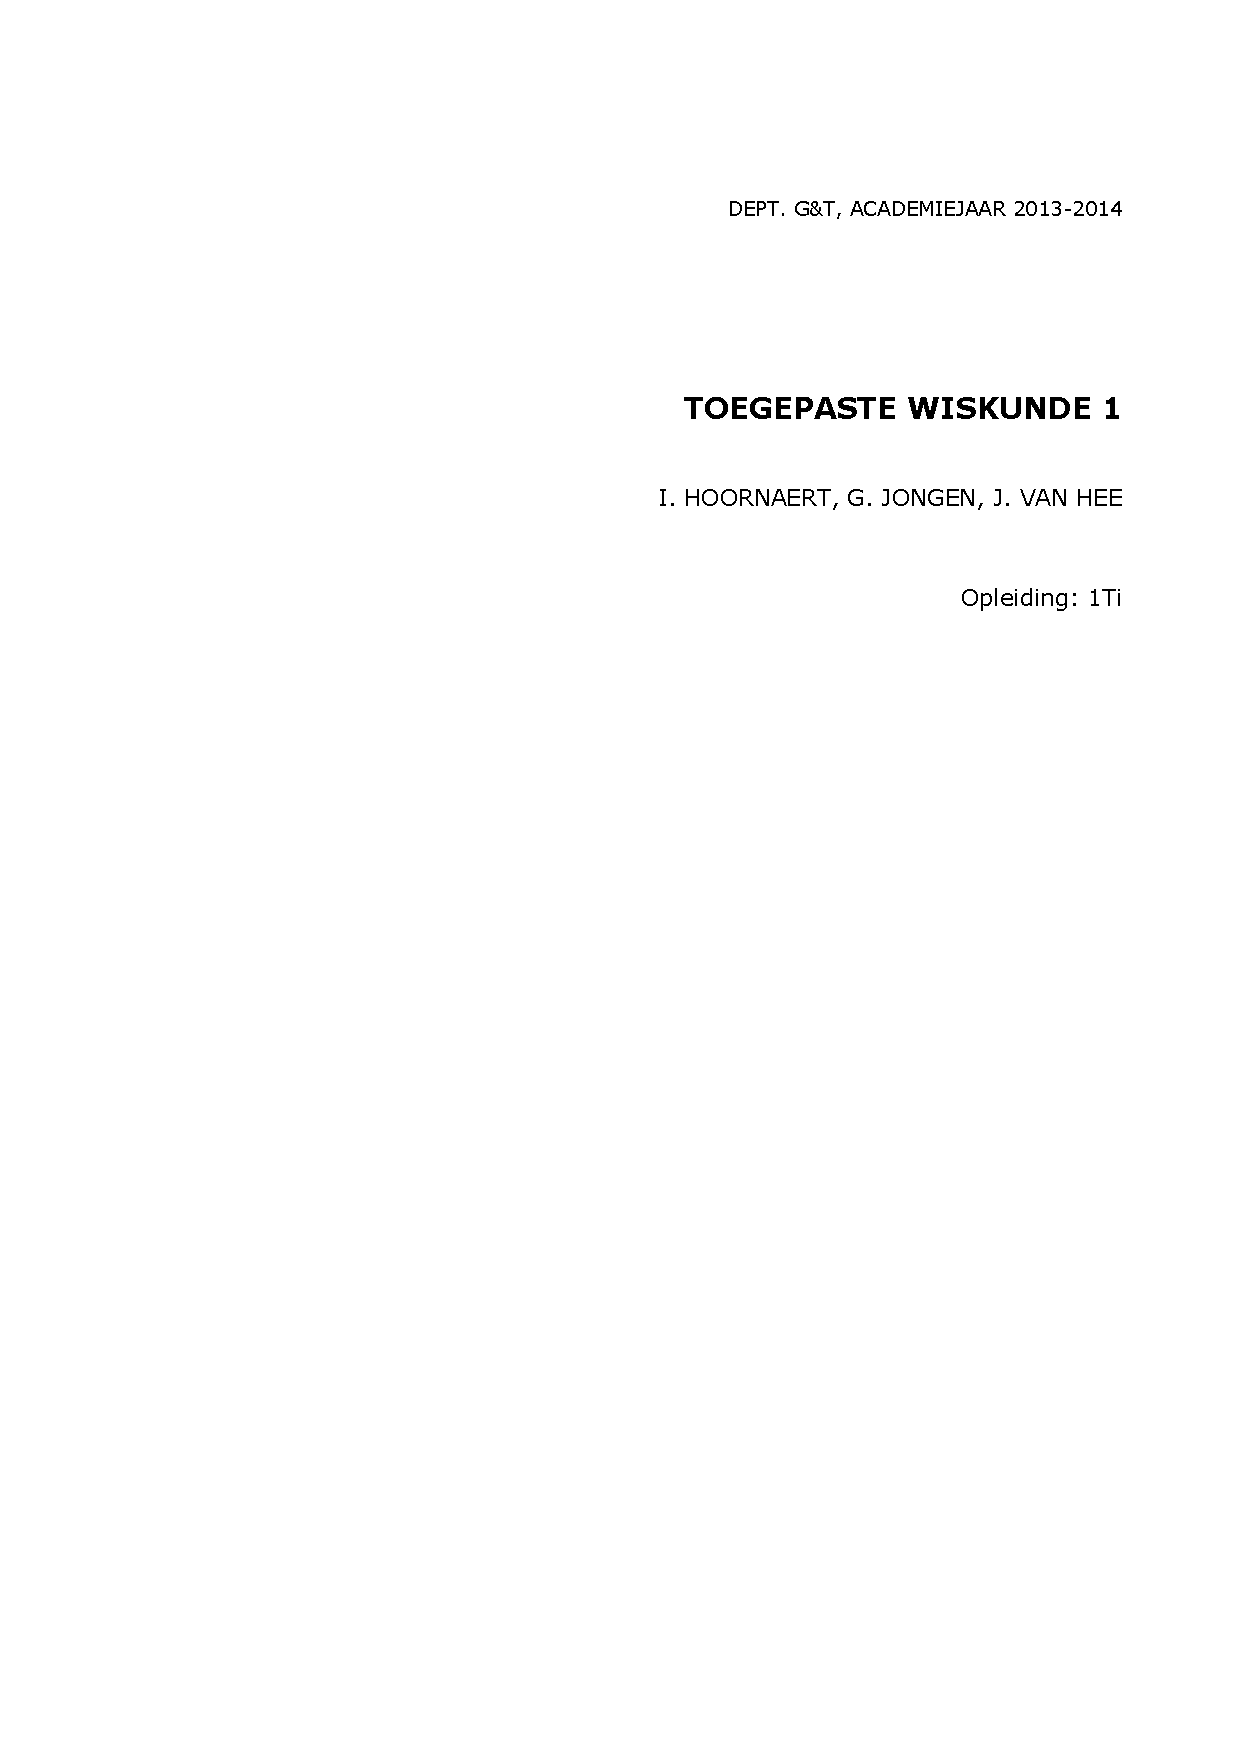
\includepdf{voorblad1314}
%%%%%%%%%%%%%%%%%%%%%%%%%%%%%%%%
% 14/9/05 [Jan]: aanpassingen, nieuwe vaknaam, Wim Bertels bijgevoegd,
%  academiejaar vervangen door semester, examens vervangen door examen,...
%
% 19/09/2004 [Jan]: aanpassing aan nieuw curriculum en verbeteren fouten
%
% 18 sept 03 [Jan]: foutjes verbeterd
%
% 18 sept 2002 [Jan]: bestand ge�ntegreerd in cursus, hoofding 
%	verzorgd met boxedminipage. Commentaren van Greetje weggelaten.
%
% aanpassingen van Greetje op 4/9/02 en 11/9
%
% Eerste blz. cursus wiskunde 1ti
% aangemaakt door Roos in september 2002
%%%%%%%%%%%%%%%%%%%%%%%%%%%%%%%

    \noindent
\setlength{\fboxsep}{.2cm} \noindent
\begin{boxedminipage}{\textwidth}
\begin{center}{\Large{\bf Informatieblad}}\end{center}
\textbf{Opleiding:} 1 Toegepaste informatica \\ \\
\textbf{Onderdeel:} Wiskunde - deel I \\ \\
\textbf{Titularissen:} W.~Bertels, J.~Van~Hee en R.~Wyseur
\end{boxedminipage}


\vspace{0.7cm} \noindent
    Wat de inhoud is van deze cursus vind je in de inhoudstafel maar
    we geven graag wat \textbf{accenten} mee zodat je weet waar je
    v\'{o}\'{o}r  staat.\\

    \noindent
    In dit vak beklemtonen we
    \begin{itemize}
    \item \textbf{logisch redeneren en zelfcontrole} en niet zozeer rekenvaardigheden.
    De zelfcontrole moet effici\"{e}nt gebeuren, o.a.\ via gebruik van wiskundige
    software;

    \item \textbf{oefeningen}. Ze helpen je begrippen
    en algoritmen aangebracht in de theorie op een grondige manier
    te verwerken. Bovendien leer je problemen geformuleerd in woorden
    om te zetten naar wiskundige vergelijkingen;

    \item  zowel het \textbf{analytisch} berekenen (via exacte
    methoden) als  het \textbf{benaderend} rekenen (numerieke iteratieve methoden,
    programmeerbaar) als het \textbf{grafisch} illustreren
    (grafieken). Deze verschillende werkwijzen om een
    probleem aan te pakken vullen elkaar goed aan.

    \end{itemize}

    \noindent
    We verwachten van je dat je \textbf{actief} aan de lessen \textbf{meewerkt}:
    \begin{itemize}
      \item je \textbf{analyseert}, \textbf{concretiseert}
      en/of \textbf{illustreert} de gedoceerde wiskundige begrippen door
      oefeningen op te lossen tijdens de les in kleine groepjes;
        \item je verwerkt \textbf{zelfstandig nieuwe leerstof}
        via werkteksten met doelgerichte opdrachten;
        \item je probeert thuis \textbf{nieuwe oefeningen}
        op te lossen.
    \end{itemize}
    \begin{quote}
    Feedback wordt op eenvoudige vraag gegeven. In de begeleidingsuren is er plaats voor een persoonlijke aanpak. Je kan hier individueel of samen met medestudenten vragen stellen, een moeilijke oefening bekijken, hulp vragen bij een minder eenvoudig stukje leerstof. Samen zoeken we hier naar die vorm van begeleiding waar je het meeste baat bij hebt. Soms betekent dit dat de docent je aanmoedigt en desnOPOs verplicht tot een gesprek. Durf in elk geval naar je docent stappen als je met vragen of opmerkingen zit. We zijn er om jou te helpen!
    \end{quote}


   \noindent Je behaalt je eindscore voor dit vak op volgende manier:
    \begin{enumerate}
    \item 30~\% van de punten staan op permanente evaluatie (PE). Deze
    punten verdien je \textbf{tijdens} het semester. Meer
    informatie vind je in het ``Informatieblad Permanente
    Evaluatie'';
    \item  de overige 70~\% van de punten verdien je tijdens het eindexamens in januari.
    Alleen de leerstof die niet in de werkteksten aan bod gekomen
    is, wordt hier ondervraagd.
    \end{enumerate}
\newpage

    \noindent
\setlength{\fboxsep}{.2cm} \noindent
\begin{boxedminipage}{\textwidth}
\begin{center}{\Large{\bf Permanente Evaluatie}}\end{center}
\textbf{Opleiding:} 1 Toegepaste informatica \\ \\
\textbf{Onderdeel:} Wiskunde - deel I\\ \\
\textbf{Titularissen:} W.~Bertels, J.~Van~Hee en R.~Wyseur
\end{boxedminipage}

\vspace{0.7cm} \noindent Quoteringen voor permanente evaluatie
worden toegekend op:
    \begin{itemize}
      
        \item  het persoonlijk verwerken via een begeleidende werktekst
        van een wiskundig onderwerp;

        \item enkele kleine opdrachten die in de loop van het
        semester worden opgegeven;

        \item de manier waarop je omspringt met feedback die
        gegeven wordt bij tussenresultaten van grote opdrachten 
        of eindresultaten van kleine opdrachten;

        \item werkzaamheid in de klas.

      \end{itemize}

\noindent Volgende afspraken gelden hierbij:
\begin{itemize}
\item de opdrachten worden \textbf{tijdens de lessen} gegeven.
Je bent zelf verantwoordelijk of je al dan niet tijdig op de
hoogte bent van een gegeven opdracht. Enkel in geval van overmacht
(bijv.\ ziekte) kunnen we uitzonderingen voorzien;

\item je geeft de opdracht steeds \textbf{persoonlijk} aan je docent af
(dus niet via de correspondentiebakjes);

\item als er een verslagje verwacht wordt, dan voldoet dit vanzelfsprekend aan de afgesproken regels die daaromtrent in de opleiding gelden (voorblad, duidelijke vermelding persoonlijke gegevens, goed taalgebruik,...);

\item je levert je werkje af \textbf{op het afgesproken tijdstip} (dag en uur).
\end{itemize}






\frontmatter
\tableofcontents
%%%%%%%%%%%%%%%%%%%%%%%%%%%%%%
%
% 5 sept 2013 [Jan] SAP-code, nieuwe collega, academiejaar aangepast
%
%%%%%%%%%%%%%%%%%%%%%%%%%%%%%%%

\chapter*{Studiewijzer}


\section*{Cursusfiche}
\begin{description}
\item[Academiejaar]2013--2014
\item[Opleiding]Bachelor in de Toegepaste informatica
\item[Opleidingsonderdeel]Toegepaste wiskunde 1 -- MBI71A
\item[Studiepunten]3
\item[Contacturen]26  (1 uur les in gewoon klaslokaal en 1 uur les in PC-klas per week gedurende 13 lesweken)	
\item[Semester]	1 
\item[SBU per studiepunt]	25
\item[Lectoren]I. Hoornaert, G. Jongen en J. Van Hee
\item[Beoogde competenties]$\qquad$

\begin{itemize}
\item De student verwerft wiskundige basisvaardigheden die nodig zijn bij andere opleidingsonderdelen.
\item De student kan gestructureerd een probleem aanpakken en het volledig en met zorg afwerken
\item De student kan zelf wiskundige eigenschappen ontdekken via gebruik van grafieken, berekeningen en gebruik van wiskundige software. Hij kan die eigenschappen ook correct toepassen in concrete situaties.
\item De student kan een algoritme zinvol toepassen en de beperkingen ervan in concrete situaties onderzoeken en bespreken.
\item De student kan adequaat vragen stellen, inspelen op antwoorden en kan bondig en overzichtelijk (schematisch) conclusies formuleren.
\item De student kan positief inspelen op gegronde feedback om zo het eigen leerproces bij te sturen. 
\end{itemize}

\item [Leerinhoud]$\qquad$

\begin{itemize}
\item \emph{Inleiding tot de verzamelingenleer}: definitie, `element zijn van', bewerkingen
\item \emph{Relaties}: definitie, soorten relaties, inverse relatie
\item \emph{Eerstegraadsfuncties}: wiskundig model, grafiek, functievoorschrift, snijpunt van twee rechten
\item \emph{Lineaire Programmering}: maximum-minimum problemen met beperkingen
\item \emph{Exponenti\"{e}le groei}: verband met lineaire groei, groeifactor en procentuele groei
\item \emph{Exponenti\"{e}le en logaritmische functies}: verloop van de functies en oplossen van eenvoudige exponenti\"{e}le en logaritmische vergelijkingen
\item \emph{Propositielogica}: proposities, waarheidswaarde, waarheidstabellen;
\item \emph{Meetkunde}: software P.e.L., eigenschappen van meetkundige figuren zoals veelhoeken en  cirkels, macro's maken en meetkundige plaatsen zoeken
\item \emph{Extremumproblemen}:  dynamische en grafische oplossing in PeL (zonder afgeleiden) 
\item \emph{Grafieken tekenen}: software Scilab
\end{itemize}

\item [Werkvormen]$\qquad$

\begin{itemize}
\item \emph{Overdracht}: activerend hoorcollege
\item \emph{Inoefenend}: student verwerkt leerstof met begeleide oefeningen

\end{itemize}



\item [Studiemateriaal]	$\qquad$

\begin{itemize}
\item Cursus `Toegepaste wiskunde 1': I. Hoornaert, G.~Jongen en J. Van Hee,  KHLeuven departement Gezondheidszorg \& Technologie, 2013
\item Website Meetkunde: http://wiskunde.khleuven.be 
\item Elektronisch leerplatform Toledo 
\end{itemize}

\item [Evaluatie]	In de studiegids vind je de aanduidingen van examentijdstippen, vorm van het examen, aandeel van de examenonderdelen (zoals permanente evaluatie, opdrachten en contactexamen).   Meer info vind je in de cursusbeschrijving die volgt.

\end{description}

\newpage
\section*{Cursusbeschrijving}
\subsection*{Situering van het opleidingsonderdeel}

Het opleidingsonderdeel `Toegepaste wiskunde 1' ondersteunt andere opleidingsonderdelen. Op een systematische manier worden begrippen, technieken en procedures ge\"{i}ntro\-du\-ceerd \emph{in een eenvoudige wiskundige omgeving}. Diezelfde competenties duiken later elders in het curriculum op in een meer complexe omgeving.
 
Er worden wiskundige begrippen en rekenvaardigheden opgefrist en aangeleerd die essentieel zijn voor iedere informaticus in spe. Verder komen eenvoudige problemen aan bod. De oplossingsmethoden daarvan bestaan uit opeenvolgende  stappen: 
\begin{enumerate}
\item wat is het probleem?
\item welke elementen zijn gekend om het probleem op te lossen?
\item hoe zet je dat om naar wiskundige uitdrukkingen?
\item welke stappen moeten gezet worden om tot de oplossing te komen?
\end{enumerate}

Op die manier wordt \emph{het logisch denken en de zelfcontrole} aangescherpt. Vraagstukken spelen tenslotte een belangrijke rol gezien de analogie met de analyse van een informaticaprobleem. 


\subsection*{Studiepunten}

Aan het opleidingsonderdeel (OPO) `Toegepaste wiskunde 1' zijn 3 studiepunten toegekend. Dit betekent dat je $3 \cdot 25=75$ uren moet werken voor dit OPO. Na aftrek van examen en lestijden komt dit neer op ongeveer 2,5 uur studietijd thuis per week.

\subsection*{Organisatie van de lessen}

Je hebt 2 keer 1 uur les theorie en oefeningen per week, afwisselend in een gewoon lokaal of PC-klas. Dit betekent dat verschillende hoofdstukken aan bod komen in de loop van \'{e}\'{e}n week. 

De docent geeft een kort overzicht over de begrippen of de oplossingsmethode die in die les aan bod komt. Daarna ga je zelf aan de slag. Er wordt veel aandacht besteed aan de \emph{logische structuur} van je oplossing. Je moet het ook mondeling kunnen toelichten. 

In de PC-klassen leer je werken met de software. Nadien gebruik je die om begeleid maar toch \emph{zelfstandig} meetkundige problemen op te lossen en oefeningen te illustreren.

\subsection*{Evaluatie}

De 20 punten voor dit opleidingsonderdeel worden volledig toegekend tijdens het  \emph{contactexamen} in januari. 
Het contactexamen is mondeling/schriftelijk met schriftelijke voorbereiding en legt de nadruk op probleemoplossend vermogen. Je mag gebruik maken van het formularium  en de softwarepakketten P.e.L.\ en Scilab.  Een kritische bespreking van je resultaat is belangrijk.
 
De docent geeft vooraf voldoende informatie over de vorm, de eisen qua structuur en volledigheid en de inhoud van het contactexamen.

\subsubsection*{Tweede examenkans (augustus)}
Je kan een tweede examenkans benutten om toch een credit te halen voor dit opleidingsonderdeel, of om je resultaat van januari te verbeteren.


%\include{formularium} is apart document...
%\tableofcontents

\mainmatter
\documentclass[dutch]{../khlslides}
\usepackage{graphicx}
\usepackage{pxfonts}
\usepackage{tikz}
\usepackage{calc}
\usepackage{fourier}

\usetikzlibrary{calc,shadows}


\title{Verzamelingenleer}
\author{Fr\'ed\'eric Vogels}
\logo{
\includegraphics[height=0.5cm]{../KHL.jpg}}
% \date{13 December 2012}
\institute[KHL]{KHLeuven}


\newcommand{\element}[3][]{
  \draw[fill=black] (#2) circle (.05);
  \node[anchor=south west,#1] at (#2) {#3};
}

\newcommand{\union}{\cup}
\newcommand{\intersect}{\cap}

\newcommand{\leftellipse}{(-2,0) ellipse (3cm and 2cm)}
\newcommand{\rightellipse}{(2,0) ellipse (3cm and 2cm)}

\pgfkeys{
  /tikz/.cd,
  highlight/.style={thick,fill=gray!50},
  outline/.style={thick,fill=none},
  empty/.style={thick,fill=white}
}

\begin{document}

\maketitle

{
\def\@#1{\mathrm{#1}}
\begin{frame}
  \frametitle{Basisoperatie}
  \begin{center}
    \begin{tikzpicture}[scale=.8,transform shape]
      \path[use as bounding box] (-4,-3) rectangle (4,3);
      \draw[ultra thick] (0,0) ellipse (4cm and 3cm);
      \node[anchor=south west] at (3,2) {\Huge A};
      \element{1,0}{a};
      \element{-2,1}{b};
      \element{2,-1}{c};
      \element{-1,0}{i};
      \element{0,2}{e};
      \element{0.5,-1}{h};
      \element{-1.5,-1.5}{g};

      \element{-4,-3}{f};
      \element{-3.5,3}{d};
      \element{4.5,-1}{j};
    \end{tikzpicture}
    \vskip5mm
     \[
      \begin{array}{c@{\qquad}c@{\qquad}c@{\qquad}c@{\qquad}c}
        \@a \in \@A & \@b \in \@A & \@c \in \@A & \@d \notin \@A & \@e \in \@A \\
        \@f \notin \@A & \@g \in \@A & \@h \in \@A & \@i \in \@A & \@j \notin \@A
      \end{array}
    \]
 \end{center}
\end{frame}
}

\begin{frame}
  \frametitle{Notaties}
  \begin{center}
    \begin{tikzpicture}[scale=.5,transform shape]
      \path[use as bounding box] (-4,-3) rectangle (4,3);
      \draw[ultra thick] (0,0) ellipse (4cm and 3cm);
      \node[anchor=south west] at (3,2) {\Huge A};
      \element{2,0.5}{2};
      \element{-2.5,1}{3};
      \element{1,-1}{5};
      \element{-1,0}{7};
      \element{0.5,1.5}{11};
      \element{0.5,-2}{13};
      \element{-1,-1.5}{17};

      \element{-4,-2.5}{0};
      \element{-3.25,3}{1};
      \element{4.5,-1}{4};
      \element{4.25,-1.75}{6};
      \element{.2,3.2}{8};
      \element{1,3.1}{9};
      \element{2,3.1}{10};
      \element{1,-3.5}{12};
      \element{.25,-3.6}{14};
      \element{-.5,-3.6}{15};
      \element{-2.75,-3}{16};
      \element{-2.5,3}{18};
    \end{tikzpicture}
  \end{center}
  \structure{Opsomming}
  \[ A = \left\{\; 2,3,5,7,11,13,17 \;\right\} \]
  \structure{Omschrijving}
  \[ A = \left\{\; x \;|\; x \leq 18 \textrm{ en } x \text{ is een priemgetal} \;\right\} \]
  \structure{Lege verzameling}
  \[ \emptyset = \{ \; \} \]
\end{frame}

\begin{frame}
  \frametitle{Gelijkheid}
  \begin{itemize}
    \item Twee verzamelingen $X$ en $Y$ zijn gelijk indien
          \[ \forall \; x. \; x \in X \iff x \in Y \]
          \vskip5mm
    \item In woorden
          \begin{center}
            $X$ en $Y$ zijn gelijk indien ze dezelfde elementen bevatten
          \end{center}
          \vskip5mm
    \item Notatie: $X = Y$
  \end{itemize}
\end{frame}

\begin{frame}
  \frametitle{Gevolgen}
  \begin{itemize}
    \item Een verzameling telt \emph{niet} hoe vaak een element voorkomt.
          \[ \{ 1, 1, 1, 1, 1 \} = \{ 1 \} \]
    \item Een verzameling definieert geen volgorde.
          \[ \{ 1, 2, 3 \} = \{ 3, 2, 1 \} \]
  \end{itemize}
\end{frame}

\begin{frame}
  \frametitle{Deelverzameling}
  \begin{center}
    \begin{tikzpicture}[scale=.6,transform shape]
      \draw[ultra thick] (0,0) ellipse (4cm and 3cm);
      % \node[anchor=south west] at (3,2) {\Huge A};

      \draw[ultra thick] (-1,0) ellipse (2cm and 1.5cm);
      % \node[anchor=south west] at (.5,1) {\Huge B};
    \end{tikzpicture}
  \end{center}
  \begin{itemize}
    \item $X$ is een deelverzameling van $Y$ indien elk element van $X$ ook voorkomt in $Y$
          \[
            \forall \; x. \; x \in X \rightarrow x \in Y
          \]
    \item Notatie: $X \subset Y$
  \end{itemize}
\end{frame}

\begin{frame}
  \frametitle{Gevolgen}
  \begin{itemize}
    \item De lege verzameling is deelverzameling van elke verzameling
          \[ \emptyset \subset X \]
          \vskip4mm
    \item Link met gelijkheid
          \[ X \subset Y \quad\textrm{en}\quad Y \subset X \qquad\iff\qquad X = Y \]
  \end{itemize}
\end{frame}

\begin{frame}
  \frametitle{Unie}
  \begin{center}
    \begin{tikzpicture}
      \draw[highlight] \leftellipse;
      \draw[highlight] \rightellipse;
      \draw[outline] (-2,0) \leftellipse;
    \end{tikzpicture}
  \end{center}
  \[
    X \union Y = \{ \; x \;|\; x \in X \;\mathrm{of}\; x \in Y \; \}
  \]
\end{frame}

\begin{frame}
  \frametitle{Doorsnede}
  \begin{center}
    \begin{tikzpicture}
      \begin{scope}
        \clip \leftellipse;
        \clip \rightellipse;
        \draw[highlight] \leftellipse;
        \draw[highlight] \rightellipse;
      \end{scope}
      \draw[outline] \leftellipse;
      \draw[outline] \rightellipse;
    \end{tikzpicture}
  \end{center}
  \[
    X \intersect Y = \{ \; x \;|\; x \in X \;\mathrm{en}\; x \in Y \; \}
  \]
  \begin{itemize}
    \item $X$ is \emph{conjunct} met $Y$ als $X \intersect Y \neq \emptyset$
    \item $X$ is \emph{disjunct} met $Y$ als $X \intersect Y = \emptyset$
  \end{itemize}
\end{frame}

\begin{frame}
  \frametitle{Verschil}
  \begin{center}
    \begin{tikzpicture}
      \draw[highlight] \leftellipse;
      \draw[empty] \rightellipse;
      \draw[outline] \leftellipse;
    \end{tikzpicture}
  \end{center}
  \[
    X - Y = \{ \; x \;|\; x \in X \;\mathrm{en}\; x \notin Y \; \}
  \]
\end{frame}

\begin{frame}
  \frametitle{Complement}
  \begin{center}
    \begin{tikzpicture}
      \draw[highlight] (-4,-3) rectangle (4,3);
      \draw[empty] (0,0) ellipse (3cm and 2cm);
    \end{tikzpicture}
  \end{center}
  \[
    X^c = \{ \; x \;|\; x \in U \;\mathrm{en}\; x \notin X \; \} = U - X
  \]
\end{frame}

\begin{frame}
  \frametitle{Cartesisch product}
  \begin{center}
    \begin{tikzpicture}
      \draw[outline] (-2,0) ellipse (1.5cm and 2cm);
      \node[anchor=south east] at (-2.5,1.8) {A};
      \draw[outline] (2,0) ellipse (1.5cm and 2cm);
      \node[anchor=south west] at (2.5,1.8) {B};

      \element[anchor=south east]{-2,0.5}{a}
      \element[anchor=south east]{-2,-0.5}{b}
      \element{2,1}{1}
      \element{2,0}{2}
      \element{2,-1}{3}

      \foreach \x in {0.5,-0.5} {
        \foreach \y in {1,0,-1} {
          \draw (-2,\x) -- (2,\y);
        }
      }
    \end{tikzpicture}
  \end{center}
  \[
    \begin{array}{rcl}
      \mathrm{A} & = & \left\{ \mathrm{a}, \mathrm{b} \right\} \\
      \mathrm{B} & = & \left\{ 1, 2, 3 \right\} \\
      \mathrm{A} \times \mathrm{B} & = & \left\{ ( \mathrm{a}, 1 ), (\mathrm{a}, 2 ), (\mathrm{a}, 3 ), ( \mathrm{b}, 1 ), (\mathrm{b}, 2 ), (\mathrm{b}, 3 ) \right\}
    \end{array}
  \]
  \vskip2mm
  \[
    X \times Y = \{ \; (x, y) \;|\; x \in X \;\mathrm{en}\; y \in Y \}
  \]
\end{frame}

\begin{frame}
  \frametitle{Rekenregels}
  \structure{Associativiteit}
  \[
    \begin{array}{rclclr}
      X \union (Y \union Z) & = & (X \union Y) \union Z & = & X \union Y \union Z \\
      X \intersect (Y \intersect Z) & = & (X \intersect Y) \intersect Z & = & X \intersect Y \intersect Z \\
    \end{array}
  \]
  \structure{Commutativiteit}
  \[
    \begin{array}{rcl}
      X \union Y & = & Y \union X \\
      X \intersect Y & = & Y \intersect X
    \end{array}
  \]
  \structure{Distributiviteit}
  \[
    \begin{array}{rcl}
      X \union (Y \intersect Z) & = & (X \union Y) \intersect (X \union Z) \\
      X \intersect (Y \union Z) & = & (X \intersect Y) \union (X \intersect Z) \\
    \end{array}
  \]
\end{frame}

\begin{frame}
  \frametitle{Rekenregels}
  \structure{Lege verzameling}
  \[
    \begin{array}{rclclr}
      X \union \emptyset & = & X \\
      X \intersect \emptyset & = & \emptyset \\
      X - \emptyset & = & X \\
      \emptyset - X & = & \emptyset \\
    \end{array}
  \]

  \structure{Wetten van de Morgan}
  \[
    \begin{array}{rclclr}
      (X \union Y)^c & = & X^c \intersect Y^c \\
      (X \intersect Y)^c & = & X^c \union Y^c \\
    \end{array}
  \]
\end{frame}

\begin{frame}
  \frametitle{Oefeningen}
  \begin{itemize}
    \item 1.2
    \item 1.4
    \item 1.6
    \item 1.9
    \item 1.10
    \item 1.12
    \item Rest: thuis
  \end{itemize}
\end{frame}

\end{document}



%%% Local Variables: 
%%% mode: latex
%%% TeX-master: t
%%% End: 

%%%%%%%%%%%%%%%%
% 5 sept 2013 [Jan] opmerkingen Greetje in theorie aangepast, stukje surjectie enz. toegev.
% 5 sept 2013 [Greetje] Oefeningen wat bijgewerkt
% sept 2013 [Jan]: OOD door OPO vervangen.
%
% 28/06/13 [Greetje] Oefeningen toegevoegd
% to do: injectie, bijectie surject herwerken
%%%%%%%%%%%%%%%%
 
 
\chapter{Relaties}
\label{chap:relatie}
\begin{quote}
\textit{Ha, nu gaat het leuk worden! dacht Alice. Ik ben blij dat ze raadsels gaan opgeven -- `Ik geloof dat ik het weet,' voegde ze er hardop aan toe.}

\textit{`Bedoel je dat je denkt dat je wel achter het antwoord kunt komen?' zei de Maartse Haas.}

\textit{`Precies, ja,' zei Alice.}

\textit{`Zeg dan meteen wat je bedoelt,' ging de Maartse Haas voort.}

\textit{`Dat doe ik toch,' gaf Alice haastig ten antwoord, `tenminste -- tenminste, ik bedoel wat ik zeg -- dat komt op hetzelfde neer, hoor.'}

\textit{`Helemaal niet hetzelfde! zei de Hoedenmaker. `Dan zou je met evenveel recht kunnen zeggen dat ``Ik zie wat ik eet'' op hetzelfde neerkomt als ``Ik eet wat ik zie''!'}

          Uit `Alice in Wonderland' -- Lewis Carroll
\end{quote}



\newpage
 \section{Definitie}
 \label{sec:defRelatie}
Het voorbeeld van de verzameling van postcodes en bijhorend inwonersaantal (sectie~\ref{sec:prodverz} op pagina~\pageref{pg:postcodes}), is een deelverzameling van de productverzameling  $\nat\times\nat$. Zo'n deelverzameling van een productverzameling noemen we een \emph{relatie}\index{relatie}.

Voorbeelden:
\begin{itemize}
  \item $A=\{1,2,3\}$ en $B=\{\text{a}, \text{b}\}$. De verzameling $\{(1, \text{a}), (2,\text{a}),(2,\text{b}),(3,\text{b)}\}$
        is een relatie van de verzameling $A$ naar\footnote{In plaats van het woord `naar' mag je ook `op' gebruiken en dus spreken over `de relatie van de verzameling $A$ op de verzameling $B$'.} de verzameling $B$.
  \item $A=\{0,1\}$, $B=\{\mathrm{a},\mathrm{b}\}$, $C=\{7,8,9\}$. De verzameling
        \[ \{(0,\mathrm{a},8), (0,\mathrm{a},9), (1,\mathrm{b},8) \} \]
        is een relatie op de verzamelingen $A$, $B$ en $C$.
  \item $A=\nat_0$, $B$ de verzameling van strings met lengte 20 (spatie toegelaten),
       $C=\{10,11,12,\dots,90\}$. Dan kan je met een relatie op de verzamelingen $A, B, C$ en $B$ de leden van de zwemclub omschrijven (inschrijvingsnummer, naam, leeftijd, woonplaats).
\end{itemize}

Het concept van relatie is de basis van de relationele databank, onderwerp van het OPO `Technieken van datamodellering'. De gegevens van \'e\'en rij worden gezien als een geordend $n$-tal. Alle rijen samen vormen een deelverzameling van de productverzameling van de  datatypes van de verschillende kolommen.

Als een relatie paren bevat, spreken we van een \emph{binaire relatie}\index{relatie!binair}\index{binaire relatie}, bijvoorbeeld
\begin{itemize}
\item $A=\{\mathrm{Jan},\mathrm{Pol},\mathrm{Anne}\}$ en $B=\nat$. De verzameling
      \[ \{(\mathrm{Jan},10),(\mathrm{Pol},6),(\mathrm{Anne},11) \} \]
      is een binaire relatie. Deze relatie is een deelverzameling van de productverzameling $A\times B$.
\end{itemize}
We spreken in zo'n geval ook over een relatie van $A$ \emph{naar} $B$. De elementen van $A$ worden \emph{afgebeeld} op de elementen van $B$.
De verzameling $A$ is de \emph{bronverzameling}\index{bronverzameling}\index{relatie!bronverzameling},
de verzameling $B$ de \emph{doelverzameling}\index{doelverzameling}\index{relatie!doelverzameling}. Als $(a,b)$ element is van de relatie, zeggen we dat $b$ het \emph{beeld}\index{beeld} is van $a$.

De idee van `een relatie van $A$ naar $B$' en `het punt $a$ wordt afgebeeld op $b$' breiden we uit naar relaties op meer dan twee verzamelingen. 

\begin{samepage}
Voorbeelden:
\begin{itemize}
  \item De relatie $U=\{(1,2,3),(2,3,5),(4,5,9), (5,6,11),\dots\}$ is een deelverzameling
        van de productverzameling $\nat\times\nat\times\nat$.
        Het derde getal van het drietal $(a,b,c)$ is gelijk aan de som van de twee
        voorgaande getallen: $c=a+b$. De getallen $a$ en $b$ worden afgebeeld op $c$.
  \item De verzameling $V$ met elementen
        \[ \{(\text{rood},\text{blauw},\text{magenta}), (\text{rood},\text{groen},\text{geel}), (\text{groen},\text{blauw},\text{cyaan}),\dots\} \]
        is een deelverzameling van $A\times A\times B$ waarbij $A$ de verzameling van primaire kleuren is en $B$ de verzameling van secundaire kleuren:
        twee primaire kleuren vormen een secundaire kleur. De relatie $V$ beeldt twee primaire kleuren af op een secundaire kleur.
\end{itemize}
\end{samepage}

We geven ten slotte nog enkele voorbeelden van relaties, gegrepen uit het dagelijkse leven:
\begin{itemize}
\item de relatie die de snelheid van een auto afbeeldt op zijn verbruik;
\item de relatie die de mazoutprijs weergeeft in functie van de tijd;
\item de relatie die de kostprijs van een online bestelling van foto's (verzendingskosten inbegrepen) toont naargelang het aantal bestelde foto's.
\end{itemize}

\section{Domein en bereik}
\label{sec:domeinBereik}
Gegeven de binaire relatie $U=\{({a},{b})|{a}\in A \mathrm{~ en~} {b} \in B\}\subset A \times B$. 
Het \emph{domein}\index{domein}\index{relatie!domein} van de relatie $U$ is de verzameling van de elementen~${a}$ waarvoor er een $b\in B$ 
bestaat zodat het paar $({a},{b})\in U$. We noteren het domein van $U$ met $\dom{U}$.

Het \emph{bereik}\index{bereik}\index{relatie!bereik} van de relatie $U$ is de verzameling van de elementen~${b}$
waarvoor er een $a\in A$ bestaat zodat het paar $({a},{b})\in U$. Het bereik wordt ook vaak het \emph{beeld}\index{beeld}\index{relatie!beeld} van $U$ genoemd.
Notatie: $\range{U}$ of $\text{Bld}(U)$.

Voorbeeld: voor de relatie $U=\{(1,\mathrm{a}),(1,\mathrm{b}),(2,\mathrm{b}),(4,\mathrm{b}) \}$ van $A=\{1,2,3,4\}$ op $B=\{\mathrm{a},\mathrm{b},\mathrm{c} \}$ is 
\begin{itemize}
\item het domein gelijk aan $\dom{U}=\{1,2,4\}$. Dit zijn de elementen van $\mathbf{A}$ waar een pijl \textbf{vertrekt} (figuur~\ref{fig:dombereik}).
\item het bereik gelijk aan $\range{U}=\{ \mathrm{a},\mathrm{b}\}$. Dit zijn de elementen van $\mathbf{B}$ waar een pijl \textbf{aankomt} (figuur~\ref{fig:dombereik}).
\end{itemize}

\begin{figure}[htbp]
\centering
% Figuur domein en bereik
\begin{tikzpicture}[thick]
\draw \vertellipl node [above=2.3cm, left] {$A$};
\draw \vertellipr node [above=2.3cm, left] {$B$};
% linkse elementen
\draw[fill] (0,1.3) \bol node [above] {1};
\draw[fill] (0,0.4) \bol node [above] {2};
\draw[fill] (0,-0.5) \bol node [above] {3};
\draw[fill] (0,-1.4) \bol node [above] {4};
% rechtse elementen
\draw[fill] (3,1) \bol node [above] {a};
\draw[fill] (3,0) \bol node [above] {b};
\draw[fill] (3,-1) \bol node [above] {c};
% pijlen
\begin{scope}[decoration={
    markings,
    mark=at position 0.5 with {\arrow{>}}}
    ] 
    \draw[postaction={decorate}] (0,1.3) to (3,1);
    \draw[postaction={decorate}] (0,1.3) to (3,0);
    \draw[postaction={decorate}] (0,0.4) to (3,0);
    \draw[postaction={decorate}] (0,-1.4) to (3,0);
\end{scope}
\end{tikzpicture}
\caption{Relatie: domein = \{1,2,4\} en bereik = \{a,b\}}
\label{fig:dombereik}
\end{figure}


\section{Soorten relaties} \label{subsec:soortenrelaties}\index{relatie!soorten}
In het voorgaande stelden we geen voorwaarden aan het aantal vertrekkende (in bronverzameling) en toekomende pijlen (in doelverzameling) en noemden we alles `relatie'. Je kan echter wel een aantal bijzondere relaties onderscheiden. 

Als we ons richten naar de \emph{bron}verzameling kunnen we een onderscheid maken tussen afbeeldingen en functies. Verleggen we de focus naar de \emph{doel}ver\-za\-me\-ling, dan kunnen we de begrippen injectief, surjectief en bijectief definiëren.

\subsection{Functie, afbeelding} \label{subsec:functies}
Gegeven twee verzamelingen $A$ en $B$ en een relatie van $A$ op $B$. We bekijken enkel de elementen uit de bronverzameling $A$. Je kan nu drie gevallen onderscheiden:
\begin{enumerate}
  \item Als elk element van $A$ \emph{hoogstens} één beeld heeft, noemen we de relatie een \textbf{functie}\index{functie}. In de pijlenvoorstelling vertrekt uit elk element van $A$ ten hoogste één pijl.
  \item Als elk element van $A$ \emph{juist} één beeld heeft, noemen we deze speciale relatie een \textbf{afbeelding}\index{afbeelding}.
        In de pijlenvoorstelling vertrekt uit elk element van $A$ juist één pijl. Elke afbeelding is dus een functie. Geldt het omgekeerde ook: is elke functie ook een afbeelding\footnote{Nee, natuurlijk! Leg zelf uit waarom.}?
  \item Een relatie die niet aan één van beide bovenstaande voorwaarden voldoet (er zijn elementen in $A$ die meerdere beelden hebben en dus vertrekken er uit die elementen meer dan één pijl) is een gewone relatie.
\end{enumerate}

\subsection{Surjectief, injectief, bijectief} \label{subsec:jectief}
Gegeven twee verzamelingen $A$ en $B$ en een relatie van $A$ op $B$. We bekijken dit keer enkel de elementen uit de doelverzameling $B$. Je kan nu volgende gevallen onderscheiden:
\begin{enumerate}
  \item Als elk element van de doelverzameling $B$ het beeld is van \emph{minstens} één element van $A$ noemen we de relatie \textbf{surjectief}\index{surjectie}\footnote{Een mogelijk trucje om dit te onthouden is de betekenis van het Franse woord `sur' (op). Elk element van $B$ krijgt minstens één pijl en dus is het bereik van de relatie de doelverzameling $B$ zelf. Het is alsof het bereik \emph{op} de doelverzameling valt en die helemaal bedekt.}. In de pijlenvoorstelling komt in elk element van $B$ minstens één pijl toe.
  \item Als elk element van $B$ het beeld is van \emph{hoogstens} één element van $A$ spreken we van een \textbf{injectieve}\index{injectie} relatie. In elk element van $B$ komt hoogstens één pijl toe. Het is dus mogelijk dat er elementen in $B$ zijn waar geen pijl toekomt.
  \item Combineer bovenstaande eisen en je krijgt een \textbf{bijectieve}\index{bijectie} relatie: elk element uit $B$ is het beeld van juist één element uit $A$. In elk element van $B$ komt juist één pijl toe. Een bijectieve relatie is zowel surjectief als injectief.
\end{enumerate}

\subsection{Surjectie, injectie, bijectie}
Uit het aantal vertrekkende pijlen van de elementen van de bronverzameling (sectie~\ref{subsec:functies}) kan je opmaken of de relatie een functie of afbeelding (of geen van beiden) is. In sectie~\ref{subsec:jectief} definieerden we de begrippen surjectief, injectief en bijectief die iets vertellen over het aantal aankomende pijlen in de elementen van de doelverzameling.

Als de relatie een afbeelding is, kom je tot volgende veel gebruikte termen:
\begin{description}
\item[surjectie:] een surjectieve afbeelding
\item[injectie:] een injectieve afbeelding
\item[bijectie:] een bijectieve afbeelding
\end{description}


\subsection{Voorbeelden}
\subsubsection*{Voorbeeld 1}
Gegeven de verzameling $B$ van alle wachtwoorden $y_i$ die in G\&T gebruikt worden om in te loggen op de pc's en $A$ de verzameling van alle ge\-brui\-kers\-accounts~$x_i$. Beschrijf de relatie ``Account \ldots \ heeft als wachtwoord \ldots ''.

Elke account heeft juist één wachtwoord en dus is deze relatie een afbeelding: uit elk element van $A$ (elke account) vertrekt juist één pijl.
Sommige mensen hebben misschien toevallig hetzelfde wachtwoord gekozen voor hun account maar elk wachtwoord wordt zeker één keer gebruikt. Het is dus mogelijk dat er meerdere pijlen toekomen in elementen van $B$. Dit voldoet aan de voorwaarde voor een surjectieve relatie.

We vatten samen: deze relatie is een surjectieve afbeelding, of kortweg `surjectie'. In databankenterminologie noemt men dit een `veel-op-één relatie'.
\begin{figure}[htbp]
\centering
    % Figuur veel-op-een relatie
\begin{tikzpicture}[thick]
\draw \grvertellipl node [above=3.3cm, left] {$A$};
\draw \grvertellipr node [above=3.3cm, left] {$B$};
% rechtse elementen
\draw[fill] (4,2) \bol node [above] {$y_1$};
\draw[fill] (4,0) \bol node [above] {$y_2$};
\draw[fill] (4,-2) \bol node [above] {$y_3$};
% linkse elementen
\draw[fill] (0,2.3) \bol node [above] {$x_1$};
\draw[fill] (0,1.4) \bol node [above] {$x_2$};
\draw[fill] (0,0.5) \bol node [above] {$x_3$};
\draw[fill] (0,-0.4) \bol node [above] {$x_4$};
\draw[fill] (0,-1.3) \bol node [above] {$x_5$};
\draw[fill] (0,-2.2) \bol node [above] {$x_6$};
% pijlen
\begin{scope}[decoration={
    markings,
    mark=at position 0.5 with {\arrow{>}}}
    ] 
    \draw[postaction={decorate}] (0,2.3) to (4,2);
    \draw[postaction={decorate}] (0,1.4) to (4,2);
    \draw[postaction={decorate}] (0,0.5) to (4,2);
    \draw[postaction={decorate}] (0,-0.4) to (4,0);
    \draw[postaction={decorate}] (0,-1.3) to (4,-2);
    \draw[postaction={decorate}] (0,-2.2) to (4,-2);
\end{scope}
\end{tikzpicture}
\caption{Een surjectieve afbeelding}
\label{fig:surjectie}
\end{figure}


\subsubsection*{Voorbeeld 2}
Als $A=\{\mathrm{rood},\mathrm{oranje},\mathrm{geel}\}$ en $B=\{\mathrm{a},\mathrm{g},\mathrm{r}\}$, wat is dan de relatie $U=\{({x},{y})\mid \mathrm{kleur~}x\mathrm{~bevat~de~letter~}y\}$?

Figuur \ref{fig:surjectieverel} toont een grafische weergave van deze relatie. Uit het element oranje vertrekken twee pijlen. De relatie is dus geen functie of afbeelding. Als je naar de doelverzameling kijkt, merk je dat er in elk element minstens één pijl toekomt. De relatie is dus \emph{surjectief}, maar omdat het geen afbeelding is mag je dit geen  `surjectie' noemen.
\begin{figure}[htbp]
\centering
    % Figuur geen veel-op-een relatie
\begin{tikzpicture}[thick]
\draw \grvertellipl node [above=3.3cm, left] {$A$};
\draw \grvertellipr node [above=3.3cm, left] {$B$};
% rechtse elementen
\draw[fill] (4,2) \bol node [above] {a};
\draw[fill] (4,0) \bol node [above] {g};
\draw[fill] (4,-2) \bol node [above] {r};
% linkse elementen
\draw[fill] (0,2) \bol node [above] {rood};
\draw[fill] (0,0) \bol node [above] {oranje};
\draw[fill] (0,-2) \bol node [above] {geel};
% pijlen
\begin{scope}[decoration={
    markings,
    mark=at position 0.5 with {\arrow{>}}}
    ] 
    \draw[postaction={decorate}] (0,2) to (4,-2);
    \draw[postaction={decorate}] (0,0) to (4,2);
    \draw[postaction={decorate}] (0,0) to (4,-2);
    \draw[postaction={decorate}] (0,-2) to (4,0);
\end{scope}
\end{tikzpicture}
\caption{Een surjectieve relatie}
\label{fig:surjectieverel}
\end{figure}


\subsubsection*{Voorbeeld 3}
Beschouw als bronverzameling de pasfoto's die genomen worden bij de inschrijvingen aan de KHLeuven. De doelverzameling is alle studentennummers. Welke relatie wordt voorgesteld door ``\ldots \ is de pasfoto die hoort bij student \ldots ''.

Bij elke pasfoto hoort juist één nummer en dus is deze relatie een afbeelding. Omgekeerd is elk studentennummer ook het beeld van één foto en dus is deze afbeelding ook bijectief. Een bijectieve afbeelding noemt men kortweg een `bijectie'. In databankentaal spreekt men over een `één-op-één relatie'.

\subsubsection*{Voorbeeld 4}
Wat voor een relatie is $U$?
\[
U=\left\{(x,y)\mid x,y\in\real \mathrm{~en~} y=x^2\right\}.
\]

Elke $x$ uit de bronverzameling ($\real$) heeft een beeld, dus dit is een afbeelding (functie). Aan de kant van de doelverzameling merk je dat er $y$-waarden zijn die geen beeld kunnen zijn van elementen $x$, zoals negatieve getallen: $-1$ kan nooit het kwadraat zijn van een reëel getal. Hieruit volgt dat deze afbeelding niet surjectief is. Anderzijds zijn er $y$-waarden die het beeld zijn van twee verschillende $x$-waarden: $4$ is zowel het beeld van $2$ als van $-2$. De afbeelding is dus ook niet injectief. We besluiten: de relatie $U$ is een afbeelding.

\subsubsection*{Voorbeeld 5}
We passen voorbeeld 4 lichtjes aan en bekijken de relatie $V$:
\[
V=\left\{(x,y)\mid x\in\real, y\in\real^+ \mathrm{~en~} y=x^2\right\}.
\]

Wat is het verschil tussen $U$ uit het vorig voorbeeld en deze relatie $V$? De doelverzameling wordt beperkt tot de positieve reële getallen ($\real^+$). Deze keuze heeft echter een effect op de relatie.

We kunnen de uitleg uit vorig voorbeeld hernemen om te besluiten dat $V$ een afbeelding is. Door de beperking van de doelverzameling tot $\real^+$ is elke $y$ nu het beeld van minstens één $x$. Deze afbeelding is dus surjectief (kortweg `surjectie').

\subsubsection*{Voorbeeld 6}
Laten we iets verder gaan in het aanpassen van de vorige relatie tot:
\[
W=\left\{(x,y)\mid x\in\real^+, y\in\real \mathrm{~en~} y=x^2\right\}.
\]

Elke $x$ heeft juist één beeld, dus deze relatie is een afbeelding. Wat de doelverzameling betreft: elke $y$ is het beeld van juist één $x$ ($4$ is het kwadraat van $2$) of is geen beeld ($-1$ kan nooit het kwadraat zijn van een positief reëel getal). Dit voldoet aan de definitie van injectiviteit. Bijgevolg is $W$ een injectieve afbeelding, of kortweg `injectie'.

Denk bij wijze van oefening eens na hoe je de bron- en of doelverzameling moet aanpassen om van deze relatie een bijectie te maken?








%\section{Soorten relaties}
%\label{subsec:soortenrelaties}
%
%Binnen relationele databanken en ERD, het bijhorende entity-relationship 
%diagram worden relaties  onderscheiden naargelang \'e\'en of meer 
%elementen uit de bronverzameling op \'e\'en of meer elementen uit de 
%beeldverzameling worden afgebeeld. In wat volgt wordt er enkel gesproken 
%over binaire relaties. De idee\"en kunnen uitgebreid worden naar andere 
%relaties.
%
%\subsection{Veel-op-veel relaties}
%Bij een veel-op-veel relatie (in de notatie van ERD: $N..  N$) 
%wordt elk element uit de bronverzameling  op \'e\'en of meerdere 
%elementen uit de beeldverzameling afgebeeld (figuur~\ref{fig:veelopveelvb}). Ieder element uit de beeldverzameling is één of meerdere keren beeld van een element uit de bronverzameling. Het kan zijn dat elementen uit de bronverzameling geen beeld hebben en dat elementen uit de beeldverzameling geen beeld zijn. 
%Enkele voorbeelden:
%\begin{itemize}
%\item de relatie `leverancier levert biermerk': iedere leverancier levert meerdere biermerken en ieder biermerk wordt door meerdere leveranciers geleverd
%\item de relatie `lector geeft les aan student van KHLeuven'
%\end{itemize}
%
%\begin{figure}[htbp]
%\centering
%    % Figuur veel-op-veel relatie
\begin{tikzpicture}[thick]
\draw \grvertellipl node [above=3.3cm, left] {$A$};
\draw \grvertellipr node [above=3.3cm, left] {$B$};
% linkse elementen
\draw[fill] (0,2) \bol node [above] {$x_1$};
\draw[fill] (0,0) \bol node [above] {$x_2$};
\draw[fill] (0,-2) \bol node [above] {$x_3$};
% rechtse elementen
\draw[fill] (4,2.3) \bol node [above] {$y_1$};
\draw[fill] (4,1.4) \bol node [above] {$y_2$};
\draw[fill] (4,0.5) \bol node [above] {$y_3$};
\draw[fill] (4,-0.4) \bol node [above] {$y_4$};
\draw[fill] (4,-1.3) \bol node [above] {$y_5$};
\draw[fill] (4,-2.2) \bol node [above] {$y_6$};
% pijlen
\begin{scope}[decoration={
    markings,
    mark=at position 0.5 with {\arrow{>}}}
    ] 
    \draw[postaction={decorate}] (0,2) to (4,2.3);
    \draw[postaction={decorate}] (0,2) to (4,1.4);
    \draw[postaction={decorate}] (0,2) to (4,0.5);
    \draw[postaction={decorate}] (0,0) to (4,-0.4);
    \draw[postaction={decorate}] (0,-2) to (4,-1.3);
    \draw[postaction={decorate}] (0,-2) to (4,-2.2);
    \draw[postaction={decorate}] (0,-0) to (4,1.4);
    \draw[postaction={decorate}] (0,-0) to (4,0.5);
    \draw[postaction={decorate}] (0,-2) to (4,1.4);
    \draw[postaction={decorate}] (0,0) to (4,-2.2);
\end{scope}
\end{tikzpicture}
%\caption{Veel-op-veel relatie}
%\label{fig:veelopveelvb}
%\end{figure}
%
%
%\subsection{E\'en-op-veel relaties}
%Bij een \'e\'en-op-veel relatie ($1..N$) heeft ieder element van de bronverzameling  \'e\'en of meerdere beelden (figuur~\ref{fig:eenopveel}). Een element van de beeldverzameling is maar beeld van \'e\'en element van de bronverzameling.
%
% Enkele voorbeelden:
%\begin{itemize}
%\item de relatie `leerling is eigenaar van e-mail adres'
%\item de relatie `vrouw is moeder van kind'
%\end{itemize}
%\begin{figure}[htbp]
%\centering
%% Figuur een-op-veel relatie
\begin{tikzpicture}[thick]
\draw \grvertellipl node [above=3.3cm, left] {$A$};
\draw \grvertellipr node [above=3.3cm, left] {$B$};
% linkse elementen
\draw[fill] (0,2) \bol node [above] {$x_1$};
\draw[fill] (0,0) \bol node [above] {$x_2$};
\draw[fill] (0,-2) \bol node [above] {$x_3$};
% rechtse elementen
\draw[fill] (4,2.3) \bol node [above] {$y_1$};
\draw[fill] (4,1.4) \bol node [above] {$y_2$};
\draw[fill] (4,0.5) \bol node [above] {$y_3$};
\draw[fill] (4,-0.4) \bol node [above] {$y_4$};
\draw[fill] (4,-1.3) \bol node [above] {$y_5$};
\draw[fill] (4,-2.2) \bol node [above] {$y_6$};
% pijlen
\begin{scope}[decoration={
    markings,
    mark=at position 0.5 with {\arrow{>}}}
    ] 
    \draw[postaction={decorate}] (0,2) to (4,2.3);
    \draw[postaction={decorate}] (0,2) to (4,1.4);
    \draw[postaction={decorate}] (0,2) to (4,0.5);
    \draw[postaction={decorate}] (0,0) to (4,-0.4);
    \draw[postaction={decorate}] (0,-2) to (4,-1.3);
    \draw[postaction={decorate}] (0,-2) to (4,-2.2);
\end{scope}
\end{tikzpicture}
%\caption{E\'en-op-veel relatie}
%\label{fig:eenopveel}
%\end{figure}
%
%Als niet ieder element van de bronverzameling een beeld heeft, spreken we van de \emph{optionele} \'e\'en-op-veel relatie ($0..N$). Zo kan een vrouw ook geen kinderen hebben.
%
%
%\subsection{Functies  en veel-op-\'e\'en relaties}
%\label{subsec:functies}
%In de hierboven beschreven relaties kan een element uit de bronverzameling meerdere beelden hebben in de beeldverzameling. Dat is niet altijd praktisch. 
%
%In een database worden bijvoorbeeld  gebruikersnamen (positief geheel getal)
% opgeslagen die geregistreerd zijn. 
%Als je  een relatie gebruikt om een gebruikersnaam uit de database te 
%verbinden aan een wachtwoord (string met lengte kleiner dan 20), 
%dan kan elke gebruikersnaam \emph{juist \'e\'en keer} gekoppeld worden 
%aan een wachtwoord (iedere gebruiker kan maar \'e\'en zinvol wachtwoord 
%hebben). Als de admin de gebruikers registreert, kan het voorkomen dat een gebruiker nog geen wachtwoord heeft. Eenzelfde wachtwoord  mag 
%evenwel aan verschillende gebruikersnamen verbonden worden. In de 
%relatie van `gebruikte gebruikersnamen' op `gebruikte wachtwoorden' 
%heeft ieder gebruikersnaam dus  \emph{hoogstens} \'e\'en beeld, maar 
%kan een `gebruikt wachtwoord' beeld zijn van meerdere `gebruikte 
%gebruikersnamen'. Dit soort relatie noemen we een 
%\emph{ veel-op-\'e\'en relatie}.
%
%\begin{quote}
%Bij een  veel-op-\'e\'en relatie ($N..1$) heeft ieder element uit de bronverzameling juist \'e\'en beeld en is ieder element uit de beeldverzamelingen beeld  van één of meerdere elementen uit de bronverzameling (figuur~\ref{fig:veelopeen2}).
%\end{quote}
%
%\begin{quote}
%Bij een  \emph{optionele} veel-op-\'e\'en relatie ($N..0$) heeft ieder element uit de bronverzameling \'e\'en  beeld, maar moet niet  elk element uit de beeldverzamelingen beeld zijn van één of meerdere elementen uit de bronverzameling.
%\end{quote}
%
%Merk op dat iedere veel-op-één relatie ook een \emph{optionele} veel-op-één relatie is.
%
%\begin{figure}[htbp]
%\centering
%    % Figuur veel-op-een relatie
\begin{tikzpicture}[thick]
\draw \grvertellipl node [above=3.3cm, left] {$A$};
\draw \grvertellipr node [above=3.3cm, left] {$B$};
% rechtse elementen
\draw[fill] (4,2) \bol node [above] {$y_1$};
\draw[fill] (4,0) \bol node [above] {$y_2$};
\draw[fill] (4,-2) \bol node [above] {$y_3$};
% linkse elementen
\draw[fill] (0,2.3) \bol node [above] {$x_1$};
\draw[fill] (0,1.4) \bol node [above] {$x_2$};
\draw[fill] (0,0.5) \bol node [above] {$x_3$};
\draw[fill] (0,-0.4) \bol node [above] {$x_4$};
\draw[fill] (0,-1.3) \bol node [above] {$x_5$};
\draw[fill] (0,-2.2) \bol node [above] {$x_6$};
% pijlen
\begin{scope}[decoration={
    markings,
    mark=at position 0.5 with {\arrow{>}}}
    ] 
    \draw[postaction={decorate}] (0,2.3) to (4,2);
    \draw[postaction={decorate}] (0,1.4) to (4,2);
    \draw[postaction={decorate}] (0,0.5) to (4,2);
    \draw[postaction={decorate}] (0,-0.4) to (4,0);
    \draw[postaction={decorate}] (0,-1.3) to (4,-2);
    \draw[postaction={decorate}] (0,-2.2) to (4,-2);
\end{scope}
\end{tikzpicture}
%\caption{Veel-op-\'e\'en relatie}
%\label{fig:veelopeen2}
%\end{figure}
%
%We geven enkele voorbeelden:
%\begin{itemize}
%\item Als $A=\{1,-1,2,-2,3,-3\}$ en $B=\{1,2,4,5,8,9\}$, dan is de relatie $U=\{({x},\mathrm{y})\mid {y}={x}^2\}$ een veel-op-\'e\'en relatie (figuur~\ref{fig:afbeelding1}).
%\item Als $A=\{\mathrm{rood},\mathrm{oranje},\mathrm{geel}\}$ en $B=\{\mathrm{a},\mathrm{g},\mathrm{r}\}$, dan is de relatie $U=\{({x},{y})\mid \mathrm{kleur~}x\mathrm{~bevat~de~letter~}y\}$ \emph{geen} veel-op-\'e\'en relatie (figuur~\ref{fig:afbeelding2}).
%\item de relatie die kinderen afbeeldt op hun moeder: ieder kind heeft 1 vrouw als moeder en een vrouw kan moeder zijn van verschillende kinderen
%\item de relatie `leerling zit in klas': elke leerling zit in 1 klas\footnote{waarbij we aannemen dat je geen aangepast jaarprogramma volgt en verschillende vakken in verschillende klassen volgt} en de klas bevat meerdere leerlingen
%\end{itemize}
%
%\begin{figure}[htbp]
%\centering
%\subfloat[functie $U=\{({x},{y})\mid {y}={x}^2\}$]{
%    % Figuur veel-op-een relatie voorbeeld 1 (y=x^2)
\begin{tikzpicture}[thick]
\draw \grvertellipl node [above=3.3cm, left] {$A$};
\draw \grvertellipr node [above=3.3cm, left] {$B$};
% linkse elementen
\draw[fill] (0,2.2) \bol node [above] {$-3$};
\draw[fill] (0,1.3) \bol node [above] {$-2$};
\draw[fill] (0,0.4) \bol node [above] {$-1$};
\draw[fill] (0,-0.5) \bol node [above] {$1$};
\draw[fill] (0,-1.4) \bol node [above] {$2$};
\draw[fill] (0,-2.3) \bol node [above] {$3$};
% rechtse elementen
\draw[fill] (4,2.3) \bol node [above] {$1$};
\draw[fill] (4,1.4) \bol node [above] {$2$};
\draw[fill] (4,0.5) \bol node [above] {$4$};
\draw[fill] (4,-0.4) \bol node [above] {$5$};
\draw[fill] (4,-1.3) \bol node [above] {$8$};
\draw[fill] (4,-2.2) \bol node [above] {$9$};
% pijlen
\begin{scope}[decoration={
    markings,
    mark=at position 0.5 with {\arrow{>}}}
    ] 
    \draw[postaction={decorate}] (0,2.2) to (4,-2.2);
    \draw[postaction={decorate}] (0,1.3) to (4,0.5);
    \draw[postaction={decorate}] (0,0.4) to (4,2.3);
    \draw[postaction={decorate}] (0,-0.5) to (4,2.3);
    \draw[postaction={decorate}] (0,-1.4) to (4,0.5);
    \draw[postaction={decorate}] (0,-2.3) to (4,-2.2);
\end{scope}
\end{tikzpicture}
%    \label{fig:afbeelding1}
%}\qquad
%\subfloat[relatie die geen functie is]{
%    % Figuur geen veel-op-een relatie
\begin{tikzpicture}[thick]
\draw \grvertellipl node [above=3.3cm, left] {$A$};
\draw \grvertellipr node [above=3.3cm, left] {$B$};
% rechtse elementen
\draw[fill] (4,2) \bol node [above] {a};
\draw[fill] (4,0) \bol node [above] {g};
\draw[fill] (4,-2) \bol node [above] {r};
% linkse elementen
\draw[fill] (0,2) \bol node [above] {rood};
\draw[fill] (0,0) \bol node [above] {oranje};
\draw[fill] (0,-2) \bol node [above] {geel};
% pijlen
\begin{scope}[decoration={
    markings,
    mark=at position 0.5 with {\arrow{>}}}
    ] 
    \draw[postaction={decorate}] (0,2) to (4,-2);
    \draw[postaction={decorate}] (0,0) to (4,2);
    \draw[postaction={decorate}] (0,0) to (4,-2);
    \draw[postaction={decorate}] (0,-2) to (4,0);
\end{scope}
\end{tikzpicture}
%    \label{fig:afbeelding2}
%}
%\caption{Niet elke relatie is een functie}
%\label{fig:afbeeldingen}
%\end{figure}
%
%\begin{figure}[htbp]
%\centering
%    % Figuur veel-op-een relatie
\begin{tikzpicture}[thick]
\draw \grvertellipl node [above=3.3cm, left] {$A$};
\draw \grvertellipr node [above=3.3cm, left] {$B$};
% rechtse elementen
\draw[fill] (4,2) \bol node [above] {$y_1$};
\draw[fill] (4,0) \bol node [above] {$y_2$};
\draw[fill] (4,-2) \bol node [above] {$y_3$};
% linkse elementen
\draw[fill] (0,2.3) \bol node [above] {$x_1$};
\draw[fill] (0,1.4) \bol node [above] {$x_2$};
\draw[fill] (0,0.5) \bol node [above] {$x_3$};
\draw[fill] (0,-0.4) \bol node [above] {$x_4$};
\draw[fill] (0,-1.3) \bol node [above] {$x_5$};
\draw[fill] (0,-2.2) \bol node [above] {$x_6$};
% pijlen
\begin{scope}[decoration={
    markings,
    mark=at position 0.5 with {\arrow{>}}}
    ] 
    \draw[postaction={decorate}] (0,2.3) to (4,2);
    \draw[postaction={decorate}] (0,1.4) to (4,2);
    \draw[postaction={decorate}] (0,0.5) to (4,2);
    \draw[postaction={decorate}] (0,-0.4) to (4,0);
    \draw[postaction={decorate}] (0,-1.3) to (4,-2);
    \draw[postaction={decorate}] (0,-2.2) to (4,-2);
\end{scope}
\end{tikzpicture}
%\caption{Veel-op-\'e\'en relatie}
%\label{fig:veelopeen}
%\end{figure}
%
%
%In de wiskunde wordt  een veel-op-één relatie ($N..0$) een \emph{functie} genoemd. Formeel wordt een functie als volgt omschreven
%\begin{quote}
%Zij $U$ een functie van de productverzameling $A\times B$. Als $(a,b)\in U$ en $(a,c)\in U$, dan is $b=c$.
%\end{quote}
%In woorden: het element $a$ kan maar \'e\'en beeld hebben.
%
%Als in een functie van de productverzameling $A\times B$ \emph{ieder} element van $B$ het beeld is van minstens één element van $A$, dan noemen we de relatie een \emph{surjectie} ($N..1$). Het bereik van een surjectieve functie is dus gelijk aan de volledige beeldverzameling $B$.
%
%\subsection{E\'en-op-\'e\'en relaties}\label{subsec:eenOpEen}
%Bij een \'e\'en-op-\'e\'en relatie ($1..1$) wordt ieder element van de bronverzameling afgebeeld op  \'e\'en element van de beeldverzameling, \'en is ieder element van de beeldverzameling juist \'e\'en keer beeld van een element van de bronverzameling. In de wiskunde noemen we dit een \emph{bijectie}. De bronverzameling is tevens domein van de functie en de doelverzameling is gelijk aan het bereik.
%
%Enkele voorbeelden:
%\begin{itemize}
%\item de relatie `pasfoto toont leerling'
%\item de relatie `Belg heeft nationaal nummer'
%\end{itemize}
%
%\begin{figure}[htbp]
%\centering
%% Figuur een-op-een relatie def algemeen
\begin{tikzpicture}[thick]
\draw \grvertellipl node [above=3.3cm, left] {$A$};
\draw \grvertellipr node [above=3.3cm, left] {$B$};
% linkse elementen
\draw[fill] (0,2.2) \bol node [above] {$x_1$};
\draw[fill] (0,1.3) \bol node [above] {$x_2$};
\draw[fill] (0,0.4) \bol node [above] {$x_3$};
\draw[fill] (0,-0.5) \bol node [above] {$x_4$};
\draw[fill] (0,-1.4) \bol node [above] {$x_5$};
\draw[fill] (0,-2.3) \bol node [above] {$x_6$};
% rechtse elementen
\draw[fill] (4,2.3) \bol node [above] {$y_1$};
\draw[fill] (4,1.4) \bol node [above] {$y_2$};
\draw[fill] (4,0.5) \bol node [above] {$y_3$};
\draw[fill] (4,-0.4) \bol node [above] {$y_4$};
\draw[fill] (4,-1.3) \bol node [above] {$y_5$};
\draw[fill] (4,-2.2) \bol node [above] {$y_6$};
% pijlen
\begin{scope}[decoration={
    markings,
    mark=at position 0.5 with {\arrow{>}}}
    ] 
    \draw[postaction={decorate}] (0,2.2) to (4,-2.2);
    \draw[postaction={decorate}] (0,1.3) to (4,0.5);
    \draw[postaction={decorate}] (0,0.4) to (4,2.3);
    \draw[postaction={decorate}] (0,-0.5) to (4,-0.4);
    \draw[postaction={decorate}] (0,-1.4) to (4,-1.3);
    \draw[postaction={decorate}] (0,-2.3) to (4,1.4);
\end{scope}
\end{tikzpicture}

%\label{fig:veelopveel}
%\caption{E\'en-op-\'e\'en relatie}
%\end{figure}
%
%Bij de optionele \'e\'en-op-\'e\'en relatie  ($1..0$) hoort niet ieder element van de beeldverzameling tot het bereik. We noemen dit een \emph{injectie}. Een injectie is dus een functie, waarbij geen twee (verschillende) elementen uit de bronverzameling hetzelfde beeld hebben.  Elk beeld heeft een uniek origineel. In tegenstelling tot de bijectie hoeft de doelverzameling gelijk te zijn aan het bereik. 


\section{Relatie voorstellen}
\label{sec:relatieVoorstellen}
\subsection{Opsomming}
Een  relatie kan je voorstellen door \emph{opsomming}, zoals we in voorgaande voorbeelden deden:
\begin{itemize}
\item $U=\{(1,\mathrm{a}),(1,\mathrm{b}),(2,\mathrm{b}),(4,\mathrm{b}) \}$
\end{itemize}

\subsection{Tabel}
Een relatie kan je voorstellen met een tabel. Stel dat een winkel promotie voert bij aankoop van een paar sportschoenen: hoe meer schoenen je koopt, hoe goedkoper  ze worden. In tabel~\ref{tab:sportschoenen} wordt de prijs van een paar schoenen (per paar) weergegeven in functie van het aantal paar dat je koopt.

\begin{table}[htbp]
\centering
\caption{De prijs per paar  sportschoenen in euro in functie van het aantal paar schoenen dat je koopt.}
\begin{tabular}{ccccccccc}
\hline 
aantal & 1 & 2 & 3 & 4 & 5 & 6 & 7 & 8 \\ 
\hline 
prijs per stuk & 50 & 49 & 47 & 43 & 39 & 35 & 30 & 25 \\ 
\hline 
\end{tabular} 
\label{tab:sportschoenen}
\end{table}

Een ander voorbeeld vind je in tabel~\ref{tab:reclame}. Daar lees  je de evolutie van de reclame-investeringen in de Belgische media in functie van de tijd.
\begin{table}[htbp]
\centering
\caption{Evolutie van de reclame-investeringen in de Belgische media (budget in miljoen euro)}
\begin{tabular}{ccccccccc}
\toprule
jaar & 2001 & 2002 & 2003 & 2004 & 2005 & 2006 & 2007 & 2008 \\ 
\midrule
budget & \num{1.752} & \num{1.933} & \num{2.137} & \num{2.299} & \num{2.387} & \num{2.863} & \num{3.089} & \num{3.148} \\ 
\bottomrule
\end{tabular} 
\label{tab:reclame}
\end{table}

\subsection{Venndiagram met pijlen}
Je kan een binaire relatie  voorstellen met een \emph{venndiagram met pijlen}. In figuur~\ref{fig:grafiek} vind je de voorstelling van de relatie $U=\{(1,\mathrm{a}),(1,\mathrm{b}),(2,\mathrm{b}),(4,\mathrm{b}) \}$. 

\begin{figure}[htbp]
\centering
% Figuur domein en bereik
\begin{tikzpicture}[thick]
\draw \vertellipl node [above=2.3cm, left] {$A$};
\draw \vertellipr node [above=2.3cm, left] {$B$};
% linkse elementen
\draw[fill] (0,1.3) \bol node [above] {1};
\draw[fill] (0,0.4) \bol node [above] {2};
\draw[fill] (0,-0.5) \bol node [above] {3};
\draw[fill] (0,-1.4) \bol node [above] {4};
% rechtse elementen
\draw[fill] (3,1) \bol node [above] {a};
\draw[fill] (3,0) \bol node [above] {b};
\draw[fill] (3,-1) \bol node [above] {c};
% pijlen
\begin{scope}[decoration={
    markings,
    mark=at position 0.5 with {\arrow{>}}}
    ] 
    \draw[postaction={decorate}] (0,1.3) to (3,1);
    \draw[postaction={decorate}] (0,1.3) to (3,0);
    \draw[postaction={decorate}] (0,0.4) to (3,0);
    \draw[postaction={decorate}] (0,-1.4) to (3,0);
\end{scope}
\end{tikzpicture}
\caption{Voorstelling van een relatie van $A=\{1,2,3,4\}$ naar $B=\{\mathrm{a},\mathrm{b},\mathrm{c} \}$}
\label{fig:grafiek}
\end{figure}

\subsection{Twee-dimensionale vlak}
Een binaire relatie waar zowel bron- als beeldverzameling getallen betreft, kunnen we tekenen in 
het twee-dimensionale vlak. In dat vlak tekenen we  een cartesisch 
assenstelsel. Elk koppel $(x,y)$ van de relatie bekijken we als een 
stel co\"ordinaten van een punt in het vlak. We tekenen de punten en 
verbinden ze (eventueel) door een vloeiende lijn.

\begin{figure}[htbp]
\centering
\subfloat[grafiek horende bij tabel~\ref{tab:sportschoenen}]{
% Prijs van schoenen i.f.v. aantal
\begin{tikzpicture}[x=0.9cm,y=0.1cm]
\draw[help lines] (0,0) grid [xstep=1, ystep=5] (8.2,51);
\draw[->] (-0.1,0) -- (8.2,0) node[right] {aantal};
\draw[->] (0,-1) -- (0,52) node[above] {prijs};
\foreach \x in {1,...,8}
	\draw[shift={(\x,0)}] (0pt,2pt) -- (0pt,-2pt) node[below] {\footnotesize $\x$};
\foreach \y in {5,10,...,50}
	\draw[shift={(0,\y)},color=black] (2pt,0pt) -- (-2pt,0pt) node[left] {\footnotesize $\y$};
\node [below left] at (0,0) {\footnotesize 0};
\filldraw [red] (1,50) circle (2pt) node[above] {(1,50)};
\filldraw [red] (2,49) circle (2pt) node[above] {(2;49)};
\filldraw [red] (3,47) circle (2pt) node[above] {(3;47)};
\filldraw [red] (4,43) circle (2pt) node[above] {(4,43)};
\filldraw [red] (5,39) circle (2pt) node[above] {(5,39)};
\filldraw [red] (6,35) circle (2pt) node[above] {(6,35)};
\filldraw [red] (7,30) circle (2pt) node[above] {(7,30)};
\filldraw [red] (8,25) circle (2pt) node[above] {(8,25)};
\end{tikzpicture}
    \label{fig:grafieksportschoenen}
}\qquad
\subfloat[grafiek horende bij tabel~\ref{tab:reclame}]{
\begin{tikzpicture}[x=1cm,y=2cm]
%\draw[help lines] (0,0) grid [xstep=1, ystep=5] (8.5,3.5);
\draw[->] (-0.2,0) -- (8.2,0) node[right] {jaar na 2000};
\draw[->] (0,-0.2) -- (0,3.2) node[above] {Reclame-investeringen};
\foreach \x in {1,...,8}
	\draw[shift={(\x,0)}] (0pt,2pt) -- (0pt,-2pt) node[below] {\footnotesize $\x$};
\foreach \y in {0.5,1,...,3}
	\draw[shift={(0,\y)},color=black] (2pt,0pt) -- (-2pt,0pt) node[left] {\footnotesize $\y$};
\node [below left] at (0,0) {\footnotesize 0};
\filldraw [red] (1,1.752) circle (2pt);
\filldraw [red] (2,1.933) circle (2pt);
\filldraw [red] (3,2.137) circle (2pt) ;
\filldraw [red] (4,2.299) circle (2pt);
\filldraw [red] (5,2.387) circle (2pt);
\filldraw [red] (6,2.863) circle (2pt);
\filldraw [red] (7,3.089) circle (2pt);
\filldraw [red] (8,3.148) circle (2pt);
\end{tikzpicture}
    \label{fig:grafiekreclame}
}
\caption{Binaire relatie voorstellen in het twee-dimensionale vlak}
\end{figure}


\subsection{Functievoorschrift}
\label{subsec:voorschrift}
Bij een functievoorschrift noteer je op een eenduidige manier hoe de elementen van bron- en beeldverzameling met mekaar in verband staan. Dat is enkel mogelijk als dat verband onafhankelijk van de elementen van de bronverzameling  bepaald kan worden. Bij de kostprijs van de sportschoenen is dat bijvoorbeeld niet mogelijk.

Voorbeelden
\begin{itemize}
\item Bij een zwemmarathon sponsort de buurman je prestatie als volgt: \euros{6} startvergoeding en \euros{5} per kilometer (uitgedrukt als reëel getal).  Als je  $x$ \si{\kilo\meter} zwemt, betaalt de buurman  $y=6+5\cdot x$. Dit geeft de relatie
\[
U=\left\{(x,y)\mid x,y\in\real^+ \mathrm{~en~} y=6+5\cdot x\right\}
\]
\item Om op onze vakantiebestemming te geraken moeten we \SI{1323}{\km} afleggen. We rijden gemiddeld \SI{100}{\km\per\hour}. Als $t$ gelijk is aan de tijd  die we reeds in de auto doorbrachten uitgedrukt in uren, geeft volgende relatie  de resterende reistijd $r$ weer:
\[
V=\left \{(t,r)\mid t,r\in \real^+\mathrm{~en~} r=\frac{1323}{100}-t\right \}
\]
\end{itemize}


Het verband tussen de koppels $(x,y)$ van de relatie kan je schrijven als $y=f(x)$. In het voorgaande voorbeeld 
van de zwemmarathon is $f(x)=6+5\cdot x$.  Het getal $y$ noemen we de \emph{functiewaarde}. We noteren de relatie kort met $f$.  We schrijven ook
\[
f: \real\to\real: x\mapsto y =f(x)
\]
Deze notatie lezen we als `de relatie $f$ van $\real$ naar $\real$ waarbij $x$ wordt afgebeeld op $y$ en $y=f(x)$. Het spreekt voor zich dat je in plaats van de letter $f$ ook andere letters mag gebruiken, bijvoorbeeld $h$, $r$, \dots

Het functievoorschrift kan je ook gebruiken voor niet-binaire relaties. De relatie onderaan sectie~\ref{sec:defRelatie} kan je beschrijven met het voorschrift
\[
u:\real^2\to\real:(a,b)\mapsto c =a+b
\]

Het is heel belangrijk dat je bij deze notatie goed vermeldt wat het domein is van de functie. Zo heeft de relatie $\text{wortel}(x)=\sqrt{x}$ geen zin als de bronverzameling $\real$ is: je kan immers geen vierkantswortel berekenen van een negatief getal.

\subsection{Algoritme}
Als de functie voorgesteld wordt met een functievoorschrift, kan je het beeld  $y$ rechtstreeks berekenen uit $x$. Dat is niet altijd mogelijk: soms zijn er enkele `tussenstappen' nodig. Neem het volgende voorbeeld:
\begin{itemize}
\item Het is solden. Iedere klant krijgt 30\% korting. Als het totaal van de oorspronkelijke prijzen groter is dan \euros{100}, krijgt de klant 40\% korting. Als het totaal groter is dan \euros{200}, krijgt de klant 50\% korting. 
\end{itemize}
Als we een functie willen bepalen die het totaal $t$ van de oorspronkelijke prijzen afbeeldt op het te betalen bedrag $b$, moeten we in stappen werken:
\begin{enumerate}
\item Is $t<100$? Dan is $b=0,70\cdot t$
\item Is $100\leqslant t<200$? Dan is $b=0,60\cdot t$
\item Anders: $b=0,50\cdot t$
\end{enumerate}

Er is dus een werkwijze, een \emph{algoritme} nodig om de functie te bepalen. Dit brengt ons tot een verband tussen wiskunde en (functioneel) programmeren\footnote{Functioneel programmeren is niet hetzelfde als object-geori\"enteerd programmeren. Een methode op een object kan wel `functioneel' zijn. \url{http://nl.wikipedia.org/wiki/Functioneel_programmeren}}. Soms is het nodig om een programma te schrijven om een wiskundige functie te berekenen. In dit OPO gebruiken we Scilab als programmeertaal (zie hoofdstuk~\ref{scilab}). Bovenstaande functie kan in Scilab als volgt geprogrammeerd worden\footnote{Je kan ook een ‘elseif’ i.p.v. een ‘else if’ gebruiken, met een licht andere syntaxis.}:

\begin{verbatim}
function b=bedrag(t)
  if t<100 then
    b=0.70*t
  else 
    if t<200 then
      b=0.60*t
    else
      b=0.50*t
    end
  end
endfunction
\end{verbatim} 

Met de Scilab-functie \verb/plot/ kan je de grafiek van de functie tekenen (zie figuur~\ref{fig:solden}).
Uit deze grafiek blijkt dat je vriendin beter nog een T-shirt extra koopt als ze al een bedrag van \euros{85} besteed heeft.

\begin{figure}[htpb]
\centering
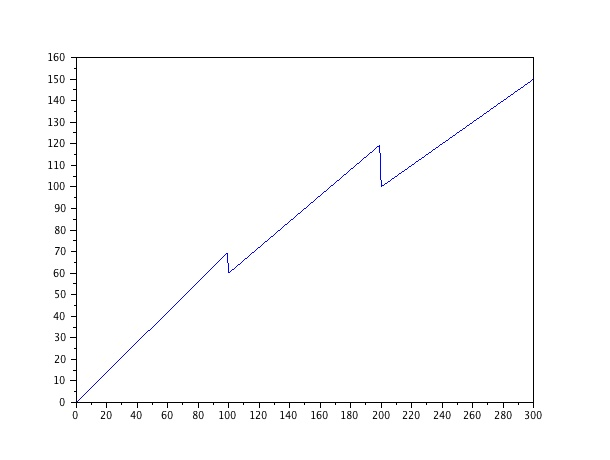
\includegraphics[width=0.7\textwidth]{figuren/verzamelingen_relaties/solden.jpeg}
\caption{Grafiek van de functie \texttt{bedrag}, getekend in Scilab.}
\label{fig:solden}
\end{figure}

Een algoritme kan ook \emph{recursief} zijn: uit de functiewaarde van het ene element leid je de functiewaarde van een ander element af. Voorbeeld hiervan is de functie die de waarde van $n!$ berekent. Immers $n!=n\cdot(n-1)!$. We verwijzen naar de OPO's `Algoritmen en datastructuren' voor meer details.



We vermelden tenslotte dat binaire relaties ook voorgesteld kunnen worden met grafen\footnote{\url{http://nl.wikipedia.org/wiki/Grafen}} en matrices\footnote{\url{http://nl.wikipedia.org/wiki/Matrix_(wiskunde)}}. Deze leerstof wordt behandeld in het OPO `Toegepaste Wiskunde 2'.

\section{Inverse relatie}
\label{sec:invrelatie}
Een relatie kan je `inverteren: je verwisselt bron en beeld met mekaar.
\begin{quote}
Zij $U$ een relatie van $A$ naar $B$: 
\[U=\{({x},{y})\mid {x}\in A \mathrm{~en~}{y}\in B\},\]
dan is de inverse relatie van $U$ gelijk aan 
\[U^{-1}=\{({y},{x})\mid ({x},{y})\in U \}\]
\end{quote}
Het komt erop neer dat je in de koppels $({x},{y})$ de $x$ en $y$ van plaats wisselt.


Is de inverse van een functie altijd opnieuw een functie?  In sectie~\ref{subsec:functies} gaven we aan dat een relatie een functie is waarbij elke $x$ hoogstens één beeld heeft. Neem de functie $f:\real\to\real:x\mapsto y= x^2$. Het getal \num{4} is beeld van zowel $x=2$ als $x=-2$. Voor de inverse functie moet je $x$ en $y$ met mekaar verwisselen, maar neem je dan 2 als invers beeld voor 4 of $-2$? We besluiten hieruit dat de inverse relatie van een functie niet altijd een functie is. Als de functie \emph{injectief} is, is de inverse van die functie wél een functie. 

Voorbeelden
\begin{itemize}
\item als $U$ de relatie `student $x$ heeft inschrijvingsnummer $y$', dan is de inverse relatie $U^{-1}$ de relatie `inschrijvingsnummer $y$ hoort bij student $x$'
\item als $V$ de relatie 'computer met serienummer $x$ is eigendom van persoon $y$', dan is de inverse relatie $V^{-1}$ de relatie 'persoon $y$ is eigenaar van computer met serienummer $x$'
\item gegeven de relatie $W=\{(x,y)\mid x,y\in \integers \mathrm{~en~} y=x+3\}$ dan is $W^{-1}=\{(a,b)\mid a,b\in \integers \mathrm{~en~} b=a-3\}$.
\end{itemize}




Als laatste bespreken we de inverse van een functie die omschreven wordt door een functievoorschrift. 
Neem het voorbeeld van de functie $f(x)=6+5\cdot x$ uit sectie~\ref{subsec:voorschrift} die het aantal gezwommen kilometers afbeeldt op het te betalen bedrag. De grafiek van deze functie wordt ook getoond in figuur~\ref{fig:fotos}. Op deze grafiek zie je duidelijk dat bij elke $x$ juist \'e\'en $y$ hoort. De functie is dus \'e\'en-op-\'e\'en en kan dus ge\"inverteerd worden. We moeten  de waarde van $x$ zoeken als we $y$ kennen. Als $y=20$, kunnen we op de grafiek aflezen dat $x\approx \num{2.8}$. Als je bij buurman \euros{20} sponsorgeld wil verdienen, moet je ongeveer \SI{2.8}{\kilo\meter} zwemmen. 

\begin{figure}[htbp]
\centering
\begin{tikzpicture}[x=2cm,y=0.25cm]
\draw[->] (-0.2,0) -- (5.2,0) node[right] {$x$};
\draw[->] (0,-1) -- (0,32) node[above] {$f(x)$};
\foreach \x in {0.5,1,...,5}
	\draw[shift={(\x,0)}] (0pt,2pt) -- (0pt,-2pt) node[below] {\footnotesize $\x$};
\foreach \y in {5,10,...,30}
	\draw[shift={(0,\y)},color=black] (2pt,0pt) -- (-2pt,0pt) node[left] {\footnotesize $\y$};
\draw[thick](0,6) -- (5,31);
\node [below left] at (0,0) {\footnotesize 0};
\draw[dashed,-latex](0,20) -- (2.8,20);
\draw[dashed, -latex](2.8,20) -- (2.8,0);
\filldraw [red] (2.8,20) circle (2pt);
\end{tikzpicture}
\caption{Grafiek van de functie $f(x)=6+5\cdot x$ }
\label{fig:fotos}
\end{figure}

Wil je exact weten hoeveel kilometer je moet zwemmen om \euros{20} te krijgen van buurman, kan je het functievoorschrift gebruiken:
\[
\begin{split}
y&=6+5\cdot x\\
& \Updownarrow\\
x&=\frac{y-6}{5}
\end{split}
\]
Als buurman \euros{20} betaalt, heb je $x=\frac{20-6}{5}=\frac{14}{5}=2,8$ kilometer gezwommen.







\newpage
\section{Oefeningen}
\begin{oef}
\label{oef21}
$A = \{1, 3, 5, 7\}$ en  $B = \{2, 4, 6,8\}$. Noteer volgende relaties door middel van opsomming:
\begin{enumerate}
\item $U=\{(x,y) \mid x\in A \mathrm{~en~} y \in B \mathrm{~en~} x+y<9\}$
\item $V=\{(x,y) \mid x\in A \mathrm{~en~} y \in B  \mathrm{~en~} x<y \}$
\end{enumerate}
\begin{opl}
\begin{enumerate}
\item $U=\{(1,2),(1,4),(1,6),(3,2),(3,4),(5,2) \}$
\item $V=\{(1,2),(1,4),(1,6),(1,8),(3,4),(3,6),(3,8),(5,6),(5,8),(7,8) \}$
\end{enumerate}
\end{opl}
\end{oef}

\begin{oef}
\begin{enumerate}
\item Bepaal domein en bereik van de relaties van oefening~2.1.
\item Geef de meest correcte benaming van de relaties.
\end{enumerate}
\begin{opl}
\begin{enumerate}
\item $\dom{U}=\{1,3,5 \}$; $\range{U}=\{2,4,6 \}$; relatie, geen injectie (want bvb. in het element 2 komen drie pijlen toe) of surjectie (want in het element 8 komt geen pijl toe). De relatie is geen functie want er zijn elementen met meer dan één beeld (bvb. het element 1 heeft drie beelden).
\item $\dom{V}=\{1,3,5,7 \}$; $\range{V}=\{2,4,6,8 \}$; surjectieve relatie
\end{enumerate}
\end{opl}
\end{oef}




\begin{oef}
Gegeven $X = \{\mathrm{a},\mathrm{ b}\}$ en $Y = \{\mathrm{c}, \mathrm{d}, \mathrm{e}, \mathrm{f}\}$. Noteer volgende productverzamelingen door middel van opsomming:
\begin{enumerate}
\item $X\times Y$
\item $Y\times X$
\item $X^2$
\end{enumerate}
\begin{opl}
\begin{enumerate}
\item $X\times Y=\{(a,c),(a,d),(a,e),(a,f),(b,c),(b,d),(b,e),(b,f) \}$
\item $Y\times X=\{(c,a),(c,b),(d,a),(d,b),(e,a),(e,b),(f,a),(f,b) \}$
\item $X^2=\{(a,a),(a,b),(b,a),(b,b) \}$
\end{enumerate}
\end{opl}
\end{oef}

\begin{oef}
Een e-mailadres kan je beschouwen als  een productverzameling van drie verzamelingen. Noteer deze verzamelingen zorgvuldig en definieer de gevraagde productverzameling.
\begin{opl}
$A=\{\text{strings bestaande uit a-zA-Z,.,0-9} \}$\\
$B=\{\text{strings bestaande uit a-zA-Z,.} \}$\\
$C=\{ \text{strings uit de lijst met goedgekeurde TLD's (Top Level Domain names}\}$\\
$A\times B\times C$
\end{opl}
\end{oef}

\begin{oef}
Hieronder vind je een aantal relaties van verzameling $A$ naar $B$. 
\begin{itemize}
\item Definieer voor elk van de gevallen de verzamelingen $A$ en $B$ eenduidig. Er zijn verschillende mogelijkheden.
\item Zoek een gepaste voorstellingswijze voor de relatie
\item Bepaal  welk soort relatie er beschreven wordt.
\end{itemize}
\begin{enumerate}
\item Klant heeft contactmoment
\item Klant heeft id
\item Persoon woont op adres
\item Student heeft telefoonnummer
\item Student krijgt rapport
\item Student volgt OPO
\end{enumerate}
\begin{opl}
\begin{enumerate}

\item Klant heeft contactmoment: $A$=$\{\text{klanten van het bedrijf}\}$; \\
$B=\{\text{mogelijke contactmomenten voor manager}\}$; 
één klant kan meerdere contactmomenten hebben, maar is er niet toe verplicht; 
niet alle mogelijke contactmomenten moeten ingevuld worden, maar nooit meer dan één klant per contactmoment: injectieve relatie

\item Klant heeft id: $A$=$\{\text{klanten van het bedrijf}\}$; \\
$B=\{\text{id's die de software toegekend heeft}\}$ 
iedere klant heeft juist één id: bijectie (afbeelding die bijectief is)

\item Persoon woont op adres: $A=\{\text{mensen met een geregistreerd adres}\}$; \\
$B=\{\text{geregistreerde adressen}\}$; iedere persoon woont op één adres; op één adres kunnen meerdere personen wonen: surjectie (afbeelding die surjectief is); als $A$ ook daklozen bevat: surjectieve functie

\item Student heeft telefoonnummer: $A=\{\text{studenten KHLeuven}\}$; \\
$B=\{$telefoonnummers die in het studentenregistratiesysteem opgenomen zijn$\}$.  Iedere student heeft nul, één of meerdere telefoonnummers; ieder telefoonnummer heeft één eigenaar: bijectieve relatie.
Als je broers en zussen toelaat als student: surjectieve relatie want telefoonnummer kan horen bij verschillende studenten.

\item Student krijgt rapport: $A=\{\text{leerlingen van KHLeuven}\}$; \\
$B=\{\text{afgedrukte rapporten op het einde van een examenperiode}\}$ voor elke student is er juist één rapport: bijectie (afbeelding die bijectief is)

\item Student volgt OPO: $A=\{\text{studenten van KHLeuven}\}$; \\
$B=\{\text{OPO's die de KHLeuven inricht}\}$ student volgt meerdere OPO's en elk OPO wordt door meerdere studenten gevolgd: surjectieve relatie, tenzij er OPO's zijn die door geen enkele student gevolgd worden (dat zou kunnen gebeuren bij keuzeOPO's bvb). In dat geval is het een gewone relatie.
\end{enumerate}

\end{opl}
\end{oef}

\begin{oef}
\label{oef:26}
Definieer volgende relaties correct:
\begin{itemize}
\item Bepaal bron- en doelverzameling zodat de relatie een bijectie is.
\item Stel de relatie voor als een verzameling van paren door middel van een functievoorschrift, bijv.\ $U=\{(x,y)|x,y\in \real\text{ en } y=x+1\}$
\item Geef nog minstens één andere voorstellingswijze
\end{itemize}
\begin{enumerate}
\item de functie $y=\sqrt{x}$
\item de relatie die de kostprijs van de brandstof van een autorit weergeeft in functie van de lengte van de rit (uitgedrukt in kilometers). De auto verbruikt \SI{6,45}{\litre} per \SI{100}{\kilo\meter}. De brandstof kost \euros{1,315} per liter.
\item de relatie die de prijs van de factuur van een mazoutlevering weergeeft in functie van het aantal gekochte liter. Mazout kost \euros{0,9155} per liter als je minder dan \SI{2000}{\litre} afneemt en \euros{0,8887} per liter als je meer dan \SI{2000}{\litre} afneemt.
\end{enumerate}
\begin{opl}
\begin{enumerate}
\item 
\begin{enumerate}
\item bron- en beeldverzameling: $\real^+$
\item $U=\{(x,y)|x,y\in \real^+\text{ en } y=\sqrt{x} \}$
\item zie figuur~\ref{oef:opl26}
\begin{figure}[htbp]
\centering
\begin{tikzpicture}[x=1cm,y=1cm]
\draw[help lines] (-1,-1) grid (9,4);
\draw[->] (-1.5,0) -- (9.5,0) node[right] {$x$};
\draw[->] (0,-1.5) -- (0,4.5) node[above] {$y$};
\foreach \x in {-1,1,2,...,9}
	\draw[shift={(\x,0)}] (0pt,2pt) -- (0pt,-2pt) node[below] {\footnotesize $\x$};
\foreach \y in {-1,1,2,...,4}
	\draw[shift={(0,\y)},color=black] (2pt,0pt) -- (-2pt,0pt) node[left] {\footnotesize $\y$};
\draw [domain=0:9,samples=200,thick] plot(\x,{sqrt(\x)});
\node [below left] at (0,0) {\footnotesize 0};
\end{tikzpicture}
%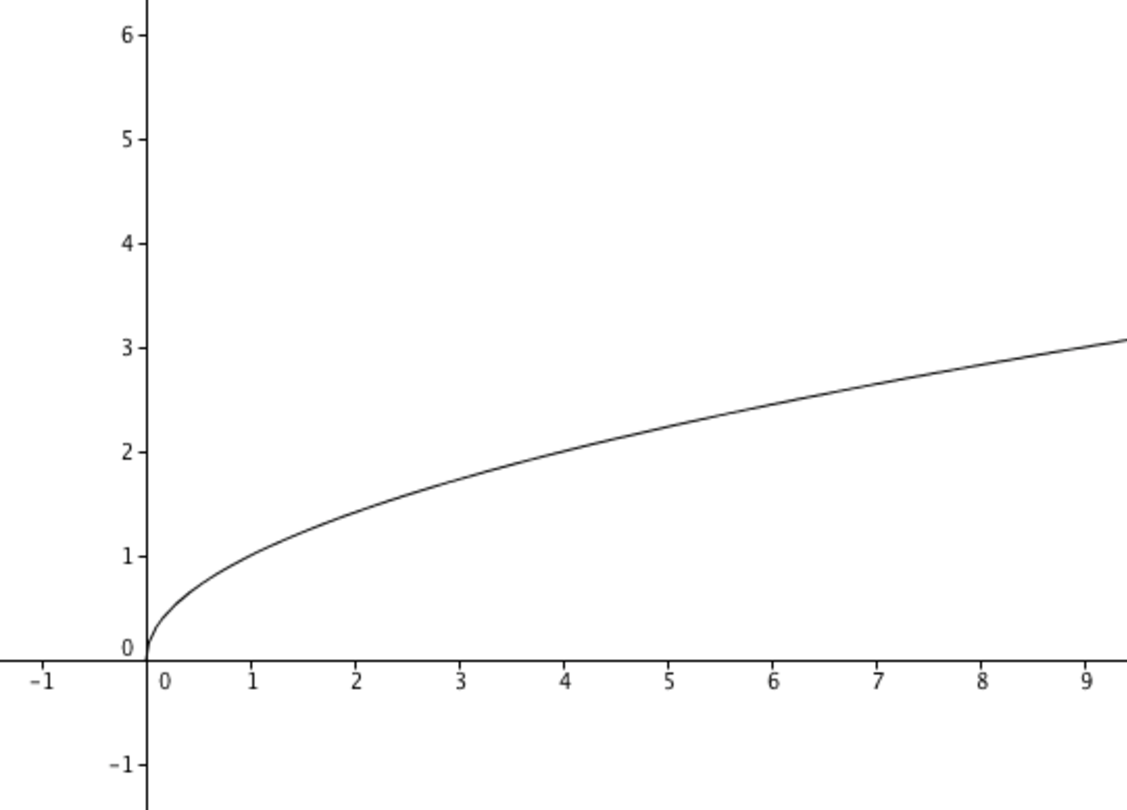
\includegraphics[width=0.5\textwidth]{figuren/verzamelingen_relaties/opl_oef26}
\caption{Oplossing van oefening~\ref{oef:26} }
\label{oef:opl26}
\end{figure}
\end{enumerate}


\item 
\begin{enumerate}
\item bron- en beeldverzameling is  $\real^+$
\item $U=\{(x,y)|x,y\in \real^+\text{ en } y=8,48175\cdot x/100\}$
\end{enumerate}
\item 
\begin{enumerate}
\item bron- en beeldverzameling is  $\real^+$
\item $U=\left\lbrace(x,y)\;|\;x,y\in \real^+\text{ en } y=
\begin{cases}
0,9155\cdot x&\text{ als }x<2000\\
0,8887\cdot x&\text{ anders }
\end{cases} \qquad
\right\rbrace$
\end{enumerate}

\end{enumerate}
\end{opl}
\end{oef}

\begin{oef}
Wat is de inverse van volgende relaties? Stel de relatie op dezelfde manier voor als de opgave.
\begin{enumerate}
\item $\{(1,7),(2,10),(3,9) \}$
\item 
\begin{tabular}{c|cccccc}
$x$ & \num{0.1} & \num{0.2} & \num{0.3} & \num{0.4} & \num{0.5} & \num{0.6} \\ 
\midrule
$y$ & 2 & 4 & 6 & 8 & 10 & 12 \\ 
\end{tabular} 
\item $f: \real\rightarrow\real:x\mapsto y \mid y=2\cdot x+10 $
\item $f: \real^+\rightarrow\real:x\mapsto y \mid y=\sqrt{x}$
\end{enumerate}
\begin{opl}
\item \{(7,1),(10,2),(9,3) \}
\item 
\begin{tabular}{c|cccccc}
$y$ & 2 & 4 & 6 & 8 & 10 & 12 \\ 
\midrule
$x$ & \num{0.1} & \num{0.2} & \num{0.3} & \num{0.4} & \num{0.5} & \num{0.6} \\ 
\end{tabular} 
\item $f^{-1}: \real\rightarrow\real:x\mapsto  y=\dfrac{x-10}{2} $
\item $f^{-1}: \real^+\rightarrow\real^+:x\mapsto y=x^2$
\end{opl}
\end{oef}

\begin{oef}
Zelfde vraag voor elke figuur:
\begin{itemize}
\item Teken de inverse functie.
\item Wat is het functievoorschrift van de getekende functie en zijn inverse?
\end{itemize}
\begin{enumerate}

\begin{minipage}{\columnwidth}
\item
%\centering
\begin{tikzpicture}[x=1cm,y=.5cm]
\draw[help lines] (-1,-2) grid (5,12);
\draw[->] (-1.5,0) -- (6,0) node[right] {$x$};
\draw[->] (0,-2) -- (0,13) node[above] {$y$};
\foreach \x in {-1,1,2,...,5}
	\draw[shift={(\x,0)}] (0pt,2pt) -- (0pt,-2pt) node[below] {\footnotesize $\x$};
\foreach \y in {-2,2,4,...,12}
	\draw[shift={(0,\y)},color=black] (2pt,0pt) -- (-2pt,0pt) node[left] {\footnotesize $\y$};
\draw[thick](5,-2.5) -- (-1,12.5); % rechte 1
\node [below left] at (0,0) {\footnotesize 0};
\end{tikzpicture}
\end{minipage}
%
%\item
%\centering
%\vspace{-0.4cm}
%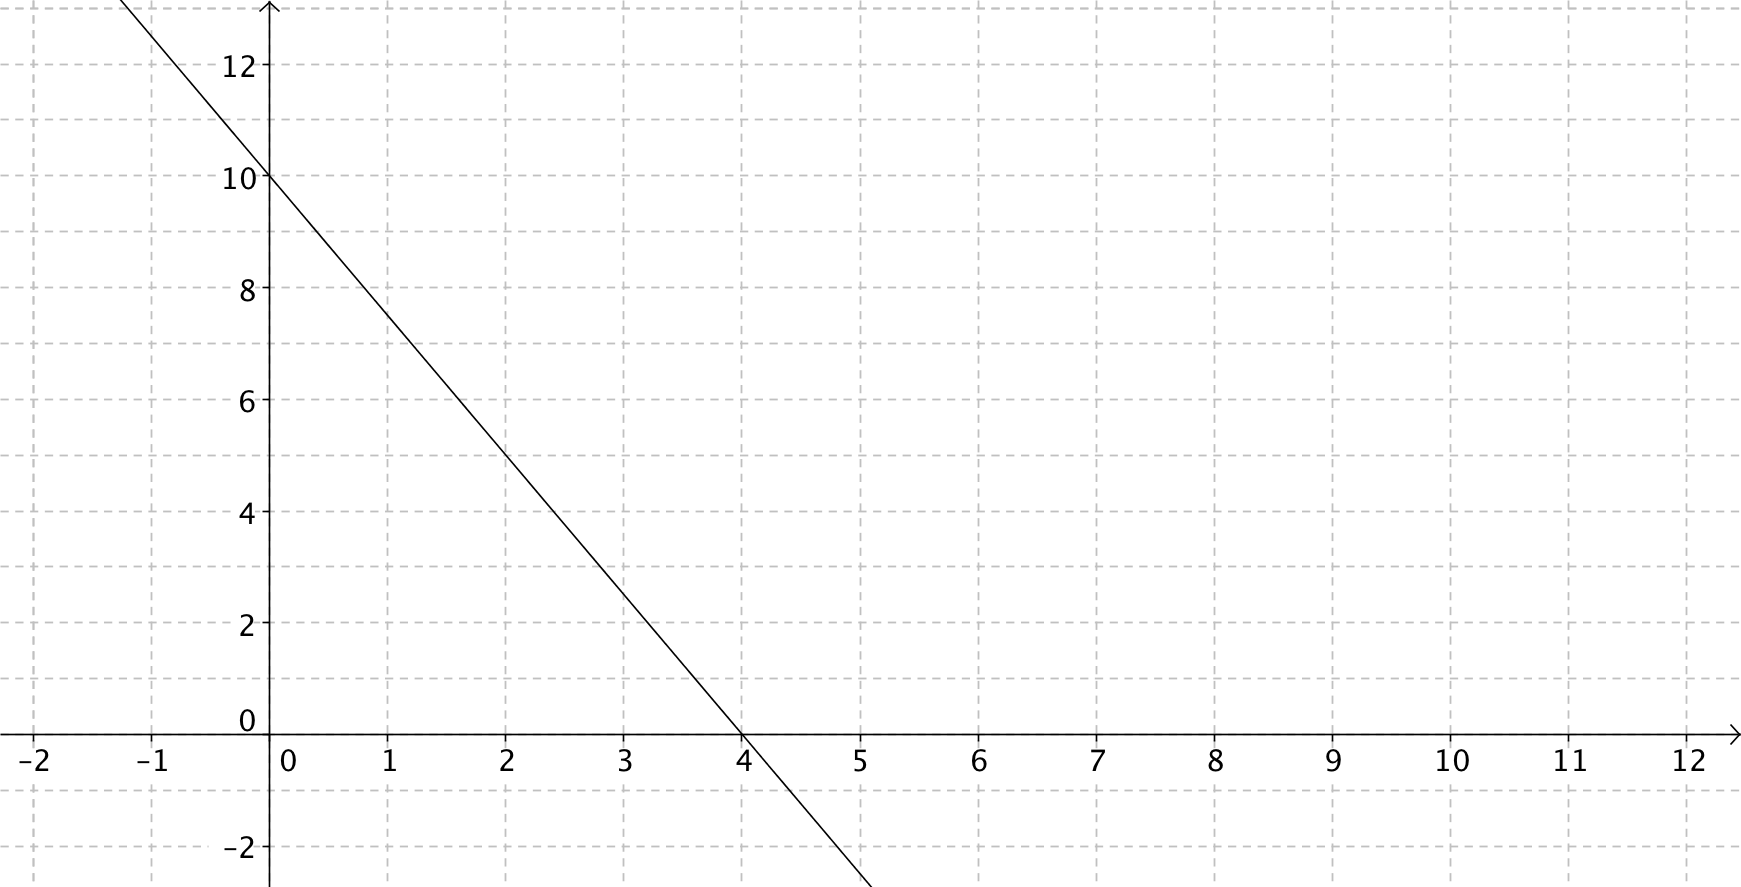
\includegraphics[width=0.7\textwidth]{figuren/verzamelingen_relaties/grafiek_lineair1}


\begin{minipage}{\columnwidth}
\item
%\centering
\begin{tikzpicture}[x=1cm,y=.2cm]
\draw[help lines] (-3,-11) grid (7,10);
\draw[->] (-3.5,0) -- (7.5,0) node[right] {$x$};
\draw[->] (0,-11) -- (0,12) node[above] {$y$};
\foreach \x in {-3,-2,-1,1,2,...,7}
	\draw[shift={(\x,0)}] (0pt,2pt) -- (0pt,-2pt) node[below] {\footnotesize $\x$};
\foreach \y in {-10,-5,5,10}
	\draw[shift={(0,\y)},color=black] (2pt,0pt) -- (-2pt,0pt) node[left] {\footnotesize $\y$};
\draw[thick](-3,-11) -- (7,9); % rechte 1
\node [below left] at (0,0) {\footnotesize 0};
\end{tikzpicture}
%\includegraphics[width=0.7\textwidth]{figuren/verzamelingen_relaties/grafiek_lineair2}
\end{minipage}

\begin{minipage}{\columnwidth}
\item
%\centering
\begin{tikzpicture}[x=1cm,y=.5cm]
\draw[help lines] (-7,-4) grid (4,4);
\draw[->] (-7.5,0) -- (4.5,0) node[right] {$x$};
\draw[->] (0,-4.5) -- (0,4.5) node[above] {$y$};
\foreach \x in {-7,-6,...,-1,1,2,...,4}
	\draw[shift={(\x,0)}] (0pt,2pt) -- (0pt,-2pt) node[below] {\footnotesize $\x$};
\foreach \y in {-4,-2,2,4}
	\draw[shift={(0,\y)},color=black] (2pt,0pt) -- (-2pt,0pt) node[left] {\footnotesize $\y$};
\draw[thick](-7,0.8) -- (4,-3.6); % rechte 1
\node [below left] at (0,0) {\footnotesize 0};
\end{tikzpicture}
%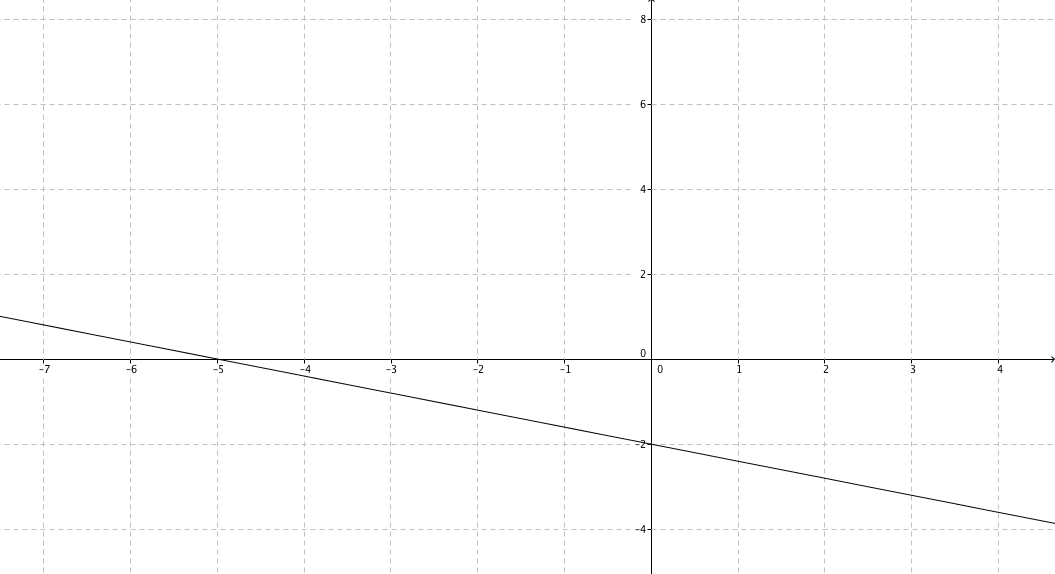
\includegraphics[width=0.7\textwidth]{figuren/verzamelingen_relaties/grafiek_lineair4}
\end{minipage}

\end{enumerate}

\begin{opl}
\begin{enumerate}
\item $y=-\frac52 x +10$; inverse functie: $y=-\frac25 x +4$
\item $y=2x-5$; inverse functie: $y=\frac12 x+\frac52$
\item $y=-\frac25x-2$; inverse functie: $y=-\frac52x-5$
\end{enumerate}
\end{opl}
\end{oef}

\begin{oef}
De volgende grafieken stellen relaties voor met als bron- en doelverzameling het interval $[0,1]$. Geef voor elk van de relaties aan of deze
functies, afbeeldingen, injectief, surjectief en/of bijectief zijn.
\begin{center}
  \newcommand{\axes}{
    \path[use as bounding box] (-.5,-.5) rectangle (4,4);
    \draw[step=3cm,gray,thin] (-.5,-.5) grid (4,4);
    \draw[thin,->] (-.5,0) -- (4,0);
    \draw[thin,->] (0,-.5) -- (0,4);
  }
  \begin{tabular}{cc}
    1.
    \begin{tikzpicture}
      \axes
      \draw[thick] (0,0) -- (3,3);
    \end{tikzpicture}
    &
    2.
    \begin{tikzpicture}
      \axes
      \draw[thick] (0,0) to[out=90,in=-90] (3,3);
    \end{tikzpicture}
    \\
    3.
    \begin{tikzpicture}
      \axes
      \draw[thick] (1.5,0) -- (1.5,3);
    \end{tikzpicture}
    &
    4.
    \begin{tikzpicture}
      \axes
      \draw[thick] (0,1.5) -- (3,1.5);
    \end{tikzpicture}
    \\
    5.
    \begin{tikzpicture}
      \axes
      \draw[thick] (0,0) to[out=45,in=180] (1,2) to[out=0,in=180] (2,1) to[out=0,in=225] (3,3);
    \end{tikzpicture}
    &
    6.
    \begin{tikzpicture}
      \axes
      \draw[thick] (1.5,1.5) circle (1cm);
    \end{tikzpicture}
  \end{tabular}
\end{center}
\begin{opl}
  \hspace{1mm}
  \begin{center}
    \begin{tabular}{cccccc}
      & \rotatebox{90}{functie}
      & \rotatebox{90}{afbeelding}
      & \rotatebox{90}{injectief}
      & \rotatebox{90}{surjectief}
      & \rotatebox{90}{bijectief} \\
      \toprule
      1. & \checkmark & \checkmark & \checkmark & \checkmark & \checkmark \\
      2. & \checkmark & \checkmark & \checkmark & \checkmark & \checkmark \\
      3. &            &            &            &            &            \\
      4. & \checkmark & \checkmark &            &            &            \\
      5. & \checkmark & \checkmark &            & \checkmark &            \\
      6. &            &            &            &            &            \\
    \end{tabular}
  \end{center}
\end{opl}
\end{oef}


%%% Local Variables: 
%%% mode: latex
%%% TeX-master: "cursusTW1"
%%% End: 

%%%%%%%%%%%%%%%%%%%%%%%%%%%%%%%%
%
% 6 sept 2013 [Jan]: lay-out verbeterd, kommagetallen, figuur iets verkleind, foutjes
%
%%%%%%%%%%%%%%%%%%%%%%%%%%%%%%%%%
\chapter{Eerstegraadsfuncties}
\label{chap:eerstegraadsfuncties}
\begin{quote}
     \textit{{\small `En hoeveel uur les hadden jullie per dag?' zei
     Alice, die vlug van onderwerp wilde veranderen.}}

     \textit{{\small `De eerste dag tien uur,' zei de Nepschildpad,
     `de volgende negen enzovoort.'}}

     \textit{{\small `Wat een raar lesrooster!' riep Alice uit.}}

     \textit{{\small `Zo lesten we onze dorst naar kennis steeds
     sneller,' merkte de Griffioen op, `vandaar de uitdrukking ''lest
     best''.'}}

     \textit{{\small Dat was volkomen nieuw voor Alice en ze dacht er
     even over na voordat ze haar volgende opmerking maakte. `Dus
     hadden jullie de elfde dag vrij?'}}

     \textit{{\small `Reken maar,' zei de Nepschildpad.}}

     \textit{{\small `En wat deden jullie met de twaalfde dag?' vroeg
     Alice gretig verder.}}

          Uit `Alice in Wonderland' -- Lewis Carroll
\end{quote}


\newpage
\noindent Veel verbanden tussen grootheden (snelheid, prijs, massa, lengte, aantal \ldots) kunnen voorgesteld worden door een veeltermfunctie van de eerste graad, kortweg \emph{eerstegraadsfunctie}\index{eerstegraadsfunctie}\footnote{Een veelterm van de eerste graad in de veranderlijke $x$ heeft de vorm $a+bx$. Er staat enkel een $x$ (tot de eerste macht) en dus spreken we over `\ldots van de eerste graad'.}. De grafiek hiervan is een rechte. Verder in de cursus maken we geregeld gebruik van eerstegraadsfuncties en rechten (bvb. lineaire programmatie, lineaire groei, rekenkundige rijen). We verwachten dus dat je vlot kan werken met dit type functie. Deze leerstof zag je reeds in het secundair, maar waarschijnlijk kan een herhaling geen kwaad?

\section{Hoeveel kost een taxirit?}\label{sec:taxirit}
Je plant een uitstapje naar Brussel. Alle verplaatsingen in Brussel zelf doe je met een taxi. 
 \begin{figure}[htbp]
      \centering
     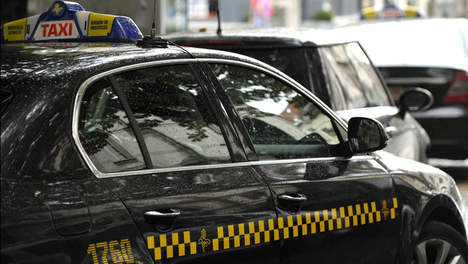
\includegraphics[width=\textwidth]{figuren/eerstegraadsfuncties/taxi.jpg}
     \caption{Nieuwe zwartgele Brusselse taxi}
     \label{fig:taxi}
 \end{figure}
Het zou fijn zijn om op voorhand een schatting van de kostprijs te kunnen maken. Op de site van mobielbrussel\footnote{\url{http://www.mobielbrussel.irisnet.be/articles/taxi/hoeveel-kost-een-taxi}} vind je volgende informatie:
\begin{itemize}
\item Instapgeld: \euros{2,40}
\item Tarief I (in de 19 gemeenten van het Brussels Hoofdstedelijk Gewest): \euros{1,80} per km.
\item Tarief II (buiten de 19 gemeenten): \euros{2,70} per km.
\item Wachtvergoeding: \euros{30} per uur.
\item Tussen 22 en 6 uur wordt een forfaitaire meerprijs van \euros{2,00} gevraagd.
\end{itemize}
Hoeveel kost een ritje van 15 km in het centrum om middernacht?  Hoever geraak je 's nachts in het centrum met \euros{20}? 

Om deze vragen te beantwoorden stellen we een \emph{wiskundig model} op. In dit geval gaat het om een eenvoudig model. Het verband tussen de afstand en de kostprijs kan beschreven worden door een lineair model. De bijbehorende functie is een veeltermfunctie van de eerste graad, kortweg `eerstegraadsfunctie' genoemd.

In dit model houden we geen rekening met opstoppingen (en is er dus geen wachtvergoeding) en gaan we uit van een teller die continu doorloopt en per meter registreert (en dus niet per km pas verspringt). Als je nu luidkeels protesteert en het niet eens bent met deze veronderstellingen, heb je natuurlijk groot gelijk. Een taximeter gaat inderdaad met sprongetjes vooruit! We komen hierop in \cref{sec:taxisprong} op pagina~\pageref{sec:taxisprong} terug en bekijken hoe we het model dan kunnen aanpassen. 

\section{Op zoek naar de functie}
In deze sectie gaan we op zoek naar een wiskundig model dat ons de prijs kan geven voor een bepaalde afstand in het centrum 's nachts.
Uit het algemeen hoofdstuk over functies weet je nog dat er verschillende manieren zijn om een functie voor te stellen:
\begin{itemize}
\item een tabel met getallen en bijhorende functiewaarden;
\item een grafiek;
\item een wiskundig voorschrift.
\end{itemize}

\subsection{Enkele functiewaarden berekenen}
Meestal is het een goed idee om te beginnen met enkele \emph{concrete afstanden} de kostprijs te noteren/berekenen en de gevonden waarden te noteren in een tabel. Om alles wat korter te noteren voeren we enkele notaties in. De afstand in km noemen we $x$. Voor de kostprijs in \euro \ gebruiken we $P$. Aangezien er bij elke afstand $x$ juist één kostprijs $P$ hoort is dit verband zeker een functie en mogen we $P(x)$ schrijven.

Gewoon instappen in een taxi (en 0 km rijden) kost op zich al geld. Je betaalt \euros{4,40} aan instapgeld en het nachtforfait. Wiskundig noteren we $P(0)=4,40$.

Als je 1 km rijdt komt er \euros{1,66} bij. Het totale bedrag voor een rit van 1 km is $P(1)=4,40+1,66=6,06$. Nog een km verder is er terug hetzelfde bedrag bijgekomen en wordt de totale kostprijs $P(2)=P(1)+1,66=7,72$. Deze berekening een aantal keer herhalen levert \cref{tbl:taxi}

\begin{table}[htbp]
    \centering
    \caption{Prijs van een taxirit i.f.v. de afstand}
    \begin{tabular}{SSp{2cm}SS}
    \toprule
    {Afstand} & {Kostprijs} & & {Afstand} & {Kostprijs} \\
    \midrule
0 & 4,40 & & 9 & 19,34 \\
1 & 6,06  & & 10 & 21 \\
2 & 7,72 & & 11 & 22,66 \\
3 & 9,38  & & 12 & 24,32 \\
4 & 11,04 & & 13 & 25,98 \\
5 & 12,7 & &14 & 27,64 \\
6 & 14,36 & & 15 & 29,3 \\
7 & 16,02 & & 16 & 30,96 \\
8 & 17,68  & & & \\
    \bottomrule
     \end{tabular}
    \label{tbl:taxi}
\end{table}

We hadden hierboven twee vragen: hoeveel kost een nachtelijke rit van 15 km en hoever geraak je met \euros{20}?
De eerste vraag is eenvoudig op te lossen met de tabel: je zoekt de afstand 15 op in de kolom `Afstand' en
leest op dezelfde rij de prijs af in de `Kostprijs' kolom, nl.\ \euros{29,30}.

De tweede vraag is iets moeilijker. Hoever geraak je met \euros{20}? Hiervoor moeten
we in de prijskolom 20 opzoeken, maar dat staat er niet tussen.
Met behulp van deze tabel kunnen we wel besluiten dat we ergens tussen 9 en \SI{10}{\km} halen. 

\subsection{Een grafische voorstelling}
\label{subsec:grafischeVoorstelling}
We zetten de punten uit \cref{tbl:taxi} in een grafiek.
\emph{Denk even na over de grootte van de assen vooraleer je een figuur maakt.}
Hier lijkt een $x$-as tot 16 en een $y$-as tot 31 aangewezen. Alle punten uit de tabel liggen op \cref{fig:taxir} op \'e\'en rechte.
\begin{figure}[htbp]
    \centering
\begin{tikzpicture}[x=0.5cm,y=0.25cm]
\draw[->] (-1,0) -- (17,0) node[right] {$x$};
\draw[->] (0,-1) -- (0,32) node[above] {$P$};
\foreach \x in {1,2,4,...,15,16}
	\draw[shift={(\x,0)}] (0pt,2pt) -- (0pt,-2pt) node[below] {\footnotesize $\x$};
\foreach \y in {5,10,...,30}
	\draw[shift={(0,\y)},color=black] (2pt,0pt) -- (-2pt,0pt) node[left] {\footnotesize $\y$};
\draw[thick](0,4.5) -- (16,30.96);
\node [below left] at (0,0) {\footnotesize 0};
\filldraw [red] (15,29.3) circle (2pt);
\filldraw [red] (3,9.38) circle (2pt) node[below right] {(3;9,38)};
\filldraw [red] (1,6.06) circle (2pt) node[below right] {(1;6,06)};
\filldraw [red] (8,17.68) circle (2pt) node[below right] {(8;17,68)};
\draw[dashed,-latex](15,0) -- (15,29.3);
\draw[dashed, -latex](15,29.3) -- (0,29.3);
\draw[dashdotted,-latex](0,20) -- (9.397,20);
\draw[dashdotted, -latex](9.397,20) -- (9.397,0);
\end{tikzpicture}
\caption{Prijs $P(x)$ van een taxirit i.f.v. de afstand $x$}
    \label{fig:taxir}
\end{figure}

We kunnen beide vragen nu ook \emph{grafisch} oplossen. Hoeveel kost een rit van 15 km? Teken een verticale (streepjeslijn) bij $x=15$. Deze verticale snijdt de rechte. Door het snijpunt teken je een horizontale. Die snijdt de verticale $P$-as net onder 30. De juiste waarde is op deze figuur niet af te lezen, maar dat is \emph{meestal ook niet de bedoeling van een grafische voorstelling}.

Omgekeerd vroegen we ons af hoever we geraakten met \euros{20}? Vertrek nu van 20 op de $P$-as met een horizontale rechte (punt-streepjeslijn). Door het snijpunt met de prijsrechte komt een verticale rechte. Die snijdt de $x$-as ergens tussen 9 en 10. Opnieuw is de exacte waarde niet af te lezen op de grafiek.



\subsection{Een formule}
Om exacte waarden te berekenen is een voorschrift, een formule vaak de aangewezen voorstellingsvorm voor een functie. We redeneren als volgt: per extra km komt er \euros{1,66} bij. Dit geeft volgende berekeningen:
\begin{align*}
P(0)&=4,40\\
P(1)&=P(0)+1,66=4,40+1,66=6,06\\
P(\mathbf{2})&=P(1)+1,66=4,40+\mathbf{2}\cdot 1,66=7,72\\
P(\mathbf{3})&=P(2)+1,66=4,40+\mathbf{3}\cdot 1,66= 9,38\\
\ldots \ &=\ \ldots \\
P(x)&=4,40+x\cdot 1,66
\end{align*}
Formule~\ref{eq:taxi} geeft bijgevolg het verband tussen de afstand $x$ en de kostprijs $P$. Het is een veeltermfunctie van de eerste graad, kortweg `eerstegraadsfunctie' of `lineaire functie' genoemd.
\begin{equation}\label{eq:taxi}
P(x)=1,66\cdot x + 4,40
\end{equation}
Deze formule laat ons nu toe om het antwoord op bovenstaande vragen via rekenwerk op te lossen. Hoeveel kost een rit van 15 km? Vul $x=15$ in formule~\eqref{eq:taxi} in:
\[
P(15)=1,66\cdot 15 + 4,40=29,30.
\]
Deze rit kost dus \euros{29,30}.

De omgekeerde vraag vergt iets meer werk. Hoever geraak je met \euros{20}? Merk op dat we nu de prijs $P$ krijgen en dat men de afstand $x$ vraagt. De prijs invullen levert een vergelijking in de onbekende $x$, die je oplost volgens de regels van de algebra:
\begin{align*}
20&=1,66\cdot x + 4,40\\
\Leftrightarrow 20-4,40&=1,66 \cdot x\\
\Leftrightarrow \dfrac{15,60}{1,66}&=x\\
\Leftrightarrow 9,3976 &= x
\end{align*}
Met \euros{20} geraken we dus 9,4 km (afgerond) ver.

\section{Richtingscoëfficiënt}
\subsection{Inleiding}
We hernemen \cref{fig:taxir} in \cref{fig:taxiredetail}.
\begin{figure}[htbp]
    \centering
\begin{tikzpicture}[x=1.8cm,y=0.8cm]
\draw[->] (-0.5,0) -- (4.5,0) node[right] {$x$};
\draw[->] (0,-0.5) -- (0,11.5) node[above] {$P$};
\foreach \x in {1,...,4}
	\draw[shift={(\x,0)}] (0pt,2pt) -- (0pt,-2pt) node[below] {\footnotesize $\x$};
\foreach \y in {1,...,11}
	\draw[shift={(0,\y)},color=black] (2pt,0pt) -- (-2pt,0pt) node[left] {\footnotesize $\y$};
\draw[thick](0,4.4) -- (4.1,11.206);
\node [below left] at (0,0) {\footnotesize 0};
\filldraw [red] (0,4.4) circle (2pt) ;
\filldraw [red] (3,9.38) circle (2pt) ;
\filldraw [red] (1,6.06) circle (2pt) ;
\filldraw [red] (2,7.72) circle (2pt) ;
\filldraw [red] (4,11.04) circle (2pt) ;
\draw[thick,donkergroen,-latex](0,4.4) -- (1,4.4) node[midway,above] {$+1$};
\draw[thick,blue,-latex](1,4.4) -- (1,6.06) node[midway,right] {$+1,66$};
\draw[thick,donkergroen,-latex](1,6.06) -- (2,6.06) node[midway,above] {$+1$};
\draw[thick,blue,-latex](2,6.06) -- (2,7.72) node[midway,right] {$+1,66$};
\draw[thick,donkergroen,-latex](2,7.72) -- (3,7.72) node[midway,above] {$+1$};
\draw[thick,blue,-latex](3,7.72) -- (3,9.38) node[midway,right] {$+1,66$};
\end{tikzpicture}
\caption{Rechte heeft rico 1,66}
    \label{fig:taxiredetail}
\end{figure}
\Cref{fig:taxiredetail} toont het belang van het getal 1,66. Per gereden km komt er \euros{1,66} bij de prijs bij. Als je op de grafiek in een punt van de rechte vertrekt en je tekent een horizontale rechte met lengte 1, dan is de lengte van het lijnstukje dat je verticaal naar boven moet gaan om terug op de rechte uit te komen gelijk aan 1,66. Deze afstand 1,66 wordt de \emph{richtingscoëfficiënt}\index{richtingsco\"effici\"ent}\index{rico} van de rechte genoemd (kortweg: \emph{rico}). 

\subsection{Berekening}
Gegeven een rechte door twee gegeven punten $(x_1, y_1)$ en $(x_2,y_2)$. De rico is dan
\begin{equation}\label{eq:rico}
\text{rico}=\dfrac{\text{\textcolor{blue}{verticale toename}}}{\text{\textcolor{donkergroen}{horizontale toename}}}=\dfrac{\textcolor{blue}{y_2-y_1}}{\textcolor{donkergroen}{x_2-x_1}}
\end{equation}
\begin{figure}[htbp]
    \centering
\begin{tikzpicture}[x=1cm,y=1cm]
\draw[->] (-0.5,0) -- (3.5,0) node[right] {$x$};
\draw[->] (0,-0.5) -- (0,4) node[above] {$y$};
\draw[shift={(1,0)}] (0pt,2pt) -- (0pt,-2pt) node[below] {\footnotesize $x_1$};
\draw[shift={(3,0)}] (0pt,2pt) -- (0pt,-2pt) node[below] {\footnotesize $x_2$};
	\draw[shift={(0,2)},color=black] (2pt,0pt) -- (-2pt,0pt) node[left] {\footnotesize $y_1$};
	\draw[shift={(0,3)},color=black] (2pt,0pt) -- (-2pt,0pt) node[left] {\footnotesize $y_2$};
\draw[thick](0.5,1.75) -- (3.5,3.25);
\node [below left] at (0,0) {\footnotesize 0};
\draw[dashed] (0,2) -| (1,0);
\draw[dashed] (0,3) -| (3,0);
\filldraw [red] (1,2) circle (2pt) ;
\filldraw [red] (3,3) circle (2pt) ;
\draw[thick,donkergroen,-latex](1,2) -- (3,2) node[midway,below] {$x_2-x_1$};
\draw[thick,blue,-latex](3,2) -- (3,3) node[midway,right] {$y_2-y_1$};
\end{tikzpicture}
\caption{Rico van rechte door twee punten}
    \label{fig:defrico}
\end{figure}
De rico van een rechte is dus volgens formule~\eqref{eq:rico} een breuk. De aandachtige lezer herinnert zich nog uit het secundair dat de noemer van een breuk nooit gelijk aan 0 mag worden. Dat is het geval als $x_2=x_1$, dus als beide punten op een verticale rechte liggen. We besluiten bijgevolg: \emph{de rico van een verticale rechte is niet gedefinieerd}.

\subsection{Stijgen en dalen}
De rico is een maat voor de toename van een grootheid als een andere grootheid toeneemt. Als ik 1 km met een taxi verder rijd, komt er \euros{1,66} bij de rekening bij. Een ritje buiten het centrum van Brussel kost \euros{2,70} per km zoals we zagen. De rechte die de prijs van zo'n taxirit weergeeft in functie van de afstand heeft dus een grotere rico. 

We kunnen voor de rico drie gevallen onderscheiden.

\subsubsection{Rico groter dan 0}
Een positieve rico komt overeen met een stijgende rechte. Hoe groter de rico, des te steiler stijgt de rechte. We spreken dan over een functie die een \emph{lineaire toename} kent.

\subsubsection{Rico kleiner dan 0}
Als de rico negatief is, daalt de functie. Het gaat hier dan om een functie die afneemt als de waarden op de horizontale as groter worden: \emph{lineaire afname}. 

\subsubsection{Rico gelijk aan 0}
De rico wordt 0 als $y_2-y_1=0$, dus als $y_2=y_1$. De twee punten liggen dan op een horizontale rechte. Er is geen toe- of afname meer. De functiewaarde is een \emph{constante} en hangt dus niet af van de waarde op de horizontale as. Alsof je in een taxi stapt die een vaste prijs heeft, hoe ver de rit ook is.

\section{Functievoorschrift}
\label{sec:functievoorschrift}
\subsection{Algemeen}
Algemeen ziet een lineaire functie er uit als
\begin{equation}\label{eq:linfunc}
f(x)=mx+q
\end{equation}
De coëfficiënt van $x$ (het getal $m$) vertelt iets over het stijgen en dalen van de rechte: de rico. Het getal $q$ is de $y$-waarde waarbij de rechte de verticale as snijdt. Immers, als we $x=0$ stellen in vergelijking~\eqref{eq:linfunc}:
\begin{align*}
f(0)&=m\cdot 0 + q\\
&= q
\end{align*}
Het getal $q$ is dus de functiewaarde in 0. Men noemt $q$ daarom soms ook de \emph{startwaarde}\index{startwaarde} van de functie, zeker als de veranderlijke op de horizontale as de tijd is.

We zullen in het vervolg van deze tekst de begrippen \emph{functievoorschrift} en \emph{vergelijking} door elkaar gebruiken. Het verschil is ondermeer dit: $f(x)=2x+3$ is het voorschrift van een eerstegraadsfunctie (of lineaire functie). Als we $f(x)$ vervangen door $y$ spreken we liever van een vergelijking van de rechte: $y=2x+3$. Vergelijkingen van rechten kunnen we bovendien algebraïsch aanpassen, bvb. $y-2x=3$ of $2x-y+3=0$ stelt telkens dezelfde rechte voor.

\subsection{Rechtevenredig verband}
Als in vergelijking~\eqref{eq:linfunc} de waarde van $q$ gelijk gesteld wordt aan 0, gaat de rechte door de oorsprong. De rechte krijgt dan als vergelijking $f(x)=mx$. We spreken dan over een \emph{rechtevenredig verband}\index{recht evenredig}.

Deze speciale eerstegraadsfunctie komt veel voor, bvb. 
\begin{itemize}
\item Bellen met een oplaadkaart: niet bellen kost \euros{0}. Vijf minuten bellen kost 5 keer zoveel als 1 minuut bellen. Het verband tussen de prijs en het aantal minuten is rechtevenredig.
\item Gehakt kopen bij een beenhouwer: als je \SI{0}{\gram} koopt kost het \euros{0}. Wie \SI{800}{\gram} gehakt koopt, betaalt 8 keer zoveel als iemand die \SI{100}{\gram} koopt.  Het verband tussen de prijs en de massa is rechtevenredig.
\end{itemize}

\section{De vergelijking van een rechte opstellen}
\Cref{fig:rechtevgl} toont een rechte. Hoe vind je het bijpassende functievoorschrift? We overlopen een aantal methodes die je in het derde jaar secundair in detail inoefende.
\begin{figure}[htbp]
    \centering
\begin{tikzpicture}[x=1cm,y=1cm]
\draw[help lines] (0,0) grid (5,4);
\draw[->] (-0.5,0) -- (5.5,0) node[right] {$x$};
\draw[->] (0,-0.5) -- (0,5) node[above] {$y$};
\foreach \x in {1,...,5}
	\draw[shift={(\x,0)}] (0pt,2pt) -- (0pt,-2pt) node[below] {\footnotesize $\x$};
\foreach \y in {1,...,4}
	\draw[shift={(0,\y)},color=black] (2pt,0pt) -- (-2pt,0pt) node[left] {\footnotesize $\y$};
\draw[thick](-0.5,4.25) -- (5.5,1.25);
\node [below left] at (0,0) {\footnotesize 0};

\end{tikzpicture}
\caption{Wat is de vergelijking van deze rechte?}
    \label{fig:rechtevgl}
\end{figure}

\subsection{Met snijpunt y-as en rico}
De rechte van \cref{fig:rechtevgl} snijdt de verticale as in het punt $(0,4)$ en dus is in vgl~\eqref{eq:linfunc} $q=4$. Met een kleine hulpconstructie (\cref{fig:rechtevgl2}) en formule~\eqref{eq:rico} vinden we als rico $m=\frac{-1}{2}$ (negatief want de rechte daalt). De gevraagde vergelijking wordt dus
\[
y=\frac{-1}{2}x+4
\]
en het functievoorschrift voor deze eerstegraadsfunctie is dus
\[
f(x)=\frac{-1}{2}x+4.
\]
\begin{figure}[htbp]
    \centering
\begin{tikzpicture}[x=1cm,y=1cm]
\draw[help lines] (0,0) grid (5,4);
\draw[->] (-0.5,0) -- (5.5,0) node[right] {$x$};
\draw[->] (0,-0.5) -- (0,5) node[above] {$y$};
\foreach \x in {1,...,5}
	\draw[shift={(\x,0)}] (0pt,2pt) -- (0pt,-2pt) node[below] {\footnotesize $\x$};
\foreach \y in {1,...,4}
	\draw[shift={(0,\y)},color=black] (2pt,0pt) -- (-2pt,0pt) node[left] {\footnotesize $\y$};
\draw[thick](-0.5,4.25) -- (5.5,1.25);
\node [below left] at (0,0) {\footnotesize 0};
\filldraw [red] (0,4) circle (2pt) ;
\filldraw [red] (2,3) circle (2pt) ;
\draw[thick,donkergroen,-latex](0,4) -- (2,4) node[midway,above] {$+2$};
\draw[thick,blue,-latex](2,4) -- (2,3) node[midway,right] {$-1$};
\end{tikzpicture}
\caption{Rico grafisch bepalen}
    \label{fig:rechtevgl2}
\end{figure}

\subsection{Eén punt en rico gegeven}
Stel dat je gegeven krijgt dat de rechte door het punt $(2,3)$ gaat en dat de rico gelijk is aan $-0,5$. Er zijn twee manieren om de vergelijking van deze rechte te vinden.

\subsubsection{Manier 1: punt invullen in algemene vergelijking}
Als de rechte een rico $-0,5$ heeft, dan heeft ze de algemene vorm $y=-0,5x+q$. Het snijpunt met de verticale as, $q$, kennen we niet. Het punt $(2,3)$ ligt op de rechte. \emph{`Liggen op'} betekent: \emph{`je mag dit punt invullen in de vergelijking'}. Invullen komt neer op $x$ vervangen door 2 en $y$ door 3. We bekomen 
\begin{align*}
3&=-0,5\cdot 2 + q\\
\Leftrightarrow 3&=-1+q\\
\Leftrightarrow 4&=q
\end{align*}
De gezochte vergelijking wordt dus: $y=-0,5x+4$.

\subsubsection{Manier 2: algemene formule gebruiken}
De vergelijking van een rechte door een gegeven punt $(x_1,y_1)$ met gegeven rico $m$ wordt gegeven door
\begin{equation}\label{eq:puntrico}
y-y_1=m(x-x_1).
\end{equation}
Formule~\eqref{eq:puntrico} uitrekenen voor het punt $(2,3)$ en rico $-0,5$ levert
\begin{align*}
y-3&=-0,5(x-2)\\
\Leftrightarrow y-3&=-0,5x + 1\\
\Leftrightarrow y&=-0,5x+4
\end{align*}

\subsection{Twee punten gegeven}
Dit kunnen we als een speciaal geval van formule~\eqref{eq:puntrico} zien. De vergelijking van een rechte door twee gegeven punten $(x_1,y_1)$ en $(x_2,y_2)$ wordt gegeven door
\begin{equation}\label{eq:puntpunt}
y-y_1=m(x-x_1) \quad \text{ met } \quad m=\dfrac{y_2-y_1}{x_2-x_1}.
\end{equation}

\section{Nulpunt van een lineaire functie}
Een nulpunt van een functie is een \emph{waarde waarvoor de functie gelijk wordt aan 0}. Grafisch komt dit neer op het zoeken van het \emph{snijpunt van de functiegrafiek met de horizontale as}. Om het nulpunt van een eerstegraadsfunctie te berekenen, los je een eerstegraadsvergelijking op.

Een voorbeeld: gegeven de functie $f(x)=-3x+5$. Het nulpunt is die $x$-waarde waarvoor $f(x)=0$, dus
\begin{align*}
0&=-3x+5\\
\Leftrightarrow 3x&=5\\
\Leftrightarrow x&=\dfrac{5}{3}
\end{align*}


\section{Snijpunt van twee rechten}
\Cref{fig:snijdenderechten} toont twee rechten met vergelijkingen $y=-x+5$ en $y=\frac{1}{2}x+1$. Met een stelsel zoek je het snijpunt van beide rechten. 
\begin{figure}[htbp]
    \centering
\begin{tikzpicture}[x=1cm,y=1cm]
\draw[help lines] (0,0) grid (5,5);
\draw[->] (-0.2,0) -- (6,0) node[right] {$x$};
\draw[->] (0,-0.2) -- (0,5.5) node[above] {$y$};
\foreach \x in {1,...,5}
	\draw[shift={(\x,0)}] (0pt,2pt) -- (0pt,-2pt) node[below] {\footnotesize $\x$};
\foreach \y in {1,...,5}
	\draw[shift={(0,\y)},color=black] (2pt,0pt) -- (-2pt,0pt) node[left] {\footnotesize $\y$};
\draw[thick](-0.2,5.2) -- (5.5,-0.5); % rechte 1
\draw[thick](-0.2,0.9) -- (5.5, 3.75);% rechte 2
\node [below left] at (0,0) {\footnotesize 0};
\filldraw [red] (2.67,2.33) circle (2pt) node[right=0.3cm] {$(\frac{8}{3},\frac{7}{3})$};
\draw[dashed](0,2.33) -| (2.67,0);
\end{tikzpicture}
\caption{Snijpunt van twee rechten}
    \label{fig:snijdenderechten}
\end{figure}

Er zijn verschillende methodes voor het oplossen van een stelsel van twee eerstegraadsvergelijkingen. Je herinnert je waarschijnlijk nog de \emph{substitutiemethode}\index{substitutiemethode}. Herschrijf één van beide vergelijkingen tot er staat `$\text{letter} = \ldots$'. Die letter vul je dan in (substitueren) in de andere vergelijking.

Hier zijn de vergelijkingen wel al in een eenvoudige vorm gegeven. We halen een letter uit één vergelijking: $y=-x+5$ (nogal evident, want de vergelijking staat al in de gewenste vorm). Die letter vul je in de andere vergelijking in:
\begin{align*}
y&=\frac{1}{2}x+1\\
\Leftrightarrow -x+5&=\frac{1}{2}x+1\\
\Leftrightarrow -x-\frac{1}{2}x&=-5+1\\
\Leftrightarrow -\frac{3}{2}x&=-4\\
\Leftrightarrow x&=\frac{8}{3}
\end{align*}

Deze waarde voor de onbekende $x$ vul je nu in in één van beide vergelijkingen: $y=-\frac{8}{3}+5=\frac{7}{3}$. Het snijpunt van beide rechten is dus $(\frac{8}{3},\frac{7}{3})$.

\section{Deelsgewijs lineaire functie}\label{sec:taxisprong}
\subsection{Definitie}
Soms kan een verband tussen twee grootheden voorgesteld worden door een aaneenschakeling van lineaire functies. We spreken in dit verband ook over functies met \emph{meervoudig voorschrift}\index{meervoudig voorschrift}. In algoritmes komt dit vaak voor: afhankelijk van de waarde van inputparameter(s) kunnen er verschillende berekeningen volgen (\verb+if ... then ... else ...+ constructies enz.).

Laten we even teruggrijpen naar het taxivoorbeeld (\cref{sec:taxirit}). We gingen ervan uit dat de meter `continu' doorloopt. Voor elke km, maar ook voor elke m, mm, \ldots \ loopt de prijs op. 

Dat is niet wat er in een echte taximeter gebeurt. Wie al een taxi nam, heeft gemerkt dat de meter `in sprongetjes' verhoogt. Laten we veronderstellen dat de taximeter per begonnen km een sprongetje maakt. We herhalen nog eens de getalwaarden: voor een rit in het centrum na 22 uur betaal je \euros{4,40} instapgeld en \euros{1,66} per \emph{begonnen} km. In deze veronderstelling maakt het niet uit of je nu 5,3 of 5,1 of 5,999 km rijdt. Deze drie afstanden kosten hetzelfde!

\subsection{Grafiek}
\Cref{fig:taxideels} toont de grafiek van de prijs van de taxirit in functie van de afstand in km. Aangezien de prijs gedurende een km constant blijft, bestaat de functie uit stukjes horizontale rechten. Met `open' en `gesloten' bolletjes duiden we aan welke waarde je moet kiezen in de grenspunten. Zo wijst het gesloten bolletje bij $(1;7,72)$ erop dat de functiewaarde $f(1)=7,72$.
\begin{figure}[htbp]
    \centering
\begin{tikzpicture}[x=1cm,y=1cm]
\draw[help lines] (0,0) grid (4.2,11.2);
\draw[->] (-0.1,0) -- (4.5,0) node[right] {$x$};
\draw[->] (0,-0.1) -- (0,11.3) node[above] {$P$};
\foreach \x in {1,...,4}
	\draw[shift={(\x,0)}] (0pt,2pt) -- (0pt,-2pt) node[below] {\footnotesize $\x$};
\foreach \y in {1,...,11}
	\draw[shift={(0,\y)},color=black] (2pt,0pt) -- (-2pt,0pt) node[left] {\footnotesize $\y$};
\node [below left] at (0,0) {\footnotesize 0};
%\filldraw [red] (15,29.3) circle (2pt);
%\filldraw [red] (3,9.38) circle (2pt) node[below right] {(3;9,38)};
%\filldraw [red] (1,6.06) circle (2pt) node[below right] {(1;6,06)};
%\filldraw [red] (8,17.68) circle (2pt) node[below right] {(8;17,68)};
\draw[thick] (0,6.06) -- (1,6.06);
\draw[thick] (1,7.72) -- (2,7.72);
\draw[thick] (2,9.38) -- (3,9.38);
\draw[thick] (3,11.04) -- (4,11.04);
\filldraw[fill=black, draw=black] (0,6.06) circle (2pt);
\filldraw[fill=white, draw=black] (1,6.06) circle (2pt);
\filldraw[fill=black, draw=black] (1,7.72) circle (2pt);
\filldraw[fill=white, draw=black] (2,7.72) circle (2pt);
\filldraw[fill=black, draw=black] (2,9.38) circle (2pt);
\filldraw[fill=white, draw=black] (3,9.38) circle (2pt);
\filldraw[fill=black, draw=black] (3,11.04) circle (2pt);
\filldraw[fill=white, draw=black] (4,11.04) circle (2pt);
\end{tikzpicture}
\caption{Deelsgewijs lineaire functie}
    \label{fig:taxideels}
\end{figure}

\subsection{Voorschrift}
Er zijn verschillende manieren om een voorschrift voor deze functie te geven. De eenvoudigste, maar langste, manier bestaat erin alle verschillende gevallen te beschrijven.
\begin{equation}
P(x)=\left\{
\begin{array}{ll}
6,06 &\text{ voor } x \in [0,1[ \\
7,72 &\text{ voor } x \in [1,2[ \\
9,38 &\text{ voor } x \in [2,3[ \\
\ldots &
\end{array}
\right.
\end{equation}

Voorschrift~\eqref{eq:taxifloor} is een stuk interessanter, maar ook wel een stuk moeilijker om te vinden.
\begin{equation}\label{eq:taxifloor}
P(x)= 1,66\cdot \mathtt{floor}(x+1)+4,40
\end{equation}
De functie $\mathtt{floor}(x)$ is het grootste geheel getal niet groter dan $x$. We gebruiken hier de notatie van Scilab (en veel andere programmeertalen). In wiskunde noteert men deze \verb+floor+-functie als $\lfloor x \rfloor$.

\section{Oefeningen}
\begin{oef}
De rechte $r$ gaat door punten $A$ en $B$. Stel het functievoorschrift op voor $r$. Zoek het nulpunt en het snijpunt met de verticale as.
\begin{enumerate}
\item $A(2,5)$ en $B(4,-1)$
\item $A(-2,-4)$ en $B(3,-4)$
\item $A(3,-1)$ en $B(3,6)$ 
\end{enumerate}
     \begin{opl}
\begin{enumerate}
\item $f(x)=-3x+11$, nulpunt $(\frac{11}{3}, 0)$ en snijpunt met de $y$-as: $(0,11)$
\item $f(x)=-4$, dus een constante functie. Deze functie heeft geen nulpunt en het snijpunt met de $y$-as is $(0,-4)$.
\item Deze rechte heeft als vergelijking $x=3$. Het is een verticale rechte en dus geen functie. Het heeft dan ook geen zin om te spreken over nulpunt en snijpunt met de $y$-as.
\end{enumerate}
     \end{opl}
\end{oef}

\begin{oef}
Figuur~\ref{fig:rechtenoef2} toont enkele rechten in een assenkruis. Stel een vergelijking op van de rechten. Welke stellen functies voor?
\begin{figure}[htbp]
    \centering
\begin{tikzpicture}[scale=0.8]
\draw[help lines] (-5,-5) grid  (5,5);
\draw[->] (-5.5,0) -- (5.5,0) node[right] {$x$};
\draw[->] (0,-5.5) -- (0,5.5) node[above] {$y$};
\foreach \x in {-5,...,-1,1,2,...,5}
	\draw[shift={(\x,0)}] (0pt,2pt) -- (0pt,-2pt) node[below] {\footnotesize $\x$};
\foreach \y in {-5,...,-1,1,2,...,5}
	\draw[shift={(0,\y)},color=black] (2pt,0pt) -- (-2pt,0pt) node[left] {\footnotesize $\y$};
\node [below left] at (0,0) {\footnotesize 0};
\draw[very thick] (-5,2.5) -- (5,-2.5) node[above] {$a$};
\draw[very thick] (-5,-4) -- (5,-4) node[above] {$b$};
\draw[very thick] (-5,-2) -- (2,5) node[above] {$c$};
\draw[very thick] (3,-5) -- (3,5) node[above] {$d$};
\end{tikzpicture}
\caption{Zoek een vergelijking voor deze rechten}
    \label{fig:rechtenoef2}
\end{figure}
\begin{opl} Enkel rechte $d$ is geen functie \\
$a\leftrightarrow y=-\frac{1}{2}x$\\
$b \leftrightarrow y=-4 $\\
$c \leftrightarrow y=x+3$\\
$d \leftrightarrow x=3$
\end{opl}
\end{oef}


\begin{oef}
Je twijfelt tussen drie verschillende tariefplannen voor telefonie. Je bent enkel geïnteresseerd in bellen (dus niet in SMS of data). Bij Proximus stelt men je het tarief `free call' voor. Echt `free' is het wel niet: je betaalt \euros{30} per maand, maar je mag wel onbeperkt bellen naar alle netwerken. Mobistar vertelt je dat hun tarief `olifant' het goedkoopste is. Je betaalt een abonnementskost van \euros{15}. Je mag dan wel een uur gratis bellen. Als je gratis uur opgebruikt is, worden je telefoongesprekken betalend tegen \euros{0,25} per minuut. Base beweert dat je nergens goedkoper belt dan met hun `simpel' herlaadkaart: geen abonnementskosten, enkel \euros{0,40} per belminuut.

Maak een figuur van de verschillende tarieven (kostprijs i.f.v. de beltijd). Duid op de figuur aan wat de goedkoopste formule is voor elke beltijd. Geef een overzichtelijk antwoord.

Stel dat je telkens voor de goedkoopste formule gaat. Hoeveel kosten dan respectievelijk 10, 100 en 1000 belminuten?
\begin{opl}
Tot een maandelijkse beltijd van 37,5 minuten is Base het goedkoopst. Tussen 37,5 en 120 minuten kan je best Mobistarklant worden. Voor wie meer belt dan twee uur per maand is Proximus het goedkoopst. 
Voor 10 belminuten kies je dus Base met een kostprijs van $10\cdot 0,40=4$ euro. Als je 100 minuten per maand belt, ben je goedkoopst bij Mobistar. Dat kost je dan \euros{25}. Wie 1000 minuten belt, hoeft niet te twijfelen: kies Proximus en dus kost het je \euros{30}.
\end{opl}
\end{oef}

\begin{oef}
De snelste supercomputer (figuur~\ref{fig:ibmBG}) in 2012 is de IBM Blue Gene Sequoia\footnote{\url{http://www.top500.org/list/2012/06/100}}.  Deze computer haalt 16324 TFlops (Teraflops). 
\begin{figure}[hbtp]
\centering
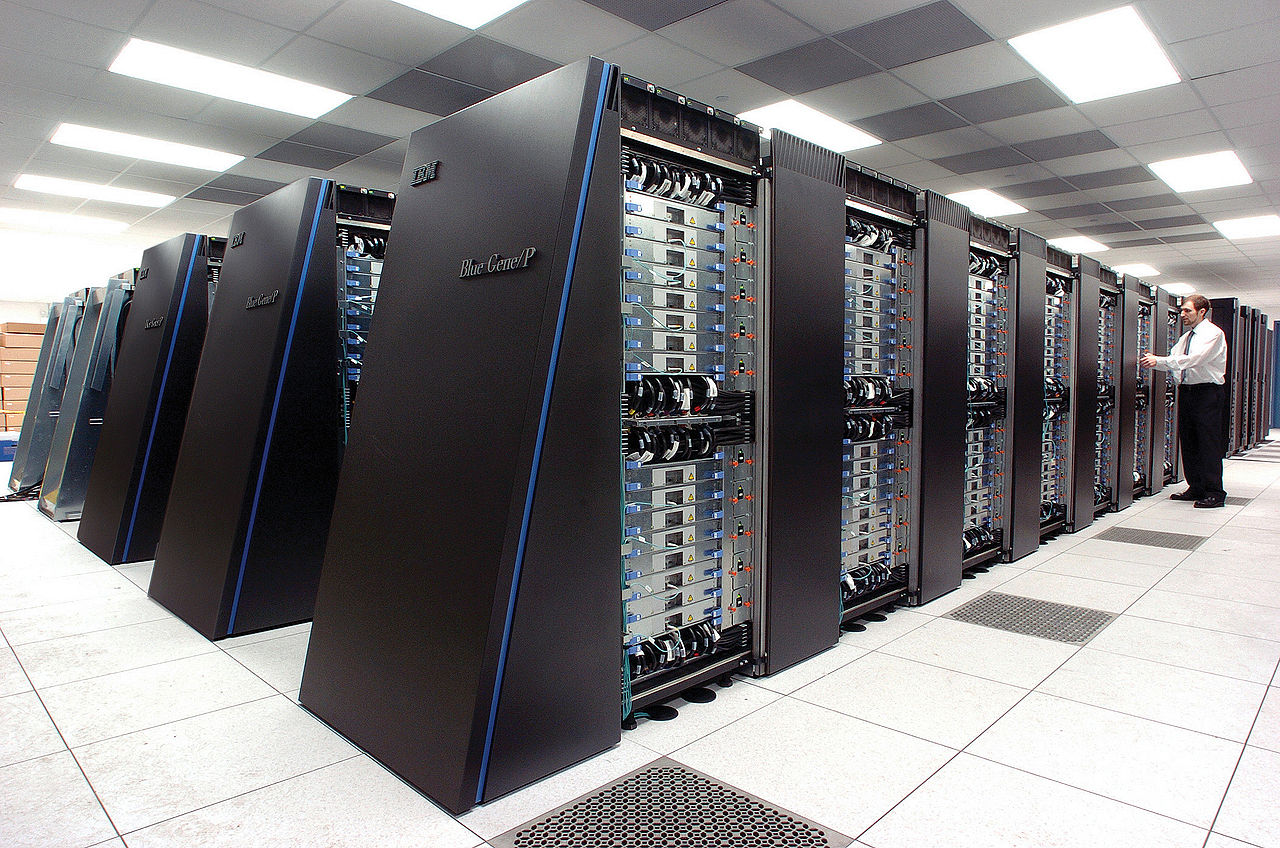
\includegraphics[width=\textwidth]{figuren/eerstegraadsfuncties/IBMBlueGene.jpg}
\caption{IBM Blue Gene supercomputer}
\label{fig:ibmBG}
\end{figure}

Eén teraflop is $10^{12}$ floating point berekeningen per seconde. Het vermogen bedraagt \SI{7,890}{\mega\watt}. Ter vergelijking: de grootste kerncentrale in Doel (4) heeft een vermogen van ongeveer \SI{1000}{\mega\watt}, wat betekent dat ongeveer 126 van dergelijke supercomputers heel de elektrische productie van Doel 4 zouden opgebruiken. Stel dat het verband tussen rekensnelheid (in TFlops) en vermogen (in \si{\mega\watt}) rechtevenredig is, wat zou dan het vermogen worden als er over afzienbare  tijd een supercomputer \num{100000} TFlops haalt (dat zijn dus \num{100000000000000000} floating point berekeningen per seconde)? Is de veronderstelling dat dit verband rechtevenredig is te verdedigen, denk je?
\begin{opl}
Eerst en vooral: de aanname van rechtevenredigheid is niet te verdedigen. Als je naar de geciteerde URL in de opgave gaat kijken, merk je dat men niet anders kan dan ook het verbruik (koeling, \ldots) in aanmerking nemen en proberen dit zo laag mogelijk te houden. Als we dan toch de evenredigheid volgen, bekomen we het antwoord dat getoond wordt in figuur~\ref{fig:rekensnelheidvermogen}.
\begin{figure}[htbp]
    \centering
\begin{tikzpicture}[x=0.08cm,y=0.15cm]
%\draw[help lines] (-5,-5) grid  (5,5);
\draw[->] (-2,0) -- (105,0) node[right] {1000 TFlops};
\draw[->] (0,-1) -- (0,52) node[above] {\si{\mega\watt}};
\foreach \x in {10,20,...,100}
	\draw[shift={(\x,0)}] (0pt,2pt) -- (0pt,-2pt) node[below] {\footnotesize $\x$};
\foreach \y in {10,20,...,50}
	\draw[shift={(0,\y)},color=black] (2pt,0pt) -- (-2pt,0pt) node[left] {\footnotesize $\y$};
\node [below left] at (0,0) {\footnotesize 0};
\draw[thick] (0,0) -- (110,53.17);
\draw[dashed] (16.324,0) |- (0,7.89);
\filldraw [red] (16.324,7.89) circle (2pt) node[below right] {$(16,324;7,89)$};
\draw[dashed] (100,0) |- (0,48.33);
\filldraw [red] (100,48.33) circle (2pt) node[below right] {$(100;48,33)$};
\end{tikzpicture}
\caption{Verband tussen vermogen en rekensnelheid}
    \label{fig:rekensnelheidvermogen}
\end{figure}
\end{opl}
\end{oef}

\begin{oef}
Een harde schijf van 500 GB kost \euros{60}. Die van 2 TB kost \euros{130}. Bij gebrek aan andere informatie gaan we ervan uit dat het verband tussen opslagcapaciteit en prijs lineair is. Hoeveel zou volgens dit verband dan een harde schijf van 1,5 TB kosten? Je mag voor de eenvoud een TB gelijk stellen aan 1000 GB (wat is de juiste waarde?). Deze techniek noemen we `lineaire interpolatie'. Wat denk je in dit verband over de prijs van een harde schijf van 5 TB?
\begin{opl}
Stel de vergelijking van de rechte door de punten $(500,60)$ en $(2000,130)$. Vul dan in deze vergelijking $x=1500$ in en je bekomt \euros{106,67}. Bij 5 TB spreken we over extrapolatie en dat is meestal vrij gevaarlijk. Hoe meer data op een harde schijf, des te groter wordt de technische uitdaging en des te kleiner worden componenten, sporen enz. Een lineair verband zal dan zeker geen goede benadering zijn!
\end{opl}
\end{oef}

\begin{oef}
In Heverlee gelden volgende tarieven voor drinkwater (exclusief 6\% BTW):
\begin{itemize}
\item Vaste vergoeding: 47 \euro/jaar 
\item Verbruik van het drinkwater:  \SI{2}{\euro\per\cubic\metre} 
\item Bijdrage voor de zuivering van drinkwater: \SI{0,9}{\euro\per\cubic\metre}  
\item Bijdrage voor de afvoer van drinkwater: \SI{1,3}{\euro\per\cubic\metre}  
\end{itemize}
\begin{enumerate}
\item Bepaal het verband tussen het te betalen bedrag aan de drinkwatermaatschappij en de verbruikte hoeveelheid water
\item Een Vlaming verbruikt gemiddeld \SI{45}{\cubic\metre}   water per jaar. Van de overheid krijgt hij \SI{15}{\cubic\metre} gratis, maar hij moet wel de bijdrage voor de zuivering en afvoer betalen. Hoe groot is de gemiddelde factuur van de Vlaming?
\end{enumerate}

\begin{opl}
\begin{enumerate}
\item Veranderlijken benoemen: $x$ is verbruikte hoeveelheid drinkwater; $B$ is het te betalen bedrag
\item $B(x)=47+(2+0,9+1,3)\cdot x=47+4,2x$
\item $B_2(x)=47+2\cdot (x-15)+(0,9+1,3)\cdot x=17+4,2\cdot x$ \\
$B_2(45)=206$. De gemiddelde Vlaming betaalt \euros{206} per jaar.
\end{enumerate}
\end{opl}
\end{oef}

\begin{oef}
In	Vlaanderen	bestaat 	je	drinkwaterfactuur	steeds	uit	twee	delen:	het	verbruik	(\SI{2}{\euro\per\cubic\metre})  	en een	bijdrage	voor	zuivering	en	afvoer	(\SI{2.2}{\euro\per\cubic\metre}).		Voor	 de	 eerste	\SI{15}{\cubic\metre} hoef	je	
niet	te	betalen	  voor	het	verbruik.	Je	moet	dan	enkel	betalen	 voor	zuivering	en	 afvoer.	

In	 Brussel	geldt	een	getrapte	tarifering: 	naargelang	je	meer	verbruikt,	 wordt	de	 prijs	per	
\SI{}{\cubic\metre} duurder.	Voor	schijf 1	(0--15 \SI{}{\cubic\metre})	betaal	je	\SI{1,88}{\euro\per\cubic\metre}.	Voor	schijf	2	(15--30 \SI{}{\cubic\metre})	
betaal	je	\SI{3,38}{\euro\per\cubic\metre}.	Voor	schijf	3	(30-60 \SI{}{\cubic\metre})	betaal	je	\SI{4}{\euro\per\cubic\metre}.	
Voor	het	water	meer dan	\SI{60}{\cubic\metre} betaal	je	zelfs	 \SI{7,33}{\euro\per\cubic\metre}.
\begin{enumerate}
\item  Definieer	in	Scilab	de	 functies	“vlaanderen” 	en	 “brussel”	die	het	te	betalen	 bedrag	
in	Vlaanderen	resp.	\ Brussel	berekent	in	functie	van	het	verbruikt	aantal \SI{}{\cubic\metre}.	Zorg	
ervoor	dat	de	input	gevalideerd	wordt!
\item Teken	beide	functies	in	één	grafiek.
\item Definieer	in	Scilab	de 	functie	“drinkwater”.	De	input	bestaat	uit	twee	parameters:	
het	aantal	verbruikte \SI{}{\cubic\metre} en	de 	woonplaats	(“vlaanderen”	of	“brussel”).	Output	is	
het	te	betalen	bedrag.
\item Definieer 	in	Scilab	de	 functie	“goedkoopste”.	De	input	is	het	aantal	verbruikte \SI{}{\cubic\metre}.	
Output	is	de 	woonplaats	én 	de	kost	met	de	goedkoopste	factuur.

\end{enumerate}

\begin{opl}
$\qquad$ \\
\begin{lstlisting}[caption={Drinkwaterverbruik in Vlaanderen en in Brussel}]
function y=vlaanderen(x)
    if x<0 then
        error("verbruik moet positief zijn")
    end
    if x<15 then
        y=2.2*x
    else
        y=2.2*x+2*(x-15)
    end
endfunction

function y=brussel(x)
    if x<0 then
        error("verbruik moet positief zijn")
    end
    if x<15 then
        y=1.88*x
    elseif x<30
        y=1.88*15+3.38*(x-15)
    elseif x<60
        y=1.88*15+3.38*15+4*(x-30)
    else
        y=1.88*15+3.38*15+4*30+7.33*(x-60)
    end
endfunction

clf
x=0:80
xgrid
plot(x,vlaanderen)
plot(x,brussel,"r")

function y=drinkwater(x,regio)
    if regio<>"vlaanderen"&regio<>"brussel" then
        error("je geeft geen geldige regio")
    end
    if regio=="vlaanderen" then
        y=vlaanderen(x)
    else
        y=brussel(x)
    end
endfunction

function [prijs,regio]=goedkoopste(x)
    if x<0 then
        error("verbruik moet positief zijn")
    end
    vlndr=vlaanderen(x)
    brsl=brussel(x)
    if vlndr<brsl then
        prijs=vlndr
        regio="vlaanderen"
    else
        prijs=brsl
        regio="brussel"
    end
endfunction


[p,r]=goedkoopste(20)
printf("Bij verbruik van 20 eenheden is regio %s het goedkoopst.\n 
		De prijs bedraag %f.",r,p)
\end{lstlisting}
\end{opl}
\end{oef}

\begin{oef}
Bij een actie op Facebook ten voordele van een goed doel belooft een bedrijf per \textit{like} een bedrag te storten
\begin{itemize}
\item voor de eerste 1000 \textit{likes} stort het bedrijf \euros 1 per \textit{like}
\item voor de 1001ste tot en met 5000ste \textit{like} stort het bedrijf \euros 0,80 per \textit{like}
\item als er nog meer \textit{likes} zijn, stort het bedrijf \euros 1,20 per \textit{like}.
\end{itemize}

\begin{enumerate}
\item 
\label{functie}
Definieer in Scilab de functie die weergeeft hoeveel geld het bedrijf moet storten in functie van het aantal \textit{likes}.
\item Teken deze functie in Scilab.
\item Het bedrijf doet uiteindelijk een storting van \euros 3656. Hoeveel \textit{likes} waren er?
\item Controleer je antwoord in Scilab met behulp van de functie gedefinieerd in \ref{functie}).
\end{enumerate}

\begin{opl}
$\qquad$ \\
\begin{lstlisting}[caption={Likes - controle}]
function y=like(x)
    if x<0 then
        error("het aantal likes moet positief zijn")
    end
    if x<=1000 then
        y=x
    elseif x<=5000
        y=1000+0.80*(x-1000)
    else
        y=1000+0.80*4000+1.20*(x-5000)
    end
endfunction

clf
x=0:7000
xgrid
plot(x,like)

like(4320)
\end{lstlisting}

Bij 4320 likes stort het bedrijf \euros 3656.
\end{opl}
\end{oef}


%%% Local Variables: 
%%% mode: latex
%%% TeX-master: "../cursusTW1"
%%% End: 


%%% Local Variables: 
%%% mode: latex
%%% TeX-master: "cursusTW1"
%%% End: 

%%%%%%%%%%%%%%%%%%%%%%%%%%%%%%%%%
% sept 2013 [Jan]: hoekpuntmethode weggehaald, verwezen naar TW2 voor simplex, foutjes verbeterd
%
% mei 2011 [Jan]: alle figuren in tikz gezet, typfoutjes verbeterd, tabellen vereenvoudigd met booktabs
%
% 2/2/11 [Greetje]: voorbeeld omgezet naar euro's; wat typfouten aangepast
% 
% 20/9/02 [Jan]: te lange titel aangepast.
%
% 10/09/01 door Greetje
%   titels uniform gemaakt
%
% 01/09/01 door Greetje          %
%%%%%%%%%%%%%%%%%%%%%%%%%%%%%%%%%

%\documentclass[11pt,a4paper]{report}
%\usepackage[dutch]{babel}

%\begin{document}

\chapter{Mathematische modellen voor lineaire programmering}
\begin{quote}
    \textit{{\small Hierop volgde een korte stilte, en toen ging de
    Ridder weer voort. `Het bedenken van dingen, dat is mijn grote
    talent. Je had zeker wel in de gaten, de laatste keer dat je me
    overeind hielp, dat ik een beetje in gedachten was?'}}

    \textit{{\small `U was \emph{wel} wat ernstig,' zei Alice.}}

     \textit{{\small `Nou, net op dat moment was ik een nieuwe manier
     aan het bedenken om over een hek te komen -- wil je het horen?'}}

     \textit{{\small `Ja, heel graag,' zei Alice beleefd.}}

     \textit{{\small `Ik zal je zeggen hoe ik erop kwam,' zei de Ridder. `Ik zei
     namelijk bij mezelf: ''De enige moeilijkheid zit in de voeten:
     het \emph{hoofd} is al hoog genoeg.'' Welnu, eerst leg ik mijn hoofd
     boven op het hek -- dan is het hoofd hoog genoeg -- dan ga ik op
     mijn hoofd staan -- dan zijn de voeten hoog genoeg, snap je --
     dan ben ik er overheen, snap je'}}

          Uit `Achter de spiegel' -- Lewis Carroll
\end{quote}


\newpage
\section{Voorbeeld 1: Winstmaximalisatie}\label{sec.maxprob}
\subsection{Probleemstelling}
\begin{quote}
Een gepensioneerde boer kweekt kippen en schapen. Wie een uitkering
(bvb.\ pensioen) krijgt mag niet meer dan 16 dieren kweken. De
boerin wil niet meer dan 10 kippen. Het grootbrengen van een
kip kost \euros 10. Voor een schaap is dit \euros 50. De boer beschikt
in totaal over \euros 600. Elke kip levert voor \euros 25 winst
(eieren); elk schaap voor \euros 75 (vlees en wol). Hoeveel kippen
en hoeveel schapen moet de boer kweken om zijn winst zo groot
mogelijk te maken?
\end{quote}

\subsection{Wiskundig model}

Het hierboven geschetste probleem gaan we nu oplossen.
Een na\"{\i}eve oplossingsmethode bestaat erin herhaaldelijk getallen
te zoeken die voldoen aan alle voorwaarden en ze in te vullen
in de opgave tot je een maximum (of minimum) gevonden hebt (\textit{trial
and error}). Voor dit vraagstuk is dit waarschijnlijk zelfs de
snelste methode! Ze gaat bvb.\ als volgt: Je weet dat er maximaal
16 dieren zijn, waarvan ten hoogste 10 kippen. Het ligt hier
voor de hand om met gehele getallen te werken (8,3 kippen lijkt
niet echt zinvol!). Neem bvb.\ 16 schapen en 0 kippen. Het kweken
van 16 schapen kost volgens de gegevens \euros 800. (16 keer 50).
Aangezien de boer slechts \euros 600 ter beschikking heeft, is
dit geen geldige combinatie van dieren. Een volgende mogelijkheid
zou kunnen zijn: 15 schapen en 1 kip. Ook deze combinatie is
te duur. Ga zelf eens het rijtje af, en bereken bij elke zinvolle
combinatie wat de winst voor de boer zal zijn.


Deze trial and error-methode werkt voor heel eenvoudige problemen.
Je kan je echter wel voorstellen dat naarmate het aantal mogelijkheden
toeneemt, de kans om de optimale te vinden sterk zal afnemen.
Denk aan een uitgebreide versie van het beginprobleem: een professionele
boer met maximaal 2000 stuks, die over een budget van enkele
miljoenen beschikt. We voelen hier duidelijk de behoefte de zaken
wat systematischer aan te pakken.

De eerste stap naar een oplossing is een vertaling van de Nederlandse
zinnen uit de opgave naar wiskunde. We bouwen m.a.w. een \textit{wiskundig
model} op. Alle gegevens eens rangschikken in een tabel is
vaak\footnote{Niet elke opgave is hiervoor geschikt, maar als het kan
is het een goede manier om de gegevens uit de opgave wat te
systematiseren.}
een goed vertrekpunt. Wat we uiteindelijk wensen te bepalen zijn
het aantal kippen en het aantal schapen. Deze \textit{onbekenden}
moeten een naam krijgen, bvb.\ $x$ (het aantal kippen) en $y$
(het aantal schapen). Natuurlijk staat het je vrij andere letters
te kiezen (bvb.\ $x_{1}$ en $x_{2}$).

De informatie uit de opgave vatten we samen in tabel~\ref{tbl:opg1}.
\begin{table}[htbp]
    \centering
    \caption{Samenvatting van de opgave}
    \begin{tabular}{lcccc}
        \toprule
         & & kost per dier & winst per dier & maximum \\
        \midrule
        aantal kippen & $x$ & 10 & 25 & 10  \\
        aantal schapen & $y$ & 50 & 75 &  \\
        \cmidrule{2-3}
        maximum & 16  & 600 & &  \\
    \bottomrule
    \end{tabular}
    \label{tbl:opg1}
\end{table}

We maken hiervan gebruik om volgende \textit{beperkingen} op te
schrijven:

\begin{itemize}
    \item  Er zijn $x$ kippen en $y$ schapen. Het totaal aantal dieren dat op de boerderij rondloopt is dus gelijk aan $x+y$. Het totaal aantal dieren mag niet groter zijn dan 16. Dit geeft de beperking  $x+y\leqslant 16$.

    \item  Niet meer dan 10 kippen geeft de beperking  $x\leqslant 10$.

    \item  Het kost \euros 10 om een kip te kweken, \euros 50 voor een
schaap. De totale kost voor het kweken van $x$ kippen en $y$ schapen  is gelijk aan 
$10\cdot x+50\cdot y$.  Aangezien de boer slechts beschikt over \euros 600, moet dit bedrag kleiner zijn dan 600. Dit  leidt tot de beperking $10\cdot x+50\cdot y\leqslant 600$.

    \item  Het aantal kippen en schapen kan niet negatief worden: $x
    \geqslant 0$ en $y \geqslant 0$.
\end{itemize}

De boer wil weten hoeveel kippen en hoeveel schapen hij moet
kweken om zijn winst zo groot mogelijk te maken. Een kip levert
\euros 25 op, een schaap \euros 75. Er zijn $x$ kippen en $y$ schapen zodat de \textit{winstfunctie}
(waarbij $W$ staat
voor winst in \euros) $W = 25\cdot x + 75\cdot y$.
Voor dit vraagstuk komt het er op aan om deze $W$ zo groot
mogelijk te maken.

Samengevat geeft deze opgave aanleiding tot dit wiskundig
model:
\noindent
Maximaliseer
\begin{equation}
    W=25\cdot x + 75\cdot y
    \label{eq:doelf}
\end{equation}
met als beperkingen
\begin{eqnarray}
    x+y & \leqslant & 16
    \label{eq:maxdieren}  \\
    x & \leqslant & 10
    \label{eq:maxkippen}  \\
    10\cdot x+50\cdot y& \leqslant & 600
    \label{eq:maxgeld}  \\
    x & \geqslant & 0
    \label{eq:minkippen}  \\
    y & \geqslant & 0
    \label{eq:minschapen}
\end{eqnarray}


Vergelijking (\ref{eq:doelf}) noemen we algemeen de \emph{doelfunctie}.
Het is een lineaire \emph{ver}gelijking
(= vergelijking van de eerste graad).
Ongelijkheden (\ref{eq:maxdieren}) tot (\ref{eq:minschapen}) zijn de beperkingen.
Het zijn lineaire \emph{on}gelijkheden
(= ongelijkheden van de eerste graad). Ze beperken de oneindig
grote verzameling van alle \emph{mogelijke} combinaties (bvb.\ 205
kippen en 1589 schapen) tot een -- al dan niet begrensde -- verzameling
van \emph{geldige} combinaties. 

Nu het model opgesteld is, komt 
de volgende stap: \emph{bepaal de verzameling van alle geldige
combinaties} van $x$ en $y$. Dit doen we \emph{grafisch}, omdat er
slechts twee onbekenden zijn. Elke mogelijke combinatie stelt een punt
in het vlak voor. We bakenen in het vlak een gebied af waar de punten voldoen aan de beperkingen. Dit doen we door alle gebieden van punten die n\'iet voldoen aan \'e\'en van de beperkingen te arceren. 

\subsection{Verzameling van alle geldige combinaties}

\subsubsection{Beperking (\ref{eq:maxdieren})}


We beginnen met beperking  (\ref{eq:maxdieren}) die iets zegt over het maximale
aantal dieren. We herschrijven deze ongelijkheid tot er staat: $y \leqslant
\ldots$ of $y \geqslant \ldots$. Dit noemen we de \emph{standaardvorm}
van de ongelijkheid.

Voor deze beperking vind je gemakkelijk: $y \leqslant -x + 16$. De grens tussen de punten $(x,y)$ die voldoen aan
deze ongelijkheid, en de punten die er niet aan voldoen is de
rechte met vergelijking: $y=-x + 16$.
Om deze rechte te tekenen zijn er verschillende mogelijkheden:

\begin{enumerate}
    \item  Elke rechte ligt ondubbelzinnig vast als je twee (van elkaar
verschillende) punten ervan kent. Bepaal dus twee punten van
de rechte $y=-x+16$ door bvb.\ twee keer een verschillende $x$-waarde
in te vullen, en uit te rekenen wat de bijbehorende $y$-waarde
is 

\begin{center}
    \begin{tabular}{c|c}
    $x$ & $y$  \\
    \hline
    0 & 16  \\
    10 & 6  \\
\end{tabular}


\end{center}

De rechte gaat dus door de punten $(0,16)$ en $(10,6)$. Je merkt
aan deze twee koppels dat de rechte \emph{daalt}: Als de $x$-waarde
toeneemt (van 0 naar 10), daalt de $y$-waarde (van 16 naar
6). In figuur~\ref{fig:maxdierrechte} wordt deze rechte getekend.

\begin{figure}[htbp]
    \centering
\begin{tikzpicture}[scale=0.4]
\draw[->] (-1,0) -- (18,0) node[right] {$x$};
\draw[->] (0,-1) -- (0,18) node[above] {$y$};
\foreach \x in {2,4,...,16}
	\draw[shift={(\x,0)}] (0pt,2pt) -- (0pt,-2pt) node[below] {\footnotesize $\x$};
\foreach \y in {2,4,...,16}
	\draw[shift={(0,\y)},color=black] (2pt,0pt) -- (-2pt,0pt) node[left] {\footnotesize $\y$};
\draw[thick](-1,17) -- (17,-1) node[sloped,above,near end]{\small $x+y=16$};
\draw[dashed](0,6) -| (10,0);
\node [below left] at (0,0) {\footnotesize 0};
\filldraw [red!80] (10,6) circle (4pt);
\end{tikzpicture}
\caption{Rechte met vgl. $y=-x+16$}
    \label{fig:maxdierrechte}
\end{figure}

    \item  Een tweede manier om de rechte te bepalen uitgaande van het functievoorschrift
maakt gebruik van de richtingsco\"{e}ffici\"{e}nt (rico). Bekijken
we de algemene vergelijking van een rechte: $y=mx+q$.
Als we $x$ gelijkstellen aan 0, vinden we $y=q$. Dit
wil zeggen dat de rechte de $y$-as (die als vgl.\ $x=0$ heeft)
snijdt in het punt $(0,q)$. Ga nu vanuit dit punt \'e\'en eenheid naar
rechts (horizontaal). De rico $m$ is het getal dat aangeeft hoeveel eenheden 
je moet stijgen (of dalen) om op een tweede punt van de rechte
uit te komen. In ons geval: $y=-x+16$. Het snijpunt
met de $y$-as is $(0,16)$. De rico is hier $-1$. Als we vanuit het
punt $(0,16)$ \'e\'en eenheid naar rechts gaan, moeten we $-1$ naar boven
gaan, wat gelijk staat aan 1 naar beneden. Een volgend punt is
dus $(1,15)$. Dit proc\'ed\'e kan je herhalen voor eender welk punt op de rechte. De rechte blijkt te dalen onder een hoek van
$45^{\circ}$.
\end{enumerate}


We hebben nu de rechte $y=-x+16$ getekend. Deze rechte verdeelt het vlak in twee gebieden, \emph{halfvlakken} genaamd. In het ene halfvlak voldoen de combinaties $x$ en $y$ w\'el aan de ongelijkheid $y \leqslant -x + 16$. In het andere halfvlak voldoen de combinaties $x$ en $y$ niet aan die ongelijkheid. 


Een eenvoudige manier om te bepalen in welk van de twee halfvlakken
(dat boven de rechte, of het halfvlak dat eronder ligt) de combinaties $x$ en $y$ voldoen aan  de ongelijkheid, is gewoon het invullen van
een punt. We kiezen een gemakkelijk punt in \'e\'en  van de twee
halfvlakken dat niet op de rechte ligt, bvb.\ de oorsprong $(0,0)$, die in het halfvlak onder
de rechte ligt. Invullen in de ongelijkheid levert: $0 \leq
-0+16$. Dit is natuurlijk een ware uitspraak: 0 is inderdaad
kleiner dan of gelijk aan 16. Je besluit bijgevolg dat dit punt
$(0,0)$ voldoet aan de ongelijkheid. Het is niet moeilijk om in
te zien dat elk punt onder de rechte (of erop!) voldoet\footnote{We
spreken af dat we de halfvlakken die \emph{niet} voldoen aan de beperkingen arceren.}
(Figuur~\ref{fig:ongelijkheid}).

\begin{figure}[htbp]
    \centering
\begin{tikzpicture}[scale=0.4]
\draw[->] (-1,0) -- (18,0) node[right] {$x$};
\draw[->] (0,-1) -- (0,18) node[above] {$y$};
\foreach \x in {2,4,...,16}
	\draw[shift={(\x,0)}] (0pt,2pt) -- (0pt,-2pt) node[below] {\footnotesize $\x$};
\foreach \y in {2,4,...,16}
	\draw[shift={(0,\y)},color=black] (2pt,0pt) -- (-2pt,0pt) node[left] {\footnotesize $\y$};
\node [below left] at (0,0) {\footnotesize 0};	
	\fill[pattern=north east lines, pattern color=gray]  (17,-1) -- (17,17) -- (-1,17) -- cycle;
\draw[thick](-1,17) -- (17,-1) node[sloped,below,near end]{\small $x+y\leqslant 16$};
\end{tikzpicture}
    \caption{Gearceerde punten voldoen niet aan ongelijkheid $y \leqslant -x+16$}
    \label{fig:ongelijkheid}
\end{figure}

Omgekeerd is het ook zo dat je boven de rechte (het gearceerde
gebied) geen enkel geldige oplossing voor de ongelijkheid kunt
vinden. M.a.w.\ alle punten die voldoen aan de gegeven lineaire ongelijkheid
liggen op of onder de rechte met vergelijking $y=-x+16$.



\subsubsection{Beperking (\ref{eq:maxkippen})}
De lineaire ongelijkheid $x \leqslant 10$ kan niet in de standaardvorm
geschreven worden vermits er geen $y$ in de ongelijkheid staat.
De rechte  $x=10$ is inderdaad een buitenbeen:
het is een \emph{verticale rechte} die gaat door de punten (10,
0), (10, 1) (10, -75),\ldots Aangezien bij \'{e}\'{e}n $x$ oneindig
veel verschillende $y$-waarden mogelijk zijn, stelt deze vergelijking
\emph{geen} functie voor. Alle oplossingen van ongelijkheid (\ref{eq:maxkippen}) liggen links van, of op
de verticale rechte (Figuur~\ref{fig:vertrechte}):
\begin{figure}[htbp]
    \centering
\begin{tikzpicture}[scale=0.4]
	\fill[pattern=north east lines, pattern color=gray]  (10,-1) -- (14,-1) -- (14,10) --(10,10) -- cycle;
\draw[->] (-1,0) -- (16,0) node[right] {$x$};
\draw[->] (0,-1) -- (0,10) node[above] {$y$};
\foreach \x in {2,4,...,14}
	\draw[shift={(\x,0)}] (0pt,2pt) -- (0pt,-2pt) node[below] {\footnotesize $\x$};
\foreach \y in {2,4,...,8}
	\draw[shift={(0,\y)},color=black] (2pt,0pt) -- (-2pt,0pt) node[left] {\footnotesize $\y$};
\node [below left] at (0,0) {\footnotesize 0};	

\draw[thick](10,-1) -- (10,10) node[left,very near end]{\small $x\leqslant 10$};
\end{tikzpicture}
    \caption{Grafische voorstelling van beperking (\ref{eq:maxkippen})}
    \label{fig:vertrechte}
\end{figure}



\subsubsection{Beperking (\ref{eq:maxgeld})}
Herschrijf deze ongelijkheid tot de standaardvorm. Je vindt:
\begin{align*}
    10x+50y &\leqslant 600 \\
     & \Updownarrow   \\
    50y & \leqslant  -10x+600  \\
     & \Updownarrow    \\
    y & \leqslant  -\frac{10}{50}x+\frac{600}{50}  \\
     & \Updownarrow    \\
    y & \leqslant  -\frac{1}{5}x+12
\end{align*}
Deze ongelijkheid staat nu in de standaardvorm. Als we $\leqslant$
vervangen door `$=$' wordt de ongelijkheid een lineaire gelijkheid,
dus een rechte. Deze rechte heeft als vgl. $y=-\frac{1}{5}x+12$.
Ze gaat door het punt $(0,12)$ en is dalend (rico $=-\frac{1}{5}$)
Je bekomt het halfvlak uit figuur~\ref{fig:budget} (opnieuw onder, en op de
rechte):
\begin{figure}[tbp]
    \centering
\begin{tikzpicture}[scale=0.4]
\draw[->] (-1,0) -- (20,0) node[right] {$x$};
\draw[->] (0,-1) -- (0,15) node[above] {$y$};
\foreach \x in {2,4,...,18}
	\draw[shift={(\x,0)}] (0pt,2pt) -- (0pt,-2pt) node[below] {\footnotesize $\x$};
\foreach \y in {2,4,...,14}
	\draw[shift={(0,\y)},color=black] (2pt,0pt) -- (-2pt,0pt) node[left] {\footnotesize $\y$};
\node [below left] at (0,0) {\footnotesize 0};	
	\fill[pattern=north east lines, pattern color=gray]  (20,8) -- (20,14) -- (-1,14)-- (-1,12.2) -- cycle;
\draw[thick](-1,12.2) -- (20,8) node[sloped,below,near end]{\small $10x+50y\leqslant 600$};
\draw[dashed](0,10) -| (10,0);
\filldraw [red!80] (10,10) circle (4pt);
\end{tikzpicture}
    \caption{Beperking $10x+50y 
    \leqslant 600$}
    \label{fig:budget}
\end{figure}



\subsubsection{Beperkingen (\ref{eq:minkippen}) en (\ref{eq:minschapen})}
Deze twee beperkingen zijn heel gelijkaardig: allebei zeggen
ze dat je voor deze opgave geen negatieve getallen ($-3$ schapen
en $-7$ kippen!) kan krijgen. De ongelijkheid $x \geqslant 0$ komt overeen met het halfvlak rechts van de
$y$-as; $y \geqslant 0$ is het halfvlak boven de $x$-as
(figuur~\ref{fig:eenkwadrant}).
\begin{figure}[htbp]
    \centering
\begin{tikzpicture}[scale=1]
\draw[->] (-0.8,0) -- (4.2,0) node[right] {$x$};
\draw[->] (0,-0.8) -- (0,4.2) node[above] {$y$};
\node [below left] at (0,0) {\footnotesize 0};	
	\fill[pattern=north east lines, pattern color=gray]  (4,0) -- (4,-1) -- (-1,-1)-- (-1,4) -- (0,4) -- (0,0) -- cycle;
	\node at (2,2) {\small $x\geqslant 0 \text{ en } y\geqslant 0$};
\end{tikzpicture}
    \caption{Enkel punten in het eerste kwadrant voldoen}
    \label{fig:eenkwadrant}
\end{figure}



\subsubsection{Alle beperkingen samen}
Alle punten die aan elk van de vijf beperkingen tegelijkertijd voldoen
behoren tot de verzameling van de geldige combinaties. Je vindt
heel deze verzameling door een doorsnede te maken van alle bovenstaande
grafische oplossingen (half-vlakken). Enkel het gebied dat in
geen van de voorgaande figuren gearceerd was, hou je over als
geldige oplossingenverzameling. Dit gebied blijkt een vijfhoek
-- gelegen in het eerste kwadrant --
te zijn (figuur~\ref{fig:allebep}).
\begin{figure}[htbp]
    \centering
\begin{tikzpicture}[scale=0.4]
\draw[->] (-1,0) -- (20,0) node[right] {$x$};
\draw[->] (0,-1) -- (0,18) node[above] {$y$};
\foreach \x in {2,4,...,18}
	\draw[shift={(\x,0)}] (0pt,2pt) -- (0pt,-2pt) node[below] {\footnotesize $\x$};
\foreach \y in {2,4,...,16}
	\draw[shift={(0,\y)},color=black] (2pt,0pt) -- (-2pt,0pt) node[left] {\footnotesize $\y$};
\node [below left] at (0,0) {\footnotesize 0};	
	\fill[pattern=north east lines, pattern color=gray]  (-1,12.2) -- (5,11)-- (10,6) -- (10,-1) -- (18,-1) -- (18,17) -- (-1,17) -- cycle;
\draw[thick](-1,12.2) -- (20,8);
\draw[thick](10,-1) -- (10,16);
\draw[thick](-1,17) -- (17,-1);
\draw[very thick, red] (0,0) -- (10,0) -- (10,6) -- (5,11) -- (0,12) -- cycle;
\end{tikzpicture}
    \caption{Alle beperkingen samen: geldige oplossingenverzameling}
    \label{fig:allebep}
\end{figure}



\subsection{De doelfunctie}
Vergelijking (\ref{eq:doelf}) is de doelfunctie. We zoeken die combinatie
van $x$ en $y$ die de winst $W$ zo groot mogelijk maakt.
Vanzelfsprekend moeten we ons beperken tot alle \emph{geldige} combinaties $x$
en $y$.

De doelfunctie is een lineaire
vergelijking van de eerste graad. Alle punten $(x, y)$
die er aan voldoen liggen op een rechte. Deze rechte krijgt de
naam \emph{isowinstrechte} (``rechte van gelijke (= `iso') winst''):
het is de verzameling van al die punten $(x, y)$ die eenzelfde
winst $W$ opleveren. We herschrijven de doelfunctie tot de
standaardvorm:
\begin{align*}
    W &=  25x+75y  \\
     & \Updownarrow    \\
    75y &=  -25x+W  \\
     & \Updownarrow    \\
    y &=  -\frac{25}{75}x+\frac{W}{75}  \\
     & \Updownarrow    \\
    y &=  -\frac{1}{3}x+\frac{W}{75}
\end{align*}
Deze rechte heeft als rico $-\frac{1}{3}$ en snijdt de $y$-as in het punt
$(0,\frac{W}{75})$. Dit snijpunt hangt dus af van de waarde $W$.
We zoeken nu voor dit vraagstuk een realistische waarde voor
$W$. Een goed vertrekpunt is bvb.\ een punt uit de geldige oplossingenverzameling
te nemen en in te vullen in de winstfunctie. We nemen 	
bij voorkeur een gemakkelijk punt, bvb.\ $(10, 0)$. Tien kippen
en 0 schapen voldoet inderdaad aan alle voorwaarden. Dit punt
levert een winst op van $25\cdot 10 + 75\cdot 0 = 250$.
Dit getal blijkt een realistisch
winstcijfer te zijn. Geven we $W$ achtereenvolgens de waarde
250,  300, 450, dan krijgen we de rechten
uit figuur~\ref{fig:isowinstrechten}
\begin{figure}[htbp]
    \centering
\begin{tikzpicture}[scale=0.4]
\draw[->] (-1,0) -- (21.4,0) node[right] {$x$};
\draw[->] (0,-1) -- (0,9) node[above] {$y$};
\foreach \x in {2,4,...,20}
	\draw[shift={(\x,0)}] (0pt,2pt) -- (0pt,-2pt) node[below] {\footnotesize $\x$};
\foreach \y in {2,4,...,8}
	\draw[shift={(0,\y)},color=black] (2pt,0pt) -- (-2pt,0pt) node[left] {\footnotesize $\y$};
\node [below left] at (0,0) {\footnotesize 0};	
\draw[thick,donkergroen](-1,3.667) -- (13,-1) node[sloped,below,midway]{\small $W=250$};
\draw[thick,donkergroen](-1,4.33) -- (15,-1) node[sloped,above,near end]{\small $W=300$};
\draw[thick,donkergroen](-1,6.33) -- (21,-1) node[sloped,above,near end]{\small $W=450$};
\end{tikzpicture}
    \caption{Isowinstrechten voor $W$ = 250, 300 en 450}
    \label{fig:isowinstrechten}
\end{figure}

Aangezien de rico voor de vier rechten \emph{gelijk} is, lopen ze \emph{evenwijdig}.
De rico is tevens een negatief getal, dus zijn het \emph{dalende}
rechten. Naarmate de $W$ die we kiezen groter wordt, schuift
de rechte naar boven. Als $W= 250$, snijdt de rechte de
$y$-as in het punt $(0, \frac{250}{75}=3,333)$. Voor $W= 300$ wordt dit $(0; 4)$,
enz\ldots




\subsection{Grafische oplossing}
We brengen nu de tekening van de geldige combinaties (de gearceerde
veelhoek van figuur~\ref{fig:allebep}) samen met bovenstaande tekening van de isowinstrechten (figuur~\ref{fig:isowinstrechten}). Dit geeft figuur~\ref{fig:allessamengroot}. Omwille van de duidelijkheid pasten
we de schaal aan.
\begin{figure}[htbp]
    \centering
\begin{tikzpicture}[scale=0.6]
\draw[->] (-1,0) -- (17,0) node[right] {$x$};
\draw[->] (0,-1) -- (0,17) node[above] {$y$};
\foreach \x in {2,4,...,16}
	\draw[shift={(\x,0)}] (0pt,2pt) -- (0pt,-2pt) node[below] {\footnotesize $\x$};
\foreach \y in {2,4,...,16}
	\draw[shift={(0,\y)},color=black] (2pt,0pt) -- (-2pt,0pt) node[left] {\footnotesize $\y$};
\node [below left] at (0,0) {\footnotesize 0};	
%	\fill[pattern=north east lines, pattern color=gray]  (-1,12.2) -- (5,11)-- (10,6) -- (10,-1) -- (18,-1) -- (18,17) -- (-1,17) -- cycle;
\draw[](-1,12.2) -- (14,9.2);
\draw[](10,-1) -- (10,12);
\draw[](-1,17) -- (17,-1);
\draw[very thick, red] (0,0) -- (10,0) -- (10,6) -- (5,11) -- (0,12) -- cycle;
\draw[thick,donkergroen](-1,7) -- (16,1.333) node[sloped,above,near end]{\small $W=500$};
\draw[dashed](0,5) -| (5,0);
\filldraw [donkergroen] (5,5) circle (4pt);
\node (A) [above] at (5,5) {A};
\draw[thick,donkergroen](0,9.333) -- (16,4) node[sloped,above,near end]{\small $W=700$};
\draw[dashed](0,8) -| (4,0);
\filldraw [donkergroen] (4,8) circle (4pt);
\node (B) [above] at (4,8) {B};
\draw[thick,donkergroen](0,12) -- (16,6.67) node[sloped,above,near end]{\small $W=900$};
\draw[dashed](0,11) -| (3,0);
\filldraw [donkergroen] (3,11) circle (4pt);
\node (C) [above] at (3,11) {C};
\draw[dashed](0,10) -| (6,0);
\filldraw [donkergroen] (6,10) circle (4pt);
\node (D) [above] at (6,10) {D};
\end{tikzpicture}
    \caption{Overzichtstekening voor voorbeeld 1}
    \label{fig:allessamengroot}
\end{figure}

Stel: de boer
kweekt 5 kippen   en 5 schapen. Deze situatie komt in het vlak overeen met het punt $A(5,5)$. De winst die
de boer daarmee maakt is  $W = 25\cdot 5 + 75\cdot 5 = 500$.
Dit punt ligt zoals je kan zien op figuur~\ref{fig:allessamengroot} op de isowinstrechte
van 500. Bekijk het punt $B(4, 8)$ in deze
figuur.
Het is een geldige combinatie
want dit punt ligt in de veelhoek. 4 kippen en 8 schapen leveren
een winst op van $W = 25\cdot 4 + 75\cdot 8 = 700$.
Het punt $(4, 8)$ ligt bijgevolg op de isowinstrechte waarvoor $W=700$.\\
Er zijn echter combinaties die voor de boer nog hogere winst
opleveren. De isowinstrechte waarvoor $W= 900$ loopt nog
een klein stukje door de geldige oplossingenverzameling.

Het punt $C(3,11)$ behoort  tot de geldige oplossingenverzameling.
Het is een punt van de isowinstrechte waarvoor $W= 900$ ($ 25\cdot
3 + 75\cdot11=900$). Het punt $D(6,10)$ ligt op dezelfde isowinstrechte ($25\cdot 6+75\cdot 10=900$). 
Zijn $(3, 11)$ en $(6, 10)$ nu de optimale combinaties?
Je ziet op figuur~\ref{fig:allessamengroot} dat de isowinstrechte nog naar boven
kan opschuiven binnen de geldige oplossingenverzameling. Probeer zelf met een lat of geo-driehoek
de isowinst evenwijdig met de isowinstlijn van 700 op te
schuiven tot je het gearceerde gebied net binnendringt.
Het is duidelijk dat dit optimale punt een \emph{hoekpunt van de
veelhoek} is.
Dit hoekpunt kan op verschillende manieren berekend worden:

\begin{itemize}
    \item  Je kan het (benaderend) aflezen op de tekening.

    \item  Via een eenvoudig stelsel kan de oplossing gezocht worden als het
snijpunt $E$ van twee rechten. Hier bvb.\ met de substitutie-methode:
\end{itemize}
\begin{eqnarray*}
     &  &
    \left\{\begin{array}{l}
         x+y=16  \\
         10x+50y=600
     \end{array}
     \right.
       \\
     & \Leftrightarrow &  \left\{\begin{array}{l}
         x=16-y  \\
         10(16-y)+50y=600
     \end{array}
     \right. \\
     & \Leftrightarrow & \left\{\begin{array}{l}
         x=16-y  \\
         y=11
     \end{array}
     \right.  \\
     & \Leftrightarrow & \left\{\begin{array}{l}
         x=5  \\
         y=11
     \end{array}
     \right.
\end{eqnarray*}



Je vindt uiteindelijk als co\"{o}rdinaten voor het hoekpunt $(5,
11)$. Door dit punt gaat de isowinstrechte waarvoor $W= 950$.
(figuur~\ref{fig:maxwinstrechte})
\begin{figure}[htbp]
    \centering
\begin{tikzpicture}[scale=0.5]
\draw[->] (-1,0) -- (17,0) node[right] {$x$};
\draw[->] (0,-1) -- (0,17) node[above] {$y$};
\foreach \x in {2,4,...,16}
	\draw[shift={(\x,0)}] (0pt,2pt) -- (0pt,-2pt) node[below] {\footnotesize $\x$};
\foreach \y in {2,4,...,16}
	\draw[shift={(0,\y)},color=black] (2pt,0pt) -- (-2pt,0pt) node[left] {\footnotesize $\y$};
\node [below left] at (0,0) {\footnotesize 0};	
%	\fill[pattern=north east lines, pattern color=gray]  (-1,12.2) -- (5,11)-- (10,6) -- (10,-1) -- (18,-1) -- (18,17) -- (-1,17) -- cycle;
\draw[](-1,12.2) -- (14,9.2);
\draw[](10,-1) -- (10,12);
\draw[](-1,17) -- (17,-1);
\draw[very thick, red] (0,0) -- (10,0) -- (10,6) -- (5,11) -- (0,12) -- cycle;
\draw[very thick,donkergroen](0,12.67) -- (16,7.33) node[sloped,above,near end]{\small $W=950$};
\draw[dashed](0,11) -| (5,0);
\filldraw [donkergroen,very thick] (5,11) circle (4pt);
\node (E) [above] at (5,11) {E};

\end{tikzpicture}
     \caption{Optimale oplossing}
    \label{fig:maxwinstrechte}
\end{figure}




\subsection{Oplossing}
Elke vraag verdient een (volledig) antwoord, dus even alles op
een rijtje: de optimale oplossing voor de boer bestaat erin 5 kippen en 11
schapen groot te brengen. Dit kan nog net binnen de grenzen van
zijn budget. Het totaal aantal dieren is maximaal, maar het aantal kippen is onder de grensHet levert hem een winst van \euros{950} op. Uit
bovenstaand verhaal zou het moeten duidelijk zijn dat de boer
onmogelijk meer winst kan halen en toch nog voldoen aan alle
gestelde voorwaarden.





\newpage
\section{Voorbeeld 2: Kostenminimalisatie}\label{sec.minprob}

\begin{quote}
    Els is ziek en moet vitaminepillen nemen. Elke dag heeft ze tenminste
    16 eenheden vitamine A, 5 eenheden vitamine B, en 20 eenheden
    vitamine C nodig. Ze heeft de keuze tussen twee soorten pillen.
    De rode pillen kosten 20 eurocent per stuk en bevatten 8 eenheden
    A, 1 eenheid B en 2 eenheden C. De blauwe pillen kosten 50 eurocent
    per stuk en bevatten 2 eenheden A, 1 eenheid B en 7 eenheden
    C. Hoeveel rode en blauwe pillen moet ze nemen om in haar dagelijkse
    vitaminebehoefte te voorzien \emph{op de goedkoopste manier}.
\end{quote}



\subsection{Opstellen van het model}

We volgen hier dezelfde stappen als bij het eerste voorbeeld.
Men vraagt het aantal rode en het aantal blauwe pillen te zoeken.
Laten we deze aantallen voorstellen door $x$ (aantal rode
pillen per dag) en $y$ (aantal blauwe pillen per dag).
Een schematisch overzicht (tabel~\ref{tbl:minschema})
kan ook hier goede diensten bewijzen:


\begin{table}[hbp]
    \centering
    \caption{Schema gegevens minimumprobleem}
    \begin{tabular}{rccccc}
    \toprule
       & & Vit. A  & Vit. B & Vit. C & Kost per pil  \\
       & & per pil & per pil& per pil&  (eurocent)  \\
    \midrule
    Aantal rode pillen & $x$ & 8 & 1 & 2 & 20  \\
    Aantal blauwe pillen & $y$ & 2 & 1 & 7 & 50  \\
\cmidrule{3-5}
    min. behoefte &  & 16 & 5 & 20 &   \\
    \bottomrule
\end{tabular}
    \label{tbl:minschema}
\end{table}

De doelfunctie (die minimaal moet gemaakt worden) geeft de totale
kost $K$ per dag weer:
\begin{displaymath}
    K=20x + 50y
\end{displaymath}

De beperkingen houden verband met de minimale hoeveelheden van
elke vitamine die Els moet innemen:
\begin{itemize}
    \item  Van vitamine A moeten er elke dag minstens 16 eenheden aanwezig
zijn: $8x + 2y \geqslant 16$.

    \item  Vitamine B: de minimale dosis  bedraagt 5 eenheden: $x+y\geqslant 5$.

    \item  Vitamine C: $2x + 7y \geqslant 20$.

    \item  Het is niet erg logisch dat iemand een negatief aantal pillen
zou nemen. Daarom kunnen we, net als in het eerste voorbeeld,
eisen dat er geen negatieve getallen voorkomen: $x\geqslant 0$
en $y \geqslant 0$.
\end{itemize}



\subsection{Verzameling geldige oplossingen}
We schetsen  de vijf lineaire ongelijkheden  in 
figuur~\ref{fig:minoplverz}. 
\begin{figure}[tbp]
    \centering
\begin{tikzpicture}[scale=0.8]
\draw[->] (-0.5,0) -- (11.5,0) node[right] {$x$};
\draw[->] (0,-0.5) -- (0,9.5) node[above] {$y$};
\foreach \x in {1,...,11}
	\draw[shift={(\x,0)}] (0pt,2pt) -- (0pt,-2pt) node[below] {\footnotesize $\x$};
\foreach \y in {1,...,9}
	\draw[shift={(0,\y)},color=black] (2pt,0pt) -- (-2pt,0pt) node[left] {\footnotesize $\y$};
\node [below left] at (0,0) {\footnotesize 0};	
\draw[thick](-0.5,10) -- (2.125,-0.5) node[sloped,above,near start]{\small $4x+y\geqslant 8$};
\draw[thick](-0.5,5.5) -- (5.5,-0.5) node[sloped,above,midway]{\small $x+y\geqslant 5$};
\draw[thick](-0.5,3) -- (10,-0) node[sloped,above,near end]{\small $2x+7y\geqslant 20$};
\fill[pattern=north east lines, pattern color=gray]  (0,8) -- (1,4)-- (3,2) -- (10,0) -- (0,0) -- cycle;
\draw[<->,very thick, red] (0,9.5) --(0,8) -- (1,4) -- (3,2) -- (10,0) -- (11.5,0);
\end{tikzpicture}
    \caption{Geldige oplossingenverzameling voor het
    minimalisatieprobleem}
    \label{fig:minoplverz}
\end{figure}

Onmiddellijk valt een groot onderscheid op: Bij het `kippen en
schapen'-voorbeeld is de verzameling van alle geldige oplossingen
een gesloten veelhoek. Er is m.a.w. slechts een beperkt aantal
mogelijke combinaties. Bij dit voorbeeld echter zijn er \emph{oneindig
veel mogelijke combinaties}. Waarschijnlijk sterft Els wel van
een overdosis, maar wiskundig gezien voldoet het innemen van
bvb. 12\,000 rode en 50\,000 blauwe pillen aan alle voorwaarden.



\subsection{Doelfunctie (isokostenfunctie)}
Herwerken van de doelfunctie levert:
\begin{displaymath}
    y=-\frac{2}{5}x+\frac{K}{50}
\end{displaymath}
In figuur~\ref{fig:isoK} tekenen we deze functie voor $K=210,~260,~310,~360$. 
\begin{figure}[htbp]
    \centering
\begin{tikzpicture}[scale=0.7]
\draw[->] (-0.5,0) -- (10.5,0) node[right] {$x$};
\draw[->] (0,-1) -- (0,8.5) node[above] {$y$};
\foreach \x in {1,...,10}
	\draw[shift={(\x,0)}] (0pt,2pt) -- (0pt,-2pt) node[below] {\footnotesize $\x$};
\foreach \y in {1,...,8}
	\draw[shift={(0,\y)},color=black] (2pt,0pt) -- (-2pt,0pt) node[left] {\footnotesize $\y$};
\node [below left] at (0,0) {\footnotesize 0};	
\draw[thick,donkergroen](-0.5,4.4) -- (10,0.2) node[sloped,below,midway]{\small $K=210$};
\draw[thick,donkergroen](-0.5,5.4) -- (10,1.2) node[sloped,below,midway]{\small $K=260$};
\draw[thick,donkergroen](-0.5,6.4) -- (10,2.2) node[sloped,below,midway]{\small $K=310$};
\draw[thick,donkergroen](-0.5,7.4) -- (10,3.2) node[sloped,below,midway]{\small $K=360$};
\end{tikzpicture}
    \caption{Isokostenrechten voor $K=210,~260,~310,~360$}
    \label{fig:isoK}
\end{figure}

Opnieuw vinden we een aantal evenwijdige rechten. Alle punten
die op dezelfde rechte liggen zijn combinaties van rode en blauwe
pillen die hetzelfde kosten. Hoe lager de rechte ligt, des te
lager de kost.

Het komt er nu op aan die isokostenrechte te zoeken die nog net
één of meerdere punten gemeen heeft met de verzameling van de geldige
oplossingen. In figuur~\ref{fig:minsamen} combineren we daarom de twee vorige grafieken (figuren \ref{fig:isoK}
en \ref{fig:minoplverz}). 
\begin{figure}[htbp]
    \centering
\begin{tikzpicture}[scale=0.8]
\draw[->] (-0.5,0) -- (11.5,0) node[right] {$x$};
\draw[->] (0,-0.5) -- (0,9.5) node[above] {$y$};
\foreach \x in {1,...,11}
	\draw[shift={(\x,0)}] (0pt,2pt) -- (0pt,-2pt) node[below] {\footnotesize $\x$};
\foreach \y in {1,...,9}
	\draw[shift={(0,\y)},color=black] (2pt,0pt) -- (-2pt,0pt) node[left] {\footnotesize $\y$};
\node [below left] at (0,0) {\footnotesize 0};	
\draw[](-0.5,10) -- (2.125,-0.5);
\draw[](-0.5,5.5) -- (5.5,-0.5);
\draw[](-0.5,3) -- (10,-0);
\draw[<->,very thick, red] (0,9.5) --(0,8) -- (1,4) -- (3,2) -- (10,0) -- (11.5,0);
\draw[thick,donkergroen](-0.5,4.4) -- (10,0.2) node[sloped,above,midway]{\small $K=210$};
\draw[dashed](0,2) -| (3,0);
\filldraw [donkergroen,very thick] (3,2) circle (2pt);
\node (P) [above] at (3,2) {P};
\draw[very thick,donkergroen](-0.5,3.4) -- (8,0) node[sloped,below,near end]{\small $K=160$};
\end{tikzpicture}
    \caption{Isokostenrechten en geldige oplossingenverzameling: optimale oplossing}
    \label{fig:minsamen}
\end{figure}

We bepalen tenslotte
het snijpunt van twee van de beperkingsrechten, nl. $x + y
= 5$ en $2x + 7y = 20$. Deze rechten snijden in het punt $P$
met co\"{o}rdinaten (3, 2). Het optimale punt heeft als co\"{o}rdinaten (3, 2).


\subsection{Oplossing}
Het snijpunt dat zorgt voor de minimale kostprijs is het punt
$(3, 2)$. Vermits $x$ het aantal rode pillen voorstelt en $y$ het aantal
blauwe pillen, bestaat de optimale oplossing voor
Els erin om 3 rode en 2 blauwe pillen per dag te nemen. Dit kost
haar $3\cdot 20 + 2\cdot 50 = 160$ eurocent per dag.

Els krijgt dan volgende hoeveelheden vitamines binnen:
\begin{itemize}
    \item  Vitamine A: $8\cdot 3 + 2\cdot 2 = 28$ eenheden

    \item  Vitamine B: $1\cdot 3 + 1\cdot 2 = 5$ eenheden

    \item  Vitamine C: $2\cdot 3 + 7\cdot 2 = 20$ eenheden
\end{itemize}
Je merkt op dat wat de B- en C-inname betreft, ze net de minimaal
benodigde dagelijkse dosis bereikt. De vitamine A-inname is echter
een stuk hoger dan echt nodig. Dit is onvermijdelijk wil je de
minimale hoeveelheden van B en C zeker halen.
Het is onmogelijk een combinatie van rode en blauwe pillen te
vinden die goedkoper is en tezelfdertijd toch voor een voldoende
vitamine-inname (A, B en C) zorgt.

\newpage
\section{Lineaire programmering: overzicht}
Lineaire programmering is een wiskundige techniek die heel veel
toepassingen kent in operationeel onderzoek, management en industrie.
Uiteenlopende gebieden zoals transportplanning, productieplanning,
stock controle,\ldots \ maken er dankbaar gebruik van. De fundamenten
van lineaire programmering werden gelegd in 1947 door \emph{George
B. Dantzig} (fig.~\ref{fig:dantzig}) van Stanford University, die onderzoek deed naar oplossingen
voor het probleem van militaire logistiek in de U.S. Air Force.
\begin{figure}[htbp]
    \centering
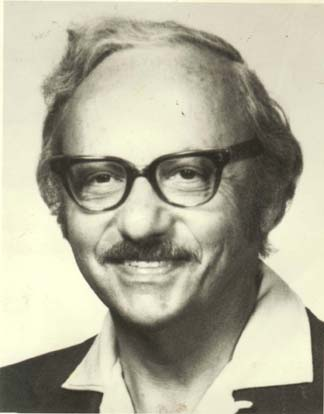
\includegraphics[scale=0.5]{figuren/lp/dantzig.jpg} 
     \caption{George B. Dantzig (1914--2005)}
    \label{fig:dantzig}
\end{figure}
In een interview uit 1986 vertelde Dantzig hoe hij zijn licentiaatsdiploma
in de wiskunde haalde zonder een thesis te schrijven. Blijkbaar
kwam hij eens te laat tijdens een les binnen. Op het bord stonden
twee problemen. Dantzig loste ze op en gaf ze een paar dagen later
af aan zijn professor. Hij verontschuldigde zich dat het zolang
geduurd had, maar deze huiswerkvragen vond hij toch iets moeilijker
dan gewoonlijk. Een paar weken later kreeg Dantzig zijn professor
op bezoek, die net zijn (correcte) oplossingen had bekeken. De
vragen aan het bord waren echter helemaal niet bedoeld als huiswerk,
maar het waren twee bekende onopgeloste problemen uit de statistiek!
De professor stelde tenslotte voor om deze twee antwoorden als
thesis te laten dienen.

Wat is nu juist een probleem uit de lineaire programmering? Een
poging tot \emph{definitie} is:

\begin{quote}
    Een lineair programmeringsprobleem bestaat erin een lineaire
doelfunctie van twee (of meer) onbekenden maximaal of minimaal
te maken. Deze onbekenden zijn onderworpen aan beperkingen die
(meestal)
de vorm aannemen van een stelsel lineaire ongelijkheden. Bijna
altijd eisen we dat onbekenden niet negatief mogen zijn.
\end{quote}

Volgend schema kan dienst doen als leidraad bij het oplossen
van oefeningen:

\begin{enumerate}
    \item  Vertaal het probleem naar wiskunde.
    \begin{itemize}
        \item  Maak indien mogelijk een overzicht van alle gegevens (bvb.\ in tabelvorm).

        \item  Bepaal wat de onbekende grootheden zijn. Geef ze
een naam.

        \item  Schrijf de beperkingen als lineaire ongelijkheden.

        \item  Zoek de doelfunctie (die minimaal of maximaal moet gemaakt
worden).
    \end{itemize}

    \item  Teken de \emph{geldige oplossingenverzameling}.
    \begin{itemize}
        \item  Schrijf de ongelijkheden in de standaardvorm (is
niet altijd nodig).

        \item  Teken de rechte die met elke ongelijkheid overeenkomt.

        \item  Bepaal het juiste halfvlak.
    \end{itemize}

    \item  Teken \'{e}\'{e}n van de \emph{doelfuncties} (geef een waarde
    aan $W$
of \emph{K}). Verschuif deze rechte evenwijdig tot ze net de geldige
oplossingenverzameling gaat verlaten. Bepaal  de co\"{o}rdinaten van het \emph{hoekpunt}.

    \item  Geef een \emph{volledig antwoord} op de vraag.
\end{enumerate}


%
%
%\newpage
%\section{De hoekpuntmethode}
%De methode die in beide voorbeelden hierboven werd gebruikt,
%is in essentie puur grafisch. In beide gevallen vonden we door
%de doelfunctie (isokosten- of isowinstrechte) te verschuiven,
%het optimale punt dat toch nog net tot de verzameling van alle
%geldige oplossingen behoorde.
%
%Het is niet toevallig dat die optimale oplossing telkens een
%\emph{hoekpunt} was van de verzameling geldige oplossingen. De `hoekpunt'-methode
%maakt hier dankbaar gebruik van. Ze steunt op volgende stelling
%(die we zonder bewijs geven).
%
%
%\subsection{Fundamentele stelling van de lineaire programmering}
%Als de geldige oplossingenverzameling begrensd is (een veelhoek,
%zoals in het maximalisatie-vraagstuk uit paragraaf~\ref{sec.maxprob}), dan heeft de doelfunctie zowel een maximum als
%een minimum. Beiden worden bereikt in \'{e}\'{e}n van de hoekpunten
%van de geldige oplossingenverzameling.
%
%Als deze verzameling niet begrensd is (zoals in het
%minimalisatievoorbeeld uit paragraaf~\ref{sec.minprob}),
%bestaat de mogelijkheid dat de doelfunctie geen minimum of geen
%maximum bereikt. Maar \emph{als} er wel een minimum of maximum bestaat,
%zal het met zekerheid voorkomen in een hoekpunt!
%
%
%
%\subsection{Voorbeeld 1 met de hoekpuntmethode}
%We hernemen in figuur~\ref{fig:hoekpuntmethode} even de
%tekening van de geldige oplossingenverzameling.
%\begin{figure}[htbp]
%    \centering
%\begin{tikzpicture}[scale=0.5]
%\draw[->] (-1,0) -- (17,0) node[right] {$x$};
%\draw[->] (0,-1) -- (0,17) node[above] {$y$};
%\foreach \x in {2,4,...,16}
%	\draw[shift={(\x,0)}] (0pt,2pt) -- (0pt,-2pt) node[below] {\footnotesize $\x$};
%\foreach \y in {2,4,...,16}
%	\draw[shift={(0,\y)},color=black] (2pt,0pt) -- (-2pt,0pt) node[left] {\footnotesize $\y$};
%\node [below left] at (0,0) {\footnotesize 0};	
%%	\fill[pattern=north east lines, pattern color=gray]  (-1,12.2) -- (5,11)-- (10,6) -- (10,-1) -- (18,-1) -- (18,17) -- (-1,17) -- cycle;
%\draw[dotted](-1,12.2) -- (14,9.2);
%\draw[dotted](10,-1) -- (10,12);
%\draw[dotted](-1,17) -- (17,-1);
%\draw[very thick, red] (0,0) -- (10,0) -- (10,6) -- (5,11) -- (0,12) -- cycle;
%\node (A) [above right, donkergroen] at (0,0) {A(0,0) $\Rightarrow W=0$};
%\filldraw [donkergroen] (0,0) circle (4pt);
%\node (B) [above right, donkergroen] at (10,0) {B(10,0) $\Rightarrow W=250$};
%\filldraw [donkergroen] (10,0) circle (4pt);
%\node (C) [above right, donkergroen] at (10,6) {C(10,6) $\Rightarrow W=700$};
%\filldraw [donkergroen] (10,6) circle (4pt);
%\node (D) [above right, donkergroen,draw,rounded corners,thick] at (5,11) {D(5,11) $\Rightarrow W=950$};
%\filldraw [donkergroen] (5,11) circle (4pt);
%\node (E) [above right, donkergroen] at (0,12) {E(0,12) $\Rightarrow W=900$};
%\filldraw [donkergroen] (0,12) circle (4pt);
%\end{tikzpicture}
%    \caption{Hoekpuntmethode}
%    \label{fig:hoekpuntmethode}
%\end{figure}
%
%Deze gesloten veelhoek heeft vijf hoekpunten. Het enige wat we nu
%moeten doen is elk hoekpunt invullen in de doelfunctie.
%Vermits de geldige oplossingenverzameling begrensd is, ben je
%zeker dat \'{e}\'{e}n van de hoekpunten de maximale, en \'{e}\'{e}n de
%minimale waarde van de doelfunctie zal opleveren.
%
%\begin{table}[hbp]
%    \centering
%    \caption{Winst in elk hoekpunt}
%    \begin{tabular}{cr}
%        \toprule
%        Hoekpunt & Winst  \\
%        \midrule
%        A(0,0) & 0  \\
%        B(0,12) & 900  \\
%        C(5,11) &   950\\
%        D(10,6) &700 \\
%        E(10,0) & 250  \\
%        \bottomrule
%    \end{tabular}
%    \label{tbl:hoeken}
%\end{table}
%
%Antwoord: De \emph{minimale} winst bereikt de boer als hij geen dieren
%houdt (\euros 0). De \emph{maximale} opbrengst krijgt hij
%door vijf kippen en elf schapen te houden (\euros 950).


\newpage
\section{Uitzonderlijke situaties}
Volgende puntjes komen bij echte praktische vraagstukken zelden
voor. Als ze dan toch de kop opsteken, wijst dit dikwijls op \emph{een
foutieve formulering van het lineair programmeringsprobleem}.
Voor een computerprogramma moeten deze uitzonderlijke situaties
toch bekeken worden.



\subsection{G\'{e}\'{e}n punten in de geldige oplossingenverzameling}
Bekijk volgend lineair programmeringsvraagstuk:
Maximaliseer
\begin{displaymath}
    P=x+2y
\end{displaymath}
Met als beperkingen
\begin{eqnarray*}
    x+y & \geqslant & 3  \\
    x+2y & \leqslant & 2  \\
    2x+y & \leqslant & 2  \\
    x \mbox{ en } y & \geqslant & 0
\end{eqnarray*}
Maak zelf een tekening voor deze opgave. Als we dit systeem van vijf ongelijkheden proberen op te lossen,
moeten we alle punten zoeken die niet in gearceerd gebied liggen. Je
merkt op de tekening dat er geen enkel dergelijk punt bestaat.



\subsection{Meer dan \'{e}\'{e}n optimaal punt}
Als de doelfunctie evenwijdig loopt met \'{e}\'{e}n van de grenslijnen
van de geldige oplossingenverzameling, is elk punt op deze grenslijn
een optimaal punt. Bekijk even volgende opgave:
Maximaliseer
\begin{displaymath}
    P=2x+y
\end{displaymath}
Met als beperkingen
\begin{eqnarray*}
    2x+y & \leqslant & 2  \\
    x+2y & \leqslant & 2  \\
    x \mbox{ en }y & \geqslant & 0
\end{eqnarray*}
Maak opnieuw zelf de tekening.



\subsection{Onbegrensde oplossingenverzameling bij maximalisatie}
Maximaliseer:
\begin{displaymath}
    P=x+y
\end{displaymath}
Met als beperkingen
\begin{eqnarray*}
    -x+y & \leqslant & 1  \\
    y & \leqslant & 2  \\
    x \mbox{ en } y & \geqslant & 0
\end{eqnarray*}
Maak de figuur en laat zien dat je $P$ zo groot kan maken als je maar wil.


\newpage
\section{Meerdere onbekenden}
In dit hoofdstukje beperkten we ons tot problemen met twee onbekenden
(bvb.\ het aantal kippen en het aantal schapen).

Er bestaan echter ook methodes om lineaire programmeringsvraagstukken
met meerdere onbekenden op te lossen (bvb.\ de simplexmethode).
Dit komt in het tweede semester aan bod in het OPO Toegepaste Wiskunde 2.

%\end{document}

\newpage 
%%%%%%%%%%%%%%%%%%%%%%%%%%%%%%%%%
% Laatste aanpassing: 
% 5/1/14 [Jan]: oplossing oefening loften aangepast (suggestie Inge)
%
% 26/06/13 [Greetje]: Oefeningen van Leentje toegevoegd
% 18/2/12 [Jan]: Oef 7 aangepast
%
% 2/2/11 [Greetje]: nieuwe oefeningen toegevoegd. Formulering van sommige oefeningen aangepast.
%
% 14/09/10 [Greetje]: opgaven in 3 veranderlijken verwijderd. Herhalingsvragen weggelaten.
%
% 11/9/07 [Jan]: enkele fouten verbeterd
%          
% 14/9/05 [Jan]: vraag is 10 stoelen (i.p.v. 30)
%
% 8/09/01 door Greetje
%   correcties van Roos en Roby
%
% nieuwe aanpassing: 8/06/02 door Roos  %
%  nieuwe opgaven en volgorde veranderd       %
%%%%%%%%%%%%%%%%%%%%%%%%%%%%%%%%%

%\chapter{Oefeningen op lineaire programmering}
\section{Oefeningen}
\begin{oef}
De Indische regering kondigt een ambitieus plan aan om in
     ieders voedselbehoefte te kunnen voorzien op basis van rijst en
     sojascheuten. E\'{e}n kopje ongekookte rijst kost \euros{0,20} en bevat
     15 gr eiwitten, 810 calorie\"{e}n en $\frac{1}{9}$ mg vitaminen
     B2. E\'{e}n kopje sojascheuten kost \euros{0,40} en
     levert 22,5 gr eiwitten, 270 calorie\"{e}n en $\frac{1}{3}$ mg
     B2. Veronderstel dat de minimale dagelijkse
     behoeften er als volgt uitzien: 90 gr eiwitten, 1620 calorie\"{e}n
     en 1 mg vitamine B2.
 Hoe ziet het goedkoopste
     dieet dat voldoet aan de minimale behoeften eruit?
     \begin{opl}
     De goedkoopste oplossing (figuur~\ref{fig:oplrijstsoja}) die aan alle beperkingen voldoet is drie kopjes rijst en twee kopjes sojascheuten, met een kostprijs van \euros{1,40}. 
     \begin{figure}[hbtp]
\centering
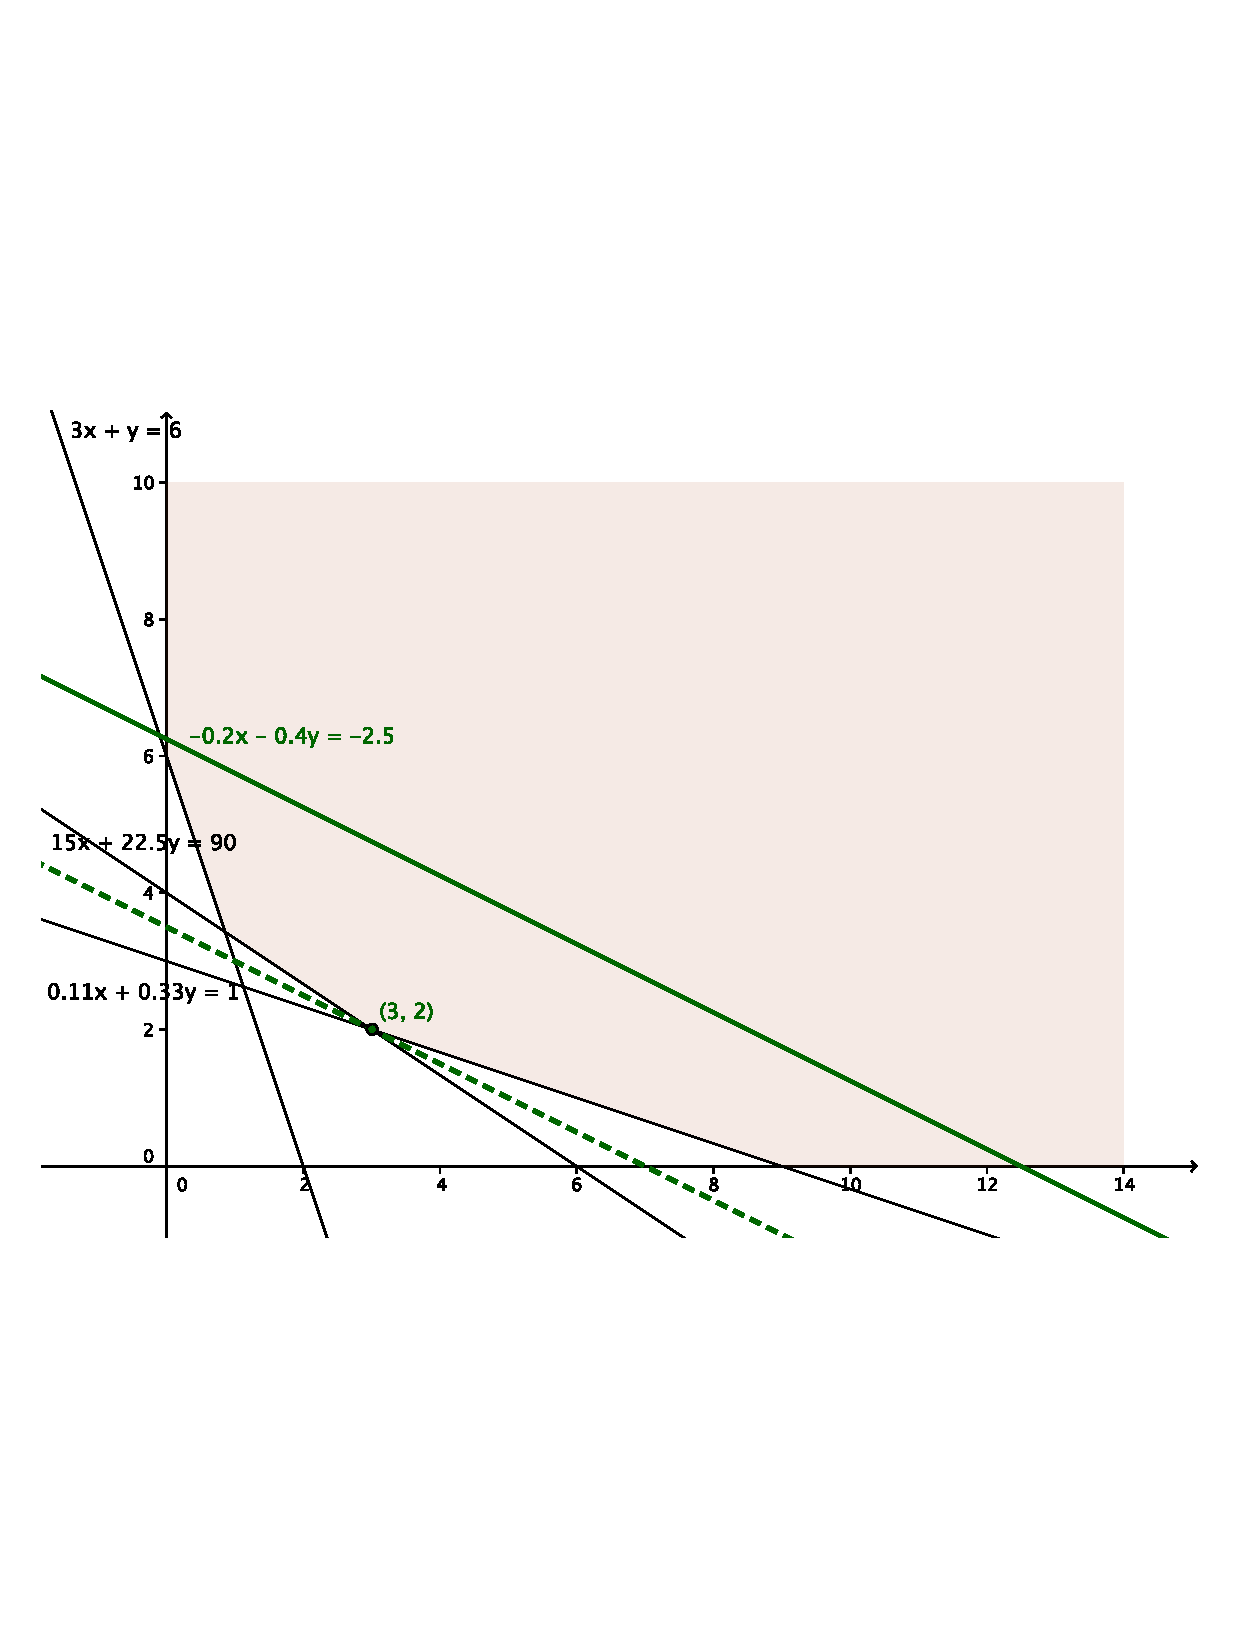
\includegraphics[width=0.8\textwidth]{oefeningen/FigurenLP/OefRijstSoja.pdf}
\caption{Optimaal punt is drie kopjes rijst en twee kopjes soja}
\label{fig:oplrijstsoja}
\end{figure}

     \end{opl}
\end{oef}
 
\begin{oef}
In een bedrijf worden nieuwe archiefkasten aangekocht. Er
     is keuze tussen 2 types met verschillende afmetingen en
     functies. Type A kost \euros{150} en is \SI{60}{\cm} diep, \SI{40}{\cm} breed en
     \SI{1}{\m} hoog. Type B kast kost het dubbele van A maar is \SI{45}{\cm}
     diep, \SI{80}{\centi\meter} breed en \SI{1,5}{\meter} hoog. Voor elke type A kast moeten
     minstens 2 kasten van type B geplaatst worden. De totale
     grondoppervlakte die in het bedrijf moet ingenomen worden door
     archiefkasten is minstens \SI{3,84}{\square\meter}. Er is in totaal \euros{7500}
     voorzien voor de aankoop. Hoeveel kasten van elk type moeten
     er aangekocht worden om de kostprijs zo laag mogelijk te houden? 
     \begin{opl}
     Vier kasten van type A en acht kasten van type  B leveren de goedkoopste prijs van \euros{3000} en voldoen aan alle voorwaarden (figuur~\ref{fig:kastenAB}).
          \begin{figure}[hbtp]
\centering
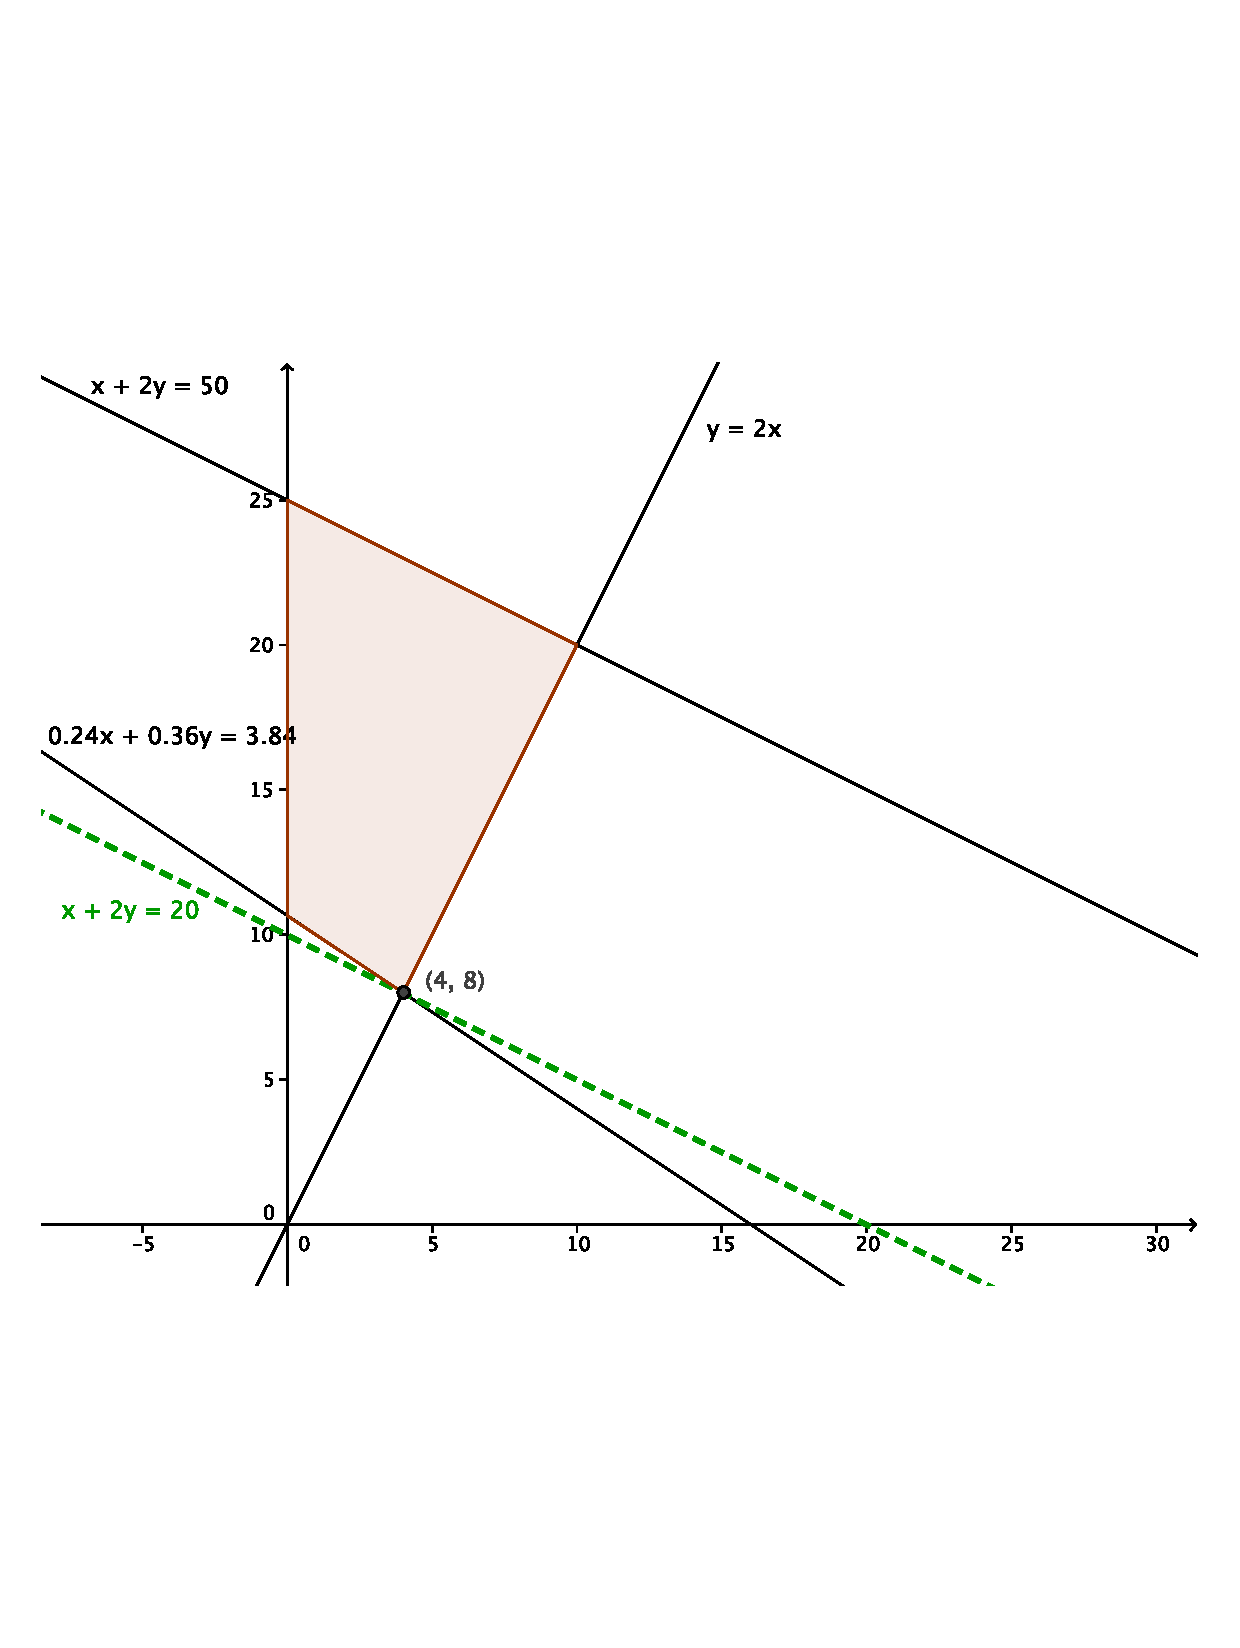
\includegraphics[width=0.8\textwidth]{oefeningen/FigurenLP/OefkastenAB.pdf}
\caption{Optimaal punt is vier kasten A en acht kasten B}
\label{fig:kastenAB}
\end{figure}
     \end{opl}
\end{oef}
     
     
   
\begin{oef}
Het departement G\&T wordt verkozen tot `Departement van het
    jaar'. Als beloning mogen alle personeelsleden en studenten -- in
    totaal 2000 mensen -- gratis voor  \'{e}\'{e}n week op reis naar
    Kreta. `Cobol Airlines' zorgt voor het transport. 
\begin{figure}[h]
\centering
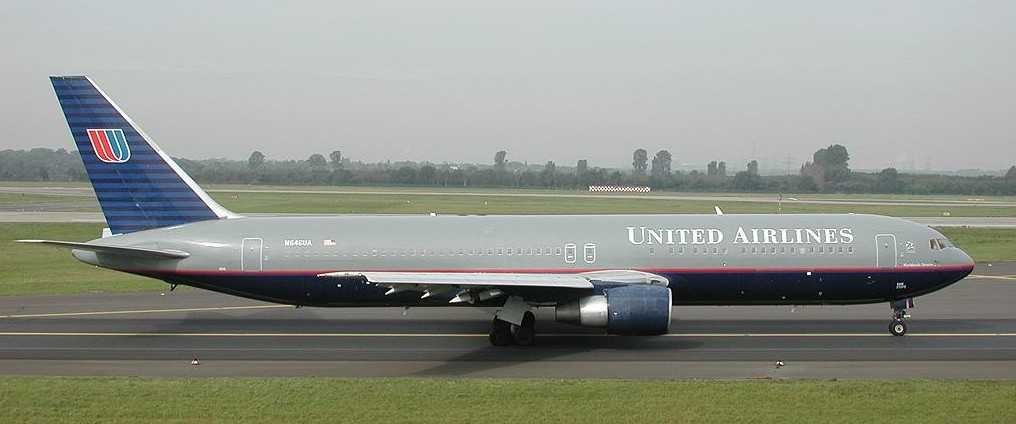
\includegraphics[width=0.8\textwidth]{oefeningen/FigurenLP/Boeing-767.jpg}
\caption{Boeing 767-300}
\end{figure}
    Deze
    luchtvaartmaatschappij beschikt over een vloot van Fokkers en
    Boeings 767. De Fokker heeft een capaciteit van 80 passagiers,
    heeft 3 stewards aan boord en kost per vlucht \euros{20\,000}. De
    Boeing 767 kan 240 personen meenemen, vraagt 4 Stewards en kost
    \euros{100\,000} per vlucht.`Cobol Airlines' beschikt over 50
    stewards. Er moeten minstens evenveel Fokkers als Boeings
    ingezet worden voor het vervoer van deze 2000 mensen.
Wat is de samenstelling van toestellen zodat 
	de reis zo goedkoop mogelijk
    wordt? Hoeveel kost de reis?   
    \begin{opl}
    Tien Fokkers en vijf Boeings leveren de goedkoopste transportoplossing (figuur~\ref{fig:deptjaar}) met een kostprijs van \euros{700\,000}.
              \begin{figure}[hbtp]
\centering
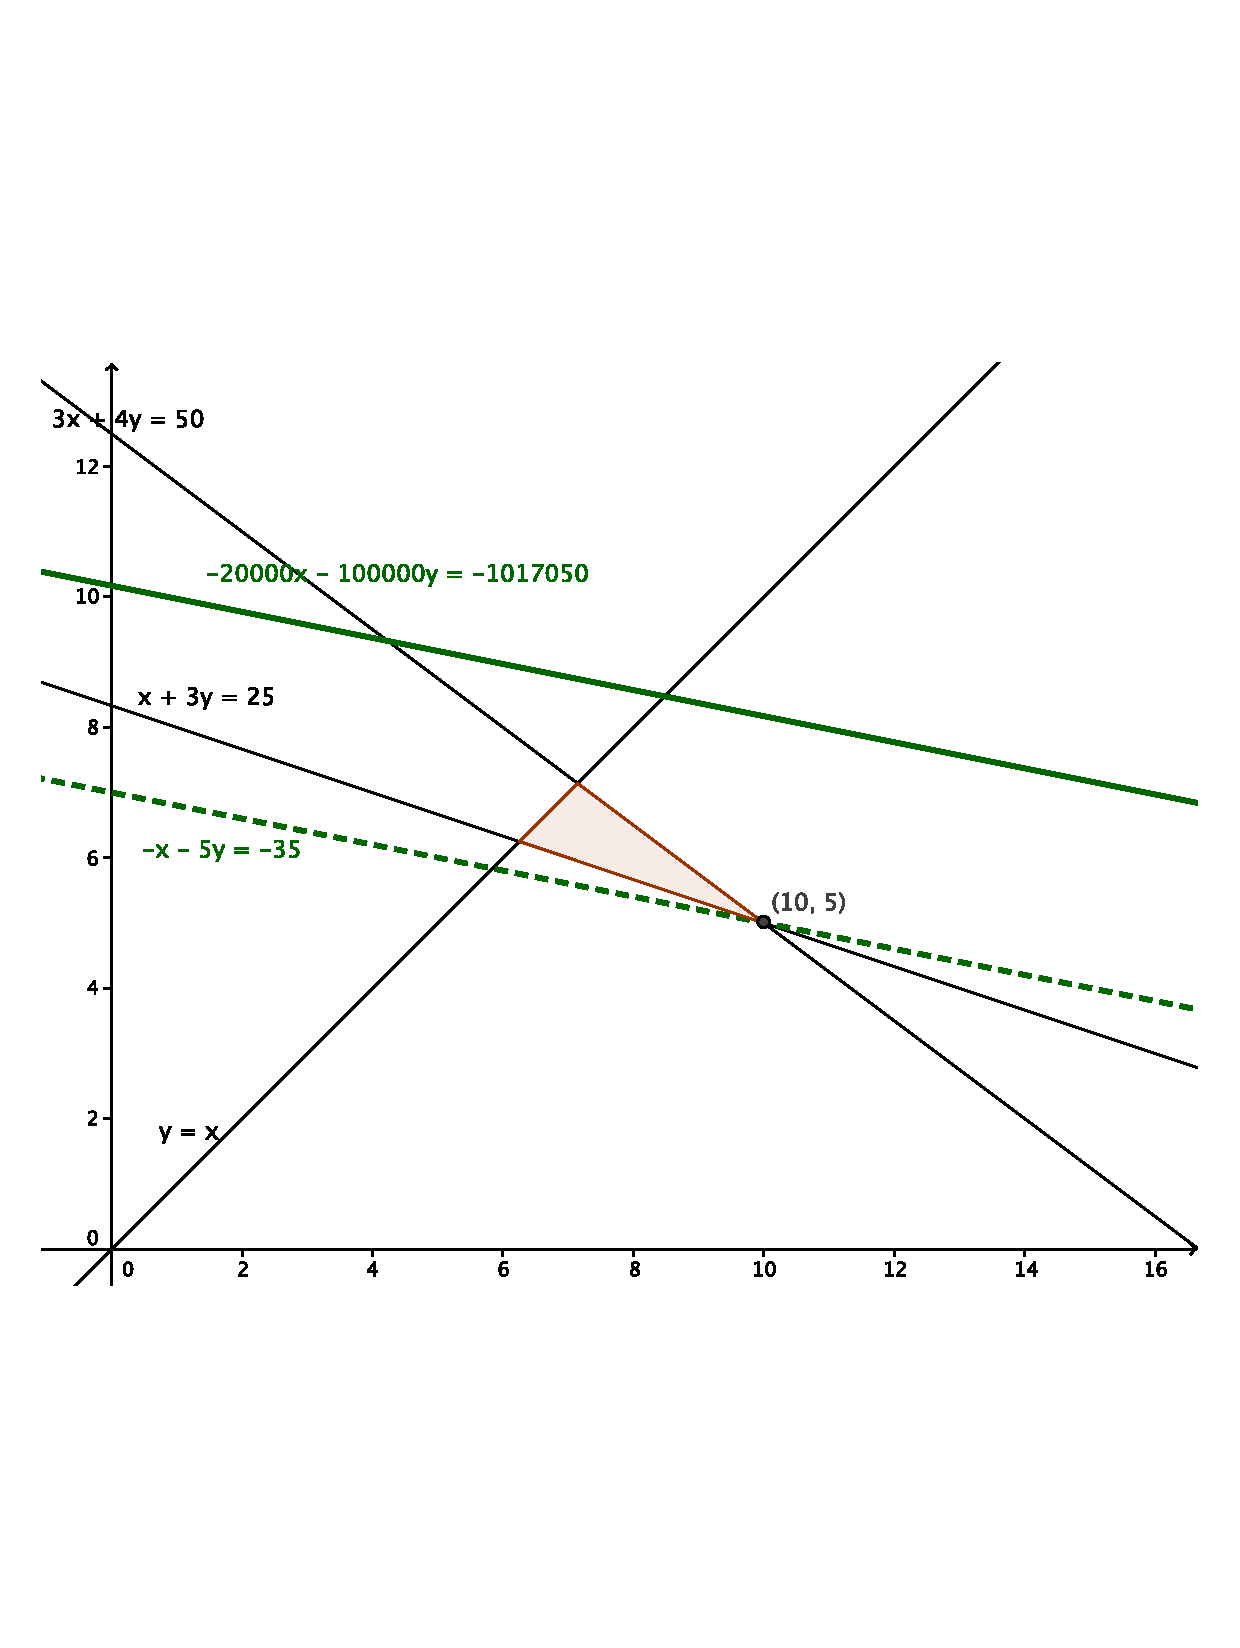
\includegraphics[width=0.8\textwidth]{oefeningen/FigurenLP/OefDepvhjaar.pdf}
\caption{Optimaal punt is 10 Fokkers en 5 Boeings}
\label{fig:deptjaar}
\end{figure}
    \clearpage
    \end{opl}
\end{oef}      

\begin{oef}
Artsen zonder Grenzen plannen een konvooi om de
     noodlijdende bevolking van een vluchtelingenkamp in Afghanistan te 
     bevoorraden met tenten en dekens, zodat de mensen de winter kunnen 
     doorkomen. Per tent worden minstens drie dekens geleverd. Het totale laadvermogen van alle voertuigen samen is 
     10 ton. Een tent weegt 2 kg en een deken 1 kg. Er zijn slechts 8000 dekens beschikbaar. Met een tent kan men 
     5 vluchtelingen helpen, met een deken slechts \'{e}\'{e}n 
     vluchteling. Hoeveel tenten en dekens moet men leveren om zoveel 
     mogelijk mensen te helpen? 
     \begin{opl}
     Met 2000 tenten en 6000 dekens kunnen in totaal 16\,000 mensen geholpen worden (figuur~\ref{fig:AZG}).
                   \begin{figure}[hbtp]
\centering
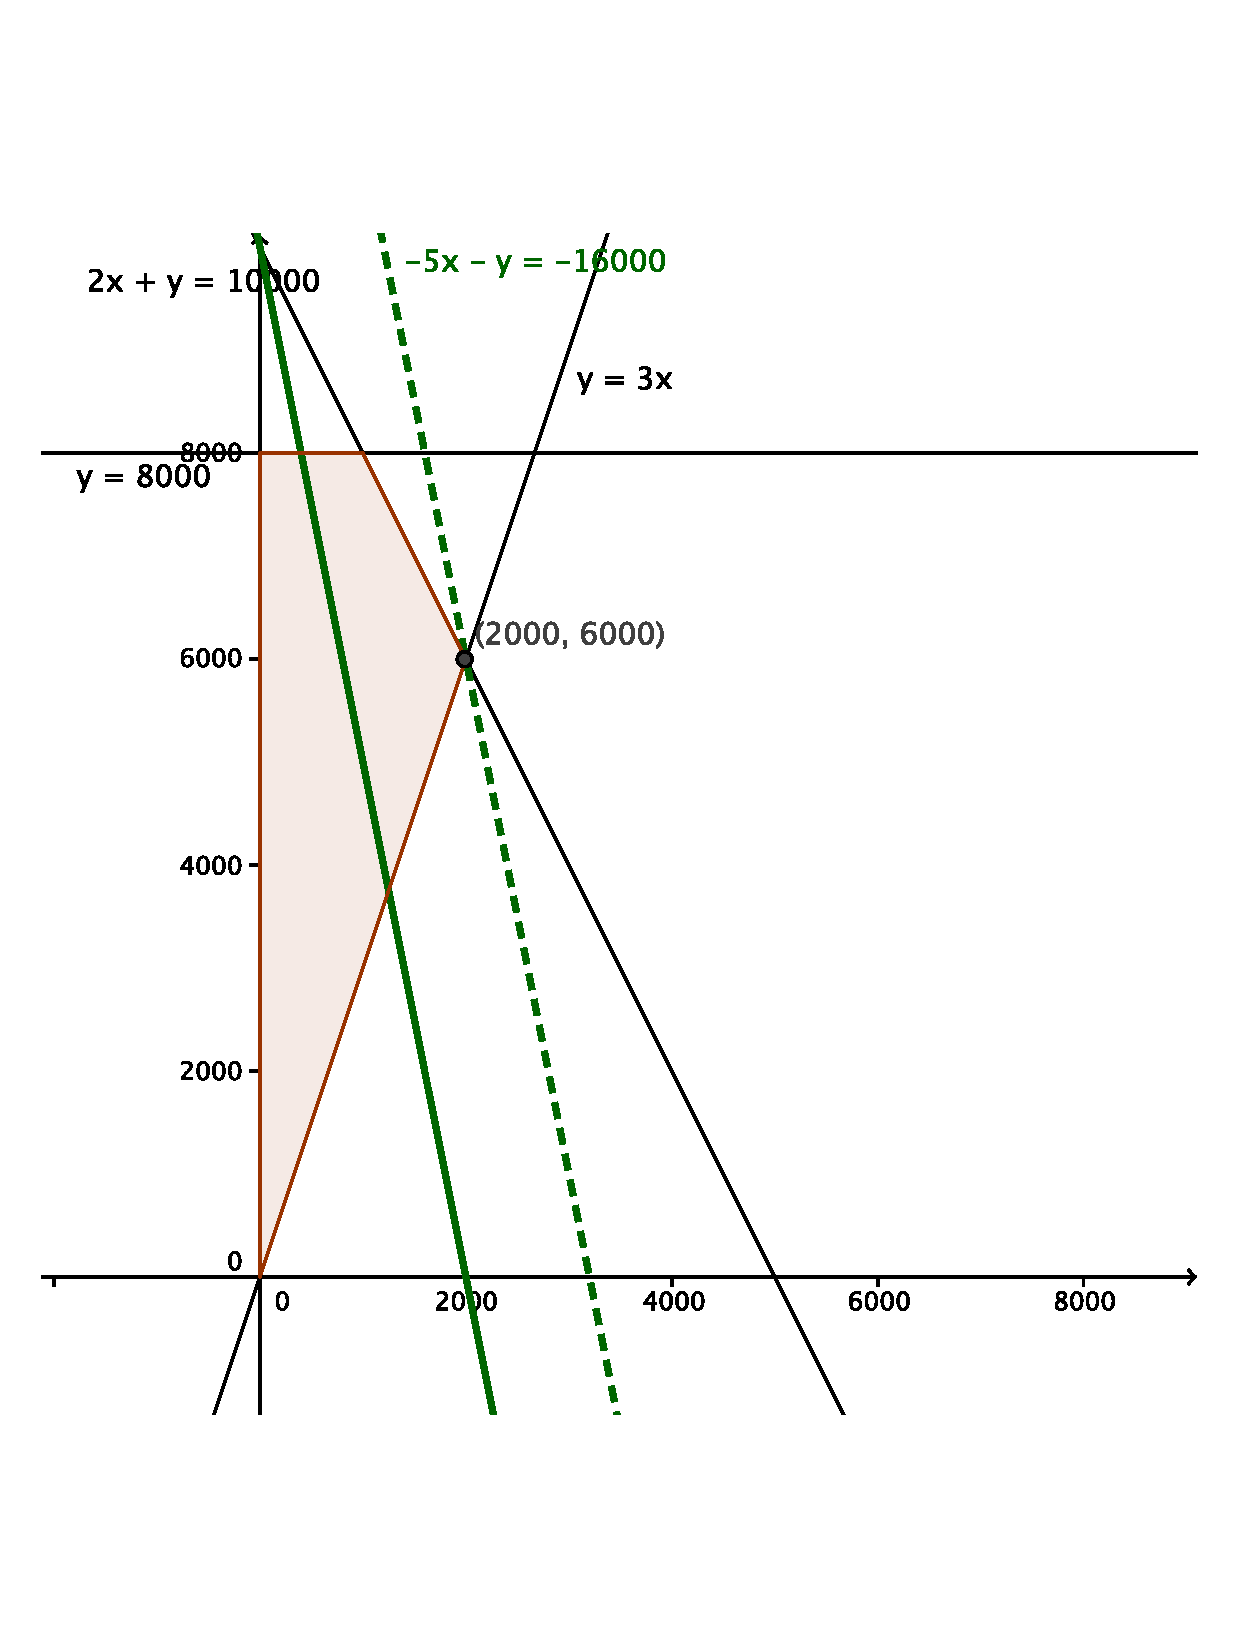
\includegraphics[width=0.7\textwidth]{oefeningen/FigurenLP/OefAZG.pdf}
\caption{Optimaal punt is 2000 tenten en 6000 dekens}
\label{fig:AZG}
\end{figure}
     \end{opl}
\end{oef}
     
\begin{oef}
In een speelgoedfabriek worden Woody
en Buzz Lightyear poppen gemaakt. 
\begin{figure}[ht]
  \centering
    
\includegraphics[scale=0.5]{oefeningen/FigurenLP/Buzz-Woody.jpg}
\end{figure}
Omwille van beperkingen van machines
kunnen er dagelijks in totaal maximaal 100 poppen gemaakt worden. De
directie van de fabriek heeft besloten om minstens 10 Buzz Lightyear
poppen en hoogstens 80 Woody poppen te maken per dag. 
De milieubijdrage
voor een Buzz Lightyear pop is 2 euro terwijl die maar de helft
bedraagt voor een Woody pop. De directie wil dagelijks niet meer dan 130
euro voorzien als milieubijdrage. Wegens de grotere populariteit van
Woody, worden er minstens evenveel Woody poppen gemaakt als Buzz
Lightyear poppen. Het bedrijf maakt een winst van 20 euro per Woody pop
en 10 euro per Buzz Lightyear pop. \begin{enumerate}
	\item Bepaal de optimale dagelijkse productie van Woody en Buzz
Lightyear poppen zodat het bedrijf een maximale winst heeft.
(\textit{Je mag hierbij van uitgaan dat alle geproduceerde poppen ook
effectief zullen worden verkocht en dus winst opleveren.}) Vermeld
duidelijk en gedetailleerd welke stappen je hebt gevolgd om tot je
oplossing te komen.
	\item  Bereken de bijhorende maximale winst.
\end{enumerate}
\end{oef}
  
\begin{oef}
Een boer wil hoogstens 40 ha van zijn land bebouwen met
     ma\"{i}s en aardappelen. Uit ervaring weet hij dat per ha ma\"{i}s
     $3$ dagen
     (hand)werk mag gerekend worden en per ha aardappelen 10 dagen.
     Volgens zijn werkschema kan hij hoogstens 240 werkdagen besteden
     aan het met de hand bewerken van ma\"{i}s en aardappelen. De machines
     bezit hij samen met andere boeren zodat hij slechts gedurende 47
     extra dagen over de nodige machines kan beschikken. Voor de 
     ma\"{i}s kan men per dag  \'{e}\'{e}n ha bewerken met 
     machines en voor 
     de aardappelen bewerkt men per dag $\frac{2}{3}$ van een ha. 
     Uiteindelijk  moet het aandeel van de ma\"{i}s minstens  \'{e}\'{e}n
     derde van de totale bewerkte oppervlakte zijn. De opbrengst
     per ha
     voor ma\"{i}s \euros{1000} is en die van aardappelen \euros{3000}.
Bepaal de verdeling van bewerkte oppervlakte ma\"{i}s en
     aardappelen die een maximale opbrengst levert. Bereken ook die
     opbrengst. 
     \begin{opl}
     20 ha ma\"is, 18 ha aardappelen
     \end{opl}
\end{oef}
     
     
     
     
\begin{oef}
In een bedrijf produceert men tafels en stoelen. Voor de
     productie van \'{e}\'{e}n tafel is 3 maal zoveel hout nodig als
     voor de productie van \'e\'en stoel. Er is in het bedrijf voldoende
     hout aanwezig om per week 45 stoelen te maken. Een stoel vraagt echter
     heel wat afwerking, zodat er voor het maken van \'{e}\'{e}n
     stoel 2 maal zoveel personeel nodig is als voor een tafel. Het
     bedrijf beschikt over net voldoende personeel om 20 stoelen af te
     werken per week. De vraag naar tafels en stoelen samen, per week,
     is 10 stuks, zodat het bedrijf per week minstens 10 meubelstukken zal produceren. De winst per tafel is \euros{125} en die per stoel is
     \euros{75}. Hoeveel tafels en stoelen moet men produceren om de
        winst zo groot mogelijk te maken? Hoeveel bedraagt de winst?
        \begin{opl}
        10 tafels en 15 stoelen (figuur~\ref{fig:tafelstoelen}) leveren de grootste winst, nl \euros{2375}.
        \begin{figure}[hbtp]
\centering
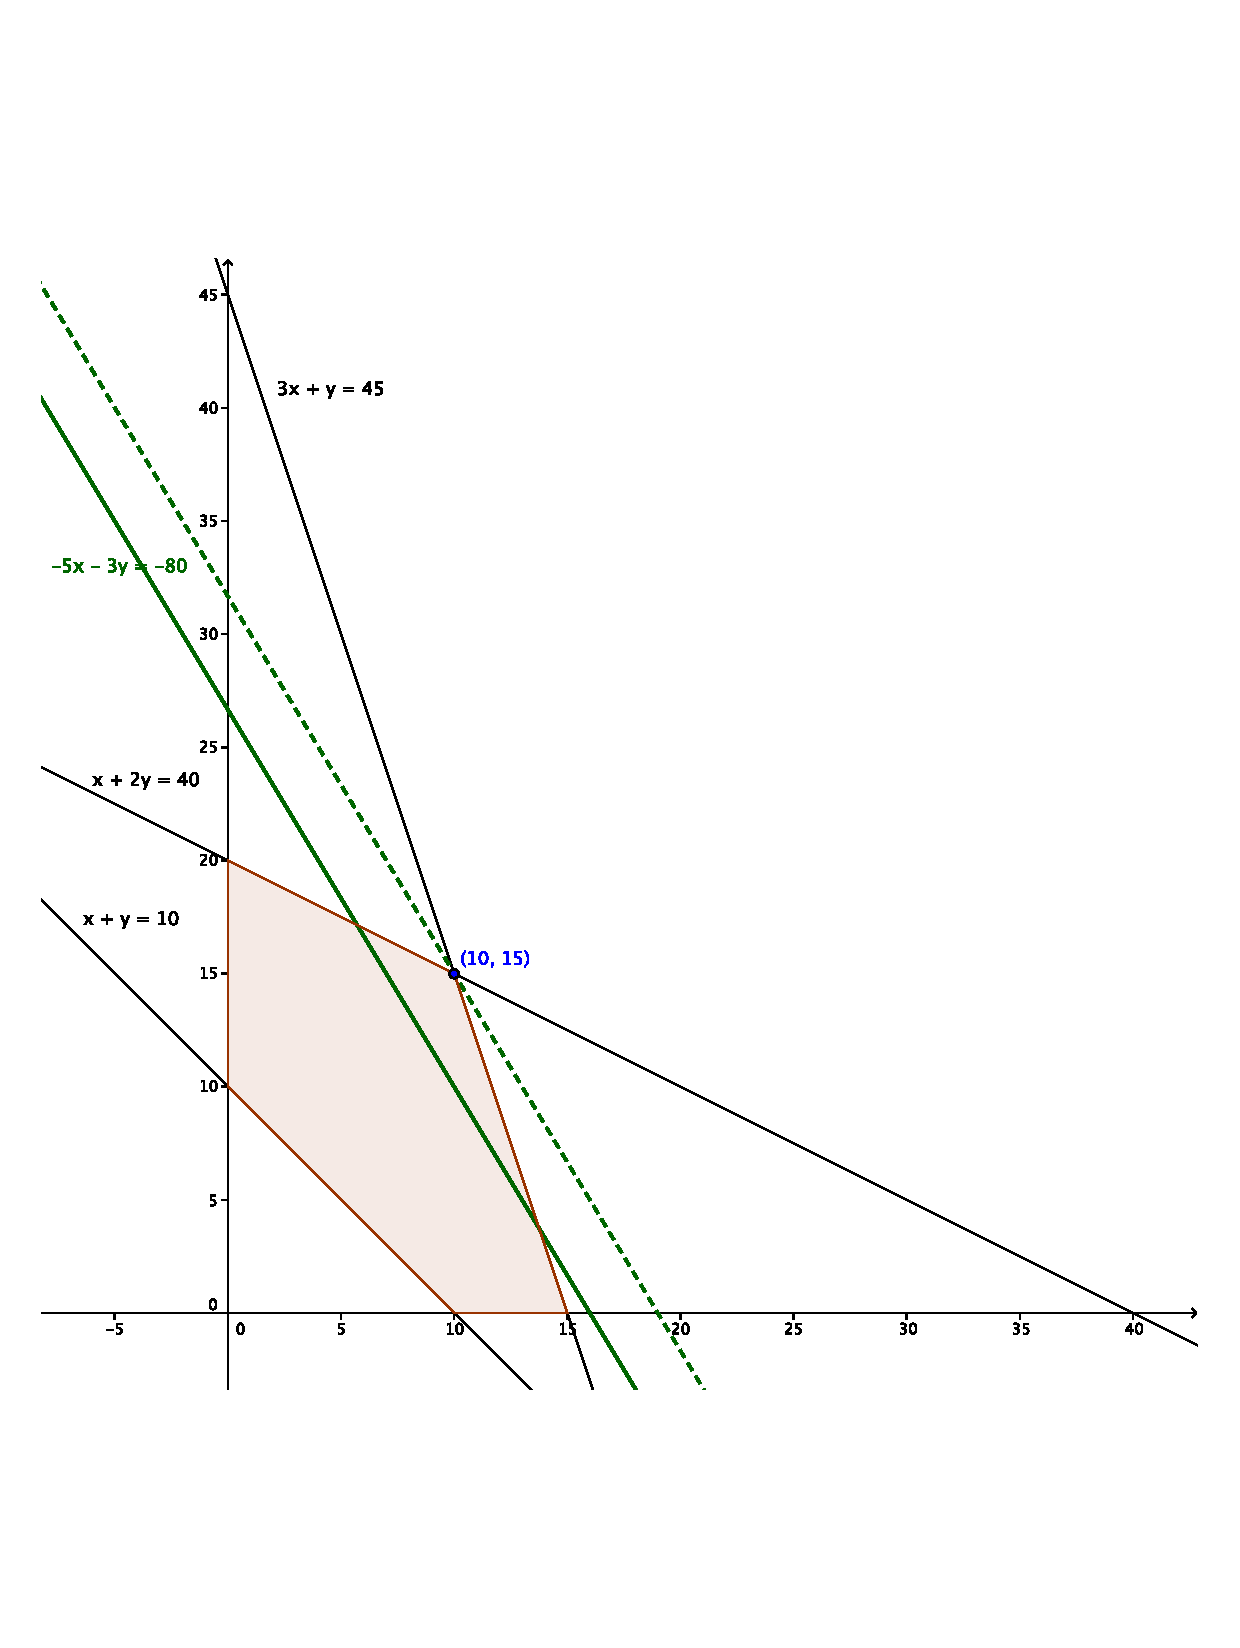
\includegraphics[width=0.8\textwidth]{oefeningen/FigurenLP/Oef7.pdf}
\caption{10 tafels en 15 stoelen leveren de grootste winst}
\label{fig:tafelstoelen}
\end{figure}
\clearpage
        \end{opl}
\end{oef}

     
\begin{oef}
Een bedrijf produceert 2 types containers.
     Voor de productie van 
    \'{e}\'{e}n container van type A is driemaal zoveel personeel 
    nodig als voor \'{e}\'{e}n container van type B. Het bedrijf 
    beschikt over voldoende personeel om 120 containers van type B te 
    maken per dag. Voorts vereist \'{e}\'{e}n container van type B 
    tweemaal zoveel staal als \'{e}\'{e}n container van type A. Er is 
    in het bedrijf voldoende staal aanwezig om per dag 60 containers 
    van type A te maken. De winst per container van type A is \euros {2500} 
    en die per container van type B is \euros{1000}. Er is elke dag 
    vraag naar \emph{minstens} 15 containers van beide types samen. Het 
    aandeel van containers van type A is minstens \'{e}\'{e}n  vierde 
    van de dagelijkse productie van beide types containers \emph{samen}. 
    \emph{Hoeveel} containers van type A en hoeveel van type B moet 
    het bedrijf produceren om de winst zo groot mogelijk te maken?
    \begin{opl}
    De maximale winst (\euros{102\,000}) wordt bereikt bij de productie van 36 containers van type A en 12 containers van type B (figuur~\ref{fig:containersAB}).
            \begin{figure}[hbtp]
\centering
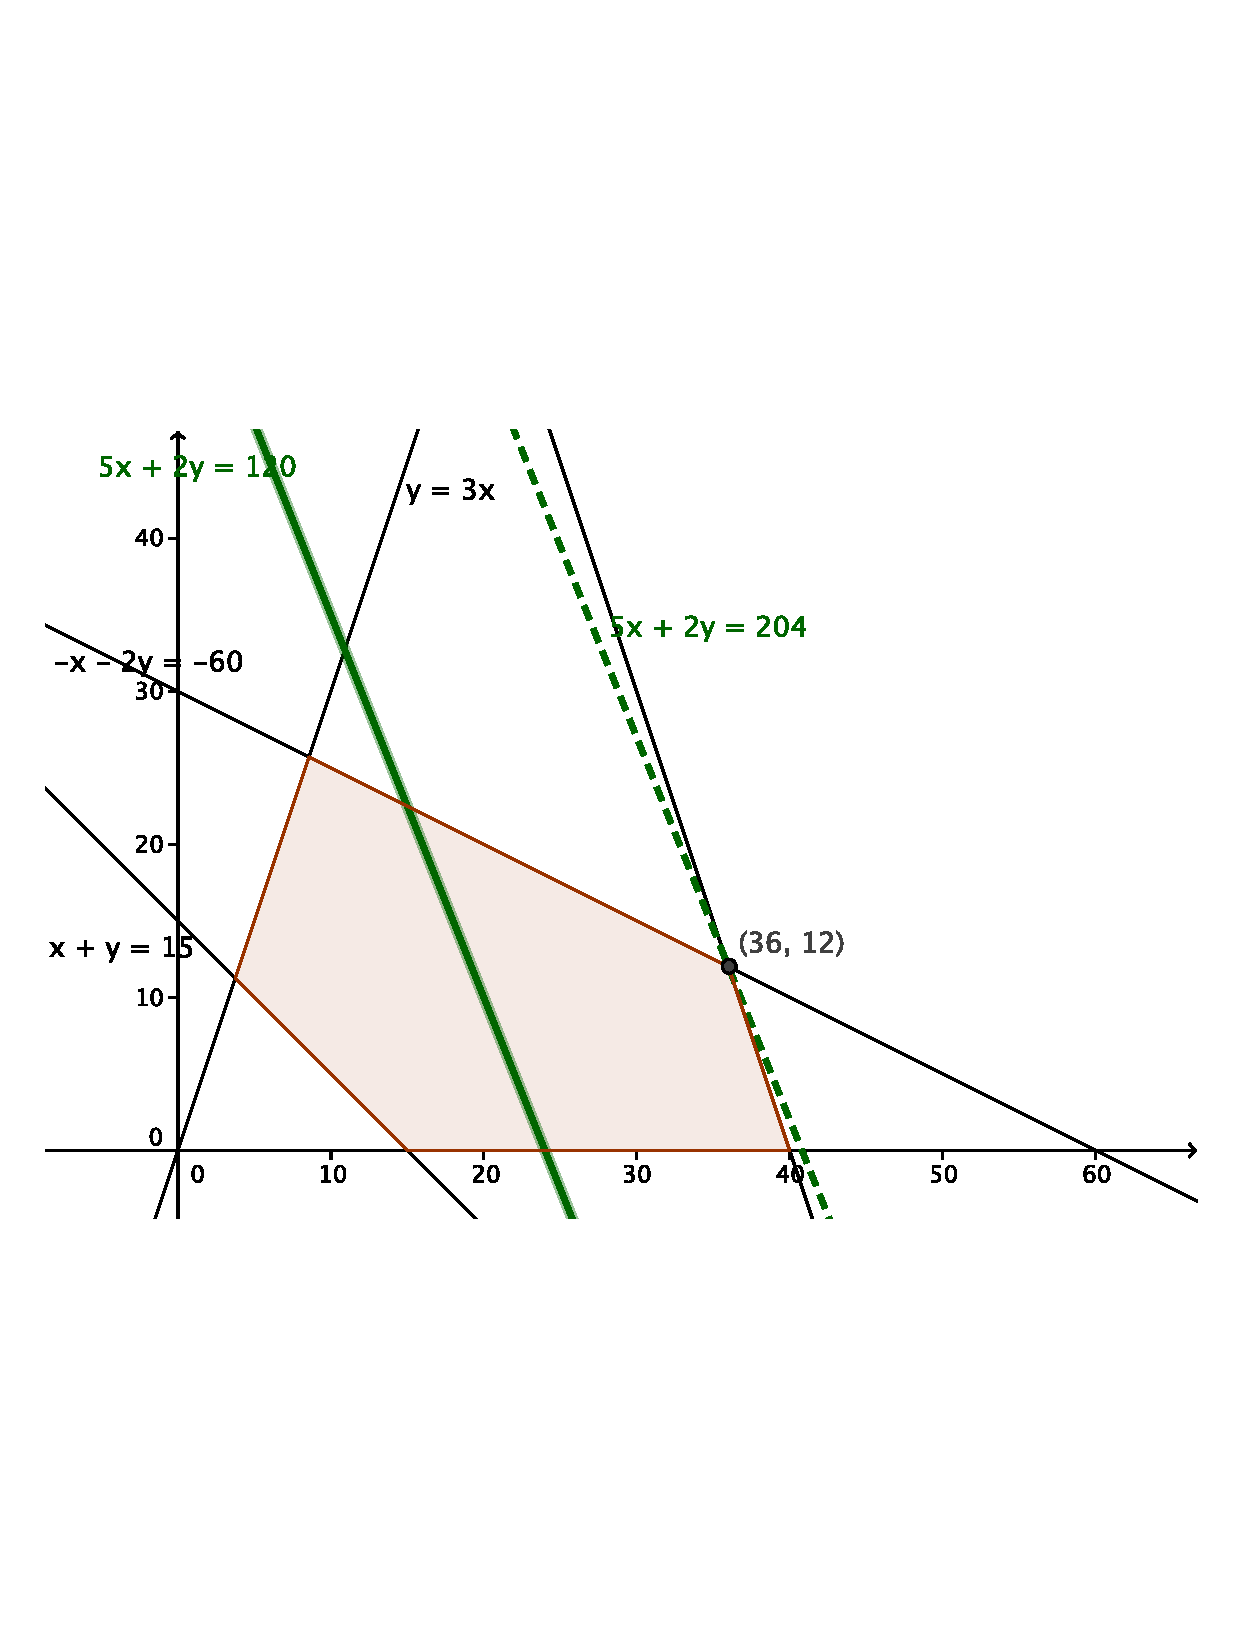
\includegraphics[width=0.8\textwidth]{oefeningen/FigurenLP/OefcontainersAB.pdf}
\caption{De grootste winst is bij 36 containers A en 12 containers B}
\label{fig:containersAB}
\end{figure}
    \end{opl}
\end{oef}

\begin{oef}
Een fabriek produceert metalen platen en buizen.
     Het aantal machines voor deze productie laat toe om maximaal 35
     ton platen \emph{of} 70 ton buizen per maand te maken. Hiervoor zijn 80
     arbeiders beschikaar. E\'en man kan per maand 1 ton platen \emph{of} 500
     kg buizen verwerken. De buizen vereisen een nabehandeling in een
     andere afdeling waar slechts 35 ton per maand kan afgewerkt
     worden.   De opbrengst voor de fabriek op \'e\'en ton platen en
     \'e\'en ton buizen is respectievelijk \euros{2500} en
     \euros{2000}. Bepaal  de optimale
     productie waardoor de fabriek een maximale opbrengst bekomt. 
     \begin{opl}
     Een maandproductie van 20 ton platen en 30 ton buizen (figuur~\ref{fig:platenbuizen}) levert de maximale winst van \euros{110\,000}.
                 \begin{figure}[hbtp]
\centering
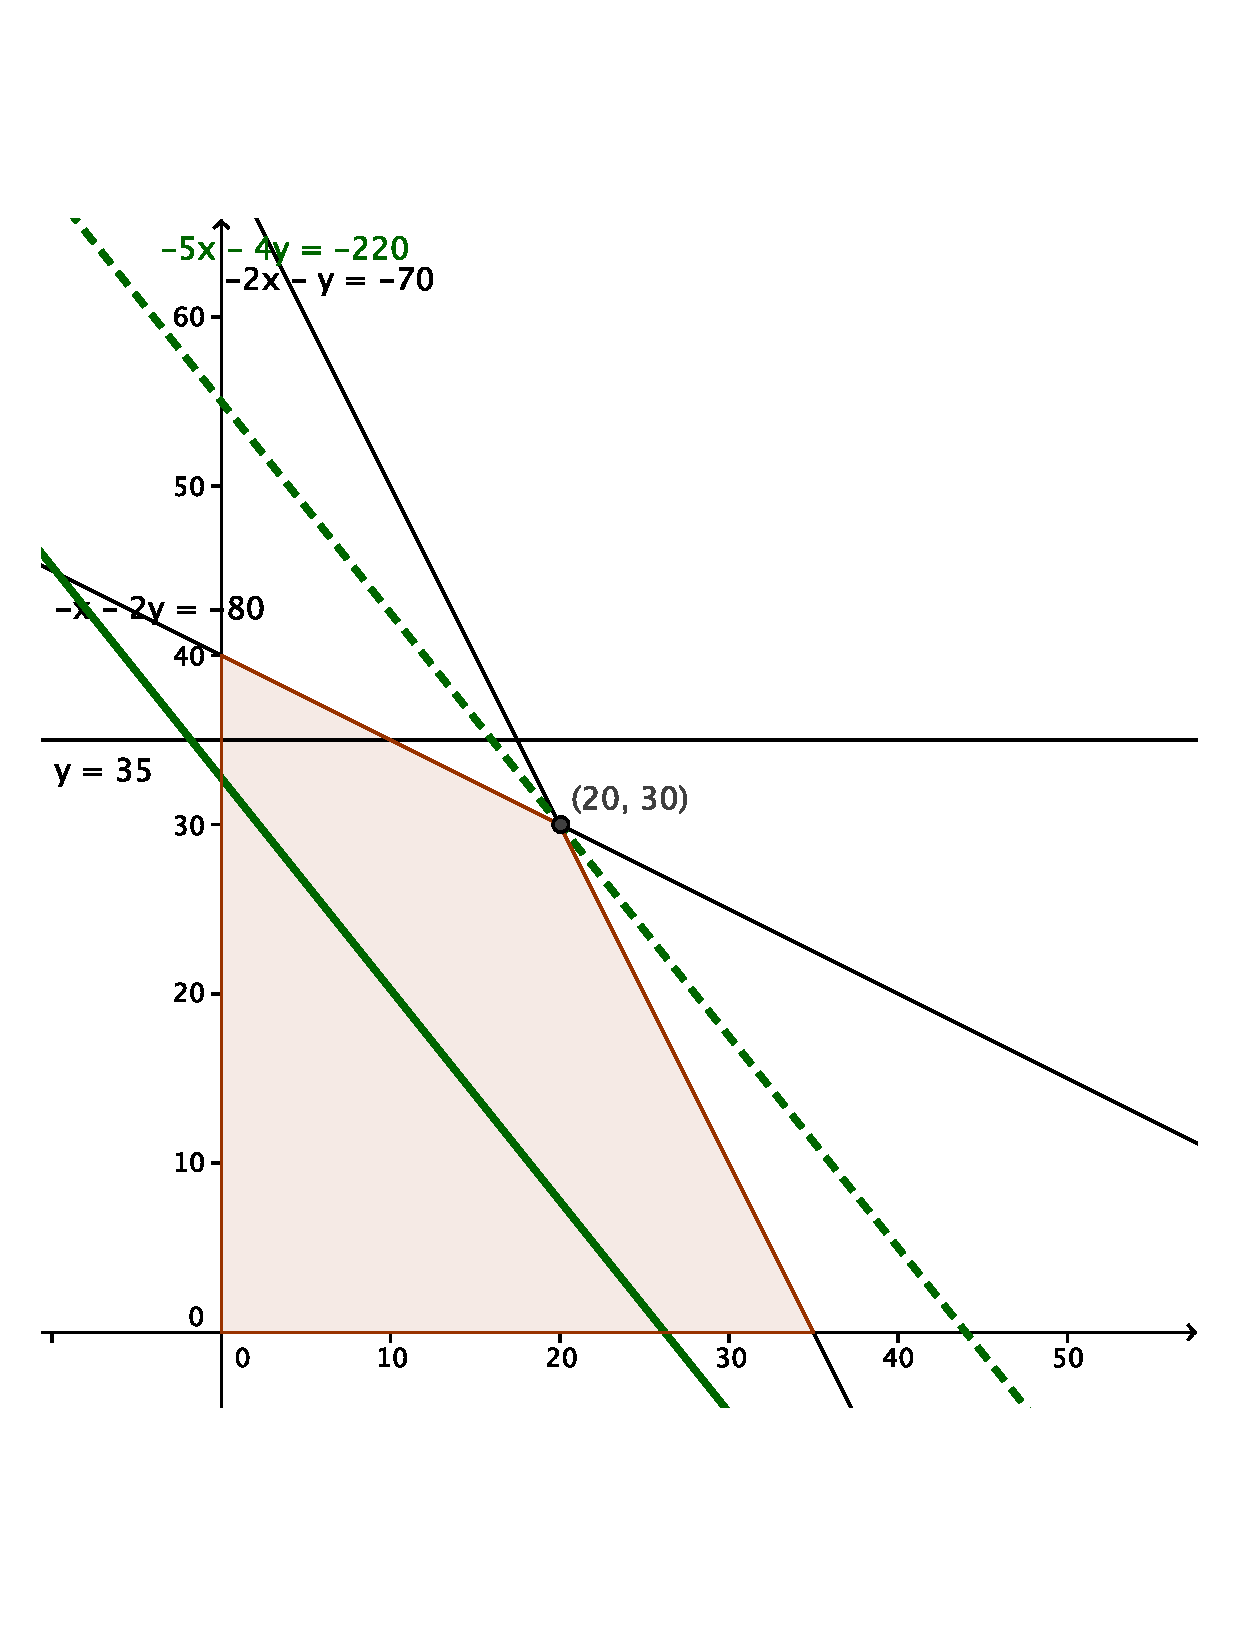
\includegraphics[width=0.8\textwidth]{oefeningen/FigurenLP/OefPlatenBuizen.pdf}
\caption{Maximale winst bij 20 ton platen en 30 ton buizen}
\label{fig:platenbuizen}
\end{figure}
\clearpage
     \end{opl}
\end{oef}
     


\begin{oef}
Een bioscoopzaal draait voorlopig alleen 
    `The lord of de Rings (LR) en `Harry Potter en de steen der wijzen' (HP). Bij 
     voorstellingen van LR laat men maximaal 100 volwassenen en 50 
     kinderen toe (inkomprijs \euros{8} resp.\ \euros{6}). Bij HP is dat 
     40 volwassenen en 160 kinderen (inkomprijs \euros{7} resp.\ 
     \euros{4}).  De onkosten 
     (personeel, rechten, apparatuur\ldots) voor 
     een voorstelling van LR bedragen \euros{200} voor HP \euros{120}.  De 
     totale winst van alle voorstellingen samen moeten minstens 
     \euros{21600} bedragen. Het poetswerk na een vertoning van LR duurt 
     10 minuten en bij HP 20 minuten. Het poetspersoneel mag in totaal  
     maximum 7.5 uren werken. De filmdistributeur bepaalt dat het aantal 
     vertoningen van LR  maximum 30 bedraagt en minstens 
     evenveel als het aantal vertoningen van HP. We veronderstellen 
          dat alle vertoningen vol geboekt zijn.
     Hoeveel voorstellingen van elke film moet men geven opdat het aantal 
     kinderen dat naar de film kan zo groot mogelijk is? 
     \begin{opl}
     15 voorstellingen van elke film
     \end{opl}
\end{oef}
     

\begin{oef}
De directie van een pretpark buigt zich over de uitbreiding van het
parkeerterrein met een aanpalend stuk grond. Op de parking kunnen zowel auto's als autobussen parkeren. Voor de autobussen worden geen speciale plaatsen voorzien: zij nemen gewoon 3 autoparkeerplaatsen in.  Er is ruimte voor 75
personenauto's.  Er worden maximaal 10 bussen toegelaten op de parking. 
Per bus moeten minstens 3 auto's toegelaten worden en mogen er maximaal 8 auto's parkeren.  Per dag levert een auto \euros{4}
parkeergeld op, een autobus \euros{15}. Hoeveel auto's en bussen moeten er op de parking parkeren opdat de opbrengst per dag maximaal zou zijn? 
\begin{opl}
Als de parking dagelijks 45 auto's en 10 bussen ontvangt (figuur~\ref{fig:autobussen}), is de opbrengst maximaal (\euros{330}).
                 \begin{figure}[hbtp]
\centering
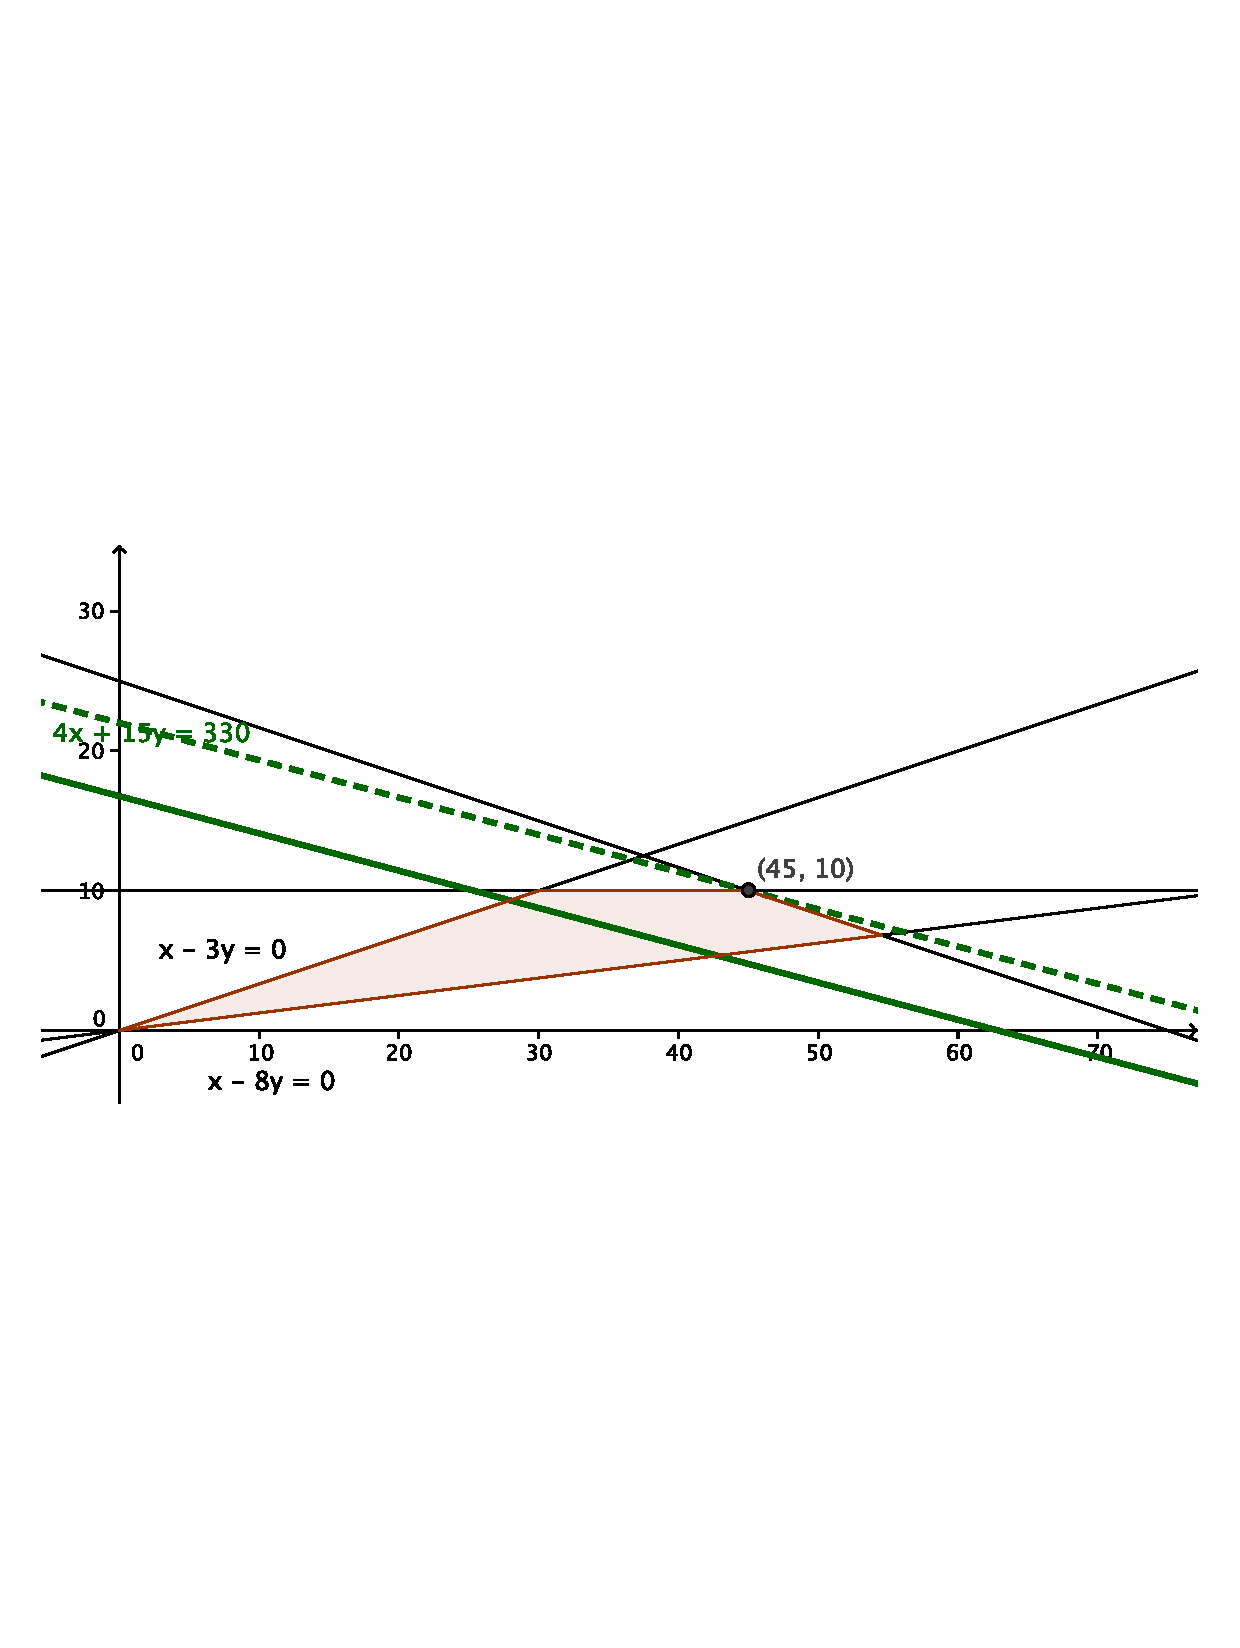
\includegraphics[width=0.8\textwidth]{oefeningen/FigurenLP/Oefautosbussen.pdf}
\caption{Maximale parkingopbrengst bij 45 auto's en 10 bussen}
\label{fig:autobussen}
\end{figure}
\end{opl}
\end{oef}

\begin{oef}
Voor een sponsoractie op school vult Anne potjes met vanille- en chocoladepudding. 
Haar moeder heeft 40 potjes die ze kan vullen 
(maar ze moeten niet allemaal gevuld worden).
Anne heeft de juf beloofd om minstens 25 potjes mee te brengen.
Ze denkt dat meer mensen vanillepudding lusten dan chocoladepudding,
dus vult ze minstens evenveel potjes met vanille als chocolade.
Vanillepudding afwerken vraagt dubbel zoveel tijd als chocoladepudding
afwerken. Anne heeft tijd om 70 potjes chocoladepudding af te werken.
Ze verkoopt de potjes vanillepudding aan \euros{1} het stuk en de 
chocoladepudding aan \euros{0,80}.
Hoeveel potjes moet Anne van elk verkopen om zoveel mogelijk
opbrengst te bekomen? 
\begin{opl}
Als Anne 30 potjes vanille- en 10 potjes chocoladepudding maakt en verkoopt (figuur~\ref{fig:pudding}) heeft ze een maximale opbrengst van \euros{38}.
\begin{figure}[hbtp]
\centering
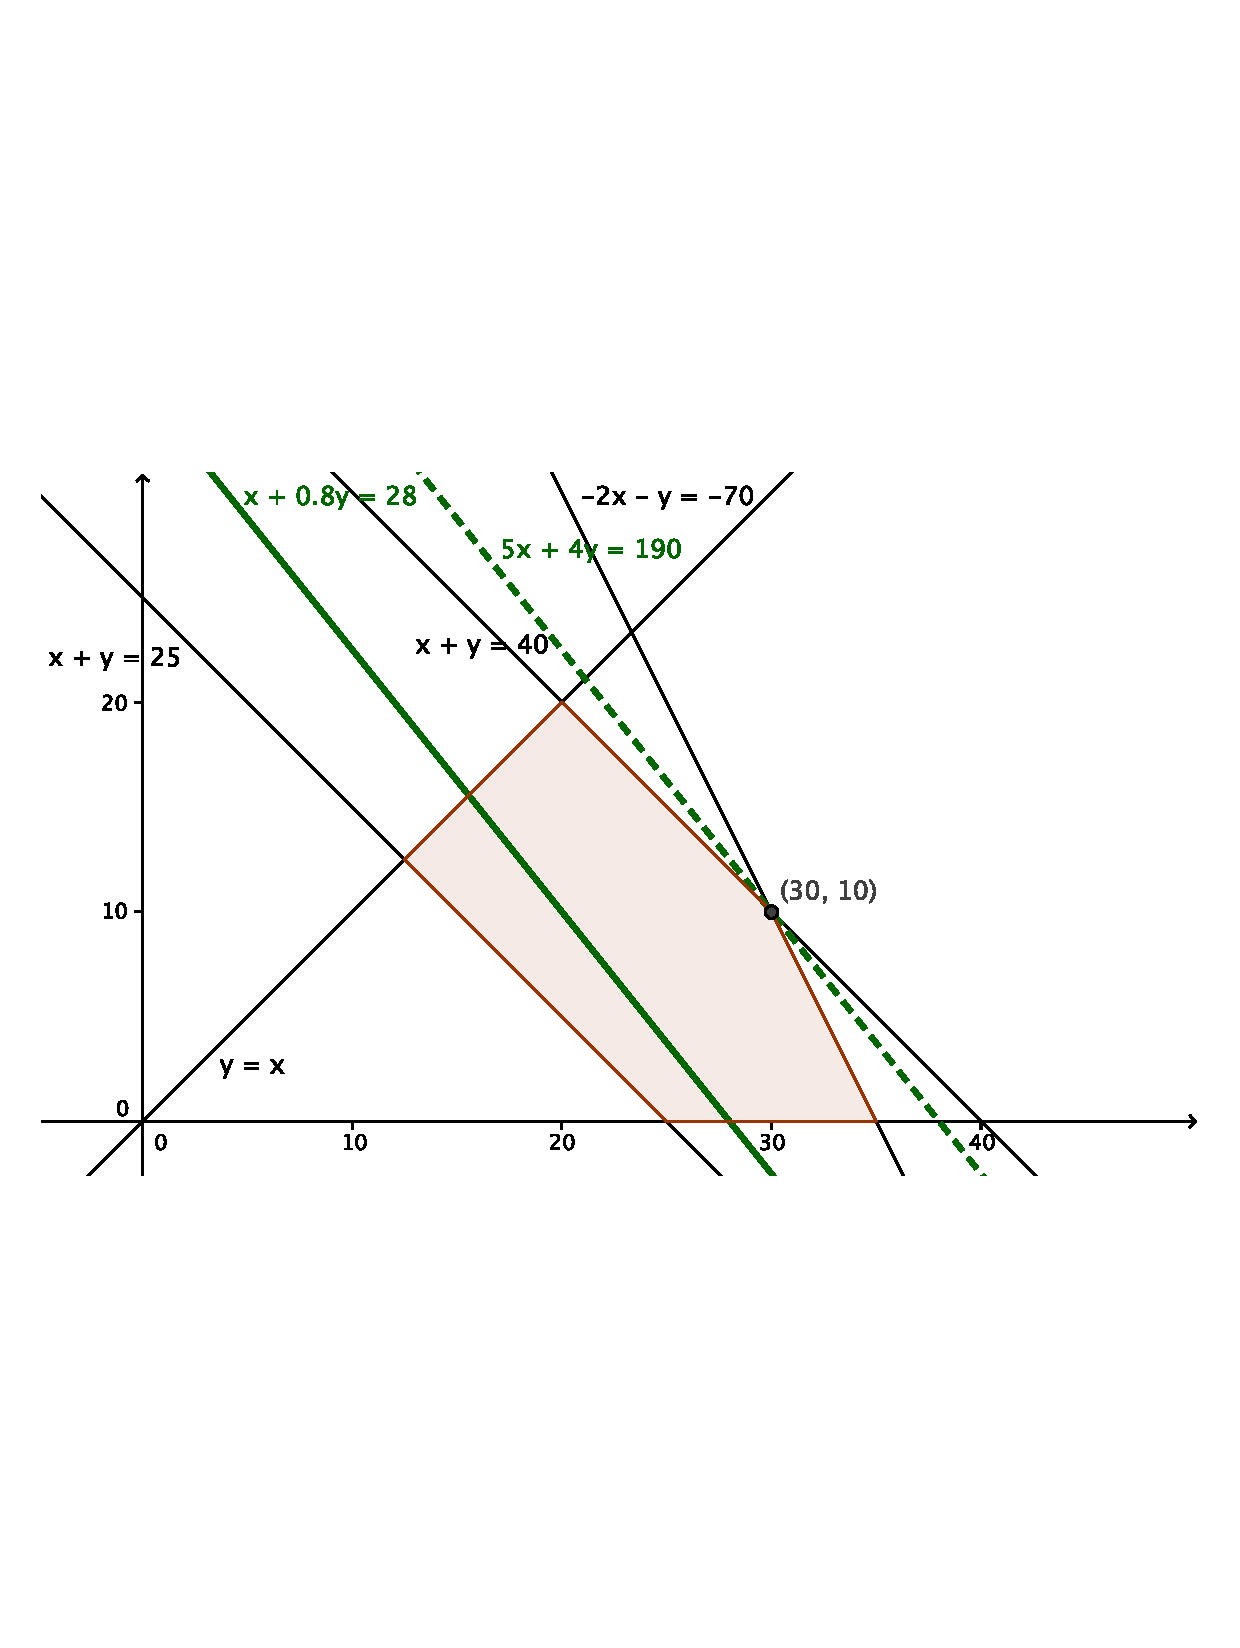
\includegraphics[width=0.8\textwidth]{oefeningen/FigurenLP/Oefpudding.pdf}
\caption{Maximale winst bij 30 potjes vanille- en 10 chocoladepudding}
\label{fig:pudding}
\end{figure}
\end{opl}
\end{oef}

\begin{oef}
Een houthakker kapt in het bos vogelkers en eik. 
De houthakker mag niet zoveel kappen als hij wil. De bosgroep hanteert
daarvoor een puntensysteem. Per ha mag er maar voor maximaal 21 punten
gehakt worden. Een vogelkers is 1 punt waard; een eik 3 punten.
Het bos is 5 ha groot.
Een eik is makkelijker te kappen dan een vogelkers. Als de houthakker per dag maar 
\'e\'en soort zou kappen, zou hij op \'e\'en dag 4 vogelkersen of 6 eiken kappen. 
Hij kan maximaal 10 dagen gaan werken in het bos.
Per eik mag de houthakker hoogstens 3 vogelkersen vellen.
Het aantal vogelkers moet minstens \'e\'en derde van het totaal aantal bomen
tellen.
Een eik geeft 10 keer zoveel winst als een vogelkers. Hoeveel bomen van elk soort
moet de houthakker kappen om zo veel mogelijk winst te bekomen? 
\begin{opl}
15 vogelkers, 30 eiken
\end{opl}
\end{oef}

\begin{oef}    
Een bouwbedrijf specialiseerde zich in het verbouwen van oude panden tot stijlvolle lofts en in de bouw van casco 1-slaapkamer appartementen. Het bedrijf heeft jaarlijks een budget van \SI{20000000}{\euro}. Om dit bedrag te kunnen lenen bij de bank moeten ze garanderen om minstens 10 appartementen en 50 lofts te realiseren. De bouw van een loft kost \SI{200000}{\euro}, een appartement is een stuk goedkoper, dit kost het bedrijf slechts \SI{100000}{\euro}. Het bouwbedrijf werkt nauw samen met een grote algemene aannemer. Deze aannemer kan maximaal personeel leveren voor de bouw van 60 lofts of 135 appartementen. De lofts kunnen anno 2013 verkocht worden aan \SI{300000}{\euro}. Voor een appartementje kan het bedrijf rekenen op een verkoopprijs van \SI{160000}{\euro}. Hoeveel lofts en appartementen moet het bedrijf realiseren en verkopen om zijn winst te maximaliseren?
\begin{opl}
50 lofts en 22 appartementen (eigenlijk 22,5 appartementen, maar je kan geen half appartement bouwen)
\begin{figure}[htb]
\centering
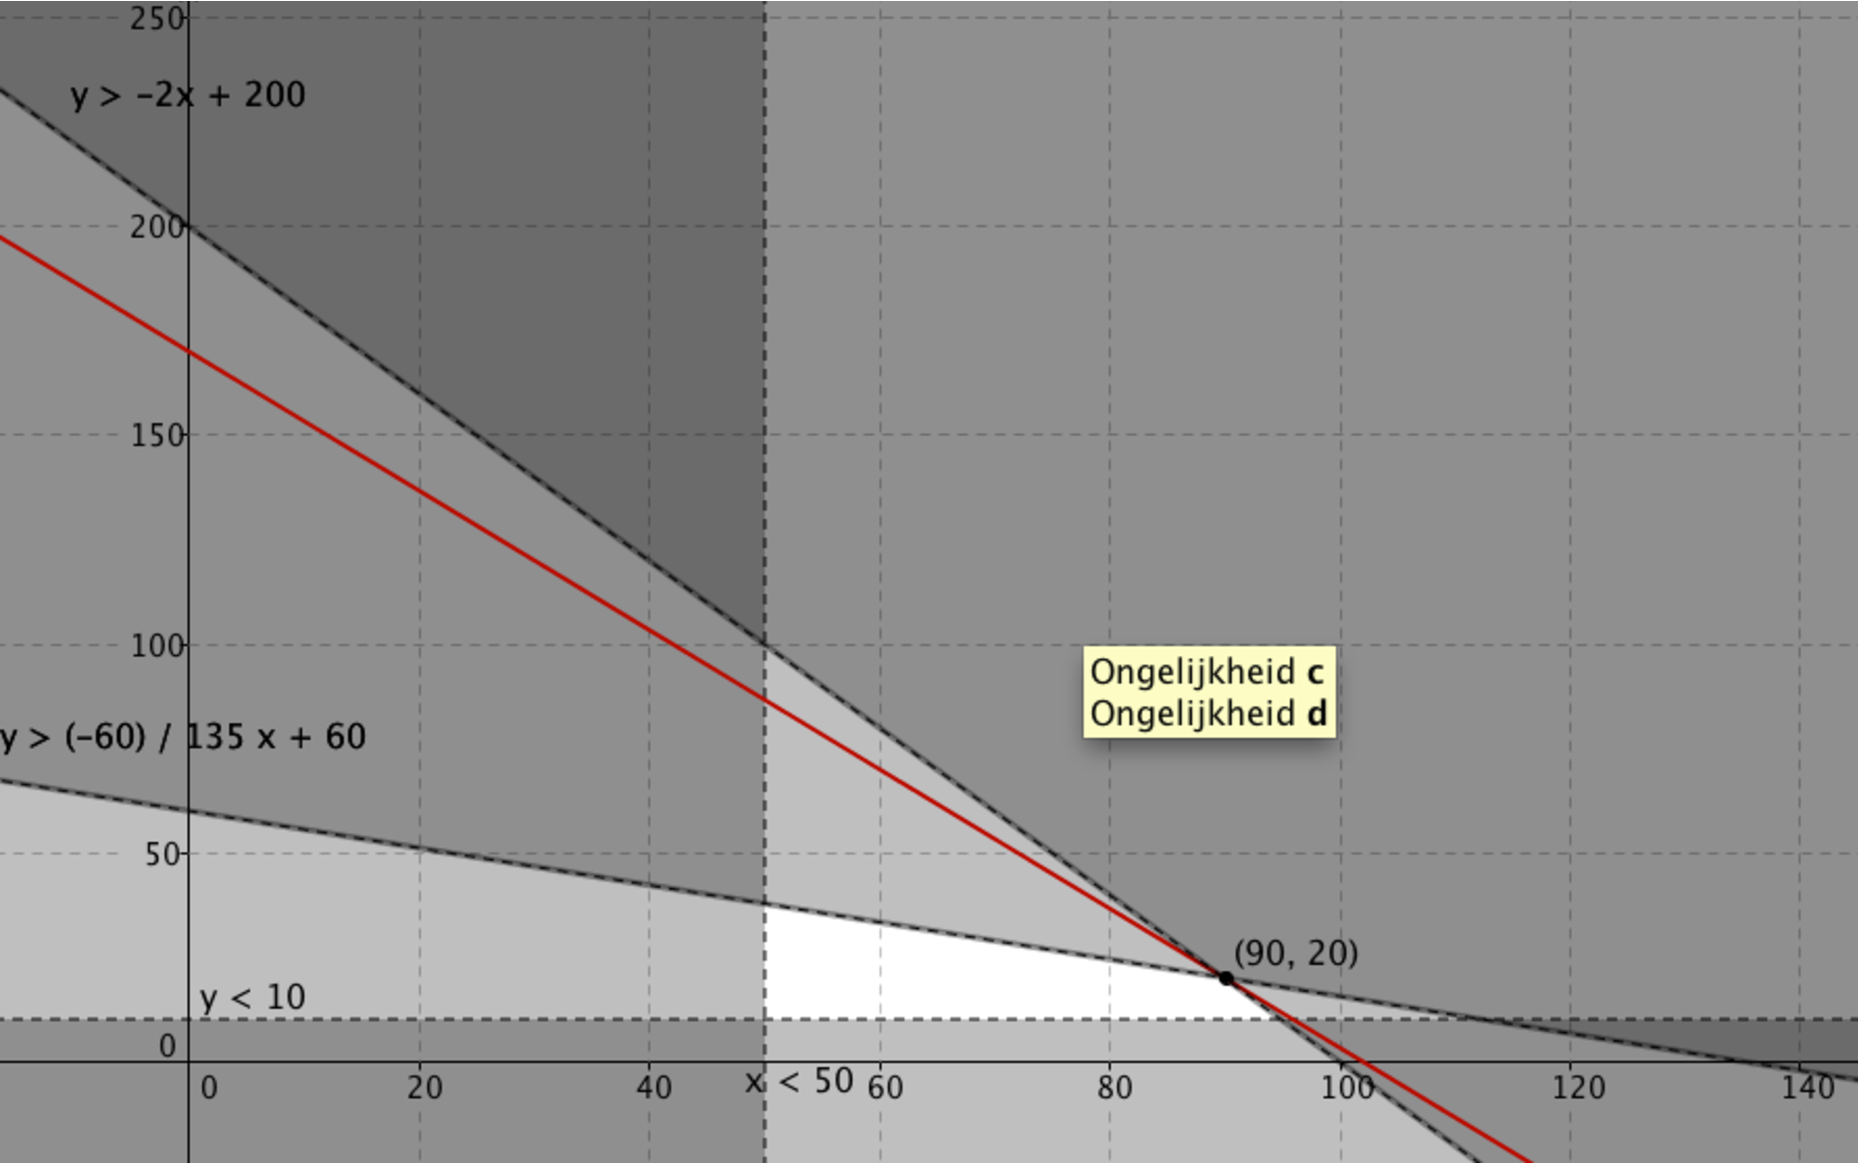
\includegraphics[width=0.8\textwidth]{oefeningen/FigurenLP/lofts}
\end{figure}
\end{opl}
\end{oef}



%\end{document}

\newpage 
%%%%%%%%%%%%%%%%%%%%%%%%%%%%%%%%%%%%%%%%%%%%%%%%%
% Laatste aanpassing:
% 6 sept 2013 [Jan]: kleine foutjes en lay-out verbeterd
%                           
% 11/9/2012 [Greetje] aangepast aan hoofdstuk eerstegraadsfuncties
% mei 2011 [Jan]: Figuren in TikZ, tabellen in booktabs, enkele foutjes verbeterd, voor eenheden siunitx gebruikt, getallen met decimale punt in \num 
%
% 23/03/11 [Greetje]: Volledige herwerking
%
% 19/9/02 [Jan]: figuur van lin. en exp. groei opnieuw
%	gemaakt (fig_ weggedaan in de naam van het bestand).
%                   
% 9/9/02 [Jan]: figuren in aparte map. Verwijzingen naar Mathcad
%    weggewerkt.
%                                               
% 04/08/02 door Roby                            
%   tekeningen aangepast aan Euler 
%             
% 10/09/01 door Greetje                         
%   typfouten van Roby vervangen                
%   $m$ uniform vervangen door \SI{•}{•}m                
%   \vspace{0.3cm} tussen caption en tabel 
%     
% 01/09/01 door Greetje                         
%%%%%%%%%%%%%%%%%%%%%%%%%%%%%%%%%%%%%%%%%%%%%%%%%



\chapter{Exponenti\"{e}le groeiprocessen}\label{chap:groei}
\begin{quote}
     \textit{{\small `Vreemderder en vreemderder!' riep Alice. (Ze was zo stomverbaasd
              dat ze eventjes compleet vergeten was hoe je ook alweer goed
              Nederlands sprak.) `Nu schuif ik uit als de grootste telescoop die
              er ooit geweest is! Vaarwel voeten!' (Want toen ze neerkeek op haar
              voeten waren ze bijna uit zicht, leek het wel, zo ver raakten ze
              weg.) `Ach, mijn arme voetjes, ik vraag me af wie jullie nu moet
              helpen bij het aantrekken van schoenen en kousen, schatten van me.
              \emph{Ik} kan het vast niet meer! Ik sta er veel te ver van af om
              me nog druk te maken over jullie. Maak er het beste van' -- maar
              ik moet aardig tegen ze zijn, dacht Alice, anders lopen ze niet
              de kant op die ik wil! Eens even denken: voortaan krijgen ze met
              de kerst nieuwe laarzen van me.}}

          Uit `Alice in Wonderland' -- Lewis Carroll
\end{quote}

\newpage
\section{Groeiprocessen: een voorbeeld}
In deze sectie behandelen we enkele modellen van groei. Het eenvoudigste model, dat in de natuur zelden voorkomt, is dat van lineaire groei. Hierbij is de aangroei per tijdseenheid constant. Meer re\"eel is het exponentieel groeimodel, waarbij de procentuele aangroei constant is. We beginnen met een voorbeeld.

\label{page:meeralgen}
\begin{quote}
    Een meer is nu \SI{800}{\square\meter} groot. Elke week wordt er \SI{550}{\square\meter} uitgegraven, zodat de oppervlakte van het meer steeds
toeneemt. Men wil het meer voor recreatie gebruiken, maar nu zijn
er reeds \SI{5}{\square\meter} algen aan de oppervlakte aanwezig. Men schat
dat de oppervlakte algen per week verdubbelt. De uitbater vindt
dat er dringend moet ingegrepen worden, maar de burgemeester ziet
geen probleem aangezien het meer ook elke week groter wordt.
Zal er steeds een gedeelte van het meer algenvrij blijven of niet?
\end{quote}
Dit voorbeeld bevat twee verschillende groeiprocessen: de aangroei van de
oppervlakte van het meer en de aangroei van de oppervlakte bedekt met algen.
We gaan na op welke manier beide processen van mekaar verschillen.

\subsection{Lineaire groei}
We bekijken eerst de groei van de oppervlakte van het meer. Zoals we gedaan hebben in \cref{chap:eerstegraadsfuncties} stellen we eerst het wiskundig model op. 
De oppervlakte benoemen we met de functie $M(t)$, met $t$ de veranderlijke tijd, uitgedrukt in weken.
Van deze functie weten we het volgende:

\begin{itemize}
  \item  Als $t=0$ dan is $M(0)=800$
  \item  Als $t=1$ dan is $M(1)=800+1\cdot 550=1350$
  \item  Als $t=3$ dan is $M(3)=800+3\cdot 550=2450$
  \item  \ldots
\end{itemize}

Dit wordt weergegeven in \cref{tabel:meer} (vergelijk met \cref{tbl:taxi} op pagina~\pageref{tbl:taxi}).
 \begin{table}[htb]
    \centering
    \vspace{0.3cm}
        \caption{De groei van de oppervlakte  van het meer.}
\begin{tikzpicture}
\node at (1.5,3) {$t$};
\node at (3,3)  {0};
\node at (5,3)  {1};
\node at (7,3)  {2};
\node at (9,3)  {3};
\node at (1.5,2)  {$M(t)$};
\node (M1) at (3,2)  {800};
\node (M2) at (5,2)  {1350};
\node (M3) at (7,2)  {1900};
\node (M4) at (9,2)  {2450};
\draw (1,2.5) -- (9.5,2.5);
\draw (2.2,1.8) -- (2.2,3.2	);
\draw[-latex] (M1) to [bend right]  node [below] {$+550$} (M2);
\draw[-latex] (M2) to [bend right]  node [below] {$+550$} (M3);
\draw[-latex] (M3) to [bend right]  node [below] {$+550$} (M4);
\end{tikzpicture}
\label{tabel:meer}
 \end{table}
 
\noindent
Hieruit leiden we  het voorschrift voor de functie $M(t)$ af.
\begin{displaymath}
    M(t)=800+t\cdot 550
\end{displaymath}
Dit is de vergelijking van  een eerstegraads- of lineaire functie. Elke week wordt  eenzelfde hoeveelheid oppervlakte \emph{opgeteld}. We spreken van \emph{lineaire groei}\index{lineaire groei}. We nemen aan dat de graafmachines de hele dag doorwerken (ook 's nachts). De veranderlijke $t$ hoeft dus geen geheel getal te zijn, maar kan een willekeurig positief reëel getal zijn. Het domein van de functie $M(t)$ is dus $\real^+$. 


Het volgend verband is onmiddellijk duidelijk:
\begin{displaymath}
    M(t)=M(t-1) +550
\end{displaymath}
 Dit verband noemen we \emph{recursief}\index{recursief}, omdat de hoeveelheid van deze  week $M(t)$ uitgedrukt wordt in functie van de hoeveelheid van de vorige week $M(t-1)$.

De grafiek van de functie $M(t)$ is een rechte (zie \cref{fig:lingroei}). Het getal $550$ is de richtingsco\"effici\"ent van de rechte. De grafiek snijdt de verticale as in $800$ (de beginwaarde $M(0)$ van het groeiproces).   Deze grafiek is typisch voor elk lineair groeiproces (vergelijk met \cref{subsec:grafischeVoorstelling}).
\begin{figure}[tbp]
    \centering
\begin{tikzpicture}[line cap=round,line join=round,x=1.0cm,y=0.0015cm]
\draw[->] (0,0) -- (5,0) node [at end, below] {$t$};
\foreach \x in {1,2,3,4}
\draw[shift={(\x,0)}] (0pt,2pt) -- (0pt,-2pt) node[below] {\footnotesize $\x$};
\draw[->] (0,0) -- (0,3500) node [at end, left] {$M(t)$};
\foreach \y in {1000,2000,3000}
\draw[shift={(0,\y)},color=black] (2pt,0pt) -- (-2pt,0pt) node[left] {\footnotesize $\y$};
\draw[color=black] (0pt,-10pt) node[right] {\footnotesize $0$};
%\clip(-0.52,0) rectangle (5.1,3900);
\draw [domain=-0:4,thick] plot(\x,{(--800--550*\x)/1});
\draw [dashed, gray] (2,0) |- (0,1900);
\draw [dashed, gray] (3,0) |- (0,2450);
\draw[-latex,red] (2,1900) to node[below] {$+1$} (3,1900) ;
\draw[-latex,red] (3,1900) to node[right] {$+550$} (3,2450) ;
\end{tikzpicture}
    \caption{Aangroei van de oppervlakte van het meer $M(t)=800+t\cdot 550$}
    \label{fig:lingroei}
\end{figure}

\subsection{Exponenti\"{e}le groei}
\label{subsec:exp_groei_vb}
We herhalen hetzelfde voor de groei van de algen. We
noemen de groeifunctie $A(t)$,
met $t$ de tijd uitgedrukt in weken.
Van deze functie weten we het volgende:
\begin{itemize}
    \item  Als $t=0$ dan is $A(0)=5$

    \item  Als $t=1$ dan is $A(1)=5\cdot 2=10$

    \item  Als $t=2$ dan is $A(2)=A(1)\cdot 2=(5\cdot 2)\cdot 2=5\cdot 2^{2}$

    \item  Als $t=3$ dan is $A(3)=A(2)\cdot 2=(5\cdot 2^{2})\cdot 2=5\cdot 2^{3}$

    \item  \ldots
\end{itemize}
Als we kijken waar we de waarde van $t$ terugvinden in de
rechteruitdrukkingen, dan vinden we als voorschrift
\begin{equation}
    A(t)=5\cdot 2^{t}
    \label{eq:algen}
\end{equation}


 \begin{table}[htb]
    \centering
        \caption{De groei van de algen  van het meer.}
\begin{tikzpicture}
\node at (1.5,3) {$t$};
\node at (3,3)  {0};
\node at (5,3)  {1};
\node at (7,3) [red]  {2};
\node at (9,3) [blue] {3};
\node at (1.5,2)  {$A(t)$};
\node (M1) at (3,2)  {5};
\node (M2) at (5,2)  {10};
\node (M3) at (7,2) [red] {20};
\node (M4) at (9,2) [blue]  {40};
\draw (1,2.5) -- (9.5,2.5);
\draw (2.2,1.8) -- (2.2,3.2	);
\draw[-latex] (M1) to [bend right]  node [below] {$\cdot 2$} (M2);
\draw[-latex] (M2) to [bend right]  node [below] {$\cdot 2$} (M3);
\draw[-latex] (M3) to [bend right]  node [below] {$\cdot 2$} (M4);
\end{tikzpicture}
\label{tabel:algen}
 \end{table}
In \cref{tabel:algen} geven we de groei schematisch weer. 

We spreken van \emph{exponenti\"ele groei}\index{exponenti\"ele groei} omdat de oppervlakte bedekt met algen elke week
\emph{vermenigvuldigd} wordt met eenzelfde factor, hier $2$. We noemen dit getal de \emph{groeifactor}. Het getal 5 geeft aan hoeveel algen er zijn op begintijdstip $t=0$. We noemen 5 dan ook de \emph{beginwaarde}.

De groei van de algen gebeurt continu:  na een halve week is de hoeveelheid reeds toegenomen. Als we er vanuit gaan dat de groeifactor de eerste helft van de week dezelfde is als de tweede helft van de week (zie \cref{fig:algen_periode2}), dan blijkt dat de veranderlijke $t$ in vergelijking~\eqref{eq:algen} geen geheel getal hoeft te zijn. Het domein van de functie $A(t)$ is dus $\real^+$.

\begin{figure}[htbp]
    \centering
\begin{tikzpicture}[x=1.5cm]
\draw[->] (-0.2,0.3) -- (7,0.3) node [at end, above] {$t$};
\foreach \x in {0,...,6}
\draw[shift={(\x,0.3)}] (0pt,1pt) -- (0pt,-2pt) node[above] {\footnotesize $\x/2$};
\node (M1) at (0,0) {5};
\node (M2) at (1,0) {$5\cdot\sqrt{2}$};
\node (M3) at (2,0) {10};
\node (M4) at (3,0) {$10\cdot\sqrt{2}$};
\node (M5) at (4,0) {20};
\node (M6) at (5,0) {$20\cdot\sqrt{2}$};
\node (M7) at (6,0) {40};
\draw[-latex] (M1) to [bend right]  node [below] {$\cdot \sqrt{2}$} (M2);
\draw[-latex] (M2) to [bend right]  node [below] {$\cdot \sqrt{2}$} (M3);
\draw[-latex,color=red,thick] (M1) to [out=-60,in=-120]  node [below] {$\cdot 2$} (M3);
\draw[-latex] (M3) to [bend right]  node [below] {$\cdot \sqrt{2}$} (M4);
\draw[-latex] (M4) to [bend right]  node [below] {$\cdot \sqrt{2}$} (M5);
\draw[-latex,color=red,thick] (M3) to [out=-60,in=-120]  node [below] {$\cdot 2$} (M5);
\draw[-latex] (M5) to [bend right]  node [below] {$\cdot \sqrt{2}$} (M6);
\draw[-latex] (M6) to [bend right]  node [below] {$\cdot \sqrt{2}$} (M7);
\draw[-latex,color=red,thick] (M5) to [out=-60,in=-120]  node [below] {$\cdot 2$} (M7);
\end{tikzpicture}
    \caption{Groeifactor van de aangroei van de algen verandert als de periode verandert }
    \label{fig:algen_periode2}
\end{figure}

Het volgend verband is voor iedereen onmiddellijk duidelijk:
\[A(t)=A(t-1)\cdot 2
\] 
Dit is opnieuw een \emph{recursief}\index{recursief} voorschrift.

Zoals je ziet op \cref{fig:algen}, is de grafiek van $A(t)$ geen rechte meer. Omdat de veranderlijke $t$
in vergelijking~\eqref{eq:algen} in de exponent staat noemen we $A(t)$  een \emph{exponenti\"{e}le
functie}. De groeifactor $2$ is het grondtal\index{grondtal} van de exponenti\"ele functie.
De beginwaarde $5$ is het snijpunt van de functie met de verticale as. In \cref{chap:expFunctie} gaan we dieper in op exponentiële functies.
\begin{figure}[tbp]
    \centering
    \begin{tikzpicture}[line cap=round,line join=round,x=1.0cm,y=0.05cm]
    \draw[->] (-2.2,0) -- (5.5,0) node [at end, below] {$t$};
    \foreach \x in {-1,0,1,2,3,4,5}
    \draw[shift={(\x,0)}] (0pt,2pt) -- (0pt,-2pt) node[below] {\footnotesize $\x$};
    \draw[->] (0,0) -- (0,170) node [at end, left] {$A(t)$};
    \foreach \y in {20,40,...,160}
    \draw[shift={(0,\y)},color=black] (2pt,0pt) -- (-2pt,0pt) node[left] {\footnotesize $\y$};
    \draw [domain=-2:5,thick] plot(\x,{5*exp(\x*ln(2))});
    \draw [dashed, gray] (2,0) |- (0,20);
    \draw [dashed, gray] (3,0) |- (0,40);
        \filldraw [red] (2,20) circle (2pt);
            \filldraw [blue] (3,40) circle (2pt);
    \end{tikzpicture}
    \caption{Aangroei van de oppervlakte bedekt met algen $A(t)=5\cdot 2^{t}$}
    \label{fig:algen}
\end{figure}


\subsection{Vergelijking van de twee groeiprocessen.}
\begin{figure}[tbp]
    \centering
\begin{tikzpicture}[line cap=round,line join=round,x=0.8cm,y=0.0005cm]
\draw[->] (-0.2,0) -- (12,0) node [at end, below] {$t$};
\foreach \x in {0,...,11}
\draw[shift={(\x,0)}] (0pt,2pt) -- (0pt,-2pt) node[below] {\footnotesize $\x$};
\draw[->] (0,0) -- (0,16000) node [at end, left] {$y$};
\foreach \y in {2000,4000,6000,8000,10000,12000,14000}
\draw[shift={(0,\y)},color=black] (2pt,0pt) -- (-2pt,0pt) node[left] {\footnotesize $\y$};
\draw [domain=0:11.5,thick,color=red] plot(\x,{5*exp(\x*ln(2))});
\draw [domain=-0:11.5,thick,color=blue] plot(\x,{(--800--550*\x)/1});
\draw [dashed, gray] (10.34,0) |- (0,6488);
\node at (11,15000) [red] {$A(t)$};
\node at (11.5,7600) [blue] {$M(t)$};
    \filldraw [black!60] (10.34,6488) circle (2pt);
\end{tikzpicture}
    \caption{Aangroei van de oppervlakte van het meer $M(t)=800+t\cdot 550$ en aangroei van de oppervlakte bedekt met algen $A(t)=5\cdot 2^{t}$}
    \label{fig:linexp}
\end{figure}

In \cref{fig:linexp} vind je de grafieken van $A(t)$ en
$M(t)$ op \'{e}\'{e}n tekening. We zien duidelijk
dat de groei van de oppervlakte bedekt met algen
in het begin traag gaat, want er zijn weinig algen. Zodra
er meer algen zijn, groeien die veel sneller aan en zullen ze
het ganse meer overwoekeren. Op de grafiek lezen we af dat
tussen de $10$ en de $11$ weken het meer overwoekerd is door algen.
Dezelfde oplossing lezen we af op
\cref{tbl:meeralgen}, waar de resultaten per week van beide
groeiprocessen weergegeven worden.
\begin{table}[htb]
    \centering
    \caption{De groei van de algen en de oppervlakte van het meer.}
    \begin{tabular}{rrcr}
    \toprule
    $t$ & $A(t)$ & verband & $M(t)$  \\
    \midrule
    0 & 5 & ${\color{red}<}$ & 800  \\
    1 & 10 & ${\color{red}<}$ & 1350  \\
    2 & 20 & ${\color{red}<}$ & 1900  \\
    3 & 40 &  ${\color{red}<}$ & 2450  \\
    4 & 80 &  ${\color{red}<}$ & 3000  \\
    5 & 160 &  ${\color{red}<}$ & 3550  \\
    6 & 320 &  ${\color{red}<}$ & 4100  \\
    7 & 640 &  ${\color{red}<}$ & 4650  \\
    8 & 1280 &  ${\color{red}<}$ & 5200  \\
    9 & 2560 & ${\color{red}<}$ & 5750  \\
    10 & 5120 &  ${\color{red}<}$ & 6300  \\
    \cmidrule{2-4}
    11 & 10240 & ${\color{blue}>}$ & 6850  \\
    12 & 20480 & ${\color{blue}>}$ & 7400 \\
    \bottomrule
\end{tabular}
    \label{tbl:meeralgen}
\end{table}

We kunnen het moment dat het meer vol algen zit ook berekenen met formules. De uitgegraven oppervlakte is gelijk aan de oppervlakte bedekt met algen als
\begin{displaymath}
    800+550\cdot t=5\cdot 2^{t}
\end{displaymath}
Deze vergelijking ziet er vrij eenvoudig uit. Nochtans kan ze niet
opgelost worden met de methoden van \cref{sec:exp_vgl}.  We kunnen ze alleen
 benaderend oplossen met de computer. Als we een algoritme zouden programmeren en dit toepassen, vinden we $t=\num{10.342}$ weken. \\
 
 \noindent
\textbf {Besluit:} Wil de burgemeester dit gebied als recreatiezone gebruiken
 dan moet hij de groei van de algen drastisch indijken.



\newpage
\section{Exponenti\"ele groei}
\subsection{Definities}

We veralgemenen vergelijking \eqref{eq:algen} van \cref{subsec:exp_groei_vb}. 
\begin{quote}

Zij  $B(t)$ de functie die de exponenti\"{e}le
aangroei van een grootheid weergeeft, waarbij $t$ uitgedrukt is in aantal \emph{perioden}\index{periode} (bijvoorbeeld weken, uren, meter, centimeter). De \emph{groeifactor}\index{groeifactor} $g$ is de factor waarmee de functie per periode toeneemt (vermenigvuldigd wordt). Bij het begin van de meting ($t=0$) heeft de functie \emph{beginwaarde}\index{beginwaarde} $B(0)$. Dan is het functievoorschrift van deze functie
\begin{equation}
    B(t)=B(0)\cdot g^{t}
    \label{eq:eq_groei2}
\end{equation}
Het domein van de functie $B(t)$ is $\real^+$.

\end{quote}
De recursieve formule is :
\begin{equation}
    B(t)=B(t-1)\cdot g
\end{equation}
want $g$ is \emph{onafhankelijk} van het moment waarop men de periode laat
beginnen.



De groeifactor is \emph{wel} afhankelijk van de
lengte van de periode. We nemen terug het voorbeeld van \cref{subsec:exp_groei_vb}.  In het voorbeeld wordt de aangroei \emph{per week}  bekeken: week na week moet je de hoeveelheid algen vermenigvuldigen met twee (periode: 1 week; groeifactor: 2). Wat als je de aangroei van de algen per 3 weken wil meten (periode: 3 weken)? In \cref{fig:algen_periode} zie je dat in dat geval de hoeveelheid algen per periode drie keer na mekaar met 2 vermenigvuldigd moet worden, dus met $2^3=8$. Als de periode 3 weken bedraagt, is de groeifactor gelijk aan 8.
\begin{figure}[htbp]
    \centering
\begin{tikzpicture}[x=1.5cm]
\draw[->] (-0.2,0.3) -- (7,0.3) node [at end, above] {$t$};
\foreach \x in {0,...,6}
\draw[shift={(\x,0.3)}] (0pt,1pt) -- (0pt,-2pt) node[above] {\footnotesize $\x$};
\node (M1) at (0,0) {5};
\node (M2) at (1,0) {10};
\node (M3) at (2,0) {20};
\node (M4) at (3,0) {40};
\node (M5) at (4,0) {80};
\node (M6) at (5,0) {160};
\node (M7) at (6,0) {320};
\draw[-latex] (M1) to [bend right]  node [below] {$\cdot 2$} (M2);
\draw[-latex] (M2) to [bend right]  node [below] {$\cdot 2$} (M3);
\draw[-latex] (M3) to [bend right]  node [below] {$\cdot 2$} (M4);
\draw[-latex,color=red,thick] (M1) to [out=-60,in=-120]  node [below] {$\cdot 8$} (M4);
\draw[-latex] (M4) to [bend right]  node [below] {$\cdot 2$} (M5);
\draw[-latex] (M5) to [bend right]  node [below] {$\cdot 2$} (M6);
\draw[-latex] (M6) to [bend right]  node [below] {$\cdot 2$} (M7);
\draw[-latex,color=red,thick] (M4) to [out=-60,in=-120]  node [below] {$\cdot 8$} (M7);
\end{tikzpicture}
    \caption{Groeifactor van de aangroei van de algen verandert als de periode verandert }
    \label{fig:algen_periode}
\end{figure}

In het algemeen komt het op het volgende neer: als je de periode vermenigvuldigt met een factor $k$, moet je de groeifactor tot de $k$-de macht verheffen. Dit wordt schematisch weergegeven in \cref{fig:periode_factor}.
\begin{figure}[tbp]
    \centering
\begin{tikzpicture}[x=1.5cm]
\draw[dashed](3.5,0.0)--(4.5,0.0);
\draw[] (-0.2,0.0) -- (3.5,0.0);
\draw[->] (4.5,0.0) -- (5.3,0.0) node [at end, above] {$t$};
\foreach \x in {0,1,2,3}
\draw[shift={(\x,0.0)}] (0pt,1pt) -- (0pt,-2pt) node[above] {\footnotesize $\x$};
\draw[shift={(5,0.0)}] (0pt,1pt) -- (0pt,-2pt) node[above] {\footnotesize $k$};
\node (M1) at (0,0) {};
\node (M2) at (1,0) {};
\node (M3) at (2,0) {};
\node (M4) at (3,0) {};
\node (Mk) at (5,0) {};
\draw[-latex] (M1) to [bend right]  node [below] {$\cdot g$} (M2);
\draw[-latex] (M1) to [bend left]  node [above] {$+1$} (M2);
\draw[-latex,color=red,thick] (M1) to [out=-50,in=-130]  node [below] {groeifactor $= g^k$} (Mk);
\draw[-latex,color=red,thick,dashed] (M1) to [out=50,in=130]  node [above] {periode $p=k$} (Mk);
\end{tikzpicture}
    \caption{Relatie tussen periode $p$ en groeifactor}
    \label{fig:periode_factor}
\end{figure}
Als de periode kleiner wordt, is de factor $k$ kleiner dan 1. Als in het algenprobleem de periode gelijk is aan 1 dag (=1/7 van een week), is de groeifactor $2^{1/7}$.

In elk probleem is de
keuze van de periode vrij te kiezen, maar de groeifactor zal door die
keuze bepaald worden.\\


We besluiten: een exponentieel groeiproces wordt gekenmerkt door drie elementen:
\begin{enumerate}
\item de beginwaarde $K(0)$
\item de periode $p$
\item de groeifactor $g$
\end{enumerate}
Het functievoorschrift van het groeiproces is dan 
\begin{equation}
K(t)=K(0)\cdot g^t
\label{eq:exp_groei}
\end{equation}
Het domein van het groeiproces is $\real^+$.
Merk op dat de veranderlijke $t$ niet steeds een tijd is. De veranderlijke kan ook een afstand zijn, de diepte, de hoogte \dots.

Vaak worden opeenvolgende metingen van een experiment gebruikt om de toestand van de opstelling te achterhalen  \emph{voor} het begin van de meting. Als het zinvol is, kan de veranderlijke $t$ dan een negatieve waarde aannemen. 

\subsection{Stijgend groeiproces}\label{subsec:stijgendGroeiproces}
In het voorbeeld van \cref{subsec:exp_groei_vb} neemt de grootheid $A(t)$ toe in de tijd: de
oppervlakte bedekt met algen wordt steeds groter. We noemen dit dan
ook een stijgend groeiproces. In wat volgt geven we nog een voorbeeld van een stijgend
groeiproces. 

\subsubsection{Voorbeeld: samengestelde intrest}\label{subsubsec.si}
Als je geld stort op je spaarboekje, krijg je vanaf de eerste dag reeds intrest. Deze intrest wordt bij het kapitaal geteld en brengt op zijn beurt opnieuw intrest op. Dit noemen we samengestelde intrest.
\begin{quote}
    Een kapitaal van \euros{1000} staat gedurende 10 jaar uit tegen een
jaarlijkse rentevoet van \SI{7}{\percent}. Hoe groot is dit kapitaal na 10
jaar?
\end{quote}
Is het hierboven beschreven proces inderdaad een exponentieel groeiproces? 
We noemen de functie die het kapitaal
weergeeft in functie van de tijd $K(t)$, met $t$ uitgedrukt in jaren.
In \cref{tbl:groeikap} berekenen we het kapitaal voor drie opeenvolgende jaren.
\begin{table}[tbp]
    \centering
    \caption{De groei van het kapitaal per jaar}
    \begin{tabular}{ll}
    \toprule
    $t$ & $K(t)$\\
    \midrule
    $0$ 	& $K(0)=1000$ 	\\
    $1$	&$K(1)=K(0)+K(0)\cdot \num{0.07}=  K(0)\cdot \num{1.07}=1070$\\
   $2$	&$K(2)=K(1)+K(1)\cdot \num{0.07}= K(1)\cdot \num{1.07}=\num{1144.9}$ \\
   $3$	&$K(3)=K(2)+K(2)\cdot \num{0.07}= K(2)\cdot \num{1.07}=\num{1225.043}$ \\
\bottomrule
\end{tabular}
\label{tbl:groeikap}
\end{table}
Als we in deze tabel alle getallen samenvatten op een tijdsas bekomen we \cref{fig:kapitaalgroei}.
\begin{figure}[htbp]
    \centering
\begin{tikzpicture}[x=2cm]
\draw[->] (-0.2,0) -- (3.5,0) node [at end, above] {$t$};
\foreach \x/\y in {0/1000,1/1070,2/\num{1144.9},3/\num{1225.043}}{
	\draw[shift={(\x,0.0)}] (0pt,1pt) -- (0pt,-2pt) node[above] {\small $\x$};
	\node (\x) [below] at (\x,0) {\y};
}
\foreach \x/\y in {0/1,1/2,2/3}
	\draw[-latex] (\x) to [bend right]  node [below] {$\cdot 1,07$} (\y);
\end{tikzpicture}
    \caption{Groei van kapitaal van \euros{1000} tegen een WR van \SI{7}{\percent}}
    \label{fig:kapitaalgroei} 
\end{figure}



We merken het volgende:
\begin{enumerate}
\item De beginwaarde is gelijk aan $K(0)=1000$.
\item Uit de opgave blijkt dat de periode gelijk is aan 1 jaar.
\item Jaar na jaar wordt het kapitaal vermenigvuldigd met $\num{1.07}$. De groeifactor $g$ is dus gelijk aan \num{1.07}.
\end{enumerate}
Het hierboven beschreven proces is inderdaad een exponentieel groeiproces. Uit vergelijking~\eqref{eq:exp_groei} volgt dat het voorschrift gegeven is door 
\begin{equation}
     K(t)=K(0)\cdot g^{t}=1000\cdot \num{1.07}^{t}
    \label{eq:si}
\end{equation}

Om het kapitaal na 10 jaar te berekenen, hoeven we enkel $K(10)=1000\cdot \num{1.07}^{10}=1967,15$ te berekenen. We vinden een kapitaal van \euros{1967,15}.

\subsubsection{Procentuele toename}
Hoe verandert de absolute toename $V(t)=K(t)-K(t-1)$ per periode (tijdseenheid) in een
exponentieel groeiproces?  We berekenen enkele van die toenamen in
\cref{tbl:samgesint} (derde kolom). 
\begin{table}[htb]
    \centering
    \caption{De \emph{toename} van het kapitaal per jaar}
    \begin{tabular}{cccc}
     \toprule
    $t$ & $K(t)$ & $V(t)=K(t)-K(t-1)$  & $ P(t)=\dfrac{V(t)}{K(t-1)}$\\
    \midrule
    0 & 1000 &   &\\

    1 & 1070 & 70&$\dfrac{70}{1000}=\num{0.07}$   \\[10pt]

    2 & \num{1144,9} & \num{74,9} & $\dfrac{\num{74.9}}{1070}=\num{0.07}$  \\[10pt]

    3 & \num{1225,043} & \num{80,14} &$\dfrac{\num{80.14}}{\num{1144.9}}=\num{0.07}$ \\[10pt]

    4 & \num{1310,796} & \num{85,75}  & $\dfrac{\num{85,75}}{\num{1225,043}}=\num{0.07}$\\
    \bottomrule
\end{tabular}
    \label{tbl:samgesint}
\end{table}

Uit \cref{tbl:samgesint}  blijkt dat de absolute toename jaar na jaar toeneemt. Dit is typisch voor een exponentieel groeiproces. 
 Bij lineaire groei is deze absolute toename constant. Daardoor is de grafiek van een lineair groeiproces een rechte en die van een exponentieel groeiproces niet.
 
 Berekenen we echter de
 \emph{procentuele jaarlijkse toename} $P(t)$,  de verhouding van de
 absolute toename $V(t)$ tot het kapitaal dat er was bij het vorige tijdstip $K(t-1)$ (vierde kolom in \cref{tbl:samgesint})
 \begin{displaymath}
     P(t)=\frac{V(t)}{K(t-1)}
 \end{displaymath}
We zien dat de procentuele toename per periode wel
constant is. De procentuele toename blijkt gelijk te zijn aan de groeifactor $g=\num{1.07}$ verminderd met 1.

We besluiten: een groeiproces met procentuele toename van $p$\,\%
per periode, heeft per tijdseenheid een groeifactor 
\begin{equation}
g=1+\frac{p}{100}
\label{eq:groeifactor_procent}
\end{equation}

\subsection{Dalend groeiproces}\label{subsec.ballon}
Tot nog toe zagen we enkel voorbeelden van stijgende groeiprocessen: de bijbehorende groeifunties waren steeds stijgend. In wat volgt bespreken we een dalend groeiproces.
\begin{quote}
    Een luchtballon verliest  \SI{5}{\percent} van zijn
    draaggas per dag omdat het omhulsel wat poreus is. Bepaal de functie die weergeeft welke de hoeveelheid draaggas is in functie van de tijd, uitgedrukt in dagen. Nu is er \SI{1000}{\milli\litre} gas aanwezig in de luchtballon.
\end{quote}


Stel $t$ de tijd, uitgedrukt in dagen gerekend
vanaf nu. De hoeveelheid draaggas op het tijdstip $t$ noemen we $D(t)$.
Elke dag moeten we \SI{5}{\percent}  van de aanwezige hoeveelheid gas
aftrekken, dus
\begin{equation}
  D(t) = D(t-1)-D(t-1)\cdot \frac{5}{100}  
\end{equation}
Dit geeft, na wat rekenwerk
\begin{equation}
   D(t)  =   D(t-1)\cdot (1-\frac{5}{100}) 
     =  D(t-1)\cdot \num{0.95}
     \label{eq:draaggas}
\end{equation}
Hieruit blijkt dat de groeifactor per  dag gelijk is aan $1-\frac{5}{100}=\num{0.95}$.  
Enkele berekende waarden van $D(t)$ en $V(t)=D(t)-D(t-1)$ vind je in
 \cref{tbl:gas}. We zien dat de absolute afname elke dag verder \emph{daalt.}
 \begin{table}[htb]
    \centering
    \caption{De \emph{toename} van het draaggas per dag}
    \begin{tabular}{cSS}
     \toprule
     t & {D(t)} & {V(t)}  \\
     \midrule
     0 & 1000 &   \\
     1 & 950 & -50  \\
     2 & \num{902.5} & \num{-47.5}  \\
     3 & \num{857.375} & \num{-45.125}  \\
     4 & \num{814.506} & \num{-42.869}  \\
     5 & \num{773.781} & \num{-40.725}  \\
     \bottomrule
 \end{tabular}
    \label{tbl:gas}
\end{table}

Het groeiproces dat de hoeveelheid draaggas in de luchtballon beschrijft wordt dus gekenmerkt door de volgende elementen:
\begin{enumerate}
  \item beginwaarde $D(0)=1000$
  \item periode $p=1$ dag
  \item groeifactor $g=\num{0.95}$
\end{enumerate}
Uit vergelijking~\eqref{eq:exp_groei} volgt  dat de functie die de hoeveelheid draaggas op tijdstip $t$ beschrijft, gegeven wordt door 
\begin{equation}
  D(t)=1000\cdot \num{0.95}^{t} \qquad\mbox{ met $t$ uitgedrukt in dagen}
  \label{eq:ballon}
\end{equation}


\subsubsection{Besluit}
Een groeiproces met een constante
procentuele afname van $p$\,\% per tijdseenheid is een dalend
exponentieel proces met als groeifactor $ g=1-\frac{p}{100}$.
Hierbij geldt voor de groeifactor: $0<g<1$.

%%%%%%%%%%%%%%%%%%%%%%%%%%%%%%%%%
% 6 sept 2013 [Jan]: kleine verbeteringen (komma's, eenheden, getallen)
% november 2012 [Greetje]: oplossingen, fout bij oef 1 en kleine wijziging in oef 2
% mei 2011 [Jan]: oefening Fukushima Jodium 131
%
% 9/4/11 [Greetje] Grondige herziening
% 
%Aanpassing greetje   %
% 10/09/01  
% verbeteringen roos    %
% 
% Laatste aanpassing:           %
% 17/08/02 door Roos
%   verbeteringen schooljaar 2001-2002
%  nieuwe oefeningen test en ex.Roby %
% 12/07/02 door Roos        %
%%%%%%%%%%%%%%%%%%%%%%%%%%%%%%%%%

% \chapter{Oefeningen op exponenti\"{e}le groei}
\section{Oefeningen}


\begin{oef}    
In tabel~\ref{tbl:6processen} vind je de functiewaarden van enkele functies. 
     Ga na of de functies overeenkomen met een
      exponentieel of een lineair proces of geen van
      beide.
      \begin{table}[htb]
                \centering
                \caption{6 verschillende groeiprocessen}
          \begin{tabular}{ccccccc}
         \toprule
         $t$ & $f(t)$ & $g(t)$ & $h(t)$ & $k(t)$ & $m(t)$ & $w(t)$ \\
         \midrule

         1 & 10 & 105 & 12 & 1701 & 5 & \num{29.7}  \\

         2 & 17 & 118 & \num{13.2} & 567 & 25 & \num{27.1}  \\

         3 & 24 & 131 & \num{14.52} & 189 & 125 & \num{24.5}  \\

         4 & 31 & 146 & \num{15.972} & 63 & 625 & \num{21.9}  \\

         5 & 38 & 163 & \num{17.5692} & 21 & 3125 & \num{19.3}  \\
         \bottomrule

     \end{tabular}
          \label{tbl:6processen}
      \end{table}
      \begin{opl}
      \begin{itemize}
      \item $f$: lineair groeiproces met toename gelijk aan 7
      \item $g$: geen exponentiële en geen lineaire groei
      \item $h$: exponentieel groeiproces met groeifactor gelijk aan 1,1
      \item $k$: exponentieel groeiproces met groeifactor gelijk aan $\frac13$
      \item $m$: exponentieel groeiproces met groeifactor gelijk aan 5
      \item $w$: lineair groeiproces met toename gelijk aan $-2,6$
      \end{itemize}
      \end{opl}
\end{oef}

\begin{oef}
 
    
        Het aantal microben in een proefopstelling verdubbelt in 6
     uren tijd.
     \begin{enumerate}
         \item  Wat is de groeifactor (i) per 6 uur? (ii) per dag? (iii) per uur?

         \item  Veronderstel dat het aantal microben nu 100 bedraagt. Bereken zonder rekenmachine en zonder functievoorschrift, indien mogelijk, wanneer het er (i) 400 zijn, (ii) 25,  (iii) 1000.

         \item  Geef het functievoorschrift voor dit groeiproces met als periode
          (i) \'e\'en dag, (ii)  6 uur, (iii) \'{e}\'{e}n uur. Neem 100 als beginwaarde.
          
          \item Maak in Scilab de grafiek van \'e\'en van de functievoorschriften die je hierboven vond. Lees op de grafiek af wanneer er 1000 microben zijn.
     \end{enumerate}
     \begin{opl}
     \begin{enumerate}
     \item $g_6=2$; $g_d=2^4=16$; $g_u=2^\frac{1}{6}=1,122462$
     \item (i) 12u; (ii) 12 uur geleden; (iii) tussen 18 en 24u
     \item $g_6(t)=100\cdot 2^t$; $g_d(t)=100\cdot 16^t$; $g_u(t)=100\cdot \left(2^\frac16 \right)^t$
     \end{enumerate}
     \end{opl}

      \end{oef}

\begin{oef}
  In 2011 waren er ongeveer 7 miljard mensen. Per jaar is
      de bevolkingstoename ongeveer \SI{1,1}{\percent}.
      \begin{enumerate}
          \item  Wat is de groeifactor per jaar? Per decennium? Per semester?
          
          \item Stel de vergelijking op van de groeifunctie die het aantal mensen $M(t)$ op tijdstip $t$ met $t$ uitgedrukt in jaren, weergeeft. 
          
          \item  Hoeveel mensen verwacht men in 2050 volgens dit model?

          \item Maak een grafiek van de functie in Scilab. Lees op de grafiek af wanneer  de bevolking 8 miljard zal bedragen.

      \end{enumerate}
      \begin{opl}
      \begin{enumerate}
      \item $g_j=1,011$; $g_d=1,011^{10}$; $g_s=1,011^\frac{1}{2}$
      \item $M(t)=7\cdot 1,011^t$ in miljard aantal en $t$ het aantal jaren verstreken sinds 2011
      \item $M(39)=7\cdot 1,011^{39}=10,724896$
      \end{enumerate}
      \end{opl}

      \end{oef}



\begin{oef}
 Bij een dieptetoename van \SI{32}{\meter} in de aarde vermeerdert
    de temperatuur met \SI{1}{\celsius}.
    \begin{enumerate}
    \item Veronderstel dat op een diepte van \SI{25}{\meter} een temperatuur
    van \SI{10}{\celsius} heerst.
        \begin{enumerate}
        \item Op welke diepte heerst een temperatuur van
        \SI{15}{\celsius}?
        \item Welke temperatuur heerst er op een diepte van \SI{985}{\meter}?
        \end{enumerate}
    \item Veronderstel dat op de grond (\SI{0}{\meter}) een temperatuur
    van \SI{-5}{\celsius} heerst.
        \begin{enumerate}
        \item Op welke diepte heerst een temperatuur van
        \SI{0}{\celsius}?
        \item Welke temperatuur heerst er op een diepte van \SI{800}{\meter}?
        \end{enumerate}
    \end{enumerate}
\begin{opl}
\begin{enumerate}
\item 
$T_1(t)=10+\frac{t}{32}$ met $t$ het aantal meter grond dieper dan \SI{25}{\meter} onder de grond
\begin{enumerate}
\item Zoek $t$ zodat $T_1(t)=15$: op diepte van \SI{185}{\meter} onder de grond bedraagt de temperatuur \SI{15}{\celsius}.
\item $T_1(960)=40$, dus \SI{40}{\celsius}
\end{enumerate}
\item $T_2(t)=-5+\frac{t}{32}$ met $t$ het aantal meter onder de grond
\begin{enumerate}
\item Zoek $t$ zodat $T_2(t)=0$ geeft $t=160$, dus \SI{160}{meter} onder de grond bedraagt de temperatuur \SI{0}{\celsius}
\item $T_2(800)=20$, dus \SI{800}{meter} onder de grond is het \SI{20}{\celsius}
\end{enumerate}
\end{enumerate}
\end{opl}
\end{oef}





\begin{oef}
 De hoeveelheid  radium halveert om de  1656 jaar.
    \begin{enumerate}
        \item Hoeveel vermindert de hoeveelheid radium
            procentueel per jaar?
        \item Schrijf de functie  die de hoeveelheid radium op tijdstip
            $t$ weergeeft, als de initi\"ele hoeveelheid radium $y_0$
            bedraagt, waarbij $t$ uitgedrukt is in jaren.
        \item Hoeveel gram radium blijft er over van \SI{1}{\gram} na 20
            jaar?
    \end{enumerate}
\begin{opl}
\begin{enumerate}
\item groeifactor per 1656 jaar: $\frac12$; groeifactor per jaar: $\left(\frac{1}{2}\right)^\frac{1}{1656}=0,9995815$ zodat de procentuele afname gelijk is aan \SI{0,0418480}{\percent}.
\item $R(t)=y_0\cdot \left(\frac{1}{2}^\frac{1}{1656}\right)^t$
\item $R(20)=\left(\frac{1}{2}^\frac{1}{1656}\right)^{20}=0,9916636$, dus er blijft \SI{0.9916636}{\gram} over.
\end{enumerate}
\end{opl}
       \end{oef}


\begin{oef}
 Een auto verliest jaarlijks \SI{18}{\percent} van zijn waarde.
    \begin{enumerate}
\item Hoeveel \% van de oorspronkelijke waarde blijft er over na 2, 3, 6, 10 jaar?
\item Wat zal de waarde zijn van een auto binnen 6 jaar, als de auto nu \euros{12\,500} bedraagt? 
\end{enumerate}
\begin{opl}
\begin{enumerate}
\item Na 2 jaar: \SI{67}{\percent}; na 3 jaar: \SI{55}{\percent}; na 6 jaar: \SI{30}{\percent}; na 10 jaar: \SI{14}{\percent}.
\item $12~500\cdot\frac{30}{100}=3800$
\end{enumerate}
\end{opl}
\end{oef}

\begin{oef}
 Stel dat je eerste over-over-over-grootvader met Belgische nationaliteit in 1830 precies \'e\'en eurocent bij een bank zou hebben uitgezet tegen een samengestelde intrest van \SI{5}{\percent}, hoeveel zou je dan nu ontvangen?
  \begin{opl}
  Groeifunctie: $B(t)=1,05^t$: bedrag in eurocent, $t$ jaar na 1830\\
  Nu is het 2012, dus bereken $B(182)=7185,42$\\
  In 2012 zou je \euros{71,85} ontvangen.
  \end{opl}
   
        
  \end{oef}




%\end{document}



%%% Local Variables: 
%%% mode: latex
%%% TeX-master: "cursusTW1"
%%% End: 

\newpage 
%%%%%%%%%%%%%%%%%%%%%%%%%%%%%%%%%
% 6 sept 2013 [Jan]: kleine verbeteringen (komma's, eenheden, getallen)
% november 2012 [Greetje]: oplossingen, fout bij oef 1 en kleine wijziging in oef 2
% mei 2011 [Jan]: oefening Fukushima Jodium 131
%
% 9/4/11 [Greetje] Grondige herziening
% 
%Aanpassing greetje   %
% 10/09/01  
% verbeteringen roos    %
% 
% Laatste aanpassing:           %
% 17/08/02 door Roos
%   verbeteringen schooljaar 2001-2002
%  nieuwe oefeningen test en ex.Roby %
% 12/07/02 door Roos        %
%%%%%%%%%%%%%%%%%%%%%%%%%%%%%%%%%

% \chapter{Oefeningen op exponenti\"{e}le groei}
\section{Oefeningen}


\begin{oef}    
In tabel~\ref{tbl:6processen} vind je de functiewaarden van enkele functies. 
     Ga na of de functies overeenkomen met een
      exponentieel of een lineair proces of geen van
      beide.
      \begin{table}[htb]
                \centering
                \caption{6 verschillende groeiprocessen}
          \begin{tabular}{ccccccc}
         \toprule
         $t$ & $f(t)$ & $g(t)$ & $h(t)$ & $k(t)$ & $m(t)$ & $w(t)$ \\
         \midrule

         1 & 10 & 105 & 12 & 1701 & 5 & \num{29.7}  \\

         2 & 17 & 118 & \num{13.2} & 567 & 25 & \num{27.1}  \\

         3 & 24 & 131 & \num{14.52} & 189 & 125 & \num{24.5}  \\

         4 & 31 & 146 & \num{15.972} & 63 & 625 & \num{21.9}  \\

         5 & 38 & 163 & \num{17.5692} & 21 & 3125 & \num{19.3}  \\
         \bottomrule

     \end{tabular}
          \label{tbl:6processen}
      \end{table}
      \begin{opl}
      \begin{itemize}
      \item $f$: lineair groeiproces met toename gelijk aan 7
      \item $g$: geen exponentiële en geen lineaire groei
      \item $h$: exponentieel groeiproces met groeifactor gelijk aan 1,1
      \item $k$: exponentieel groeiproces met groeifactor gelijk aan $\frac13$
      \item $m$: exponentieel groeiproces met groeifactor gelijk aan 5
      \item $w$: lineair groeiproces met toename gelijk aan $-2,6$
      \end{itemize}
      \end{opl}
\end{oef}

\begin{oef}
 
    
        Het aantal microben in een proefopstelling verdubbelt in 6
     uren tijd.
     \begin{enumerate}
         \item  Wat is de groeifactor (i) per 6 uur? (ii) per dag? (iii) per uur?

         \item  Veronderstel dat het aantal microben nu 100 bedraagt. Bereken zonder rekenmachine en zonder functievoorschrift, indien mogelijk, wanneer het er (i) 400 zijn, (ii) 25,  (iii) 1000.

         \item  Geef het functievoorschrift voor dit groeiproces met als periode
          (i) \'e\'en dag, (ii)  6 uur, (iii) \'{e}\'{e}n uur. Neem 100 als beginwaarde.
          
          \item Maak in Scilab de grafiek van \'e\'en van de functievoorschriften die je hierboven vond. Lees op de grafiek af wanneer er 1000 microben zijn.
     \end{enumerate}
     \begin{opl}
     \begin{enumerate}
     \item $g_6=2$; $g_d=2^4=16$; $g_u=2^\frac{1}{6}=1,122462$
     \item (i) 12u; (ii) 12 uur geleden; (iii) tussen 18 en 24u
     \item $g_6(t)=100\cdot 2^t$; $g_d(t)=100\cdot 16^t$; $g_u(t)=100\cdot \left(2^\frac16 \right)^t$
     \end{enumerate}
     \end{opl}

      \end{oef}

\begin{oef}
  In 2011 waren er ongeveer 7 miljard mensen. Per jaar is
      de bevolkingstoename ongeveer \SI{1,1}{\percent}.
      \begin{enumerate}
          \item  Wat is de groeifactor per jaar? Per decennium? Per semester?
          
          \item Stel de vergelijking op van de groeifunctie die het aantal mensen $M(t)$ op tijdstip $t$ met $t$ uitgedrukt in jaren, weergeeft. 
          
          \item  Hoeveel mensen verwacht men in 2050 volgens dit model?

          \item Maak een grafiek van de functie in Scilab. Lees op de grafiek af wanneer  de bevolking 8 miljard zal bedragen.

      \end{enumerate}
      \begin{opl}
      \begin{enumerate}
      \item $g_j=1,011$; $g_d=1,011^{10}$; $g_s=1,011^\frac{1}{2}$
      \item $M(t)=7\cdot 1,011^t$ in miljard aantal en $t$ het aantal jaren verstreken sinds 2011
      \item $M(39)=7\cdot 1,011^{39}=10,724896$
      \end{enumerate}
      \end{opl}

      \end{oef}



\begin{oef}
 Bij een dieptetoename van \SI{32}{\meter} in de aarde vermeerdert
    de temperatuur met \SI{1}{\celsius}.
    \begin{enumerate}
    \item Veronderstel dat op een diepte van \SI{25}{\meter} een temperatuur
    van \SI{10}{\celsius} heerst.
        \begin{enumerate}
        \item Op welke diepte heerst een temperatuur van
        \SI{15}{\celsius}?
        \item Welke temperatuur heerst er op een diepte van \SI{985}{\meter}?
        \end{enumerate}
    \item Veronderstel dat op de grond (\SI{0}{\meter}) een temperatuur
    van \SI{-5}{\celsius} heerst.
        \begin{enumerate}
        \item Op welke diepte heerst een temperatuur van
        \SI{0}{\celsius}?
        \item Welke temperatuur heerst er op een diepte van \SI{800}{\meter}?
        \end{enumerate}
    \end{enumerate}
\begin{opl}
\begin{enumerate}
\item 
$T_1(t)=10+\frac{t}{32}$ met $t$ het aantal meter grond dieper dan \SI{25}{\meter} onder de grond
\begin{enumerate}
\item Zoek $t$ zodat $T_1(t)=15$: op diepte van \SI{185}{\meter} onder de grond bedraagt de temperatuur \SI{15}{\celsius}.
\item $T_1(960)=40$, dus \SI{40}{\celsius}
\end{enumerate}
\item $T_2(t)=-5+\frac{t}{32}$ met $t$ het aantal meter onder de grond
\begin{enumerate}
\item Zoek $t$ zodat $T_2(t)=0$ geeft $t=160$, dus \SI{160}{meter} onder de grond bedraagt de temperatuur \SI{0}{\celsius}
\item $T_2(800)=20$, dus \SI{800}{meter} onder de grond is het \SI{20}{\celsius}
\end{enumerate}
\end{enumerate}
\end{opl}
\end{oef}





\begin{oef}
 De hoeveelheid  radium halveert om de  1656 jaar.
    \begin{enumerate}
        \item Hoeveel vermindert de hoeveelheid radium
            procentueel per jaar?
        \item Schrijf de functie  die de hoeveelheid radium op tijdstip
            $t$ weergeeft, als de initi\"ele hoeveelheid radium $y_0$
            bedraagt, waarbij $t$ uitgedrukt is in jaren.
        \item Hoeveel gram radium blijft er over van \SI{1}{\gram} na 20
            jaar?
    \end{enumerate}
\begin{opl}
\begin{enumerate}
\item groeifactor per 1656 jaar: $\frac12$; groeifactor per jaar: $\left(\frac{1}{2}\right)^\frac{1}{1656}=0,9995815$ zodat de procentuele afname gelijk is aan \SI{0,0418480}{\percent}.
\item $R(t)=y_0\cdot \left(\frac{1}{2}^\frac{1}{1656}\right)^t$
\item $R(20)=\left(\frac{1}{2}^\frac{1}{1656}\right)^{20}=0,9916636$, dus er blijft \SI{0.9916636}{\gram} over.
\end{enumerate}
\end{opl}
       \end{oef}


\begin{oef}
 Een auto verliest jaarlijks \SI{18}{\percent} van zijn waarde.
    \begin{enumerate}
\item Hoeveel \% van de oorspronkelijke waarde blijft er over na 2, 3, 6, 10 jaar?
\item Wat zal de waarde zijn van een auto binnen 6 jaar, als de auto nu \euros{12\,500} bedraagt? 
\end{enumerate}
\begin{opl}
\begin{enumerate}
\item Na 2 jaar: \SI{67}{\percent}; na 3 jaar: \SI{55}{\percent}; na 6 jaar: \SI{30}{\percent}; na 10 jaar: \SI{14}{\percent}.
\item $12~500\cdot\frac{30}{100}=3800$
\end{enumerate}
\end{opl}
\end{oef}

\begin{oef}
 Stel dat je eerste over-over-over-grootvader met Belgische nationaliteit in 1830 precies \'e\'en eurocent bij een bank zou hebben uitgezet tegen een samengestelde intrest van \SI{5}{\percent}, hoeveel zou je dan nu ontvangen?
  \begin{opl}
  Groeifunctie: $B(t)=1,05^t$: bedrag in eurocent, $t$ jaar na 1830\\
  Nu is het 2012, dus bereken $B(182)=7185,42$\\
  In 2012 zou je \euros{71,85} ontvangen.
  \end{opl}
   
        
  \end{oef}




%\end{document}

%%%%%%%%%%%%%%%%%%%%%%%%%%%%%%%%%%%%%%%%%%%%%
% Laatste aanpassingen:  
% sept 2013 [Jan]: deel log. vgl uitgecommentarieerd
%                   
%  11/09/2012 [Greetje] herwerkt: verdubbelingstijd als oefening op logaritmen naar dit hoofdstuk gebracht omdat de hoofdstukken groei en exp functie omgewisseld zijn in de cursus.
% 14/02/11 [Greetje]: hoofdstuk herwerkt
% 19/9/02 [Jan]: dubbel label veranderd (tbl:logexpverband)
%                 
% 9/9/02 [Jan]: figuren in aparte map. Verwijzingen naar Mathcad
%    weggewerkt.
%                       
% 04/08/02 door Roby                        
%      tekeningen aangepast aan Euler    
%    
% 10/09/01 door Greetje                     
%   typfouten van Roby                      
%   lay-out van titels (ihb boldmath)  
%     
% 01/09/01 door Greetje                     
%%%%%%%%%%%%%%%%%%%%%%%%%%%%%%%%%%%%%%%%%%%%%


\chapter{Exponenti\"ele en logaritmische functies}
\label{chap:expFunctie}


\begin{quote}
     \textit{ `Kun jij optellen?' vroeg de Witte Koningin.
     `Wat is \'{e}\'{e}n en \'{e}\'{e}n en \'{e}\'{e}n en \'{e}\'{e}n
     en \'{e}\'{e}n en \'{e}\'{e}n en \'{e}\'{e}n en \'{e}\'{e}n en
     \'{e}\'{e}n en \'{e}\'{e}n en \'{e}\'{e}n en \'{e}\'{e}n?'}

     \textit{`Weet ik niet,' zei Alice, `ik ben de tel kwijt.'}

     \textit{`Optellen kan ze niet,' onderbrak de Rode Koningin. `Kun je
          aftrekken? Trek negen af van acht.'}

     \textit{`Acht min negen kan ik niet, hoor,' antwoordde Alice zeer
          bereidwillig, `maar--'}

     \textit{`Aftellen kan ze niet,' zei de Witte Koningin. `Kun je delen? Een
          brood gedeeld door een mes -- wat is \emph{dat}?'}

          Uit `Achter de spiegel' -- Lewis Carroll
\end{quote}


\newpage
\section{Inleiding}
In \cref{chap:groei} introduceerden we het begrip `exponentiële groei'. In dit hoofdstuk veralgemenen we dit begrip tot exponentiële functies. Waar we tot nog toe rekening hielden met de beginwaarde $B(0)$, beperken we ons in wat volgt tot functies van de vorm $B(x)=g^x$. 

Bij een groeiproces stelden we ons enkel de vraag `hoeveel algen zijn er na 3 weken'. De vraag `wanneer is de vijver volgroeid' konden we nog niet exact beantwoorden, we waren tevreden met een numerieke benadering. Voor de exacte oplossing hebben we de logaritmische functie nodig. Dit behandelen we in het tweede deel van dit hoofdstuk.

\section{ Exponenti\"{e}le functie}\label{sec.expfunctie}
\subsection{Macht met re\"ele exponent}\label{subsec:macht}
In dit hoofdstuk hebben we machten van getallen nodig. We willen \emph{elke} macht van een gegeven getal berekenen. Maar hoe bereken je bijvoorbeeld $2^{\sqrt 2}$? We verduidelijken dit in deze sectie.

De eenvoudigste groep machten zijn die  met een rationale exponent (gehele getallen en breuken).
Dit `soort' machten krijgt betekenis door gebruik te maken van
producten, delingen en worteltrekkingen. We nemen als voorbeeld machten met grondtal~$2$:

\begin{displaymath}
    2^{4}=2\cdot 2\cdot 2\cdot 2
\end{displaymath}
\begin{displaymath}
    2^{-2}=\frac{1}{2^{2}}=\frac{1}{4}
\end{displaymath}
\begin{displaymath}
    2^{\frac{3}{2}}=\sqrt{2^{3}}
\end{displaymath}

Machten met een re\"ele exponent die \emph{geen} rationaal getal zijn (getallen die je niet als breuk kan schrijven, bijvoorbeeld $\pi$ en  $\sqrt{2}$) kunnen we op die manier niet berekenen.
In wat volgt laten we zien hoe we deze groep van machten zoals $2^{\pi}$ of $7^{\sqrt{2}}$ wel kunnen bepalen.
Als voorbeeld nemen we $2^{\pi}$.

We zoeken een rij van \emph{rationale getallen} die $\pi$ steeds dichter
benaderen.
Aangezien $\pi=\num{3.141592654}$\dots\ kunnen we de rij starten met $\num{3.1}$,
en verder telkens een decimaal meer nemen om de benadering beter te
maken. We noemen de rij getallen $t_{i}$. In \cref{tbl:pibenadering}
zijn deze getallen gegeven en
berekenen we de respectievelijke machten van 2.

\begin{table}[!h]
    \centering
    \caption{Benadering van $2^{\pi}$ }
    \begin{tabular}{cSS}
    \toprule
    $i$ & $t_{i}$ & ${2^{t_{i}}}$  \\
    \midrule
    1 & 3.1 & 8.574188  \\
    2 & 3.14 & 8.815241  \\
    3 & 3.141 & 8.821353  \\
    4 & 3.1415 & 8.824411  \\
    5 & 3.14159 & 8.824962  \\
    6 & 3.141592 & 8.824974  \\
    \bottomrule
\end{tabular}  \\
    \label{tbl:pibenadering}
\end{table}
 De rij getallen $2^{t_{i}}$ nadert naar een getal, waarvan we
 voorlopig alleen de eerste decimalen kennen, nl \num{8.8249}. Willen we
 meer decimalen van dit getal kennen, dan moeten we meer elementen van de rij
 berekenen.
Het getal, waarnaar de rij getallen $2^{t_{i}}$ evolueert,
 stellen we gelijk aan $2^{\pi}$. 

 \begin{displaymath}
     2^{\pi}=\lim_{t_{i}\rightarrow \pi}2^{t_{i}}
 \end{displaymath}
 Voor de andere irrationale getallen kunnen we een gelijkaardige  benadering maken. 

\subsection{Exponenti\"{e}le functie}
Naar analogie met vergelijking~\eqref{eq:eq_groei2} definiëren we de exponentiële functie als volgt:
\begin{quote}
De functie 
\begin{equation}
y=g^x 
\label{eq:def_exp_func}
\end{equation}
noemen we de \emph{exponenti\"ele functie}\index{exponenti\"ele functie} met \emph{grondtal}\index{grondtal} $g$. De onafhankelijk veranderlijke $x$  noemen we de \emph{exponent}\index{exponent}.
Het domein van de functie is $\real$.
\end{quote}
De nieuwe functie $f(x)=g^{x}$ noemen we \emph{exponentieel}, omdat de
onafhankelijk veranderlijke $x$ in de \emph{exponent} staat.

In \cref{fig:2x} vind je de grafiek van $2^{x}$. De benadering van bijvoorbeeld $2^\pi$ die we maakten in \cref{subsec:macht} krijgt op deze manier een grafische betekenis: de `gaten', die er
 in irrationale punten van de grafiek nog waren, zijn opgevuld tot een vloeiende kromme.

 \begin{figure}[htbp]
      \centering
     \begin{tikzpicture}[line cap=round,line join=round,x=1.0cm,y=0.2cm]
\draw[->] (-2.2,0) -- (5.5,0) node [at end, below] {$x$};
\foreach \x in {-2,...,5}
\draw[shift={(\x,0)}] (0pt,2pt) -- (0pt,-2pt) node[below] {\footnotesize $\x$};
\draw[->] (0,0) -- (0,35) node [at end, left] {$y$};
\foreach \y in {5,10,...,30}
\draw[shift={(0,\y)},color=black] (2pt,0pt) -- (-2pt,0pt) node[left] {\footnotesize $\y$};
\draw [domain=-2:5,thick] plot(\x,{exp(\x*ln(2))});
\draw [dashed, gray] (2,0) |- (0,4);
\draw [dashed, gray] (3,0) |- (0,8);
    \filldraw [blue] (2,4) circle (2pt);
        \filldraw [blue] (3,8) circle (2pt);
\end{tikzpicture}
     \caption{Grafiek van $2^{x}$}
     \label{fig:2x}
 \end{figure}

Voor een functie is het belangrijk dat het beeld voor alle $x$-waarden van het domein, op een beperkt aantal uitzonderingen na, berekend kan worden (de functie moet `overal gedefinieerd' zijn). Daardoor is het grondtal $g$ zoals gedefinieerd in \eqref{eq:def_exp_func} onderworpen aan een aantal voorwaarden.
\begin{description}
\item[ Het grondtal moet positief zijn]  
Neem bijvoorbeeld $g=-2$. Dan kan je $g^x$ voor heel wat getallen niet berekenen: bijvoorbeeld $(-2)^\frac12=\sqrt{-2}$ bestaat niet.
\item[Het grondtal moet verschillend van $0$ zijn] want $0^{x}$ bestaat
    niet als $x\leq 0$. Bijvoorbeeld  voor $g=0$ en $x=-1$ zouden we $0^{-1}=\frac{1}{0}$ moeten berekenen, en dat quoti\"ent bestaat niet.
\item[Het grondtal moet verschillend zijn van 1] De functie $y=1^x$ bestaat en is overal gedefinieerd. Omdat $1^x=1$ voor elke $x$ is deze functie een constante functie en vertoont ze geen `groei'. Daardoor heeft deze functie een ander `karakter' dan exponenti\"ele functies met een ander grondtal en beschouwen we $y=1^x$ \emph{niet} als exponenti\"ele functie.
\end{description}

In de volgende secties bespreken we het verloop van de grafiek van de exponenti\"ele functie in detail. We onderscheiden hierbij twee gevallen, namelijk $g>1$ en $0<g<1$.

\subsection[Eigenschappen van de exponenti\"{e}le functie met
$g>1$]{Eigenschappen van de exponenti\"{e}le functie met \boldmath
$g>1$\unboldmath}\label{subsec.ggroter1}
 \begin{figure}[htbp]
      \centering
          \begin{tikzpicture}[line cap=round,line join=round,x=1.2cm,y=1.2cm]
\draw[->] (-4.2,0) -- (5.5,0) node [at end, below] {$x$};
\foreach \x in {-4,...,5}
\draw[shift={(\x,0)}] (0pt,2pt) -- (0pt,-2pt) node[below] {\footnotesize $\x$};
\draw[->] (0,0) -- (0,8) node [at end, left] {$y$};
\foreach \y in {1,...,7}
\draw[shift={(0,\y)},color=black] (2pt,0pt) -- (-2pt,0pt) node[left] {\footnotesize $\y$};
\draw [domain=-4:0.88,samples=50,thick,blue] plot(\x,{exp(\x*ln(10))}); \draw[blue] (1,8) node {$10^x$};
\draw [domain=-4:1.8,thick,green] plot(\x,{exp(\x*ln(3))});
\draw[green] (2,7.5) node {$3^x$};
\draw [domain=-4:2.7,thick,brown] plot(\x,{exp(\x*ln(2))});
\draw[brown] (3,7) node {$2^x$};
\draw [domain=-4:4,thick,red] plot(\x,{exp(\x*ln(1.5))});
\draw[red] (4,5.5) node {$\num{1.5}^x$};
\end{tikzpicture}
     \caption{Grafiek van $\num{1.5}^{x};~2^x;~3^x$ en $10^x$}
     \label{fig:groter1}
 \end{figure}

In \cref{fig:groter1} worden de exponenti\"ele functies $f(x)=g^x$ met grondtal $g$ gelijk aan $\num{1.5}$; $2$; $3$ en $10$ getekend. Elke functie vertoont volgende eigenschappen: 
\begin{enumerate}
    \item  Het domein van de hierboven vermelde functies is steeds $\real$, de re\"{e}le
    getallenverzameling.
    \[
      \dom{f}=\real
    \]

    \item  Omdat $g^x>0$ als $g>0$ bestaat het bereik of het beeld (projectie van de functie op de $y$-as) uit alle strikt positieve re\"{e}le getallen. 
    \[
      \range{f}=\real^+_0=\{x|x\in \real \text{~en~} x>0\}
    \]
    
    \item Om die reden is er ook \emph{geen snijpunt} met de $x$-as. De functies hebben  geen nulpunt.

    \item  Het snijpunt met de $y$-as is het punt (0,1).

  
    \item  \label{exp_func:inject} De functies zijn \emph{injectief} (\cref{subsec:jectief}, pagina~\pageref{subsec:jectief}). Dit betekent dat bij iedere $x$-waarde een verschillende $y$-waarde hoort. Anders gezegd: twee
    functiewaarden  kunnen nooit aan elkaar gelijk zijn  voor
    verschillende waarden van $x$. 
        \begin{displaymath}
        g^{x_{1}}=g^{x_{2}}   \; \Leftrightarrow \; x_{1}=x_{2}
    \end{displaymath}
    Dit is belangrijk als we de inverse functie willen bepalen.
    
    \item  De functies zijn  \emph{strikt stijgend} op het domein en
    hebben geen maximum.

    \item  Voor \emph{grote negatieve waarden} van $x$ gaan de functiewaarden naar 0.
    \[
    \lim_{x\rightarrow-\infty}f(x)=0
    \]

\end{enumerate}
Als we de functies met verschillend grondtal vergelijken, merken we dat de \emph{functie sneller stijgt naargelang het grondtal groter wordt}. 
\begin{itemize}
\item voor positieve $x$-waarden wordt de functiewaarde sneller groter als $x$ groter wordt;
\item voor negatieve $x$-waarden daalt de functiewaarde sneller (gaat de functiewaarde sneller naar $0$) als  $x$ kleiner wordt (als $x$ meer negatief wordt).
\end{itemize}




\subsection[Eigenschappen van de exponenti\"{e}le functie met $g<1$]{Eigenschappen van de exponenti\"{e}le functie met \boldmath$0<g<1$\unboldmath}
In \cref{tab:expfunckleiner1} lijsten we een aantal functiewaarden op van de functies $f(x)=2^x$ en $h(x)=\left(\frac12\right)^x$.
%\renewcommand{\tabcolsep}{0.5cm}
%\renewcommand{\arraystretch}{2}
\begin{table}[htdp]
\caption{Functiewaarden van de functies $f(x)=2^x$ en $h(x)=\left(\frac12\right)^x$}
\centering
\begin{tabular}{c|ccccccc}
$x$&$-3$&$-2$&$-1$&0&1&2&3\\ 
\midrule
$f(x)=2^x$&$\frac18$&$\frac14$&$\frac12$&1&2&4&8\\
$h(x)=\left(\frac12\right)^x$&8&4&2&1&$\frac12$&$\frac14$&$\frac18$
\end{tabular}
\label{tab:expfunckleiner1}
\end{table}%

Je merkt dat $f(-x)=h(x)$ 
\begin{displaymath}
    f(-x)=2^{-x}=\frac{1}{2^{x}} =\left(\frac{1}{2}\right)^{x}
\end{displaymath}
Beide functies zijn mekaars \emph{spiegelbeeld ten opzichte van de $y$-as}. Dit blijkt ook uit \cref{fig:1/2x}.
\begin{figure}[htbp]
    \centering
        \begin{tikzpicture}[line cap=round,line join=round,x=1.0cm,y=0.5cm]
\draw[->] (-4.2,0) -- (4.5,0) node [at end, below] {$x$};
\foreach \x in {-4,...,4}
\draw[shift={(\x,0)}] (0pt,2pt) -- (0pt,-2pt) node[below] {\footnotesize $\x$};
\draw[->] (0,0) -- (0,17.5) node [at end, left] {$y$};
\foreach \y in {2,4,...,16}
\draw[shift={(0,\y)},color=black] (2pt,0pt) -- (-2pt,0pt) node[left] {\footnotesize $\y$};
\draw [domain=-4:4,thick,blue] plot(\x,{exp(\x*ln(2))});
\draw[blue] (4,16.5) node {$f(x)=2^x$};
\draw [domain=-4:4,thick,red] plot(\x,{exp(\x*ln(0.5))});
\draw[red] (-4,16.8) node {$h(x)={(\frac{1}{2})}^x$};
\draw [dashed, gray] (2,0) |- (0,4);
\draw [dashed, gray] (-2,0) |- (0,4);
    \filldraw [blue] (2,4) circle (2pt);
        \filldraw [red] (-2,4) circle (2pt);
\end{tikzpicture}
    \caption{Grafieken van $f(x)=2^{x}$ en $h(x)={(\frac{1}{2})}^{x}$}
    \label{fig:1/2x}
\end{figure}
Uit deze figuur blijkt ook dat de eigenschappen 1 tot en met 5 die opgesomd werden in \cref{subsec.ggroter1} behouden blijven. In tegenstelling met de exponenti\"ele functie met $g>1$, is de exponenti\"ele functie met grondtal kleiner dan 1 \emph{dalend}. Voor grote  positieve waarden van $x$ gaan de functiewaarden naar~0.
\[
\lim_{x\rightarrow+\infty}h(x)=0
\]


 \subsection{Opmerkingen}
 \begin{enumerate}
     \item  De machtsfunctie $y=x^{5}$ en de exponenti\"{e}le functie
     $y=5^{x}$ verschillen grondig van elkaar. Bij een \emph{machtsfunctie}\index{machtsfunctie}
     is het grondtal de onafhankelijk veranderlijke en kan je de
     functiewaarden berekenen via \\$x^{5}=x\cdot x\cdot x\cdot x\cdot x$. Bij de
     \emph{exponenti\"{e}le functie} staat de onafhankelijk veranderlijke in
     de exponent en moet je de functiewaarde berekenen zoals uitgelegd in \cref{subsec:macht}.

     \item  Bij de exponenti\"{e}le functies gelden dezelfde
     \emph{rekenregels} als bij de machtsfuncties:
     \begin{align*}
       g^{x+y} & =g^{x}\cdot g^{y} \\
       \left(g^{x}\right)^{y} & =\left(g^{y}\right)^{x}=g^{x\cdot y} \\
       g^{-x} & =\frac{1}{g^{x}}
     \end{align*}
 \end{enumerate}



\section{Logaritmische functie}
\subsection{Inleiding}
We beginnen deze sectie met een voorbeeld. 
\begin{quote}
Neem een lint van \SI{1}{\meter}. Vouw dat een aantal keren in twee. Het geplooide
lint wordt telkens de helft korter.
\begin{itemize}
    \item  Na hoeveel keren plooien is de lengte van het geplooide lint gelijk aan \SI{1/8}{\meter}?

    \item  Na hoeveel keren plooien is de lengte kleiner dan \SI{1/100}{\meter}?
\end{itemize}
\end{quote}
Het antwoord op de eerste vraag zoeken we met proberen. Na \'e\'en keer plooien is de lengte van het lint gehalveerd, na twee keer plooien is de lengte nog maar een vierde van zijn oorspronkelijke lengte en na drie keer plooien is de lengte \'e\'en achtste van een meter lang. De lengte van het lint moet dus drie keer gehalveerd worden.  Merk op dat  $\frac18=\left(\frac12\right)^3$. Het getal 3 (het aantal keren plooien) is de exponent die we aan $\frac12$ (de factor waarmee het lint ingekort wordt) moeten geven om $\frac18$ (de lengte van het geplooide lint) te bekomen.

Voor de  tweede vraag moeten we dus het volgend probleem oplossen: zoek de
exponent die je aan $\frac{1}{2}$ moet geven om $\frac{1}{100}$ te
bekomen. In termen van de exponenti\"{e}le functie betekent dit:
zoek $x$ zodat $\left(\frac{1}{2}\right)^{x}=\frac{1}{100}$. We zoeken de exponent terwijl de functiewaarde gekend is. Dit
kennen we als het bepalen van de inverse van de exponenti\"{e}le functie. Deze inverse
functie noemen we de \emph{logaritmische functie met grondtal
$\frac{1}{2}$}\index{logaritme}. Mits wat geduldig blijven delen door 2 vinden we als
antwoord $7$ want $\left(\frac{1}{2}\right)^{7}<\frac{1}{100}$.

\subsection[Definitie van de logaritmische functie $\log_{g}$]
{Definitie van de logaritmische functie
\boldmath$\log_{g}$\unboldmath}
\begin{quote}
   De inverse functie  van de exponenti\"ele 
functie $y=g^{x}$ noemen we de \emph{logaritmische functie met grondtal g}.
\[
y=\log_{g}(x)
\]
\end{quote}
In \cref{sec:invrelatie} definieerden we de inverse relatie door bron- en doelverzameling met mekaar te verwisselen: je moet dus $x$ en $y$ `met mekaar verwisselen'. 
Neem bijvoorbeeld $y=2^x$. De functie $y=2^x$ definieert voor elke $x$ uit het domein een beeld $y$. Om de inverse functie te bepalen moet je dat omkeren en zoeken welke $x$-waarde hoort bij een gegeven $y$. Kies een $y$-waarde, bijvoorbeeld $y=8$. Ga op \cref{fig:2x} vanuit het punt $(0,8)$ naar rechts totdat je de kromme van de functie tegenkomt. Ga vervolgens naar beneden totdat je de $x$-as tegenkomt. De $x$-waarde waar je de $x$-as bereikt (hier $x=3$) is de inverse functiewaarde van $y=8$. 

Als de functie voorgesteld wordt met behulp van een grafiek, vind je de grafische voorstelling van de inverse functie door haar te spiegelen ten opzichte van de bissectrice van het eerste kwadrant (dit is de rechte $y=x$).  De grafiek van $\log_{g}$ vinden we dus door de grafiek van $g^{x}$ te spiegelen ten opzichte van de bissectrice van het
eerste kwadrant. In \cref{fig:log2} tonen we de functies $f(x)=2^x$ en $k(x)=\log_2x$.

\begin{figure}[htbp]
    \centering
        \begin{tikzpicture}[line cap=round,line join=round,x=0.8cm,y=0.8cm]
\draw[->] (-3.2,0) -- (8.5,0) node [at end, below] {$x$};
\foreach \x in {-3,...,-1,1,2,...,8}
\draw[shift={(\x,0)}] (0pt,2pt) -- (0pt,-2pt) node[below] {\footnotesize $\x$};
\draw[->] (0,-3.2) -- (0,8.5) node [at end, left] {$y$};
\foreach \y in {-3,-2,-1,1,2,...,8}
\draw[shift={(0,\y)},color=black] (2pt,0pt) -- (-2pt,0pt) node[left] {\footnotesize $\y$};
\node[below left] (0,0) {\footnotesize $0$};
\draw [domain=-3:3.1,thick] plot(\x,{exp(\x*ln(2))});
\draw [dashed, gray] (3,0) |- (0,8);
\filldraw [blue] (3,8) circle (2pt);
\draw[] (2,6) node {$2^x$};
\draw [domain=0.1:8.4,samples=80,thick] plot(\x,{ln(\x)/ln(2)});
\draw [dashed, gray] (8,0) |- (0,3);
\filldraw [blue] (8,3) circle (2pt);
\draw[] (6,2) node {$\log_2(x)$};
\end{tikzpicture}
    \caption{Grafieken van $2^{x}$ en $\log_{2}(x)$}
    \label{fig:log2}
\end{figure}

Enkele belangrijke logaritmische functies zijn:
\begin{eqnarray*}
    \log_{10}(x) & = & \log(x)  \\
    \log_{e}(x) & = & \ln(x) \\
     \end{eqnarray*}
met  $e=\num{2.1828}\ldots$ (het getal van Euler). \\

Uit de definitie leiden we onmiddellijk volgend verband af:
\begin{displaymath}
    \log_{g}(x)=y   \Leftrightarrow  g^{y}=x
\end{displaymath}
We verwoorden als volgt: De logaritme $\log_{g}(x)$ is de
exponent $y$ die we aan het grondtal $g$ moeten geven om $ x$ te
bekomen.






Hieruit volgt:
\begin{eqnarray*}
    \log_{2}8=3 & \mbox{want} & 2^{3}=8  \\
    \log_{2}\left(\frac{1}{4}\right)=-2 & \mbox{want} & 2^{-2}=\frac{1}{4}  \\
    \log_{2}(\sqrt{2})=\frac{1}{2} & \mbox{want} &  2^{\frac{1}{2}}=\sqrt{2}
\end{eqnarray*}

Aangezien de logaritmische functie de inverse is van de
exponenti\"{e}le functie, geldt opnieuw dat de functie niet
gedefinieerd is voor $g\leq 0$ en $g=1$.  

Voor het verloop van de logaritmische functie maken
we, net zoals in \cref{sec.expfunctie}, een onderscheid
tussen $g>1$ en $0<g<1$.

\subsection[Verloop van de logaritmische functie met $g>1$]
{Verloop van de logaritmische functie met
\boldmath$g>1$\unboldmath} \label{sec:logfuncgroter1}

\begin{figure}[htbp]
    \centering
        \begin{tikzpicture}[line cap=round,line join=round,x=1cm,y=0.8cm]
\draw[->] (-0.2,0) -- (11,0) node [at end, below] {$x$};
\foreach \x in {1,...,10}
\draw[shift={(\x,0)}] (0pt,2pt) -- (0pt,-2pt) node[below] {\footnotesize $\x$};
\draw[->] (0,-5) -- (0,6) node [at end, left] {$y$};
\foreach \y in {-4,...,-1,1,2,...,5}
\draw[shift={(0,\y)},color=black] (2pt,0pt) -- (-2pt,0pt) node[left] {\footnotesize $\y$};
\node[below left] (0,0) {\footnotesize $0$};
\draw [domain=0.15:9,samples=80,thick,blue] plot(\x,{ln(\x)/ln(1.5)});
\draw[blue] (10,5.5) node {$\log_{\num{1,5}}(x)$};
\draw [domain=0.02:9,samples=100,thick,green] plot(\x,{ln(\x)/ln(3)});
\draw[green] (10,2) node {$\log_{\num{3}}(x)$};
\draw [domain=0.001:9,samples=100,thick,red] plot(\x,{ln(\x)/ln(10)});
\draw[red] (10,0.8) node {$\log_{\num{10}}(x)$};
\end{tikzpicture}
    \caption{Grafieken van $\log_{1.5}x$, $\log_3x$ en $\log_{10}x$}
    \label{fig:loggroter1}
\end{figure}
We leiden de eigenschappen af uit \cref{fig:loggroter1}.
\begin{enumerate}
     \item  Het \emph{domein} van de logaritmische functie is de verzameling van alle
    positieve re\"{e}le getallen. 
    \[
      \dom{\log_g(x)}=\real^{+}_{0}
    \]

    \item  Het bereik van de functie is $\real$. 
    \[
      \range{\log_g(x)}=\real
    \]
   \item  Alle grafieken gaan door het punt (1,0): 1 is het \emph{nulpunt}
    van de logaritmische functie.

    \item  De functie is  één-op-één of \emph{injectief} (verschillende $x$-waarden hebben verschillende $y$-waarden).
    \item  De logaritmische functie met grondtal $g$ groter dan 1 is \emph{stijgend} op haar domein. Ze heeft geen maximum.


    \item  Als $x$ nadert naar 0 dan worden de functiewaarden erg negatief. Voor grote (positieve) waarden van $x$ wordt de functiewaarde ook erg groot.
    \[
    \lim_{x\rightarrow0}\log_g(x)=-\infty \qquad \lim_{x\rightarrow+\infty}\log_g(x)=+\infty
    \]
\end{enumerate}

Als je in \cref{fig:loggroter1} de verschillende functies met mekaar vergelijkt, dan merk je dat de grafiek meer tegen de $x$-as `aanhurkt' naarmate het grondtal groter is. Als het grondtal $g$ groot is, verandert de macht $y=g^x$ snel als de exponent $x$ een klein beetje verandert. 

\subsection[Verloop van de logaritmische functie met
$0<g<1$] {Verloop van de logaritmische functie met
\boldmath$0<g<1$\unboldmath} 

\cref{fig:log1/2} toont de
logaritmische functie voor grondtal $g=\frac{1}{2}$ als inverse van de functie $y=\left(\frac12\right)^x$. 
In \cref{fig:loggroterkleiner} worden de functies $y=\log_2x$ en $y=\log_{\frac12}x$ getoond. Zoals de grafieken van de exponenti\"ele functies $y=2^x$ en $y=\left(\frac12\right)^x$ mekaars spiegelbeeld waren ten opzichte van de $y$-as, merken we nu dat de grafieken van de logaritmische functies  $y=\log_2x$ en $y=\log_{\frac12}x$ mekaars spiegelbeeld zijn ten opzichte van de $x$-as. 

De eigenschappen 1 t.e.m.\  4 zoals beschreven in \cref{sec:logfuncgroter1} blijven behouden. Het belangrijkste verschil met  de logaritmische functies met $g>1$ bestaat erin dat  de functies nu dalend zijn en overgaan van positief naar negatief:
\begin{figure}[htbp]
    \centering
        \begin{tikzpicture}[line cap=round,line join=round,x=1.5cm,y=1.5cm]
\draw[->] (-1.2,0) -- (3.5,0) node [at end, below] {$x$};
\foreach \x in {-1,1,2,3}
\draw[shift={(\x,0)}] (0pt,2pt) -- (0pt,-2pt) node[below] {\footnotesize $\x$};
\draw[->] (0,-1.2) -- (0,3.5) node [at end, left] {$y$};
\foreach \y in {-1,1,2,3}
\draw[shift={(0,\y)},color=black] (2pt,0pt) -- (-2pt,0pt) node[left] {\footnotesize $\y$};
\node[above left] (0,0) {\footnotesize $0$};
\draw [domain=-1.3:3,thick] plot(\x,{exp(\x*ln(0.5))});
\draw[] (-1,2.5) node {${\frac{1}{2}}^x$};
\draw [domain=0.1:2.4,samples=80,thick,red] plot(\x,{ln(\x)/ln(0.5)});
\draw[red] (0.8,3) node {$\log_{\frac{1}{2}}(x)$};
\draw[dashed] (-1,-1) -- (3,3);
\end{tikzpicture}
    \caption{Grafiek van $\log_{\frac{1}{2}}(x)$ en $(\frac12)^x$}
    \label{fig:log1/2}
\end{figure}
\begin{figure}[htb]
    \centering
        \begin{tikzpicture}[line cap=round,line join=round,x=1.5cm,y=1.5cm]
\draw[->] (-0.2,0) -- (4,0) node [at end, below] {$x$};
\foreach \x in {1,...,3}
\draw[shift={(\x,0)}] (0pt,2pt) -- (0pt,-2pt) node[below] {\footnotesize $\x$};
\draw[->] (0,-1.8) -- (0,2.8) node [at end, left] {$y$};
\foreach \y in {-1,1,2}
\draw[shift={(0,\y)},color=black] (2pt,0pt) -- (-2pt,0pt) node[left] {\footnotesize $\y$};
\node[below left] (0,0) {\footnotesize $0$};
\draw [domain=0.2:3.5,thick,blue,samples=80] plot(\x,{ln(\x)/ln(0.5))});
\draw[blue] (0.8,2) node {$\log_{\frac{1}{2}}(x)$};
\draw [domain=0.3:3.5,samples=80,thick,red] plot(\x,{ln(\x)/ln(2)});
\draw[red] (0.8,-1.8) node {$\log_{2}(x)$};
\end{tikzpicture}
    \caption{Grafiek van $\log_{\frac{1}{2}}(x)$ en $\log_2(x)$}
    \label{fig:loggroterkleiner}
\end{figure}
\begin{enumerate}
\setcounter{enumi}{4}
    \item  De logaritmische functie met grondtal $g$ kleiner dan 1 is \emph{dalend} op haar domein. 

    \item  Als $x$ nadert naar 0 dan worden de functiewaarden erg positief. Voor grote (positieve) waarden van $x$ wordt de functiewaarde erg negatief.
    \[
    \lim_{x\rightarrow0}\log_g(x)=+\infty \qquad \lim_{x\rightarrow+\infty}\log_g(x)=-\infty
    \]

\end{enumerate}


\subsection{Rekenregels}

De rekenregels voor machten zijn dezelfde als die voor de
exponenti\"{e}le functie. De logaritmische functie is \emph{de inverse functie} van de exponenti\"{e}le
functie. Er is dus een \emph{verband} tussen de
rekenregels van de logaritmische functie en die van de exponenti\"{e}le
functie, wat samengevat wordt in \cref{tbl:logexpverband}. 
\begin{table}[htbp]
    \centering
    \caption{Rekenregels voor exponenten en logaritmen}
       \begin{tabular}{p{5cm}|p{5.5cm}}
    \toprule
     & \emph{Als x en y positief zijn}  \\
    \midrule
    $g^{x+y}=g^{x}\cdot g^{y}$ & $\log_{g}(x\cdot y)=\log_{g}(x)+\log_{g}(y)$  \\  
    %\hline
    de `optelling van de argumenten' wordt omgezet naar `het product
    van functiewaarden' & de logaritme zet het
    `product van argumenten' om naar de  `som van
    functiewaarden'  \\     \midrule
    $g^{x\cdot y}=\left(g^{x}\right)^{y}=\left(g^{y}\right)^{x}$ & $\log_{g}(x^{y})=y\cdot \log_{g}(x)$
    \\  
    %\hline
    Het `product van argumenten' wordt omgezet naar een `macht
    van de functiewaarde' &
    De logaritme zet de ‘macht van de argumenten’ om naar `het
    product van de exponent met de functiewaarde'\\
    \midrule
   
    $g^{-x}=\frac{1}{g^{x}}$ & $\log_{g}\left(\frac{1}{x}\right)=-\log_{g}(x)$\\      %\hline
    het `tegengestelde van het argument' wordt omgezet naar het
    `omgekeerde van de functiewaarde' & de logaritme zet ‘omgekeerde
    van het argument’ om naar  het  `tegengestelde van de
    functiewaarde'  \\
    \bottomrule
\end{tabular}

    \label{tbl:logexpverband}
\end{table}

\newpage
\section{Exponenti\"{e}le vergelijkingen}
\label{sec:exp_vgl}
In wat volgt leren we vergelijkingen oplossen waar  de onbekende
in de exponent voorkomt. We spreken dan van een exponenti\"{e}le
vergelijking. 

Neem het voorbeeld van het kapitaal uit \cref{subsec:stijgendGroeiproces}. Je kan je afvragen na hoeveel jaar het kapitaal aangegroeid is tot \euros{1700}. Of   hoe lang het duurt totdat er in de ballon uit \cref{subsec.ballon} maar \SI{750}{\ml} draaggas overblijft. Om deze vragen op te lossen moet je een exponentiële vergelijking oplossen.

De algemene oplossingsmethode is als volgt:
\begin{enumerate}
\item Breng de factoren die de onbekende bevatten naar het linkerlid. De andere factoren breng je naar het rechterlid.
\item Schrijf het linkerlid als \'e\'en macht van de onbekende.
    \item  Pas de logaritmische functie toe op beide leden van de vergelijking. Gebruik 
    de eigenschappen en rekenregels (\cref{tbl:logexpverband}) van de logaritmische functie (zie hoger). 
    Zo bekom je een vergelijking waarbij de onbekende niet meer in de exponent voorkomt.
    \item Los die vergelijking op.
\end{enumerate}

\subsection{Voorbeeld 1}
Los volgende exponenti\"{e}le vergelijking op 
\begin{equation}
\left( \frac{1}{2}\right)^{x}=8
\label{exp_vgl:een}
\end{equation}


 \subsubsection{Analytische oplossing}
 De onbekende $x$ staat enkel in het linkerlid. Dit lid staat bovendien reeds als een macht van $x$. 
We kunnen dus starten bij de tweede stap van de algemene oplossingsmethode.
\begin{enumerate}
\addtocounter{enumi}{1}
\item Schrijf het linkerlid als \'e\'en macht van $x$.
\[
\left(\frac{1}{2}\right)^{x} =  8 
\]
\item Pas de logaritmische functie toe op beide leden van de gelijkheid.
\[
\log\left[ \left(\frac{1}{2}\right)^{x}\right] =  \log(8)
\]
\item Los de vergelijking op
\begin{align*}
     x\cdot \log\left(\frac{1}{2}\right) &=  \log(8)  \\
      &\Updownarrow  \\
     x &=  \frac{\log(8)}{\log\left(\frac{1}{2}\right)}  \\
      &\Updownarrow  \\
     x &= -3
 \end{align*}
\end{enumerate}
 Dit antwoord hadden we natuurlijk verwacht want deze vergelijking
 oplossen is zoeken naar \emph{de exponent, die we aan $\frac{1}{2}$
 moeten geven, om 8 te bekomen}.

 We kunnen vergelijking~\eqref{exp_vgl:een} ook omvormen tot beide leden
 geschreven zijn als een macht van hetzelfde grondtal, bvb.\ 2:
 \begin{displaymath}
     2^{-x}=2^{3}
 \end{displaymath}
Omdat  de exponenti\"ele functie een één-op-één relatie is (zie \cref{subsec.ggroter1}, nummertje~\ref{exp_func:inject}) vinden we snel
\begin{displaymath}
    -x=3 \Leftrightarrow x=-3
\end{displaymath}


\subsubsection{Grafische oplossing}
We kunnen vergelijking~\eqref{exp_vgl:een} ook beschouwen als het snijpunt van de functie $y=8$ met 
de exponenti\"{e}le functie
$y=\left(\frac{1}{2}\right)^{x}$. In \cref{fig:snijp1} zijn beide functies getekend. Je ziet dat $(-3,8)$ inderdaad het snijpunt is van beide functies. 
\begin{figure}[htbp]
    \centering
        \begin{tikzpicture}[line cap=round,line join=round,x=1cm,y=0.7cm]
\draw[->] (-3.2,0) -- (3.5,0) node [at end, below] {$x$};
\foreach \x in {-3,...,3}
\draw[shift={(\x,0)}] (0pt,2pt) -- (0pt,-2pt) node[below] {\footnotesize $\x$};
\draw[->] (0,-0.2) -- (0,9.5) node [at end, left] {$y$};
\foreach \y in {1,...,9}
\draw[shift={(0,\y)},color=black] (2pt,0pt) -- (-2pt,0pt) node[left] {\footnotesize $\y$};
\draw [domain=-3.2:3.2,thick,blue] plot(\x,{exp(\x*ln(0.5))});
\draw[blue] (-2.5,9) node {${\left(\dfrac{1}{2}\right)}^x$};
\draw[thick,red] (-3.5,8) -- (3,8) node[very near end,above] {$y=8$};
\draw [dashed, gray] (-3,0) -- (-3,8);
    \filldraw [gray] (-3,8) circle (2pt);
\end{tikzpicture}
    \caption{Snijpunt van de exponenti\"{e}le functie y=$(\frac12)^x$ en de rechte $y=8$}
    \label{fig:snijp1}
\end{figure}



\subsection{Voorbeeld 2}
In dit voorbeeld herwerken we het voorbeeld van het kapitaal uit \cref{subsec:stijgendGroeiproces} een weinig.
\begin{quote}

Een kapitaal van \euros{1000} staat uit tegen een
jaarlijkse rentevoet van \SI{7}{\percent}. Een ander kapitaal van \euros{2000} staat uit tegen een rentevoet van \SI{4}{\percent}. Wanneer zijn beide kapitalen evenveel waard?
\end{quote}


\subsubsection{Analytische oplossing}
Zij $K_1(t)$ de groeifunctie van het kapitaal dat uitstaat tegen \SI{7}{\percent} en $K_2(t)$ de groeifunctie van het kapitaal dat uitstaat tegen \SI{4}{\percent}. Analoog aan \cref{subsec:stijgendGroeiproces} leiden we de groeifuncties van beide kapitalen af:
\begin{equation}
\begin{split}
K_1(t)&=1000\cdot 1,07^t\\
K_2(t)&=2000\cdot 1,04^t
\end{split}
\end{equation}
We moeten $t$ zoeken zodat 
\begin{equation}
\begin{split}
K_1(t)&=K_2(t)   \\
&\Updownarrow\\
1\,000\cdot 1,07^t&=2\,000\cdot 1,04^t
\end{split}
\label{exp_vgl:vb2}
\end{equation} 
waarbij $t$ het aantal jaar weergeeft dat het geld op de bank staat.

We vereenvoudigen de vergelijking en passen de algemene
oplossingsmethode toe. 

\begin{enumerate}
\item Breng alle factoren die de onbekende $t$ bevatten naar het linkerlid.
\[
    \frac{\num{1.07}^t}{\num{1.04}^{t}}=\frac{2\,000}{1\,000}
\]
\item Schrijf het linkerlid als \'e\'en macht van $t$.
\[
\left(\frac{\num{1.07}}{\num{1.04}}\right)^{t}=\frac{2\,000}{1\,000}
\]
\item Pas de logaritmische functie toe op beide leden van de gelijkheid.
\begin{align*}
\log\left[\left(\frac{\num{1.07}}{\num{1.04}}\right)^{t}\right]&= \log\left(\frac{2\,000}{1\,000}\right)\\
     &\Updownarrow  \\
t\cdot \log\left(\frac{\num{1.07}}{\num{1.04}}\right)&= \log\left(\frac{2\,000}{1\,000}\right)
\end{align*}
\item Los de vergelijking op.
\[
t=\frac{\log\left(\dfrac{2\,000}{1\,000}\right)}{\log\left(\dfrac{\num{1.07}}{\num{1.04}}\right)}=\num{24.374033}
\]
\end{enumerate}

We vinden dat beide kapitalen ongeveer evenveel waard zijn na ruim 24 jaar.


Net zoals bij het eerste voorbeeld, kan de exponenti\"ele vergelijking~\eqref{exp_vgl:vb2} ook grafisch opgelost worden. In \cref{fig:snijp2} tekenen we de functies $f(x)=1\,000\cdot \num{1.07}^t$ en $g(x)=2\,000\cdot \num{1.04}^t$. We zien dat de functies mekaar snijden in $x=\num{24.37}$.
\begin{figure}[htbp]
    \centering
           \begin{tikzpicture}[line cap=round,line join=round,x=0.4cm,y=0.002cm]
\draw[->] (-0.2,0) -- (28,0) node [at end, below] {$x$ (jaar)};
\foreach \x in {0,2,...,26}
\draw[shift={(\x,0)}] (0pt,2pt) -- (0pt,-2pt) node[below] {\footnotesize $\x$};
\draw[->] (0,0) -- (0,5700) node [at end, left] {$y$ (\euro)};
\foreach \y in {500,1000,...,5500}
\draw[shift={(0,\y)},color=black] (2pt,0pt) -- (-2pt,0pt) node[left] {\footnotesize $\y$};
\draw [domain=-0:26,samples=50,thick,blue] plot(\x,{2000*exp(\x*ln(1.04))}); 
\draw[blue] (6,3000) node {$f(x)=\num{2000}\cdot \num{1,04}^x$};
\draw [domain=0:25.5,thick,red] plot(\x,{1000*exp(\x*ln(1.07))});
\draw[red] (10,1400) node {$g(x)=\num{1000}\cdot \num{1,07}^x$};
\draw[dashed,gray] (24.37,0) |- (0,5201);
    \filldraw [] (24.37,5202) circle (2pt) node[below right] { $(24,37;5202)$};
\end{tikzpicture}
    \caption{Snijpunt van de functies $f(x)=2000\cdot \num{1.04}^x$ \\en $g(x)=1000\cdot \num{1.07}^x$.}
    \label{fig:snijp2}
\end{figure}

\subsection[Stijgend groeiproces: verdubbelingstijd]{Voorbeeld 3: Verdubbelingstijd van een stijgend groeiproces}

  \begin{quote}
 Een bedrag van \euros{1000} staat op een spaarrekening met jaarlijkse intrest van \SI{7}{\percent}. Hoeveel jaar duurt het vooraleer het bedrag op de spaarrekening dubbel zo groot is?
\end{quote}
In \cref{subsubsec.si} vonden we het functievoorschrift dat de aangroei van het
kapitaal in de tijd weergeeft (vergelijking \eqref{eq:si}):
 \begin{displaymath}
     K(t)=1000\cdot \num{1.07}^{t}
 \end{displaymath}
Om het hierboven beschreven probleem op te lossen, moeten we de tijd $t$ vinden waarvoor het kapitaal $K(t)$ gelijk is  aan 2000:
\[
1000\cdot \num{1.07}^{t}  =  2000 
\]
\begin{enumerate}
\item Alle factoren waar $t$ in voorkomt naar het linkerlid brengen
\[
\num{1.07}^{t}=\frac{2000}{1000}=2
\]
\addtocounter{enumi}{1}
\item Logaritmische functie toepassen op beide leden van de gelijkheid
\[
\begin{split}
\log \left(\num{1.07}^{t} \right)&=\log 2\\
&\Updownarrow \\
t\log \left(\num{1.07} \right)&=\log 2
\end{split}
\]
\item Los de vergelijking op
\[
t=\frac{\log 2}{\log \left(\num{1.07} \right)}=\num{10.24}
\]
\end{enumerate}

Er stelt nu zich volgend probleem:
 \begin{quote}
 We hebben net berekend dat na $t=\num{10.24}$ jaar, te beginnen bij $t=0$,  het bedrag op de spaarrekening verdubbeld is.\emph{ Is het gekozen begintijdstip belangrijk?} M.a.w., verdubbelt het bedrag op de spaarrekening bijvoorbeeld ook in de periode van $t=4$ tot $t=\num{14.24}$?
 \end{quote}
 Om deze vraag te beantwoorden, berekenen we hoeveel tijd er nodig is om het bedrag op de spaarrekening te laten aangroeien van $1000$ tot $2\cdot K(4)$. We moeten dus $t$ zoeken zodat 
 \[
1000\cdot \num{1.07}^t= 2\cdot K(4)
 \]
 Omdat 
 \[
 K(4)=1000\cdot \num{1.07}^4
 \]
 geeft dit
 \[
 1000\cdot \num{1.07}^t=2\cdot 1000\cdot \num{1.07}^4
 \]
 We lossen deze vergelijking op.
 \begin{enumerate}
 \item $\displaystyle 
     \num{1.07}^{t} =  2 \cdot \num{1.07}^{4} $
 \addtocounter{enumi}{1}
 \item $\displaystyle 
     t\log(\num{1.07}) =  \log\left(2\cdot \num{1.07}^{4}\right) $
 \item $\displaystyle 
     t =  \frac{\log\left(2\cdot \num{1.07}^{4}\right)}{\log(\num{1.07})}=\num{14.24}$
 \end{enumerate}
 In de periode van $t=4$ tot $t=\num{14.24}$ verdubbelt het kapitaal op het spaarboekje dus ook. Ongeacht het begintijdstip, duurt het altijd \num{10.24} jaar voordat het kapitaal verdubbelt.
 
 Op analoge manier kan je berekenen dat \emph{het beginkapitaal geen invloed heeft op de tijd die nodig is om het beginkapitaal te verdubbelen.} Met andere woorden: de benodigde tijd hangt enkel af van de groeifactor $g=\num{1.07}$.
 
 \subsubsection{Definitie}
 \begin{quote}
 De verdubbelingstijd\index{verdubbelingstijd} $t_v$ is de tijd die bij een stijgend exponentieel groeiproces $B(t)=B(0)\cdot g^t$ nodig is  om  de functiewaarde van $B(t)$ te verdubbelen.  De verdubbelingstijd is enkel afhankelijk van de groeifactor $g$ en is gelijk aan 
 \begin{displaymath}
     t_{v}=\frac{\log(2)}{\log(g)}
 \end{displaymath} 
 \end{quote}
 De verdubbelingstijd is \emph{onafhankelijk}
 van de beginwaarde $B(0)$ of het tijdstip waarop men die berekent. 



 \subsection[Dalend groeiproces: halveringstijd] {Voorbeeld 4: Halveringstijd van een dalend groeiproces}

 Wanneer we te maken hebben met een dalend groeiproces is het zinloos
 te vragen naar de verdubbelingstijd, maar kunnen we enkel \emph{de
  halveringstijd} zoeken.  We hernemen het voorbeeld van \cref{subsec.ballon}.
  \begin{quote}
  Een luchtballon verliest  \SI{5}{\percent} van zijn
 draaggas per dag. Oorspronkelijk is er \SI{1000}{\milli\litre} gas aanwezig.
     Na hoeveel dagen zal de hoeveelheid draaggas in de ballon gehalveerd zijn?
 \end{quote}
We zoeken dus tijdstip $t$ waarvoor de hoeveelheid draaggas $D(t)=500$. We maken gebruik van vergelijking \eqref{eq:ballon}:
\[
     1000\cdot \num{0.95}^{t} =  500  
     \]
     \begin{enumerate}
\item $\displaystyle      
     \num{0.95}^{t} =\frac{1}{2}$
     \addtocounter{enumi}{1}
\item $\displaystyle      
     \log(\num{0.95}^{t}) =  \log\left(\frac{1}{2}\right) $
\item $\displaystyle      
     t =  \frac{\log(\frac{1}{2})}{\log(\num{0.95})} \label{eq:th_draaggas}
$
     \end{enumerate}
     Het duurt dus  \num{13.51} dagen voordat de hoeveelheid draaggas gehalveerd is. We merken op dat in bovenstaande  vergelijking enkel de groeifactor $g=\num{0.95}$ voorkomt en niet de beginwaarde 1000 of het begintijdstip $t=0$.

 \subsubsection{Definitie}
 \begin{quote}
 De halveringstijd\index{halveringstijd} $t_h$ is de tijd die bij een dalend exponentieel groeiproces $B(t)=B(0)\cdot g^t$ nodig is  om  de functiewaarde van $B(t)$ te halveren.
 De halveringstijd is enkel afhankelijk van de groeifactor $g$ en is gelijk aan 
 \begin{displaymath}
     t_{h}=\frac{\log(\frac{1}{2})}{\log(g)}
 \end{displaymath} 
 \end{quote}


\subsection{Voorbeeld 5}

Los volgende vergelijking op:
\begin{equation}
    4^{x}+7\cdot 2^{x}-8=0
\label{eq:vb3}
\end{equation}
We brengen de termen die de veranderlijke $x$ bevatten naar het linkerlid:
\begin{equation*}
4^x+7\cdot 2^x=8
\end{equation*}
Omwille van de som in het linkerlid van vergelijking~\eqref{eq:vb3} kunnen we dit niet schrijven als \'e\'en macht van $x$. We kunnen de tweede stap van de algemene oplossingsmethode dus niet uitvoeren. In de derde stap moeten we de logaritme van beide leden nemen. We merken dat we de veranderlijke $x$ niet uit de logaritme kunnen isoleren omwille van de som. We hebben dus een andere oplossingsmethode nodig, namelijk substitutie. Bij substitutie vervangen we een `stuk' van de vergelijking door een nieuwe veranderlijke in de hoop dat de vergelijking wel opgelost kan worden naar die nieuwe veranderlijke. 

In dit geval stellen we als substitutie $z=2^x$ voor.
Dit is de eenvoudigste
macht van 2 die in de vergelijking voorkomt.
We schrijven alle termen in de vergelijking in functie van $z$
zodat $x$ uit de vergelijking verdwijnt:
\begin{align*}
    \left(2^{2}\right)^{x}+7\cdot2^{x}-8 &= 0  \\
     &\Updownarrow  \\
    \left(2^{x}\right)^{2}+7\cdot2^{x}-8 &=  0  \\
     &\Updownarrow \text{ stel } z=2^x \\
    z^{2}+7\cdot z-8 &= 0
\end{align*}
Deze tweede graadsvergelijking heeft als oplossingen $z=1$ en $z=-8$.
We vervangen $z$ opnieuw door $2^{x}$. 

Als $z=1$ bekomen we de eenvoudige exponenti\"ele vergelijking
\[
 2^{x}  =  1
\]
Deze vergelijking kunnen we oplossen met de algemene oplossingsmethode:
\begin{align*}
    \log\left(2^x\right) &=  \log(1) \\
     &\Updownarrow  \\
    x\cdot \log(2) &= 0 \\
     &\Updownarrow  \\
    x &=  0
\end{align*}

Als $z=-8$ bekomen we na de substitutie
 \begin{displaymath}
    2^{x} = -8  
    \end{displaymath}
    Deze  vergelijking is \emph{niet oplosbaar} want een macht van 2 is steeds positief en kan dus nooit gelijk zijn aan $-8$. 
    
   De enige oplossing voor vergelijking~\eqref{eq:vb3} is bijgevolg $x=0$.

    \subsection{Voorbeeld 6}
    Een schijnbaar eenvoudige vergelijking als
    \begin{displaymath}
        2^{x}+x = 0
    \end{displaymath}
      kan niet exact opgelost worden. Deze
      vergelijking kan \emph{enkel numeriek of grafisch} opgelost worden.
      Bij een numerieke oplossing zoekt de computer via een (gekend) algoritme\footnote{Enkele gekende algoritmen zijn `Regula Falsi' (\url{http://nl.wikipedia.org/wiki/Regula\_falsi}) en de `methode van Newton Raphson' (\url{http://nl.wikipedia.org/wiki/Newton-Raphson}).} een benaderende oplossing van de vergelijking. 
      Bij de grafische oplossing zoeken we op een grafiek het snijpunt van de functies $f(x)=2^x$ en $g(x)=-x$.
      Op \cref{fig:snijp3} lees je af dat de oplossing ongeveer $x=\num{-0.64}$ is.
\begin{figure}[htbp]
  \centering
  \begin{tikzpicture}[line cap=round,line join=round,x=1.4cm,y=1.4cm]
    \draw[->] (-2.2,0) -- (2.5,0) node [at end, below] {$x$};
    \foreach \x in {-2,-1,1,2}
    \draw[shift={(\x,0)}] (0pt,2pt) -- (0pt,-2pt) node[below] {\footnotesize $\x$};
    \draw[->] (0,-1) -- (0,4.3) node [at end, left] {$y$};
    \foreach \y in {-1,1,,2,...,4}
    \draw[shift={(0,\y)},color=black] (2pt,0pt) -- (-2pt,0pt) node[left] {\footnotesize $\y$};
    \node[below left] (0,0) {\footnotesize $0$};
    \draw [domain=-2:2,samples=50,thick,blue] plot(\x,{exp(\x*ln(2))}); 
    \draw[blue] (2,4.2) node {$f(x)=\num{2}^x$};
    \draw [thick,red] (-2,2) -- (1.2,-1.2) ;
    \draw[red] (2,-1) node {$g(x)=-x$};
    \draw[dashed,gray] (-0.64,0) |- (0,0.64);
    \filldraw [] (-0.64,0.64) circle (2pt) node[left] { $(\num{-0.64};\num{0,64})$};
  \end{tikzpicture}
  \caption{Snijpunt van de functies $f(x)=2^x$ en $g(x)=-x$}
  \label{fig:snijp3}
\end{figure}



%\clearpage
%\section{Logaritmische vergelijkingen}
%
%Een vergelijking noemen we logaritmisch als de \emph{onbekende voorkomt in het
%argument van een logaritme}. Omdat een logaritme alleen
%gedefinieerd is als het argument positief is, zijn er
%bestaansvoorwaarden: niet alle waarden van de onbekende zijn toegelaten. 
%Het is belangrijk dat je de gevonden oplossingen als laatste nog eens toetst aan de bestaansvoorwaarden. Dit wordt duidelijk in voorbeeld 3. 
%
%
%De algemene oplossingsmethode voor een logaritmische vergelijking is:
%\begin{enumerate}
%\item Noteer de bestaansvoorwaarden.
%    \item  Gebruik de rekenregels van de logaritmen (\cref{tbl:logexpverband}) om beide leden van de vergelijking te
%schrijven als \'{e}\'{e}n logaritme met hetzelfde grondtal, of als  een
%getal.
%
%    \item  Zo ontstaan er 2 mogelijke vormen:
%\begin{enumerate}
%    \item  $ \log_{g}(f(x))=\log_{g}(h(x))$: Omdat  de logaritmische functie een één-op-één relatie is 
%    volgt dat  $f(x)=h(x)$. Dit is meestal een vergelijking zonder logaritme of exponent en kunnen we dus oplossen.
%    \item  $\log_{g}(f(x))=b$: De logaritme werken we weg door de
%    definitie van de logaritme toe te passen. We bekomen de vergelijking
%    $g^{b}=f(x)$.
%\end{enumerate}
%\item Toets de gevonden oplossing aan de bestaansvoorwaarden.
%\end{enumerate}
%
%
%\subsection{Voorbeeld 1}
%\begin{equation}
%\log(x+3)=\log(5) + \log\left(\frac{1}{3}\right)
%\label{logvgl:vb1}
%\end{equation}
%
%\begin{enumerate}
%    \item  Bestaansvoorwaarden
%    \[x+3> 0 \quad \Leftrightarrow \quad
%    x>-3
%    \]
%
%    \item  Met behulp van de rekenregels schrijven we in het rechterlid de som van de logaritmen als de logaritme van een product:
%	\[
%        \log(x+3)=\log\left(5\cdot \frac{1}{3}\right)
%        \]
%        \item Bij puntje 3 van de algemene oplossingsmethode bekomen we vorm (a). Als de $\log(a)=\log(b)$, moet $a=b$ (één-op-één relatie):
%\[
%    x+3=\frac{5}{3} 
%    \]
%    Deze vergelijking kunnen we eenvoudig oplossen:
%    \[  x=-\frac{4}{3}
%	\]
%    \item   We toetsen de gevonden oplossing aan de bestaansvoorwaarde: $-4/3$ is inderdaad groter dan $3$.
%\end{enumerate}
% De oplossing voor vergelijking~(\ref{logvgl:vb1}) is $x=-4/3$. 
%
%\subsection{Voorbeeld 2}
%\begin{equation}
%   \log_{\frac13}(2x-1)=-1
%   \label{logvgl:vb2}
%\end{equation}
%\begin{enumerate}
%    \item  Bestaansvoorwaarden 
%    \[
%   2x-1>0  \quad \Leftrightarrow 
%    \quad  x>-\frac12
%    \]
%   \item Het linkerlid is een logaritme; het rechterlid is een getal.
%    \item  In puntje 3 van de algemene oplossingsmethode hebben we vorm (b). We passen de definitie van de logaritme toe.
%    \begin{align*}
%        \left(\frac{1}{3}\right)^{-1}&=2 x-1 \\
%        &\Updownarrow\\
%         3&=2x -1\\
%        &\Updownarrow\\
%    x&=2
%    \end{align*}
%
%    \item  De gevonden oplossing  $x=2$ voldoet aan de
%    bestaansvoorwaarde. 
%\end{enumerate}
% De oplossing voor vergelijking~(\ref{logvgl:vb2}) is $x=2$. 
%
%Op \cref{fig: fig_log_vgl_vb2} wordt de oplossing van vergelijking~(\ref{logvgl:vb2}) getoond als snijpunt van de functies $f(x)=\log_{\frac13}(2x-1)$ en $g(x)=-1$.
%\begin{figure}[htbp]
%    \centering
%           \begin{tikzpicture}[line cap=round,line join=round,x=1.4cm,y=1.4cm]
%\draw[->] (-1.2,0) -- (5.5,0) node [at end, below] {$x$};
%\foreach \x in {-1,1,2,...,5}
%\draw[shift={(\x,0)}] (0pt,2pt) -- (0pt,-2pt) node[below] {\footnotesize $\x$};
%\draw[->] (0,-2.1) -- (0,2.3) node [at end, left] {$y$};
%\foreach \y in {-2,-1,1,2}
%\draw[shift={(0,\y)},color=black] (2pt,0pt) -- (-2pt,0pt) node[left] {\footnotesize $\y$};
%\node[below left] (0,0) {\footnotesize 0};
%\draw [domain=0.6:5,samples=80,thick,blue] plot(\x,{ln(2*\x-1)/ln(1/3))}); 
%\draw[blue] (1.5,1.8) node {$f(x)=\log_{\frac{1}{3}}(2x-1)$};
%\draw [thick,red] (-1,-1) -- (5,-1) ;
%\draw[red] (4.5,-0.8) node {$g(x)=-1$};
%\draw[dashed] (2,0) -- (2,-1);
%    \filldraw [] (2,-1) circle (2pt) node[below left] { $(\num{2};\num{-1})$};
%\end{tikzpicture}
%    \caption{Snijpunt van de functies $f(x)=\log_{\frac13}(2x-1)$ en $g(x)=-1$}
%    \label{fig: fig_log_vgl_vb2}
%\end{figure}
%
%\subsection{Voorbeeld 3}
%\begin{equation}
%   \log_5(3x-5)=\log_5(x^2+4x-11)
%   \label{logvgl:vb3}
%\end{equation}
%\begin{enumerate}
%    \item  Bestaansvoorwaarden 
%    \begin{align*}
%   3x-5>0  \quad &\text{en} 
%    \quad   x^2+4x-11>0\\
%   & \Updownarrow\\
%   x>\frac53 \quad &\text{en} \quad x<\num{-5.8}~\text{ of }~x>\num{1.87}
%    \end{align*}
%   \item Zowel het linker-als het rechterlid zijn een logaritme met hetzelfde grondtal.
%   
%   \item De logaritmische functie is een één-op-één relatie zodat 
%   \begin{align*}
%   3x-5&=x^2+4x-11\\
%   &\Updownarrow \\
%   x^2+x-6&=0 \\
%   &\Updownarrow \\
%x=-3\quad&\text{of}\quad x=2
%   \end{align*}
%   \item Enkel de oplossing $x=2$ voldoet aan de bestaansvoorwaarden.
%\end{enumerate}
%De oplossing voor vergelijking~(\ref{logvgl:vb3}) is $x=2$.
%
%%Op \cref{fig: fig_log_vgl_vb3} wordt de oplossing van vergelijking~(\ref{logvgl:vb3}) getoond als snijpunt van de functies $f(x)= \log_5(3x-5)$ en $g(x)=\log_5(x^2+4x-11)$.
%\begin{figure}[htbp]
%    \centering
%    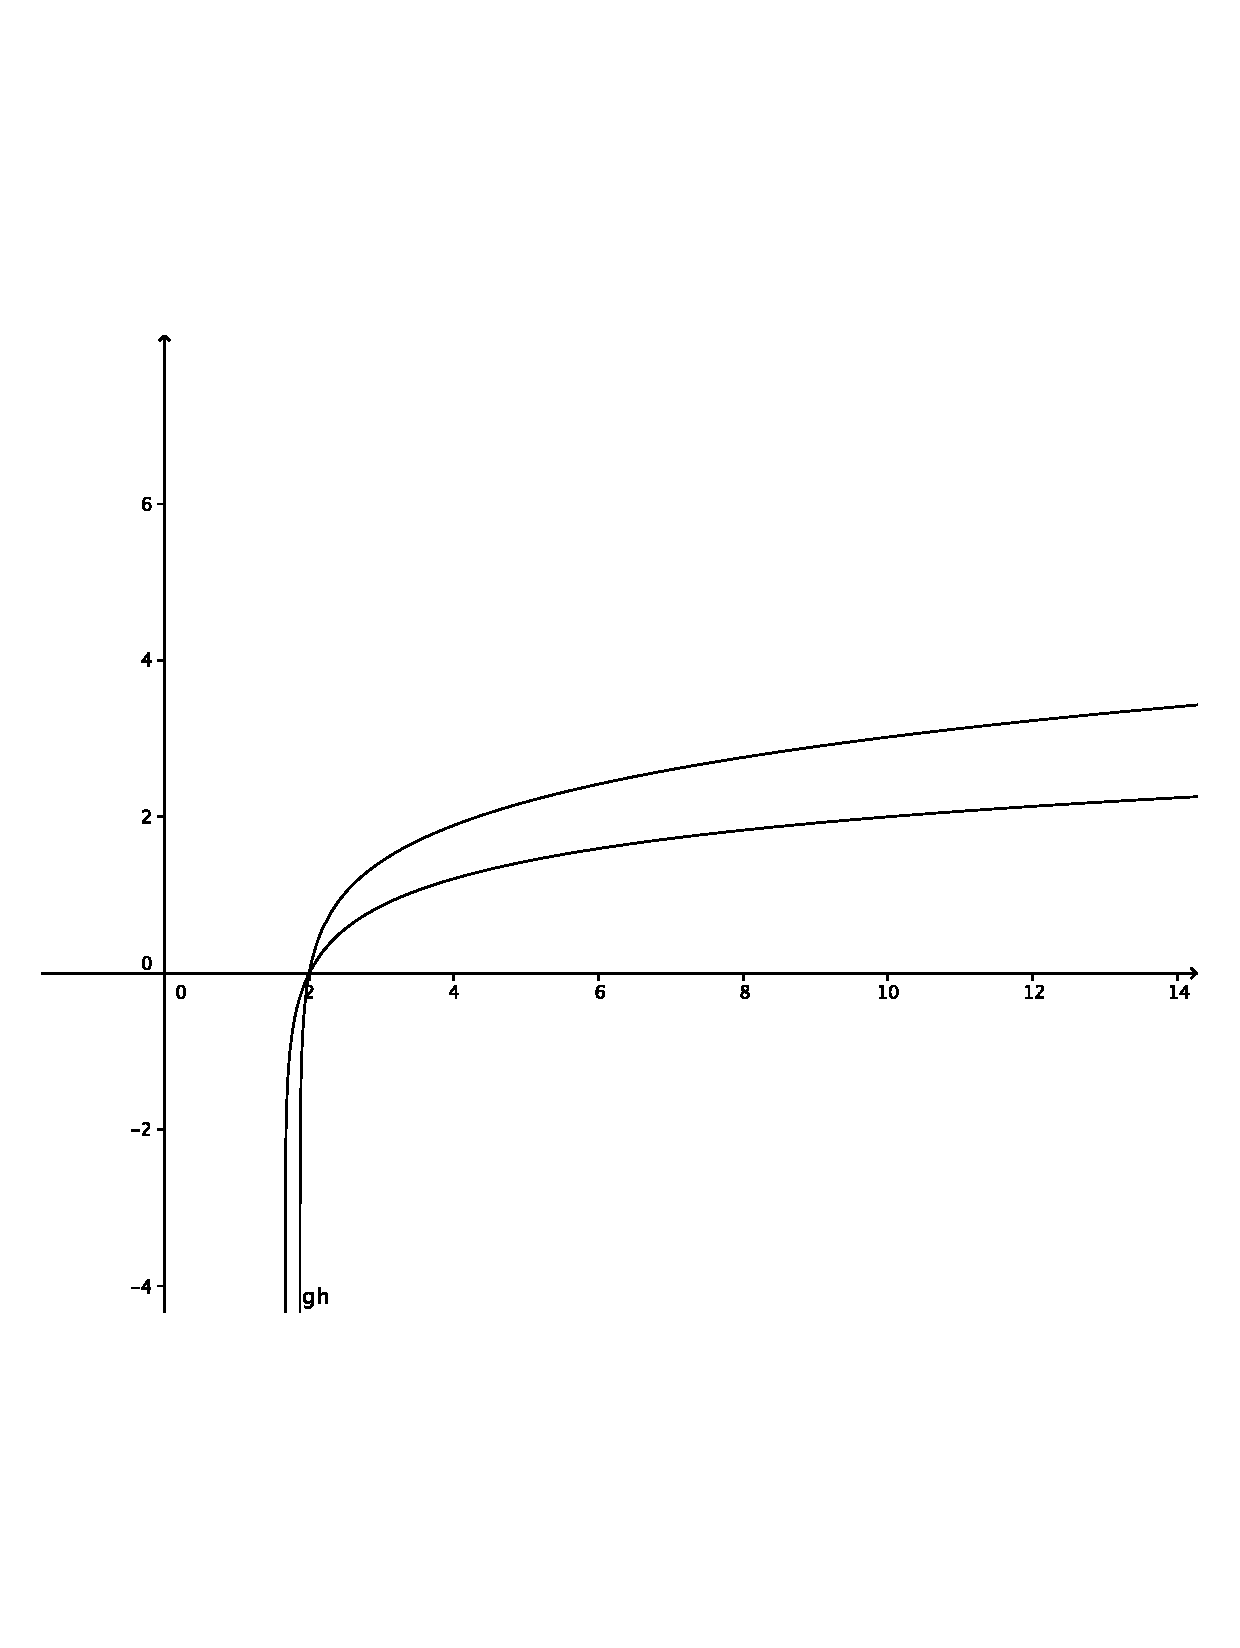
\includegraphics[width=10.7cm]{figuren/euler_expfuncties/fig_log_vgl_vb3.pdf}
%    \caption{Snijpunt van de functies $f(x)= \log_5(3x-5)$ en $g(x)=\log_5(x^2+4x-11)$}
%    \label{fig: fig_log_vgl_vb3}
%%\end{figure}

%%%%%%%%%%%%%%%%%%%%%%%%%%%%%%%%%
% Laatste aanpassing:           %
% 6 sept 2013 [Jan]: kleine aanpassingen
% 28/06/13 [Greetje]: Verbeterd en examenvragen van Leentje toegevoegd
% 23/3/11 [Greetje]: Volledig herwerkt
%
% 10/09/01 door Greetje
%   verbeteringen van Roos
%   rekenregels weggelaten
%
% 01/09/01 door Greetje          %
%%%%%%%%%%%%%%%%%%%%%%%%%%%%%%%%%

\section{Oefeningen}
\begin{oef}     
Los de volgende vergelijkingen op naar $x$. 
\begin{multicols}{2}
\begin{enumerate}
  \item $3^{-x+2}=0,7^{2\cdot x}$
  \item $4^{x}-5\cdot 2^{x}-24=0$
  \item $3^{x}+3^{x+1}=4$
  \item $3^{x+1}-26=3\cdot 3^{-x}$
  \item $2^{3^x}=8$
  \item $9^{x+1}-2\cdot 3^{x+2}-27=0$
  \item $5^{x+1}=5^{3x+1}$
  \item $2^{x+3}=16^{x-3}$
  \item $3^x=59049$
  \item $\left(\frac12\right)^x=2048$
  \item $7^x=2\cdot 8^x$
  \item $2^{x+3}=16^{x-3}$
  \item $100 \cdot 1,05^x=2000\cdot 1,025^x$
  \item $15\cdot 3^{x+1}-243\cdot 5^{x-2}=0$
  \item $3^{4x+5}=5^{x-1}$
  \item $512 + 2^{2x} = 2^{4+x}+2^{5+x}$
\end{enumerate}
\end{multicols}
\begin{opl}
\begin{enumerate}
  \item \[
          \begin{array}{rrclcl}
                 & 3^{-x+2} & = & 0.7^{2x} \\
            \iff & 9 \cdot 3^-x & = & 0.7^{2x} \\
            \iff & 9 & = & 0.7^{2x} \cdot 3^x \\
            \iff & 9 & = & (0.7^2 \cdot 3)^x \\
            \iff & \log(9) & = & x \log(0.7^2 \cdot 3) \\
            \iff & x & = & \frac{\log(9)}{\log(0.7^2 \cdot 3)} & \approx & 5.70319
          \end{array}
        \]
  \item \[
          \begin{array}{rrclcl}
                 & 4^x - 5 \cdot 2^x - 24 = 0
            \iff & (2^x)^2 - 5 \cdot 2^x - 24 = 0
          \end{array}
        \]
        We voeren $z = 2^x$ in, dit geeft ons
        \[
          z^2 - 5z - 24 = 0
        \]
        Dit is een vierkantsvergelijking met als discriminant
        \[
          D = (-5)^2 - 4 \cdot 1 \cdot (-24) = 25 + 4 \cdot 24 = 121
        \]
        en met twee oplossingen
        \[
          z_1 = \frac{5 - \sqrt{D}}{2} = -3 \qquad z_2 = \frac{5+\sqrt{D}}{2} = 8
        \]
        Dit geeft ons
        \[
          2^{x_1} = -3 \qquad 2^{x_2} = 8
        \]
        De linkervergelijking heeft geen oplossing, de rechter heeft als oplossing $x_2 = \log_2(8) = 3$.
  \item \[
          \begin{array}{rrclcl}
                 & 3^x+3^{x+1} & = & 4 \\
            \iff & 3^x+3^x\cdot3 & = & 4 \\
            \iff & 3^x(1+3) & = & 4 \\
            \iff & 3^x & = & 1 \\
            \iff & x & = & 0
          \end{array}
        \]
  \item \[
          \begin{array}{rrclcl}
                 & 3^{x+1}-26 & = & 3 \cdot 3^{-x} \\
            \iff & 3^{2x+1}-26 \cdot 3^x & = & 3 \\
            \iff & 3 \cdot (3^x)^2-26 \cdot 3^x - 3 & = & 0 \\
          \end{array}
        \]
        Substitutie $z = 3^x$
        \[
          3 z^2 - 26 z - 3 = 0
        \]
        Dit is een vierkantsvergelijking met
        \[
          D = (-26)^2 - 4 \cdot 3 \cdot (-3) = 712
        \]
        en
        \[
          z_1 = \frac{26 - \sqrt{D}}{6} \approx -0.11 \qquad z_2 = \frac{26 + \sqrt{D}}{6} \approx 8.78
        \]
        $z_1 = 3^x$ geeft ons geen oplossingen, maar
        \[
          \frac{26 + \sqrt{D}}{6} = 3^x \iff x = \log_3\left( \frac{26 + \sqrt{712}}{6} \right) \approx 1.98
        \]
  \item \[
          \begin{array}{rrclcl}
                 & 2^{(3^x)} & = & 8 \\
            \iff & 2^{(3^x)} & = & 2^3 \\
            \iff & 3^x & = & 3 \\
            \iff & x & = & 1
          \end{array}
        \]
  \item \[
          \begin{array}{rrclcl}
                 & 9^{x+1}-2 \cdot 3^{x+2}-27 & = & 0 \\
            \iff & 9 \cdot (3^x)^2 - 18 \cdot 3^x - 27 & = & 0
          \end{array}
        \]
        Substitutie $z = 3^x$
        \[
          9 z^2 - 18 z - 27 = 0
        \]
        Dit geeft een vierkantsvergelijking met
        \[
          D = (-18)^2 - 4 \cdot 9 \cdot (-27) = 1296 \qquad \sqrt{D} = 36
        \]
        en oplossingen
        \[
          z_1 = \frac{18 - 36}{18} = -1 \qquad z_2 = \frac{18 + 36}{18} = 3
        \]
        $z_1 = -1$ geeft geen oplossingen voor $x$, maar
        \[
          3 = 3^x \iff x = 1
        \]
  \item \[
          \begin{array}{rrclcl}
                 & 5^{x+1} & = & 5^{3x+1} \\
            \iff & 5^x & = & 5^{3x} \\
            \iff & x & = & 3x \\
            \iff & x & = & 0
          \end{array}
        \]
  \item \[
          \begin{array}{rrclcl}
                 & 2^{x+3} & = & 16^{x-3} \\
            \iff & 2^x \cdot 2^3 & = & 2^{3x} \cdot 2^{-9} \\
            \iff & 2^{10} & = & 2^{2x} \\
            \iff & 10 & = & 2x \\
            \iff & x & = & 5
          \end{array}
        \]
  \item $3^x=59049 \iff x = \log_3(59049) = 10$
  \item \[
          \begin{array}{rrclcl}
                 & \displaystyle \left(\frac12\right)^x & = & 2048 \\[2mm]
            \iff & 2^{-x} & = & 2^{11} \\
            \iff & x & = & -11
          \end{array}
        \]
  \item \[
          \begin{array}{rrclcl}
                 & 7^x & = & 2 \cdot 8^x \\[2mm]
            \iff & \displaystyle\left(\frac78\right)^x & = & 2 \\[2mm]
            \iff & \displaystyle x \cdot \log(\frac78) & = & \log(2) \\[2mm]
            \iff & x & = & \displaystyle \frac{\log(2)}{\log(7) - 3 \log(2)}
          \end{array}
        \]
  \item \[
          \begin{array}{rrclcl}
                 & 2^{x+3} & = & 16^{x-3} \\
            \iff & 2^x \cdot 2^3 & = & 2^{4x} \cdot 2^{-12} \\
            \iff & 2^{15} & = & 2^{3x} \\
            \iff & x & = & 5
          \end{array}
        \]
  \item \[
          \begin{array}{rrclcl}
                 & 100 \cdot 1,05^x & = & 2000\cdot 1,025^x \\[2mm]
            \iff & \displaystyle\left(\frac{1.05}{1.025}\right)^x & = & 20 \\[2mm]
            \iff & x & = & \displaystyle \frac{\log(20)}{\log(1.05)-\log(1.025)} & \approx & 124.3
          \end{array}
        \]
  \item \[
          \begin{array}{rrclcl}
                 & 15 \cdot 3^{x+1}-243 \cdot 5^{x-2} & = & 0 \\ 
            \iff & 15 \cdot 3^x \cdot 3 & = & 243 \cdot 5^x \cdot 25^{-1} \\[2mm]
            \iff & 3^x \cdot 5^{-x} & = & \displaystyle \frac{243}{15 \cdot 3 \cdot 25} \\[2mm]
            \iff & \displaystyle \left(\frac{3}{5}\right)^x & = & \displaystyle \frac{27}{125} \\[2mm]
            \iff & \displaystyle x \cdot \log\left(\frac{3}{5}\right) & = & \displaystyle \log\left(\frac{27}{125}\right) \\[2mm]
            \iff & \displaystyle x \cdot \log\left(\frac{3}{5}\right) & = & \displaystyle \log\left(\frac{3^3}{5^3}\right) \\[2mm]
            \iff & \displaystyle x \cdot \log\left(\frac{3}{5}\right) & = & \displaystyle 3 \cdot \log\left(\frac{3}{5}\right) \\[2mm]
            \iff & x & = & 3 
          \end{array}
        \]
  \item \[
          \begin{array}{rrclcl}
                 & 3^{4x+5} & = & 5^{x-1} \\
            \iff & 3^{4x} \cdot 3^5 & = & 5^{x} \cdot 5^{-1} \\[2mm]
            \iff & \left(3^4 \cdot 5^{-1}\right)^x & = & 5^{-1} \cdot 3^{-5} \\[2mm]
            \iff & x \cdot \log\left(3^4 \cdot 5^{-1}\right) & = & \log(5^{-1} \cdot 3^{-5}) \\[2mm]
            \iff & x & = & \displaystyle \frac{\log(5^{-1} \cdot 3^{-5})}{\log\left(3^4 \cdot 5^{-1}\right)} \\[3mm]
            \iff & x & = & \displaystyle \frac{-\log(5) - 5 \log(3)}{4\log(3) - \log(5)} & \approx & -2.55
          \end{array}
        \]
  \item \[
          \begin{array}{rrclcl}
                 & 512 + 2^{2x} & = & 2^{4+x}+2^{5+x} \\
            \iff & 2^9 + (2^x)^2 & = & (2^4 + 2^5) \cdot 2^x \\
            \iff & (2^x)^2 - (2^4 + 2^5) \cdot 2^x + 2^9 & = & 0 \\
            \iff & (2^x)^2 - 48 \cdot 2^x + 512 & = & 0
          \end{array}
        \]
        Substitutie $z = 2^x$.
        \[
          z^2 - 48 z + 512 = 0
        \]
        Dit is een vierkantsvergelijking met
        \[
          D = 48^2 - 4 \cdot 1 \cdot 512 = 256 \qquad \sqrt{D} = 16
        \]
        en oplossingen
        \[
          z_1 = \frac{48 - 16}{2} = 16 \qquad z_2 = \frac{48+16}{2} = 32
        \]
        Dit geeft voor $x$
        \[
          2^{x_1} = 16 \iff x_1 = 4 \qquad 2^{x_2} = 32 \iff x_2 = 5
        \]
\end{enumerate}
\end{opl}
\end{oef}

% Oefeningen op logaritmische vergelijkingen
%\begin{oef} $\qquad$
% \\
%\begin{multicols}{2}
%\begin{enumerate}
%\item   $3 \cdot \log_{2}2 +\log_{2}x=3$ 
%\\ \item   $\log_{x}(\sqrt{3})=3$
%\\ \item    $\log(2x+3)+\log(x-1)=\log(x^{2}+9)$
%\\ \item     $\log_{64}(\log_{x}(16))^{3}=1$ 
%\\ \item $(\log_{2}x)^{3}+\log_{2}(x^{4})=4\cdot (\log_{2}x)^{2}$
%\\ \item  $\displaystyle{\log_{2}x=\frac{1}{\log_{6-x}4}}$
%\\ \item $\log_{2}(2^{x}-7)+x=3$
%\\ \item $\log_{x}(2\cdot x+8)=2$ 
%\\ \item $\log(x-3)+\log(x+1)=\log(2x+2)$
%\\ \item  $\left[\log(x+2)\right]^3+\left[\log(x+2)\right]^2=\log\left[(x+2)^2\right]$
% \end{enumerate}
%    
%\end{multicols}
%
%     \end{oef}
     
\begin{oef}
Een blad papier is 1 mm dik. We plooien dit blad een
\emph{aantal keren na elkaar} dubbel. In de veronderstelling dat
we dit proces heel dikwijls na elkaar \emph{kunnen} uitvoeren,
hoeveel keren moeten we minstens plooien opdat de dikte van
het geplooide blad papier meer dan 2 cm zou meten?
\begin{opl}
Dikte van geplooide papier: $D(t)=2^t$.\\
Zoek $t$ zodat $D(t)=20$. Dit geeft $t=\log20/\log 2=4,32$.\\
Antwoord: na vijf keer plooien is dikte meer dan 2 cm.
\end{opl}
\end{oef}

\begin{oef}
We nemen aan dat op korte termijn de waarde van een aandeel stijgt
volgens een exponentieel  proces. Op 10 maanden is de prijs van
het aandeel verdrievoudigd.
\begin{enumerate}
  \item Bepaal de groeifactor (i) per 10 maand en (ii) per maand van dit groeiproces.
  \item Als je weet dat het aandeel nu het vijfvoud is van
        toen het werd aangekocht, hoeveel maanden geleden is het dan
        aangekocht?
\end{enumerate}
\begin{opl}
  \begin{enumerate}
    \item $g_{10}=3$; $g_m=3^\frac{1}{10}$
    \item Waarde van aandeel in functie van de tijd: $B(t)=B(0)\cdot 3^\frac{t}{10}$ \\
          Zoek $t$ zodat $B(t)=5B(0)$. Dat geeft $t=\log5/\log3^\frac{1}{10}=14,65$, dus na 14,65 maanden.
  \end{enumerate}
\end{opl}
\end{oef}

 
\begin{figure}[hbtp]
  \flushright
  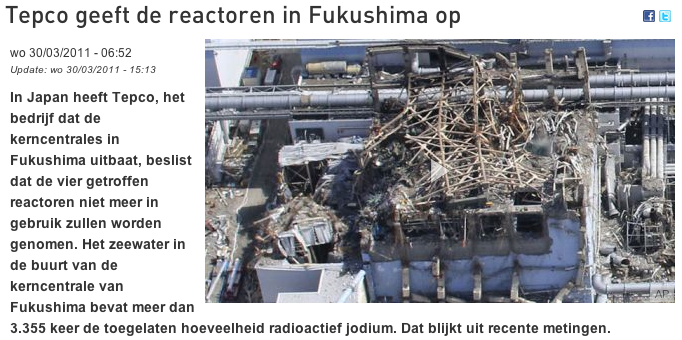
\includegraphics[width=0.95\textwidth]{oefeningen/jodiumderedactie.png}
  \caption{Fukushima -- De redactie, 30 maart 2011}
  \label{fig:fukushima} 
\end{figure}    

\begin{oef}
In 2011 werd Japan getroffen door een zware aardbeving met bijbehorende tsunami. De kernreactoren in Fukushima konden niet meer gekoeld worden en ontploften gedeeltelijk. Op 30 maart 2011 (figuur~\ref{fig:fukushima}) bleek de hoeveelheid radioactief Jodium in het zeewater ($\text{I}^{131}$) 3355 keer de toegelaten hoeveelheid te bedragen. 
De Japanse overheid beweerde dat er geen probleem was voor de consumptie van vis uit de zee, want de radioactiviteit zou snel verdund worden. Bereken hoelang het duurt (bij deze verontreiniging) tot de radioactiviteit van het $\text{I}^{131}$ terug gelijk is aan de toegelaten hoeveelheid. De halveringstijd van $\text{I}^{131}$ is 8 dagen.
\begin{opl}
$J(t)=3355\cdot J_0\cdot \left( \frac12\right)^\frac{t}{8}$\\
Zoek $t$ zodat $J(t)=J_0$\\
$t=8\frac{\log \frac{1}{3355}}{\log\frac12}=93,70$, dus na 93,70 dagen.
\end{opl}
\end{oef}


\begin{oef}
Op een archeologische site werden muurschilderingen
teruggevonden. De ouderdom van de schildering wordt bepaald
met de $\text{C}^{14}$-proef.  Men weet immers  dat de
hoeveelheid van dit isotoop jaarlijks exponentieel daalt met factor
\num{0.99988}. Op de schilderingen werd \SI{20}{\percent} van de
oorspronkelijke hoeveelheid $\text{C}^{14}$ teruggevonden. Hoe oud
zijn de schilderingen?
\begin{opl}
  $C(t)=0,20\cdot C_0\cdot 0,9988^t$\\
  Zoek $t$ zodat $C(t)=C_0$\\
  $t=\frac{\log5}{\log0,9988}=-13411$, dus 13411 jaar geleden.
\end{opl}
\end{oef}

\begin{oef}
  Jan zet \euros{1900} op een spaarboekje tegen samengestelde
      intrest van \SI{5}{\percent} per jaar en \euros{1000} op een andere rekening,
      waarvan de verdubbelingstijd van het kapitaal 25 jaar bedraagt.
      Wanneer zal het bedrag op het spaarboekje dubbel zo
      groot zijn als het bedrag op de rekening?
\begin{opl}
Groeifunctie van spaarboekje 1: $S_1(t)=1900\cdot 1,05^t$; \\Groeifunctie van spaarboekje 2: $S_2(t)=1000\cdot 2^\frac{t}{25}$\\
Zoek $t$ zodat $S_1(t)=2\cdot S_2(t)$, wat geeft $t=\frac{\log(19/20)}{\log(2^{1/25}/1,05)}=2,435$.\\
Antwoord: na 2,435 jaar is het bedrag van het spaarboekje dubbel zo groot als het bedrag op de rekening.
\end{opl}
\end{oef}



\begin{oef}
  De waarde van een schilderij van Rembrandt neemt per
      decennium (periode van 10 jaar) toe met \SI{20}{\percent}. De waarde van een schilderij
      van Picasso stijgt in waarde met \SI{5}{\percent}  per jaar. Een
      kunsthandelaar koopt vandaag een schilderij van Rembrandt voor
      \euros{300\,000} en een schilderij van Picasso voor
      \euros{225\,000}.
      Wanneer zullen beide schilderijen evenveel waard zijn?
      \begin{opl}
         De waarde van de Rembrandt: $R(t)=300000\cdot 1,20^{t/10}$\\
         De waarde van de Picasso: $P(t)=225000\cdot 1,05^t$\\
         Zoek $t$ zodat $P(t)=R(t)$, wat geeft $t=\log(300/225)/\log(1,05/1,20^{1/10})=9,41$.\\
         Antwoord: na 9,41 jaar zijn beide schilderijen evenveel waard.
      \end{opl}
\end{oef}

\begin{oef}
 Land A heeft 80 miljoen inwoners en land B heeft er 100
      miljoen. De bevolking van land A verdubbelt in 20 jaar en die
      van land B groeit elk jaar aan met \SI{2,3}{\percent}.
      \begin{enumerate}
          \item  Bereken de groeifactor per jaar van land A.
      \item Bereken de verdubbelingstijd voor land B.
          \item Wanneer zal het aantal inwoners van land A gelijk zijn
            aan dat van land B?
      \end{enumerate}
      \begin{opl}
	$A(t)=80\cdot 2^{t/20}$; $B(t)=100\cdot 1,023^t$;\\
	Zoek $t$ zodat $A(t)=B(t)$, wat geeft $t=\log(8/10)/\log(1,023/2^{1/20})=18,72$\\
	Antwoord: na 18,72 jaar zal het aantal inwoners gelijk zijn.
      \end{opl}
\end{oef}

\begin{oef}
Wim is nu 7 jaar oud en wil op zijn twaalfde
verjaardag een
fiets met 10 versnellingen als geschenk. Zijn ouders willen nu
reeds een bedrag op een spaarrekening zetten van \euros{400} tegen een
jaarlijkse rente van \SI{7}{\percent}.
\begin{enumerate}
  \item Over welk bedrag beschikt Wim op zijn twaalfde verjaardag?
  \item Wanneer zal het bedrag op Wim's spaarrekening verdubbeld zijn?
\end{enumerate}
\begin{opl}
  Groeifunctie die het gespaarde bedrag $t$ jaar na de zevende verjaardag weergeeft: $B(t)=400\cdot 1,07^t$\\
  \begin{enumerate}
    \item bedrag op rekening bij twaalfde verjaardag: $B(5)=561,02$
    \item Zoek $t$ zodat $B(t)=800$, wat geeft $t=\log2/\log1,07=10,24$, dus als Wim 17,24 jaar is, heeft hij 800\euros op zijn rekening staan.
  \end{enumerate}
\end{opl}
\end{oef}



\begin{oef}
Een vader wil nu een bedrag van \euros{10\,000} verdelen over zijn
2 kinderen van respectievelijk 10 en \num{14,5} jaar oud. De vader wil
dat de verdeling zo verloopt, dat elk kind later op zijn
\'{e}\'{e}nentwintigste verjaardag \emph{hetzelfde} kapitaal ontvangt.
De jaarlijkse rente op beide rekeningen is dezelfde en bedraagt \SI{7}{\percent}.
\begin{enumerate}
  \item Welk bedrag wordt nu voor elk kind belegd?
  \item Over welk bedrag zal ieder kind beschikken op zijn
        \'e\'enentwintigste verjaardag?
\end{enumerate}
\begin{opl}
Bedrag op rekening van kind 1: $B_1(t)=B_1\cdot 1,07^t$ met $t$ het aantal jaren sinds `nu'.\\
Bedrag op rekening van kind 2: $B_2(t)=B_2\cdot 1,07^t$ met $B_1+B_2=\num{10000}$; \\
Zoek $B_1$ en $B_2$ zodat $B_1(11)=B_2(6,5)$. Omdat $B_1+B_2=\num{10000}$, moeten we $B_1$ zoeken zodat 
$B_1\cdot 1,07^{11}=(10000-B_1)\cdot 1,07^{6,5}$, wat geeft $B_1=4244$. \\
Antwoord: Nu wordt \euros{4244} en \euros{5755} belegd.\\
Op zijn  \'{e}\'{e}nentwintigste verjaardag zal het kind beschikken over \euros{8934}.
\end{opl}
\end{oef}




\begin{oef}
Een kapitaal van \euros{3000} wordt uitgezet tegen samengestelde intrest
en groeit aan tot \euros{\num{4432.37}} na 8 jaar. Na hoeveel tijd is dit bedrag \euros{5000} geworden?
\begin{opl}
Eerst zoeken we de groeifactor uit de vergelijking:\\
$3000\cdot g^{8} = 4432,37$\\
Hieruit vinden we dat $g$ gelijk is aan $1,05$. Het kapitaal groeit dus met \SI{5}{\percent} per jaar.\\
Nu kunnen we berekenen wanneer het kapitaal aangegroeid is tot \euros{5000}\\
$3000\cdot 1,05^{t} = 5000$\\
$t = \log(5/3)/\log(1,05)$\\
$t = 10,46$\\
Hieruit vinden we dat het kapitaal $11$ jaar op de bank moet blijven staan vooraleer het is aangegroeid tot \euros{5000}.
\end{opl}
\end{oef}
  

% Opm. Inge: oefening is wat verwarrend, doders doen in het begin niets? Vreemd. Beter weglaten   
%\begin{oef}
%   Het is nat en koud en je hebt een stevige bronchitis te pakken. De dokter laat bloed nemen en stelt vast dat je \SI{40500} bacteriën in je bloed hebt, die zich ieder etmaal (=\SI{24}{\hour)} verdubbelen in aantal. Je zit midden in de examenperiode en wilt zo snel mogelijk van die kleine ettertjes verlost worden. De dokter injecteert je met een hoge concentratie bacterie-doders. Na de injectie heb je 3000 bacterie-doders in je bloed, die zich iedere \SI{8}{\hour} verdubbelen. Je zult je stukken beter voelen zodra het aantal bacterie-doders groter wordt dan het aantal bacteriën. Na hoeveel uur zal je van je bronchitis verlost zijn? 
%   \begin{enumerate}
%\item Bereken zowel  voor de kolonie bacteriën als voor de bacterie-doders de groeifactor per uur.
%
%\item Stel de vergelijkingen op die hun groei simuleren.
%
%\item Reken uit na hoeveel uur hun aantallen gelijk worden en je de strijdt tegen je bronchitis wint.
%
%   \end{enumerate}
%   \begin{opl}
%   $B(t)=40500\cdot 2^{t/24}$; $D(t)=3000\cdot 2^{t/8}$. Na \SI{5,2} uur zijn er meer bacterie-doders dan bacteriën.
%   \end{opl}
%   \end{oef}


\begin{oef}
Het wordt steeds duidelijker dat de mensen wegtrekken uit de grote steden in Belgi\"e. Brussel had in 2010 nog \num{1124000} inwoners, en ziet zijn inwonertal dalen met \SI{10}{\percent} per decennium (= 10 jaar). Leuven en omstreken blijken echter zeer gegeerd. Met een inwonertal van \num{95500} in 2010 was Groot-Leuven nog een kleine stad. Het lijkt er echter op dat dit inwonertal zal verdubbelen per 8 jaar. Hoe lang duurt het vooraleer Leuven en Brussel even groot geworden zijn?
\begin{enumerate}
\item Bereken voor het aantal inwoners van Brussel en Leuven de jaarlijkse groeifactor.
\item	Stel de vergelijkingen op die de groei/daling van de bevolking in Brussel en Leuven simuleren.
\item Reken uit na hoeveel jaar Leuven evenveel inwoners telt als Brussel.
\end{enumerate}
\begin{opl}
$B(t)=\num{1124000}\cdot 0,9^{t/10}$ en $L(t)=\num{95500}\cdot 2^{t/8}$ met $t$ uitgedrukt in jaren. Na \SI{25,37} jaren telt Leuven evenveel inwoners als Brussel. 
\end{opl}
\end{oef}


%%% Local Variables: 
%%% mode: latex
%%% TeX-master: "../cursusTW1"
%%% End: 


%%% Local Variables: 
%%% mode: latex
%%% TeX-master: "cursusTW1"
%%% End: 

\newpage 
%%%%%%%%%%%%%%%%%%%%%%%%%%%%%%%%%
% Laatste aanpassing:           %
% 6 sept 2013 [Jan]: kleine aanpassingen
% 28/06/13 [Greetje]: Verbeterd en examenvragen van Leentje toegevoegd
% 23/3/11 [Greetje]: Volledig herwerkt
%
% 10/09/01 door Greetje
%   verbeteringen van Roos
%   rekenregels weggelaten
%
% 01/09/01 door Greetje          %
%%%%%%%%%%%%%%%%%%%%%%%%%%%%%%%%%

\section{Oefeningen}
\begin{oef}     
Los de volgende vergelijkingen op naar $x$. 
\begin{multicols}{2}
\begin{enumerate}
  \item $3^{-x+2}=0,7^{2\cdot x}$
  \item $4^{x}-5\cdot 2^{x}-24=0$
  \item $3^{x}+3^{x+1}=4$
  \item $3^{x+1}-26=3\cdot 3^{-x}$
  \item $2^{3^x}=8$
  \item $9^{x+1}-2\cdot 3^{x+2}-27=0$
  \item $5^{x+1}=5^{3x+1}$
  \item $2^{x+3}=16^{x-3}$
  \item $3^x=59049$
  \item $\left(\frac12\right)^x=2048$
  \item $7^x=2\cdot 8^x$
  \item $2^{x+3}=16^{x-3}$
  \item $100 \cdot 1,05^x=2000\cdot 1,025^x$
  \item $15\cdot 3^{x+1}-243\cdot 5^{x-2}=0$
  \item $3^{4x+5}=5^{x-1}$
  \item $512 + 2^{2x} = 2^{4+x}+2^{5+x}$
\end{enumerate}
\end{multicols}
\begin{opl}
\begin{enumerate}
  \item \[
          \begin{array}{rrclcl}
                 & 3^{-x+2} & = & 0.7^{2x} \\
            \iff & 9 \cdot 3^-x & = & 0.7^{2x} \\
            \iff & 9 & = & 0.7^{2x} \cdot 3^x \\
            \iff & 9 & = & (0.7^2 \cdot 3)^x \\
            \iff & \log(9) & = & x \log(0.7^2 \cdot 3) \\
            \iff & x & = & \frac{\log(9)}{\log(0.7^2 \cdot 3)} & \approx & 5.70319
          \end{array}
        \]
  \item \[
          \begin{array}{rrclcl}
                 & 4^x - 5 \cdot 2^x - 24 = 0
            \iff & (2^x)^2 - 5 \cdot 2^x - 24 = 0
          \end{array}
        \]
        We voeren $z = 2^x$ in, dit geeft ons
        \[
          z^2 - 5z - 24 = 0
        \]
        Dit is een vierkantsvergelijking met als discriminant
        \[
          D = (-5)^2 - 4 \cdot 1 \cdot (-24) = 25 + 4 \cdot 24 = 121
        \]
        en met twee oplossingen
        \[
          z_1 = \frac{5 - \sqrt{D}}{2} = -3 \qquad z_2 = \frac{5+\sqrt{D}}{2} = 8
        \]
        Dit geeft ons
        \[
          2^{x_1} = -3 \qquad 2^{x_2} = 8
        \]
        De linkervergelijking heeft geen oplossing, de rechter heeft als oplossing $x_2 = \log_2(8) = 3$.
  \item \[
          \begin{array}{rrclcl}
                 & 3^x+3^{x+1} & = & 4 \\
            \iff & 3^x+3^x\cdot3 & = & 4 \\
            \iff & 3^x(1+3) & = & 4 \\
            \iff & 3^x & = & 1 \\
            \iff & x & = & 0
          \end{array}
        \]
  \item \[
          \begin{array}{rrclcl}
                 & 3^{x+1}-26 & = & 3 \cdot 3^{-x} \\
            \iff & 3^{2x+1}-26 \cdot 3^x & = & 3 \\
            \iff & 3 \cdot (3^x)^2-26 \cdot 3^x - 3 & = & 0 \\
          \end{array}
        \]
        Substitutie $z = 3^x$
        \[
          3 z^2 - 26 z - 3 = 0
        \]
        Dit is een vierkantsvergelijking met
        \[
          D = (-26)^2 - 4 \cdot 3 \cdot (-3) = 712
        \]
        en
        \[
          z_1 = \frac{26 - \sqrt{D}}{6} \approx -0.11 \qquad z_2 = \frac{26 + \sqrt{D}}{6} \approx 8.78
        \]
        $z_1 = 3^x$ geeft ons geen oplossingen, maar
        \[
          \frac{26 + \sqrt{D}}{6} = 3^x \iff x = \log_3\left( \frac{26 + \sqrt{712}}{6} \right) \approx 1.98
        \]
  \item \[
          \begin{array}{rrclcl}
                 & 2^{(3^x)} & = & 8 \\
            \iff & 2^{(3^x)} & = & 2^3 \\
            \iff & 3^x & = & 3 \\
            \iff & x & = & 1
          \end{array}
        \]
  \item \[
          \begin{array}{rrclcl}
                 & 9^{x+1}-2 \cdot 3^{x+2}-27 & = & 0 \\
            \iff & 9 \cdot (3^x)^2 - 18 \cdot 3^x - 27 & = & 0
          \end{array}
        \]
        Substitutie $z = 3^x$
        \[
          9 z^2 - 18 z - 27 = 0
        \]
        Dit geeft een vierkantsvergelijking met
        \[
          D = (-18)^2 - 4 \cdot 9 \cdot (-27) = 1296 \qquad \sqrt{D} = 36
        \]
        en oplossingen
        \[
          z_1 = \frac{18 - 36}{18} = -1 \qquad z_2 = \frac{18 + 36}{18} = 3
        \]
        $z_1 = -1$ geeft geen oplossingen voor $x$, maar
        \[
          3 = 3^x \iff x = 1
        \]
  \item \[
          \begin{array}{rrclcl}
                 & 5^{x+1} & = & 5^{3x+1} \\
            \iff & 5^x & = & 5^{3x} \\
            \iff & x & = & 3x \\
            \iff & x & = & 0
          \end{array}
        \]
  \item \[
          \begin{array}{rrclcl}
                 & 2^{x+3} & = & 16^{x-3} \\
            \iff & 2^x \cdot 2^3 & = & 2^{3x} \cdot 2^{-9} \\
            \iff & 2^{10} & = & 2^{2x} \\
            \iff & 10 & = & 2x \\
            \iff & x & = & 5
          \end{array}
        \]
  \item $3^x=59049 \iff x = \log_3(59049) = 10$
  \item \[
          \begin{array}{rrclcl}
                 & \displaystyle \left(\frac12\right)^x & = & 2048 \\[2mm]
            \iff & 2^{-x} & = & 2^{11} \\
            \iff & x & = & -11
          \end{array}
        \]
  \item \[
          \begin{array}{rrclcl}
                 & 7^x & = & 2 \cdot 8^x \\[2mm]
            \iff & \displaystyle\left(\frac78\right)^x & = & 2 \\[2mm]
            \iff & \displaystyle x \cdot \log(\frac78) & = & \log(2) \\[2mm]
            \iff & x & = & \displaystyle \frac{\log(2)}{\log(7) - 3 \log(2)}
          \end{array}
        \]
  \item \[
          \begin{array}{rrclcl}
                 & 2^{x+3} & = & 16^{x-3} \\
            \iff & 2^x \cdot 2^3 & = & 2^{4x} \cdot 2^{-12} \\
            \iff & 2^{15} & = & 2^{3x} \\
            \iff & x & = & 5
          \end{array}
        \]
  \item \[
          \begin{array}{rrclcl}
                 & 100 \cdot 1,05^x & = & 2000\cdot 1,025^x \\[2mm]
            \iff & \displaystyle\left(\frac{1.05}{1.025}\right)^x & = & 20 \\[2mm]
            \iff & x & = & \displaystyle \frac{\log(20)}{\log(1.05)-\log(1.025)} & \approx & 124.3
          \end{array}
        \]
  \item \[
          \begin{array}{rrclcl}
                 & 15 \cdot 3^{x+1}-243 \cdot 5^{x-2} & = & 0 \\ 
            \iff & 15 \cdot 3^x \cdot 3 & = & 243 \cdot 5^x \cdot 25^{-1} \\[2mm]
            \iff & 3^x \cdot 5^{-x} & = & \displaystyle \frac{243}{15 \cdot 3 \cdot 25} \\[2mm]
            \iff & \displaystyle \left(\frac{3}{5}\right)^x & = & \displaystyle \frac{27}{125} \\[2mm]
            \iff & \displaystyle x \cdot \log\left(\frac{3}{5}\right) & = & \displaystyle \log\left(\frac{27}{125}\right) \\[2mm]
            \iff & \displaystyle x \cdot \log\left(\frac{3}{5}\right) & = & \displaystyle \log\left(\frac{3^3}{5^3}\right) \\[2mm]
            \iff & \displaystyle x \cdot \log\left(\frac{3}{5}\right) & = & \displaystyle 3 \cdot \log\left(\frac{3}{5}\right) \\[2mm]
            \iff & x & = & 3 
          \end{array}
        \]
  \item \[
          \begin{array}{rrclcl}
                 & 3^{4x+5} & = & 5^{x-1} \\
            \iff & 3^{4x} \cdot 3^5 & = & 5^{x} \cdot 5^{-1} \\[2mm]
            \iff & \left(3^4 \cdot 5^{-1}\right)^x & = & 5^{-1} \cdot 3^{-5} \\[2mm]
            \iff & x \cdot \log\left(3^4 \cdot 5^{-1}\right) & = & \log(5^{-1} \cdot 3^{-5}) \\[2mm]
            \iff & x & = & \displaystyle \frac{\log(5^{-1} \cdot 3^{-5})}{\log\left(3^4 \cdot 5^{-1}\right)} \\[3mm]
            \iff & x & = & \displaystyle \frac{-\log(5) - 5 \log(3)}{4\log(3) - \log(5)} & \approx & -2.55
          \end{array}
        \]
  \item \[
          \begin{array}{rrclcl}
                 & 512 + 2^{2x} & = & 2^{4+x}+2^{5+x} \\
            \iff & 2^9 + (2^x)^2 & = & (2^4 + 2^5) \cdot 2^x \\
            \iff & (2^x)^2 - (2^4 + 2^5) \cdot 2^x + 2^9 & = & 0 \\
            \iff & (2^x)^2 - 48 \cdot 2^x + 512 & = & 0
          \end{array}
        \]
        Substitutie $z = 2^x$.
        \[
          z^2 - 48 z + 512 = 0
        \]
        Dit is een vierkantsvergelijking met
        \[
          D = 48^2 - 4 \cdot 1 \cdot 512 = 256 \qquad \sqrt{D} = 16
        \]
        en oplossingen
        \[
          z_1 = \frac{48 - 16}{2} = 16 \qquad z_2 = \frac{48+16}{2} = 32
        \]
        Dit geeft voor $x$
        \[
          2^{x_1} = 16 \iff x_1 = 4 \qquad 2^{x_2} = 32 \iff x_2 = 5
        \]
\end{enumerate}
\end{opl}
\end{oef}

% Oefeningen op logaritmische vergelijkingen
%\begin{oef} $\qquad$
% \\
%\begin{multicols}{2}
%\begin{enumerate}
%\item   $3 \cdot \log_{2}2 +\log_{2}x=3$ 
%\\ \item   $\log_{x}(\sqrt{3})=3$
%\\ \item    $\log(2x+3)+\log(x-1)=\log(x^{2}+9)$
%\\ \item     $\log_{64}(\log_{x}(16))^{3}=1$ 
%\\ \item $(\log_{2}x)^{3}+\log_{2}(x^{4})=4\cdot (\log_{2}x)^{2}$
%\\ \item  $\displaystyle{\log_{2}x=\frac{1}{\log_{6-x}4}}$
%\\ \item $\log_{2}(2^{x}-7)+x=3$
%\\ \item $\log_{x}(2\cdot x+8)=2$ 
%\\ \item $\log(x-3)+\log(x+1)=\log(2x+2)$
%\\ \item  $\left[\log(x+2)\right]^3+\left[\log(x+2)\right]^2=\log\left[(x+2)^2\right]$
% \end{enumerate}
%    
%\end{multicols}
%
%     \end{oef}
     
\begin{oef}
Een blad papier is 1 mm dik. We plooien dit blad een
\emph{aantal keren na elkaar} dubbel. In de veronderstelling dat
we dit proces heel dikwijls na elkaar \emph{kunnen} uitvoeren,
hoeveel keren moeten we minstens plooien opdat de dikte van
het geplooide blad papier meer dan 2 cm zou meten?
\begin{opl}
Dikte van geplooide papier: $D(t)=2^t$.\\
Zoek $t$ zodat $D(t)=20$. Dit geeft $t=\log20/\log 2=4,32$.\\
Antwoord: na vijf keer plooien is dikte meer dan 2 cm.
\end{opl}
\end{oef}

\begin{oef}
We nemen aan dat op korte termijn de waarde van een aandeel stijgt
volgens een exponentieel  proces. Op 10 maanden is de prijs van
het aandeel verdrievoudigd.
\begin{enumerate}
  \item Bepaal de groeifactor (i) per 10 maand en (ii) per maand van dit groeiproces.
  \item Als je weet dat het aandeel nu het vijfvoud is van
        toen het werd aangekocht, hoeveel maanden geleden is het dan
        aangekocht?
\end{enumerate}
\begin{opl}
  \begin{enumerate}
    \item $g_{10}=3$; $g_m=3^\frac{1}{10}$
    \item Waarde van aandeel in functie van de tijd: $B(t)=B(0)\cdot 3^\frac{t}{10}$ \\
          Zoek $t$ zodat $B(t)=5B(0)$. Dat geeft $t=\log5/\log3^\frac{1}{10}=14,65$, dus na 14,65 maanden.
  \end{enumerate}
\end{opl}
\end{oef}

 
\begin{figure}[hbtp]
  \flushright
  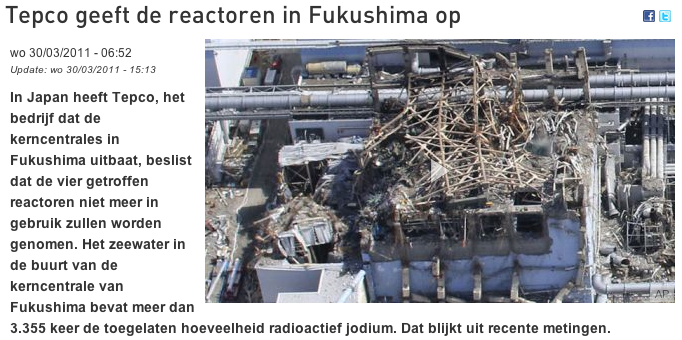
\includegraphics[width=0.95\textwidth]{oefeningen/jodiumderedactie.png}
  \caption{Fukushima -- De redactie, 30 maart 2011}
  \label{fig:fukushima} 
\end{figure}    

\begin{oef}
In 2011 werd Japan getroffen door een zware aardbeving met bijbehorende tsunami. De kernreactoren in Fukushima konden niet meer gekoeld worden en ontploften gedeeltelijk. Op 30 maart 2011 (figuur~\ref{fig:fukushima}) bleek de hoeveelheid radioactief Jodium in het zeewater ($\text{I}^{131}$) 3355 keer de toegelaten hoeveelheid te bedragen. 
De Japanse overheid beweerde dat er geen probleem was voor de consumptie van vis uit de zee, want de radioactiviteit zou snel verdund worden. Bereken hoelang het duurt (bij deze verontreiniging) tot de radioactiviteit van het $\text{I}^{131}$ terug gelijk is aan de toegelaten hoeveelheid. De halveringstijd van $\text{I}^{131}$ is 8 dagen.
\begin{opl}
$J(t)=3355\cdot J_0\cdot \left( \frac12\right)^\frac{t}{8}$\\
Zoek $t$ zodat $J(t)=J_0$\\
$t=8\frac{\log \frac{1}{3355}}{\log\frac12}=93,70$, dus na 93,70 dagen.
\end{opl}
\end{oef}


\begin{oef}
Op een archeologische site werden muurschilderingen
teruggevonden. De ouderdom van de schildering wordt bepaald
met de $\text{C}^{14}$-proef.  Men weet immers  dat de
hoeveelheid van dit isotoop jaarlijks exponentieel daalt met factor
\num{0.99988}. Op de schilderingen werd \SI{20}{\percent} van de
oorspronkelijke hoeveelheid $\text{C}^{14}$ teruggevonden. Hoe oud
zijn de schilderingen?
\begin{opl}
  $C(t)=0,20\cdot C_0\cdot 0,9988^t$\\
  Zoek $t$ zodat $C(t)=C_0$\\
  $t=\frac{\log5}{\log0,9988}=-13411$, dus 13411 jaar geleden.
\end{opl}
\end{oef}

\begin{oef}
  Jan zet \euros{1900} op een spaarboekje tegen samengestelde
      intrest van \SI{5}{\percent} per jaar en \euros{1000} op een andere rekening,
      waarvan de verdubbelingstijd van het kapitaal 25 jaar bedraagt.
      Wanneer zal het bedrag op het spaarboekje dubbel zo
      groot zijn als het bedrag op de rekening?
\begin{opl}
Groeifunctie van spaarboekje 1: $S_1(t)=1900\cdot 1,05^t$; \\Groeifunctie van spaarboekje 2: $S_2(t)=1000\cdot 2^\frac{t}{25}$\\
Zoek $t$ zodat $S_1(t)=2\cdot S_2(t)$, wat geeft $t=\frac{\log(19/20)}{\log(2^{1/25}/1,05)}=2,435$.\\
Antwoord: na 2,435 jaar is het bedrag van het spaarboekje dubbel zo groot als het bedrag op de rekening.
\end{opl}
\end{oef}



\begin{oef}
  De waarde van een schilderij van Rembrandt neemt per
      decennium (periode van 10 jaar) toe met \SI{20}{\percent}. De waarde van een schilderij
      van Picasso stijgt in waarde met \SI{5}{\percent}  per jaar. Een
      kunsthandelaar koopt vandaag een schilderij van Rembrandt voor
      \euros{300\,000} en een schilderij van Picasso voor
      \euros{225\,000}.
      Wanneer zullen beide schilderijen evenveel waard zijn?
      \begin{opl}
         De waarde van de Rembrandt: $R(t)=300000\cdot 1,20^{t/10}$\\
         De waarde van de Picasso: $P(t)=225000\cdot 1,05^t$\\
         Zoek $t$ zodat $P(t)=R(t)$, wat geeft $t=\log(300/225)/\log(1,05/1,20^{1/10})=9,41$.\\
         Antwoord: na 9,41 jaar zijn beide schilderijen evenveel waard.
      \end{opl}
\end{oef}

\begin{oef}
 Land A heeft 80 miljoen inwoners en land B heeft er 100
      miljoen. De bevolking van land A verdubbelt in 20 jaar en die
      van land B groeit elk jaar aan met \SI{2,3}{\percent}.
      \begin{enumerate}
          \item  Bereken de groeifactor per jaar van land A.
      \item Bereken de verdubbelingstijd voor land B.
          \item Wanneer zal het aantal inwoners van land A gelijk zijn
            aan dat van land B?
      \end{enumerate}
      \begin{opl}
	$A(t)=80\cdot 2^{t/20}$; $B(t)=100\cdot 1,023^t$;\\
	Zoek $t$ zodat $A(t)=B(t)$, wat geeft $t=\log(8/10)/\log(1,023/2^{1/20})=18,72$\\
	Antwoord: na 18,72 jaar zal het aantal inwoners gelijk zijn.
      \end{opl}
\end{oef}

\begin{oef}
Wim is nu 7 jaar oud en wil op zijn twaalfde
verjaardag een
fiets met 10 versnellingen als geschenk. Zijn ouders willen nu
reeds een bedrag op een spaarrekening zetten van \euros{400} tegen een
jaarlijkse rente van \SI{7}{\percent}.
\begin{enumerate}
  \item Over welk bedrag beschikt Wim op zijn twaalfde verjaardag?
  \item Wanneer zal het bedrag op Wim's spaarrekening verdubbeld zijn?
\end{enumerate}
\begin{opl}
  Groeifunctie die het gespaarde bedrag $t$ jaar na de zevende verjaardag weergeeft: $B(t)=400\cdot 1,07^t$\\
  \begin{enumerate}
    \item bedrag op rekening bij twaalfde verjaardag: $B(5)=561,02$
    \item Zoek $t$ zodat $B(t)=800$, wat geeft $t=\log2/\log1,07=10,24$, dus als Wim 17,24 jaar is, heeft hij 800\euros op zijn rekening staan.
  \end{enumerate}
\end{opl}
\end{oef}



\begin{oef}
Een vader wil nu een bedrag van \euros{10\,000} verdelen over zijn
2 kinderen van respectievelijk 10 en \num{14,5} jaar oud. De vader wil
dat de verdeling zo verloopt, dat elk kind later op zijn
\'{e}\'{e}nentwintigste verjaardag \emph{hetzelfde} kapitaal ontvangt.
De jaarlijkse rente op beide rekeningen is dezelfde en bedraagt \SI{7}{\percent}.
\begin{enumerate}
  \item Welk bedrag wordt nu voor elk kind belegd?
  \item Over welk bedrag zal ieder kind beschikken op zijn
        \'e\'enentwintigste verjaardag?
\end{enumerate}
\begin{opl}
Bedrag op rekening van kind 1: $B_1(t)=B_1\cdot 1,07^t$ met $t$ het aantal jaren sinds `nu'.\\
Bedrag op rekening van kind 2: $B_2(t)=B_2\cdot 1,07^t$ met $B_1+B_2=\num{10000}$; \\
Zoek $B_1$ en $B_2$ zodat $B_1(11)=B_2(6,5)$. Omdat $B_1+B_2=\num{10000}$, moeten we $B_1$ zoeken zodat 
$B_1\cdot 1,07^{11}=(10000-B_1)\cdot 1,07^{6,5}$, wat geeft $B_1=4244$. \\
Antwoord: Nu wordt \euros{4244} en \euros{5755} belegd.\\
Op zijn  \'{e}\'{e}nentwintigste verjaardag zal het kind beschikken over \euros{8934}.
\end{opl}
\end{oef}




\begin{oef}
Een kapitaal van \euros{3000} wordt uitgezet tegen samengestelde intrest
en groeit aan tot \euros{\num{4432.37}} na 8 jaar. Na hoeveel tijd is dit bedrag \euros{5000} geworden?
\begin{opl}
Eerst zoeken we de groeifactor uit de vergelijking:\\
$3000\cdot g^{8} = 4432,37$\\
Hieruit vinden we dat $g$ gelijk is aan $1,05$. Het kapitaal groeit dus met \SI{5}{\percent} per jaar.\\
Nu kunnen we berekenen wanneer het kapitaal aangegroeid is tot \euros{5000}\\
$3000\cdot 1,05^{t} = 5000$\\
$t = \log(5/3)/\log(1,05)$\\
$t = 10,46$\\
Hieruit vinden we dat het kapitaal $11$ jaar op de bank moet blijven staan vooraleer het is aangegroeid tot \euros{5000}.
\end{opl}
\end{oef}
  

% Opm. Inge: oefening is wat verwarrend, doders doen in het begin niets? Vreemd. Beter weglaten   
%\begin{oef}
%   Het is nat en koud en je hebt een stevige bronchitis te pakken. De dokter laat bloed nemen en stelt vast dat je \SI{40500} bacteriën in je bloed hebt, die zich ieder etmaal (=\SI{24}{\hour)} verdubbelen in aantal. Je zit midden in de examenperiode en wilt zo snel mogelijk van die kleine ettertjes verlost worden. De dokter injecteert je met een hoge concentratie bacterie-doders. Na de injectie heb je 3000 bacterie-doders in je bloed, die zich iedere \SI{8}{\hour} verdubbelen. Je zult je stukken beter voelen zodra het aantal bacterie-doders groter wordt dan het aantal bacteriën. Na hoeveel uur zal je van je bronchitis verlost zijn? 
%   \begin{enumerate}
%\item Bereken zowel  voor de kolonie bacteriën als voor de bacterie-doders de groeifactor per uur.
%
%\item Stel de vergelijkingen op die hun groei simuleren.
%
%\item Reken uit na hoeveel uur hun aantallen gelijk worden en je de strijdt tegen je bronchitis wint.
%
%   \end{enumerate}
%   \begin{opl}
%   $B(t)=40500\cdot 2^{t/24}$; $D(t)=3000\cdot 2^{t/8}$. Na \SI{5,2} uur zijn er meer bacterie-doders dan bacteriën.
%   \end{opl}
%   \end{oef}


\begin{oef}
Het wordt steeds duidelijker dat de mensen wegtrekken uit de grote steden in Belgi\"e. Brussel had in 2010 nog \num{1124000} inwoners, en ziet zijn inwonertal dalen met \SI{10}{\percent} per decennium (= 10 jaar). Leuven en omstreken blijken echter zeer gegeerd. Met een inwonertal van \num{95500} in 2010 was Groot-Leuven nog een kleine stad. Het lijkt er echter op dat dit inwonertal zal verdubbelen per 8 jaar. Hoe lang duurt het vooraleer Leuven en Brussel even groot geworden zijn?
\begin{enumerate}
\item Bereken voor het aantal inwoners van Brussel en Leuven de jaarlijkse groeifactor.
\item	Stel de vergelijkingen op die de groei/daling van de bevolking in Brussel en Leuven simuleren.
\item Reken uit na hoeveel jaar Leuven evenveel inwoners telt als Brussel.
\end{enumerate}
\begin{opl}
$B(t)=\num{1124000}\cdot 0,9^{t/10}$ en $L(t)=\num{95500}\cdot 2^{t/8}$ met $t$ uitgedrukt in jaren. Na \SI{25,37} jaren telt Leuven evenveel inwoners als Brussel. 
\end{opl}
\end{oef}


%%% Local Variables: 
%%% mode: latex
%%% TeX-master: "../cursusTW1"
%%% End: 

\newcounter{tijd}
%%%%%%%%%%%%%%%%%%%%%%%%%%%%%%%%%%
% Laatste aanpassing:
%
% 9/4/11 [Greetje]: volledige herwerking
%
% 11/1/2003 [Jan]: label chap:rijen bijgevoegd
%
% 19/9/02 [Jan]: meervoudig gedefinieerde labels (eq:vb1 enzo 
%	veranderd in eq:voorb1 enz...)
%
% 9/9/02 [Jan]:
%           
% 10/09/01 door Greetje
%   typfouten Roby verbeterd
%   titels een klein beetje aangepast owv uniformiteit
%   \vspace{0.3cm} tussen caption en tabel
%   \newpage op lijn 681
%
% 01/09/01 door Greetje          
%%%%%%%%%%%%%%%%%%%%%%%%%%%%%%%%%




\newsavebox{\boog}
\setlength{\unitlength}{1mm}

\chapter{Rijen en financi\"{e}le toepassingen}\label{chap:rijen}

\begin{quote}
     \textit{{\small `En hoeveel uur les hadden jullie per dag?' zei
     Alice, die vlug van onderwerp wilde veranderen.}}

     \textit{{\small `De eerste dag tien uur,' zei de Nepschildpad,
     `de volgende negen enzovoort.'}}

     \textit{{\small `Wat een raar lesrooster!' riep Alice uit.}}

     \textit{{\small `Zo lesten we onze dorst naar kennis steeds
     sneller,' merkte de Griffioen op, `vandaar de uitdrukking ''lest
     best''.'}}

     \textit{{\small Dat was volkomen nieuw voor Alice en ze dacht er
     even over na voordat ze haar volgende opmerking maakte. `Dus
     hadden jullie de elfde dag vrij?'}}

     \textit{{\small `Reken maar,' zei de Nepschildpad.}}

     \textit{{\small `En wat deden jullie met de twaalfde dag?' vroeg
     Alice gretig verder.}}

          Uit `Alice in Wonderland' -- Lewis Carroll
\end{quote}



\newpage
\section{Rijen: definitie en voorbeelden}

Bekijk de volgende opsommingen van getallen:
\begin{eqnarray}
     & -1 ,3 , 7, -5 , -9&
    \label{eq:voorb1}  \\
     & -8,-5,-2,1,4 &
    \label{eq:voorb2} \label{vb2}  \\
     & -\dfrac{1}{4},\dfrac{1}{8},-\dfrac{1}{16},\dfrac{1}{32} &
    \label{eq:voorb3}  \\
     & -1,-2,-5,-14,-41&
    \label{eq:voorb4}
\end{eqnarray}

Voor elke opsomming kunnen we aan ieder getal een rangnummer
toekennen: 1 voor het eerste getal, 2 voor het tweede getal,\ldots\ Dit
rangnummer is vanzelfsprekend een natuurlijk getal. Wanneer er een
dergelijke rangschikking is bij een opsomming van getallen,
spreken we van een \textit{rij} getallen. 

Bekijk de rijen
(\ref{eq:voorb1})
t.e.m. (\ref{eq:voorb4}). Je
merkt op dat we sommige rijen verder kunnen aanvullen omdat er een patroon, een
formule of een verband tussen een element van de rij en het
volgende element bestaat.
\begin{itemize}
    \item  Rij (\ref{eq:voorb2}) gaat verder met  $7$ want men telt
telkens 3 eenheden op  bij het vorige element.

    \item  Bij rij (\ref{eq:voorb3}) merken we op dat de elementen
    afwisselend positief en negatief zijn.
De noemers  schrijven we als opeenvolgende machten van 2, waarbij we
ontdekken dat elk element uit het vorige te berekenen valt door te
vermenigvuldigen met factor $-\frac{1}{2}$. Het volgende element in de rij is dus het getal $-\frac{1}{64}$.
\item In de eerste rij (\ref{eq:voorb1}) is er \emph{geen} structuur terug te vinden (alhoewel, als je maar lang genoeg zoekt vind je ooit wel eens een regelmaat in de rij \ldots).
\item De laatste rij (\ref{eq:voorb4}) is een moeilijke. Het volgend element van de rij vind je als je het vorige element vermenigvuldigt  met 3 en er 1 bij optelt.
\end{itemize}

In wat volgt defini\"eren we het begrip `rij' en geven we enkele voorbeelden.


\subsection{Definitie}


\begin{quote}
    Een rij is \emph{een opsomming van  getallen die in een bepaalde volgorde voorkomen}. Elk element van de rij heeft zijn vaste plaats. In het algemeen noteren we een rij als volgt:
    \[
    t_1, t_2, t_3, \dots
    \]
    Elk element heeft een volgnummer, dat we \textit{index} noemen. De elementen van een rij noemen we de \textit{termen} van de rij. Een rij kan een eindig of een oneindig aantal termen bevatten. 
    \end{quote}
Soms is er een patroon tussen elementen, maar dat is niet altijd het geval. In secties \ref{sec:RR} en \ref{sec:MR} gaan we dieper in op twee soorten patronen die veel voorkomen. Maar eerst geven we enkele voorbeelden.


\subsection{Voorbeelden}
\label{subsec:voorbeelden_rijen}
\subsubsection*{Konijnenrij}
\begin{figure}[htbp]
\centering
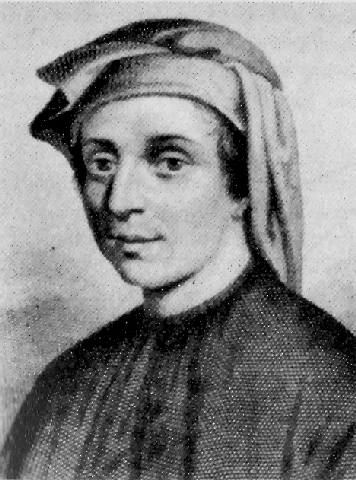
\includegraphics[scale=1]{figuren/rijen/Fibonacci.jpg} 
\caption{Leonardo van Pisa a.k.a Fibonacci ca. 1170--ca. 1250}
\end{figure}
Leonardo Fibonacci was een wiskundige die rond 1200 leefde. Hij stelde volgend probleem:
\begin{quote}
Een konijnenpaar begint zich twee maanden na de geboorte voort te planten en werpt van dan af maandelijks een nieuw konijnenpaar. De nakomelingen planten zich op dezelfde manier voort. Hoeveel konijnenparen zijn er na $n$ maanden?
\end{quote}

Fibonacci rekende uit dat het aantal aanwezige konijnenparen in een maand gelijk is aan 1, 1, 2, 3, 5, 8, 13, 21, 34, 55, \dots  \ We noemen deze rij de `rij van Fibonacci' ofwel de `Konijnenrij'.


\subsubsection*{Enkelvoudige intrest}
\begin{quote}
    We zetten een kapitaal van \euros{10\,000} op een spaarboekje met
    jaarlijkse intrest van \SI{6}{\percent}. Wat zijn de kapitalen jaar
    na jaar  tegen enkelvoudige intrest, d.w.z.\ de intrest
    wordt steeds berekend op het beginkapitaal?
\end{quote}
\label{page:intrest}
De groei van het gespaarde kapitaal (kapitaal plus intrest) jaar na jaar vind je in tabel~\ref{tbl:enkelv_intrest}. `Enkelvoudig intrest' kan je je als volgt voorstellen: je laat het beginbedrag op de rekening staan, maar de intrest neem je elk jaar mee naar huis.

\begin{table}[htb]
    \centering
    \caption{Gespaarde kapitaal bij enkelvoudige intrest per jaar}
    \begin{tabular}{cccc}
    \toprule
    jaar & & gespaarde kapitaal & \\
    \midrule
    0  	& $k_0$		&	\num{10000}	&	\\
    1	&	$k_1$	&	\num{10600}	&	$+600$\\
    2	&	$k_2$	&	\num{11200}	&	$+600$\\
    3	&	$k_3$	&	\num{11800}	&	$+600$\\
    \bottomrule
     \end{tabular}
    \label{tbl:enkelv_intrest}
\end{table}

De getallen in de derde kolom vormen een opsomming van  getallen die in een bepaalde volgorde voorkomen. Het is een \emph{rij}. Het gespaarde kapitaal bij enkelvoudige intrest per jaar is dus een rij $k_i$ waarbij $i$ aangeeft welk jaar het betreft. Met het eerste element $k_0$ doelen we op het beginkapitaal. Ieder element kan berekend worden uit het voorgaande element door er 600 bij op te tellen (figuur~\ref{fig:enkelvintrest1}).
\begin{figure}[htbp]
    \centering
\begin{tikzpicture}[x=2.5cm]
\draw[->] (-0.2,0) -- (3.5,0) node [at end, above] {$t$};
\foreach \x/\y in {0/\num{10000},1/\num{10600},2/\num{11200},3/\num{11800}}{
	\draw[shift={(\x,0.0)}] (0pt,2pt) -- (0pt,-2pt) node[above=4pt] {\small $\x$};
	\node (\x) [below=4pt] at (\x,0) {\y};
}
\foreach \x/\y in {0/1,1/2,2/3}
	\draw[-latex,red] (\x) to [bend right]  node [below] {$+600$} (\y);
\end{tikzpicture}
    \caption{Groei van kapitaal van \euros{10\,000}, \emph{enkelvoudige} intrest van \SI{6}{\percent}}
    \label{fig:enkelvintrest1} 
\end{figure}

\subsubsection*{Samengestelde intrest}
\begin{quote}
   We zetten opnieuw een kapitaal van \euros{10\,000} op een spaarboekje met
    jaarlijkse intrest van \SI{6}{\percent}. Wat zijn de kapitalen jaar
    na jaar tegen samengestelde intrest, waarbij de intrest telkens bij het vorige
    kapitaal opgeteld wordt zodat die mee intrest kan opbrengen?
\end{quote}

We stellen opnieuw een tabel op (tabel~\ref{tbl:samengest_intrest}). De getallen in de derde kolom zijn weer een rij. Het gespaarde kapitaal bij samengestelde intrest per jaar is een rij $m_i$. Het getal $m_0$ is het beginkapitaal. Ieder element kan berekend worden uit het voorgaande element door het te vermenigvuldigen met \num{1.06}.

\begin{table}[htb]
    \centering
    \caption{Gespaarde kapitaal bij samengestelde intrest per jaar}
    \begin{tabular}{cccc}
    \toprule
    jaar & & gespaarde kapitaal & \\
    \midrule
    0  	& 	$m_0$		&	$10\,000$	&	\\
    1	&	$m_1$	&	$\num{10000}+\num{0,06}\cdot\num{10000}=\num{10600}$	&	$\cdot \num{1.06}$\\
    2	&	$m_2$	&	$\num{10600}+\num{0,06}\cdot\num{10600}=\num{11236}$	&	$\cdot \num{1.06}$\\
    3	&	$m_3$	&	$\num{11236}+\num{0,06}\cdot\num{11236}=\num{11910.16}$	&	$\cdot \num{1.06}$\\
    \bottomrule
     \end{tabular}
    \label{tbl:samengest_intrest}
\end{table}


\begin{figure}[htbp]
    \centering
\begin{tikzpicture}[x=2.5cm]
\draw[->] (-0.2,0) -- (3.5,0) node [at end, above] {$t$};
\foreach \x/\y in {0/\num{10000},1/\num{10600},2/\num{11236},3/\num{11910,16}}{
	\draw[shift={(\x,0.0)}] (0pt,1pt) -- (0pt,-2pt) node[above=4pt] {\small $\x$};
	\node (\x) [below=4pt] at (\x,0) {\y};
}
\foreach \x/\y in {0/1,1/2,2/3}
	\draw[-latex,red] (\x) to [bend right]  node [below] {$\cdot \num{1,06}$} (\y);
\end{tikzpicture}
    \caption{Groei van kapitaal van \euros{10\,000}, \emph{samengestelde} intrest van \SI{6}{\percent}}
    \label{fig:enkelvintrest} 
\end{figure}

\section{Rekenkundige rij}
\label{sec:RR}
In het tweede voorbeeld van sectie~\ref{subsec:voorbeelden_rijen} (enkelvoudige intrest) hebben we gezien dat 
het gespaarde kapitaal bij enkelvoudige intrest per jaar een rij $k_i$ is met een specifiek patroon:  ieder element kan berekend worden uit het voorgaande element door er 600 bij op te tellen.

Dit patroon komt vaak voor bij rijen en
krijgt daarom de speciale naam \textit{rekenkundige rij}. De definitie
van rekenkundige rij is de volgende:


\subsection{Definitie}
\begin{quote}
Een rekenkundige rij is \emph{een rij waarbij elke term de som is van de vorige term en een constant getal $v$ (het verschil van de rij).}
\end{quote}
\begin{displaymath}
   t_1, t_2, t_3, \dots  \mbox{ is een \emph{rekenkundige
    rij}}
\end{displaymath}
\begin{displaymath}
    \Updownarrow
\end{displaymath}
\begin{displaymath}
    t_{2}-t_{1}=t_{3}-t_{2}=\dots=t_{n}-t_{n-1} =v
\end{displaymath}

Uit deze definitie leiden we af dat een rekenkundige rij volledig bepaald is door het verschil $v$ en het eerste element van de rij. Omdat $t_n=t_{n-1}+v$, is het $n$-de element van de rij gegeven door 
    \begin{equation}
        t_{n}=t_{1}+(n-1)\cdot v
        \label{eq:algelementrr}
    \end{equation}
Het verschil $v$ kunnen we berekenen als we twee willekeurige elementen van de rij kennen met hun rangnummer:
\[
  t_{n}=t_{u}+(n-u)\cdot v
\]

\subsection{Som van elementen van een een rekenkundige rij}
In heel wat toepassingen komt de \emph{som
van opeenvolgende elementen van een rekenkundige rij} voor.  Een dergelijke som
noemen we \emph{par\-tieel\-som} en noteren we door $S_{n}$,
waarbij $n$ duidt op het \emph{aantal} termen in de som. Omwille van het specifieke verband tussen de termen van de som, kunnen we een formule zoeken voor $S_{n}$.

We schrijven de som van die $n$ termen op 2 manieren op: van links naar
rechts en omgekeerd. We tellen lid aan lid op.
\begin{displaymath}
    \begin{array}{ccccccccccc}
    S_{n} & = & t_{1} & + & t_{2} & + & t_{3} & + &
    \ldots & + & t_{n}  \\
    S_{n} & = & t_{n} & + & t_{n-1} & + & t_{n-2} & + &
    \ldots & + & t_{1}  \\
    \hline
    2\cdot S_{n} & = & (t_{1}+t_{n}) & + & (t_{2}+t_{n-1}) & + &
    (t_{3}+t_{n-2}) & + & \ldots & + & (t_{n}+t_{1})
\end{array}
\end{displaymath}
In deze laatste regel zijn alle uitdrukkingen tussen de haakjes aan
elkaar gelijk.
Immers:
\begin{align*}
    t_{2}+t_{n-1} &=  (t_{1}+ v)+(t_{n}-v)=t_{1}+t_{n} \\
    t_{3}+t_{n-2} &=  (t_{1}+2\cdot v)+(t_{n}-2\cdot v)= t_{1}+t_{n} \\
     \vdots & 
\end{align*}
Bovendien zijn er juist $n$ termen met haakjes.
Vullen we deze gegevens in in de laatste uitdrukking $2\cdot S_{n}$
dan vinden we
\begin{align*}
    2\cdot S_{n} &=  n\cdot (t_{1}+t_{n})  \\
    S_{n} &= \frac{n}{2}\cdot (t_{1}+t_{n})=n \cdot \frac{t_{1}+t_{n}}{2}
  \end{align*}

\section{Meetkundige rij}
\label{sec:MR}
In het derde voorbeeld van sectie \ref{subsec:voorbeelden_rijen} (samengestelde intrest) hebben we gezien dat het gespaarde kapitaal bij samengestelde  intrest per jaar een rij $m_i$ is waarbij de elementen volgend patroon vertonen:  ieder element kan berekend worden uit het voorgaande element door het te vermenigvuldigen met \num{1.06}.

Dit patroon van vermenigvuldigen komt vaak voor bij rijen en krijgt daarom de speciale naam \emph{meetkundige  rij}. De definitie van meetkundige rij is de volgende:
\subsection{Definitie}
\begin{quote}
Een meetkundige rij is \emph{een rij waarbij elke term het product is van de vorige term en een constant getal $r$ (de \emph{reden}, ook wel het \emph{quotiënt} genoemd).}
\end{quote}
    \begin{displaymath}
             t_1, t_2, t_3, \dots 
        \mbox{ is een meetkundige rij}
    \end{displaymath}
    \begin{displaymath}
         \Updownarrow
    \end{displaymath}
    \begin{displaymath}
         \frac{t_{2}}{t_{1}}=\frac{t_{3}}{t_{2}}=\dots =\frac{t_{n}}{t_{n-1}}=r
    \end{displaymath}

Een meetkundige rij is volledig bepaald door zijn eerste element en de reden~$r$. Omdat $t_n=t_{n-1}\cdot r$, is het $n$-de element van de rij gegeven door
\begin{equation}
\label{eq:rec_mr}
t_n=t_1\cdot r^{n-1}.
\end{equation}
De reden $r$ kunnen we berekenen als we twee willekeurige elementen van de rij kennen met hun rangnummer:
\[
t_n=t_u\cdot r^{n-u}
\]

\subsection{Som van elementen van een meetkundige rij}\label{subsec.Tn}
In heel wat problemen uit de financi\"{e}le algebra komt de som van
opeenvolgende elementen van een meetkundige rij voor. Dergelijke som noemen we
opnieuw een partieelsom van de rij en noteren we door $T_{n}$,
waarbij $n$ duidt op het aantal termen in de som. In wat volgt zoeken we een formule voor $T_{n}$.


Het vertrekpunt is de som van de $n$ opeenvolgende termen van de meetkundige rij. We
vermenigvuldigen beide leden van die uitdrukking met $r$. Daarna
trekken we lid aan lid af.
\begin{align*}
    T_{n} &=  t_{1}+t_{2}+t_{3}+\dots +t_{n-1}+t_{n}  \\
    r\cdot T_{n} &= r\cdot t_{1}+r\cdot t_{2}+r\cdot t_{3}+\dots +r\cdot
    t_{n-1}+r\cdot t_{n}  \\ \hline \\
    T_{n}-r\cdot T_{n} &= t_{1}+(t_{2}-r\cdot t_{1})+ (t_{3}-r\cdot
    t_{2})+ \dots +(t_{n}-r\cdot t_{n-1})-r\cdot t_{n}
\end{align*}

Ui vergelijking (\ref{eq:rec_mr}) volgt dat alle termen tussen haakjes gelijk zijn aan 0. Na vereenvoudiging vinden we uit de
laatste vergelijking een formule voor $T_{n}$.
\begin{align*}
    T_{n}-r\cdot T_{n} &= t_{1}-r\cdot t_{n}  \\
    (1-r)\cdot T_{n} &=  t_{1}-r\cdot t_{n} \\
    T_{n} &= \frac{t_{1}-r\cdot t_{n}}{1-r}  \\
    T_{n} &= \frac{t_{1}-r\cdot r^{n-1} \cdot t_{1}}{1-r}\\
    T_{n} &= \frac{t_{1}\cdot (1-r^{n})}{1-r}=\frac{t_{1}\cdot
    (r^{n}-1)}{r-1}
\end{align*}


De reden $r$ moet vanzelfsprekend voldoen aan $r\neq 1$. Het geval $r=1$ is namelijk een weinig interessante rij
want alle elementen zijn dan aan elkaar gelijk. 


\section{Rijen en financi\"{e}le algebra}
In deze paragraaf gaan we dieper in op toepassingen van rijen in de
financi\"{e}le algebra. In alle voorbeelden draait het om \textit{samengestelde intrest}.
\begin{figure}[h]
\begin{center}
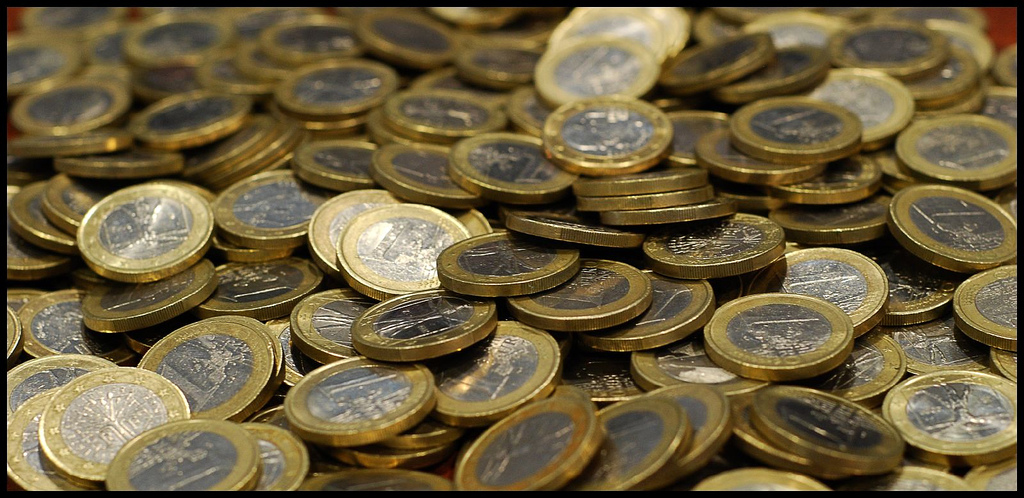
\includegraphics[trim=0.2cm 1.5cm 0.2cm 1.5cm,clip,width=\textwidth]{figuren/rijen/geldstukken.jpg}
\end{center}
\end{figure}



\subsection{Gespaarde kapitaal is een meetkundige rij}
In sectie~\ref{sec:MR}  merkten we op dat het gespaarde kapitaal bij samengestelde intrest per jaar een meetkundige rij is. Bij het derde voorbeeld van sectie~\ref{subsec:voorbeelden_rijen} (op pagina~\pageref{subsec:voorbeelden_rijen}) gaat het om  een meetkundige rij $m_i$ met reden $r=\num{1.06}$ en eerste element $m_0=\num{10000}$. Uit vergelijking~(\ref{eq:rec_mr}) volgt dat een algemeen element $m_j$ dat het gespaarde kapitaal in jaar $j$ weergeeft gelijk is aan 
\begin{equation}
m_j=m_0\cdot r^j=m_0\cdot\num{1.06}^j.
\label{eq:samengest_intrest}
\end{equation}  
We kunnen vergelijking~(\ref{eq:samengest_intrest}) gebruiken om snel te berekenen hoe groot het kapitaal is na bijvoorbeeld 13 jaar:
\[
m_{13}=\num{10000}\cdot\num{1.06}^{13}=\num{21329,28}
\]
We herinneren je even aan vergelijking~(\ref{eq:si}):
\begin{equation}
     K(t)=K(0)\cdot g^{t}=1000\cdot \num{1.07}^{t}
    \label{eq:si2}
\end{equation}
Merk op dat deze vergelijking sterk gelijkt op vergelijking~(\ref{eq:samengest_intrest}). Het belangrijkste verschil bestaat erin dat de index $j$ in vergelijking~(\ref{eq:samengest_intrest}) een geheel getal is, terwijl dat niet zo is in vergelijking~(\ref{eq:si2}). Hieruit besluiten we dat een meetkundige rij met reden $r$ het discrete geval is van een exponentieel groeiproces met groeifactor $r$. 

Wanneer het financi\"ele algebra betreft, maken we geen strikt onderscheid tussen de vergelijking van een meetkundige rij en die van een exponentieel groeiproces. Zo zullen we vergelijking~(\ref{eq:samengest_intrest}) ook gebruiken om te berekenen hoe groot het kapitaal is na bijvoorbeeld anderhalf jaar ($\num{10000}\cdot \num{1.06}^{\num{1.5}}$) of 5 jaar geleden ($\num{10000}\cdot \num{1.06}^{-5}$). 

Voor een exponentieel groeiproces bepaalden we het verband tussen procentuele toename en groeifactor in vergelijking~\eqref{eq:groeifactor_procent}. Op gelijkaardige manier vind je dat de reden van de meetkundige rij bepaald door het gespaarde kapitaal met intrest $i$ gelijk is aan $r=1+i$. 

\subsection{Belangrijke principes uit de financi\"{e}le
algebra}\label{sec.principes}
We brengen enkele belangrijke principes onder de aandacht:
\begin{itemize}
       \item Zichtrekeningen brengen \textit{elke dag} intrest. Als je je spaargeld bijvoorbeeld op 1 februari naar de bank brengt en het terug afhaalt op 21 februari, krijg je voor die 20 dagen ($=20/365$ste van een jaar) intrest.
    \item Kapitaal dat uitstaat tegen samengestelde intrest
      \emph{vermeerdert} in waarde als we verder gaan in de tijd.
       \item Bedragen kan je alleen met elkaar \emph{vergelijken (of optellen)}
       als je ze
       verrekent naar \emph{eenzelfde} tijdstip.
   \end{itemize}

\subsection{Voorbeeld: Samengestelde intrest}
\begin{quote}
Je zet op 1 januari 2012 een bedrag $K$ op een spaarrekening met jaarlijkse intrest \SI{3}{\percent}. Hoe groot moet $K$ zijn opdat er na 3 jaar \euros{100} op de spaarrekening zal staan?
\end{quote}
\subsubsection{Voorbeeld 1: Eerste manier}
\begin{figure}[htbp]
    \centering
\begin{tikzpicture}[x=2.5cm]
\draw[->] (-0.2,0) -- (3.5,0) node [at end, above] {$t$};
\foreach \x/\y in {2012/$K$?,2013/$\cdots$ ,2014/$\cdots$ ,2015/\num{100}}{
	\draw[shift={(\x-2012,0.0)}] (0pt,1pt) -- (0pt,-2pt) node[above=4pt] {\small $\x$};
	\node (\x) [below=4pt] at (\x-2012,0) {\y};
}
\foreach \x/\y in {0/1,1/2,2/3}
	\draw[-latex,red] (\x) to [bend right]  node [below] {$\cdot \num{1,03}$} (\y);
\end{tikzpicture}
    \caption{Welk kapitaal is na drie jaar aangegroeid tot \euros{100} tegen een WR van \SI{3}{\percent}?}
    \label{fig:oef1verdertellen} 
\end{figure}
We stellen de gegevens en het gevraagde voor in figuur~\ref{fig:oef1verdertellen}.

Het gespaarde kapitaal jaar na jaar vormt een meetkundige rij  met volgende kenmerken:
\begin{itemize}
\item begintijdstip 1 januari 2012
\item eerste element $m_0=K$
\item periode 1 jaar
\item reden $r=1+\dfrac{3}{100}=\num{1.03}$
\end{itemize}
zodat het gespaarde kapitaal na $j$ jaar gelijk is aan 
\begin{equation}
m_j=K\cdot \num{1.03}^j.
\label{eq:sam_intrest_vb1}
\end{equation}

Uit het gegeven blijkt dat $m_3=100$. We vullen dit in vergelijking~(\ref{eq:sam_intrest_vb1}) in:
\begin{align*}
100&=K\cdot \num{1.03}^3\\
&\Updownarrow\\
K&=\dfrac{100}{\num{1.03}^3}=\num{96,80}
\end{align*}
Omdat kapitaal dat uitstaat tegen een samengestelde intrest altijd vermeerdert, moet $K$ kleiner zijn dan 100, wat we inderdaad bekomen.

\subsubsection{Voorbeeld 1: Tweede manier}
\label{vb1:2demanier}
Je kan  het vorige voorbeeld ook oplossen door terug te gaan in de tijd. Je neemt dan als begintijdstip van de rij 1 januari 2015. 
\begin{figure}[htbp]
    \centering
\begin{tikzpicture}[x=2.5cm]
\draw[->] (-0.2,0) -- (3.5,0) node [at end, above] {$t$};
\foreach \x/\y in {2012/$K$?,2013/$\cdots$ ,2014/$\cdots$ ,2015/\num{100}}{
	\draw[shift={(\x-2012,0.0)}] (0pt,1pt) -- (0pt,-2pt) node[above=4pt] {\small $\x$};
	\node (\x) [below=4pt] at (\x-2012,0) {\y};
}
\foreach \x/\y in {3/2,2/1,1/0}
	\draw[-latex,red] (\x) to [bend left]  node [below] {$: \num{1,03}$} (\y);
\end{tikzpicture}
    \caption{Welk kapitaal is na drie jaar aangegroeid tot \euros{100} tegen een WR van \SI{3}{\percent}?}
    \label{fig:oef1terugtellen} 
\end{figure}
De rij heeft dan volgende kenmerken:
\begin{itemize}
\item begintijdstip 1 januari 2015
\item eerste element $n_0=100$
\item periode 1 jaar
\item reden $r=1+\dfrac{3}{100}=\num{1.03}$
\end{itemize}
zodat het gespaarde kapitaal na $i$ jaar (sinds 1 januari 2015) gelijk is aan 
\begin{equation}
n_i=100\cdot \num{1.03}^i
\end{equation}
Om het kapitaal op 1 januari 2012 te kennen, moeten we $n_{-3}$ berekenen, dat gelijk is aan 
\[
K=100\cdot \num{1.03}^{-3}=\frac{100}{\num{1.03}^{3}}=\num{96,80}.
\]


\subsubsection{Voorbeeld 2}
\begin{quote}
Op spaarrekening A (jaarlijkse rente \SI{3}{\percent}) stort je op 1 januari 2010 \euros{100}. Op spaarrekening B (jaarlijkse rente \SI{2,5}{\percent}) stort je op 10 januari 2012 \euros{110}. Wanneer is het bedrag op beide spaarrekeningen gelijk?
\end{quote}
\noindent
Voor beide rekeningen vormt het gespaarde kapitaal een meetkundige rij:
\begin{multicols}{2}
\begin{itemize}
\item begintijdstip 1 januari 2010
\item eerste element $a_0=100$
\item periode 1 jaar
\item reden $r=1+\dfrac{3}{100}=\num{1.03}$
\end{itemize}
zodat het gespaarde kapitaal na $j$ jaar gelijk is aan 
\begin{equation}
a_j=100\cdot \num{1.03}^j
\label{eq:sam_intrest_vb2a}
\end{equation}
met $j$ het aantal jaar sinds 1/1/10.
\begin{itemize}
\item begintijdstip 1 januari 2012
\item eerste element $b_0=110$
\item reden $r=1+\dfrac{\num{2.5}}{100}=\num{1.025}$
\end{itemize}
zodat het gespaarde kapitaal na $k$ jaar gelijk is aan 
\begin{equation}
b_k=110\cdot \num{1.025}^k
\label{eq:sam_intrest_vb2b}
\end{equation}
met $k$ het aantal jaar sinds 1/1/12

\end{multicols}
\begin{figure}[htpb]
\centering
\begin{tikzpicture}[x=1.6cm]
%\draw[dashed] (6,-1) -- (6,3);
%% onderste tijdsas
\draw[->] (-0.2,0) -- (6.5,0) node [at end, above] {$t$};
\foreach \x in {2010,...,2014}{
	\draw[shift={(\x-2010,0.0)}] (0pt,1pt) -- (0pt,-2pt) node[above=4pt] {\small $\x$};
	}
	\draw (6,1pt) -- (6, -2pt) node[above=4pt] {?};
	\node (t12) [below=4pt,blue] at (2,0) {110};
\node (t13)  at (3,-0.4) {};	
\node (t14)  at (4,-0.4) {};
\node (t15)  at (5,-0.4) {};
\node (t16)[below=4pt,blue]  at (6,0) {$K$};
	\draw[-latex,red] (t12) to [bend right]  node [below] {$\cdot \num{1,025}$} (t13);
		\draw[-latex,red] (t13) to [bend right]  node [below] {$\cdot \num{1,025}$} (t14);
			\draw[-latex,red] (t15) to [bend right]  node [below] {$\cdot \num{1,025}$} (t16);
			
%% Deel 2 (bovenste) van de figuur			
\draw[->] (-0.2,2) -- (6.5,2) node [at end, above] {$t$};
\foreach \x in {2010,...,2014}{
	\draw[shift={(\x-2010,2.0)}] (0pt,1pt) -- (0pt,-2pt) node[above=4pt] {\small $\x$};
	}
\draw[shift={(0,2)}] (6,1pt) -- (6, -2pt) node[above=4pt] {?};
\node (tt10) [below=4pt,blue] at (0,2) {100};
\node (tt11)  at (1,1.6) {};	
\node (tt12)  at (2,1.6) {};
\node (tt13)  at (3,1.6) {};
\node (tt14)  at (4,1.6) {};
\node (tt15)  at (5,1.6) {};
\node (tt16)[below=4pt,blue]  at (6,2) {$K$};
\draw[-latex,red] (tt10) to [bend right]  node [below] {$\cdot \num{1,03}$} (tt11);
\draw[-latex,red] (tt11) to [bend right]  node [below] {$\cdot \num{1,03}$} (tt12);
\draw[-latex,red] (tt12) to [bend right]  node [below] {$\cdot \num{1,03}$} (tt13);
\draw[-latex,red] (tt13) to [bend right]  node [below] {$\cdot \num{1,03}$} (tt14);
\draw[-latex,red] (tt15) to [bend right]  node [below] {$\cdot \num{1,03}$} (tt16);
\end{tikzpicture}
\caption{Voorbeeld 2: wanneer zelfde eindbedrag?}
\end{figure}
Bij het oplossen van het vraagstuk moeten we rekening houden met het verschil in begintijdstip. Spaarrekening B heeft altijd 2 jaar minder intrest opgebracht dan rekening A. We moeten dus volgende vergelijking oplossen: Zoek $t$ zodat 
\begin{align*}
a_t&=b_{t-2}\\
&\Updownarrow \\
100\cdot \num{1.03}^t&=110\cdot \num{1.025}^{t-2}\\
&=110\cdot \num{1.025}^{-2}\cdot \num{1.025}^t\\
&\Updownarrow \\
\left(\frac{\num{1.03}}{\num{1.025}}\right)^t&=\frac{110\cdot \num{1.025}^{-2}}{100} \\
&\Updownarrow \\
t&=\frac{\log\left(\dfrac{110\cdot \num{1.025}^{-2}}{100}\right)}{\log\left(\dfrac{\num{1.03}}{\num{1.025}}\right)}
\end{align*}


\subsection{Rente en periode}
Geld wordt niet altijd per jaar belegd. Stel dat je bank je laat kiezen uit twee zichtrekeningen:
\begin{enumerate}
\item Bij zichtrekening A krijg je maandelijks \SI{0,5}{\percent} intrest
\item Bij zichtrekening B krijg je jaarlijks \SI{6}{\percent} intrest
\end{enumerate}
Je hebt \euros{100}. Welk van beide zichtrekeningen is de meest interessante?


We bepalen de meetkundige rijen die horen bij beide zichtrekeningen en het  bedrag dat op de rekening staat na 1 jaar.

\subsubsection{Zichtrekening A}
\begin{itemize}
\item periode: 1 maand
\item reden: $1+\num{0.5}/100=\num{1.005}$
\item beginwaarde $a_0=100$
\end{itemize}
Bijhorende meetkundige rij:
\begin{equation}
a_i=100\cdot \num{1.005}^i \quad \text{met~}i\text{~uitgedrukt~in~maanden.}
\end{equation}
E\'en jaar duurt 12 maanden, dus na 1 jaar staat volgend bedrag op de rekening:
\[
a_{12}=100\cdot \num{1.005}^{12}=106,168
\]


\subsubsection{Zichtrekening B}
\begin{itemize}
\item periode: 1 jaar
\item reden: $1+\frac{6}{100}=1.06$
\item beginwaarde $a_0=100$
\end{itemize}
Bijhorende meetkundige rij:
\begin{equation}
b_j=100\cdot \num{1.06}^j \quad \text{met~}j\text{~uitgedrukt~in~jaren}
\end{equation}
Na 1 jaar staat volgend bedrag op de rekening:
\[
b_1=100\cdot \num{1.06}^1=106
\]

Het bedrag op zichtrekening A is (een beetje) groter, dus zichtrekening A is de meest interessante belegging. Nochtans is de jaarlijkse intrest op zichtrekening B juist 12 keer groter dan de maandelijkse intrest op zichtrekening A. Als de periode verandert met een bepaalde factor, mag je de rente dus \textit{niet} met diezelfde factor vermenigvuldigen. Je moet \emph{eerst} de reden van bijhorende meetkundige rij (met de nieuwe periode) bepalen en van daaruit de rente berekenen. Maak daarbij gebruik van figuur~\ref{fig:periode_factor}.



\subsection{Voorbeeld: Periodiek sparen} 
\label{vb:persparen}

In paragraaf \ref{subsec.Tn} werd volgende formule afgeleid:
\begin{equation}
    T_{n}=t_{0}\cdot \frac{r^{n}-1}{r-1}=t_{0}\cdot \frac{1-r^{n}}{1-r}
    \label{eq:sommr}
\end{equation}
$T(n)$ is de som van $n$ termen van een meetkundige rij met reden
$r$ en eerste term $t_{0}$. In deze paragraaf laten we zien hoe
deze formule gebruikt wordt in financi\"ele algebra. 

\begin{quote}
    Jan wil over 5 jaar een brommer kopen. Daarvoor moet hij over 5
    jaar beschikken over een bedrag van \euros{1750}. Hij begint nu te
    sparen en zet elk \emph{semester} \euros{125} op een rekening met
    samengestelde intrest. De semestri\"{e}le intrest is \SI{5}{\percent}.
    Zal Jan over 5 jaar over voldoende kapitaal beschikken om
    die brommer te kopen?
\end{quote}

\subsubsection{Stap 1: Tijdsas}
We beginnen met de situatie te visualiseren. Daartoe tekenen we een tijdsas waarop we alle gebeurtenissen aanduiden: tijdstippen waarop iets gebeurt, wat er gebeurt (storting), tijdstip waarnaar gerekend moet worden. Dit wordt getoond in figuur~\ref{fig:t1}. 

    \begin{figure}[htb]
            \centering

\begin{tikzpicture}[x=1cm]
\draw[->] (-0.2,0) -- (10.5,0) node [at end, above] {$t$};
\foreach \x in {0,...,10}{
	\draw[shift={(\x,0.0)}] (0pt,1pt) -- (0pt,-2pt);
	\draw[shift={(\x,0.0)},-latex] (0,-0.7) -- (0,-0.2);
	}
\foreach \x in {0,...,5}{
	\node at ({\x*2},0.3) {\x};
}
\node[red] at (0,-1) {125};
\node[orange] at (1,-1) {125};
\node[green] at (2,-1) {125};
\foreach \x in {3,...,9}{
	\node at (\x,-1) {125};
}
\node[blue] at (10,-1) {125};
\end{tikzpicture}

        \caption{Semestri\"{e}le stortingen van \euros{125}}
        \label{fig:t1}
    \end{figure}
    \setcounter{tijd}{0}

\subsubsection{Stap 2: Periode en groeifactor bepalen}
In het vraagstuk werken we met samengestelde intrest. Het gespaarde kapitaal neemt elke periode toe met een zelfde groeifactor. Deze factor hangt af van de periode. We moeten beide dus bepalen:
\begin{itemize}
\item de periode is 1 semester
\item de factor is  $r=\num{1.05}$ ($=1+\frac{5}{100}$).
\end{itemize}


\subsubsection{Stap 3: Gespaarde bedragen berekenen}
 Elk semester neemt het gespaarde kapitaal toe met factor $\num{1.05}$. Bovendien stort Jan elke semester \euros{125}. De semestri\"ele rekeninguittreksels van de spaarrekening van Jan zouden er dus kunnen uitzien als in tabel~\ref{tab:persparen}.
\begin{table}[htbp]
\centering
\caption{Gespaarde kapitaal per semester}
\begin{tabular}{cl}
\toprule
semester  & gespaarde kapitaal\\
\midrule
0 & $\textcolor{red}{125}$ \\
1 & $\textcolor{red}{125}\cdot \num{1.05}+\textcolor{orange}{125}$\\
2 & $(\textcolor{red}{125}\cdot \num{1.05}+\textcolor{orange}{125})\cdot \num{1.05}+\textcolor{green}{125}$\\ &$\qquad=\textcolor{red}{125}\cdot \num{1.05}^2+\textcolor{orange}{125}\cdot \num{1.05}+\textcolor{green}{125}$\\
3 & $(\textcolor{red}{125}\cdot \num{1.05}^2+\textcolor{orange}{125}\cdot \num{1.05}+\textcolor{green}{125})\cdot \num{1.05}+125$\\&$\qquad=\textcolor{red}{125}\cdot \num{1.05}^3+\textcolor{orange}{125}\cdot \num{1.05}^2+\textcolor{green}{125}\cdot \num{1.05}+125$\\
\dots & \dots \\
10 & $\textcolor{red}{125}\cdot \num{1.05}^{10}+\textcolor{orange}{125}\cdot \num{1.05}^9+\dots+125\cdot \num{1.05}+\textcolor{blue}{125}$\\
\bottomrule
\end{tabular}
\label{tab:persparen}
\end{table}

De som na 10 semesters kan je ook als volgt bekijken: 
\begin{itemize}
\item de \euros{\textcolor{red}{125}} die gestort worden op semester 0 staan 10 semesters op de rekening. Hun aandeel in het gespaarde kapitaal is gelijk aan $125\cdot \num{1.05}^{10}$
\item de \euros{\textcolor{orange}{125}} die gestort worden op semester 1 staan 9 semesters op de rekening. Hun aandeel in het gespaarde kapitaal is gelijk aan $125\cdot \num{1.05}^{9}$
\item \dots
\item de laatste \euros{\textcolor{blue}{125}} staan nog maar net op de rekening en hebben nog geen intrest opgebracht. Hun aandeel is gelijk aan 125.
\end{itemize}
In wat volgt zullen we het gespaarde bedrag steeds op deze manier berekenen. We gebruiken de figuur daartoe als hulpmiddel. Bij elk bedrag tekenen we een pijl die aangeeft met welke factor het bedrag vermenigvuldigd moet worden. 


    \begin{figure}[htb]
            \centering
\begin{tikzpicture}[x=1cm]
\draw[->] (-0.2,0) -- (10.5,0) node [at end, above] {$t$};
\foreach \x in {0,...,10}{
	\draw[shift={(\x,0.0)}] (0pt,1pt) -- (0pt,-2pt);
	\draw[shift={(\x,0.0)},-latex] (0,-0.7) -- (0,-0.2);
	}
\foreach \x in {0,...,5}{
	\node at ({\x*2},0.3) {\x};
}
\node[red] at (0,-1) {125};
\node[orange] at (1,-1) {125};
\node[green] at (2,-1) {125};
\foreach \x in {3,...,9}{
	\node at (\x,-1) {125};
}
\node[blue] at (10,-1) {125};
\draw[-latex,red] (0,0) to  [out=50,in=130]  node [above] {$\cdot \num{1,05}^{10}$} (10,0);
\draw[-latex,orange] (1,0) to  [out=40,in=140]  node [above] {$\cdot \num{1,05}^{9}$} (10,0);
\draw[-latex,green] (2,0) to  [bend left]  node [below] {$\cdot \num{1,05}^{8}$} (10,0);
\end{tikzpicture}
        \caption{Semestri\"{e}le stortingen van \euros{125}}
        \label{fig:tt1}
    \end{figure}
    \setcounter{tijd}{0}


\subsubsection{Stap 4: Som van elementen van een meetkundige rij}
In de vorige stap berekenden we dat Jan volgend bedrag gespaard zal hebben:
\begin{equation}
K= 125\cdot \num{1.05}^{10}+125\cdot \num{1.05}^9+\dots+125\cdot \num{1.05}+125
\label{eq:som_vb2}
\end{equation}
Wanneer we de termen van de som bekijken, merken we op dat het elementen zijn van een meetkundige rij met volgende kenmerken:
\begin{itemize}
\item eerste term $t_0=125\cdot \num{1.05}^{10}$
\item reden $r=\dfrac{t_1}{t_0}=1/\num{1.05}$
\item aantal\footnote{Opgepast: dit is een bron van
    fouten. Tussen 0 en 10 liggen 10 stappen, maar het zijn in totaal 11
    getallen. Kijk dus in oefeningen altijd goed na of je je niet 1
    eenheid vergist!} elementen: 11
\end{itemize}
Als we gebruik maken van vergelijking~\eqref{eq:sommr} vinden we eenvoudig
\begin{equation}
K=125\cdot\num{1.05}^{10}\cdot \dfrac{1-\left(\frac{1}{\num{1.05}}\right)^{11}}    {1-\frac{1}{\num{1.05}} }
\end{equation}

Het staat je vrij om de termen van som~(\ref{eq:som_vb2}) te herschikken, bijvoorbeeld
\begin{equation}
K=125 +125\cdot \num{1.05}+\dots+125\cdot \num{1.05}^9+125\cdot \num{1.05}^{10}
\label{eq:som_vb2_anders}
\end{equation}
De reden is dan geen breukgetal meer:
\begin{itemize}
\item eerste term $s_0=125$
\item reden $r=\dfrac{s_1}{s_0}=\num{1.05}$
\item aantal termen: 11
\end{itemize}
zodat de somformule een eenvoudigere uitdrukking is 
\begin{equation}
K=125\cdot \frac{1-\num{1.05}^{11}} {1-\num{1.05}}
\label{eq:som_vb2bis}
\end{equation}
Reken zelf uit dat vergelijking~(\ref{eq:som_vb2}) en (\ref{eq:som_vb2bis}) aan mekaar gelijk zijn. 

\subsubsection{Stap 5: Antwoord formuleren}
Als je vergelijking~(\ref{eq:som_vb2}) berekent, vind je $K=1776$. Jan heeft  meer gespaard dan nodig en dus kan hij de brommer kopen.

\subsection{Periodiek sparen en lenen: Algemene werkwijze}

We veralgemenen de werkwijze die we in de vorige sectie uitgerold hebben. 

\subsubsection{1. Tijdsas}
Stel de gegevens schematisch voor op een tijdsas.
\begin{itemize}
\item Geef de as een richting (pijl) en noteer in welke tijdseenheid je
werkt (bijvoorbeeld jaren of maanden).
\item Je mag de as onderbreken met puntjes.
\item Duid aan wat er wanneer gebeurt: op welke tijdstippen wordt er geld
gestort/afgehaald? 	
\item Duid het tijdstip $T$ aan waarnaar je rekent.
\end{itemize}

\subsubsection{2.	Periode en reden}
Noteer de periode waarin je de berekeningen zal doen. Bereken de bijbehorende reden. Vermijd afrondingen. Werk liever met $\sqrt{\num{1.05}}$ dan met $\num{1.02469507}$.

\subsubsection{3.	Gespaarde bedragen}
Duid op de tijdsas met behulp van pijlen aan hoe de bedragen veranderen als je ze omrekent naar het tijdstip $T$.

\subsubsection{4. Som}
In de meeste opgaven moet je een som berekenen.
\begin{itemize}
\item Schrijf de som volledig uit.  Dit wil zeggen: eerste, tweede en laatste
term;
\item 	Indien je de som maakt van elementen van een meetkundige rij,
noteer dan
\begin{itemize}
\item het eerste element $t_0$; 
\item de reden $r$; 
\item het aantal elementen van de rij.
\end{itemize}
\item 	Pas de somformule toe. 	
\item Bereken de waarde van de som bijvoorbeeld met Scilab.
\end{itemize}

\subsubsection{5. Antwoord}
Formuleer het antwoord.


\subsection{Voorbeeld : Lening}
Lenen en (periodiek) sparen zijn  gelijkaardige processen: je zet op regelmatige tijdstippen geld opzij. Het belangrijke verschil is dat je bij lenen het totaalbedrag op voorhand ter beschikking hebt. Dit resulteert in een verschillende werkwijze bij oefeningen over sparen en lenen: bij sparen berekenen we de waarde van een bedrag in de toekomst; bij lenen kijken we hoeveel een bedrag een tijdje geleden waard was. 
\begin{quote}
    We lenen een bedrag van \euros{5\,000} bij de bank voor de aankoop
    van een auto. We komen overeen dat bedrag terug te betalen over
    een periode van 10 jaar, door middel van jaarlijkse \emph{constante}
    aflossingen. We nemen aan dat de jaarlijkse rente over die periode \SI{5}{\percent} is.
    De eerste afbetaling doen we \'{e}\'{e}n jaar na aankoop. Welk
    bedrag $K$ moeten we jaarlijks afbetalen?
\end{quote}
Er zijn twee verschillen met  sectie~\ref{vb:persparen}: het vraagstuk gaat over lenen \'en het eindbedrag is gekend en niet het bedrag van de jaarlijkse stortingen.

We volgen de algemene werkwijze, ervan uitgaand dat de bank
geen verlies en geen winst mag maken. Geld wordt ook niet meer in
de kous gestopt maar wordt uitgezet tegen samengestelde intrest.

\subsubsection{Stap 1: Tijdsas}
We tekenen een tijdsas, figuur~\ref{fig:t2}, waarop we de 10 jaren uitzetten.
    Onder tijdstip $t=1$ en alle volgende duiden we het bedrag $T$ aan.
    Boven tijdstip $t=0$ zetten we het ontleende bedrag $5\,000$.
    \begin{figure}[htb]
            \centering
            \begin{tikzpicture}[x=1cm]
\draw[->] (-0.2,0) -- (10.5,0) node [at end, above] {$t$};
\foreach \x in {0,...,10}{
	\draw[shift={(\x,0.0)}] (0pt,1pt) -- (0pt,-2pt);
	\node at ({\x},0.3) {\x};
	}
\foreach \x in {1,...,10}{
	\draw[shift={(\x,0.0)},-latex] (0,-0.7) -- (0,-0.2);
}
\draw[latex-] (0,-0.7) -- (0,-0.2);
\node at (0,-1) {\num{5000}};
\node[red] at (1,-1) {$T$};
\node[green] at (2,-1) {$T$};
\foreach \x in {3,...,9}{
	\node at (\x,-1) {$T$};
}
\node[blue] at (10,-1) {$T$};
\draw[-latex,red] (1,0) to  [out=150,in=30]  node [above] {$\cdot \frac{1}{ \num{1,05}}$} (0,0);
\draw[-latex,green] (2,0) to  [out=140,in=40]  node [above] {$\cdot \frac{1}{ \num{1,05}^{2}}$} (00,0);
\draw[-latex,blue] (10,0) to  [out=135,in=55]  node [below] {$\cdot \frac{1}{ \num{1,05}^{10}}=\cdot \num{1,05}^{-10}$} (0,0);
\end{tikzpicture}
        \caption{Tijdsas voor de autolening}
        \label{fig:t2}
    \end{figure}
    \setcounter{tijd}{0}

\subsubsection{Stap 2: Periode en reden}
\begin{itemize}
\item periode: 1 jaar
\item rente is \SI{5}{\percent}, dus $r=\num{1.05}$
\end{itemize}

\subsubsection{Stap 3: Gespaarde bedragen}
     Elk terugbetaald bedrag $T$ draagt bij tot het ontleende kapitaal. Omdat het ene bedrag later terugbetaald wordt dan het ander, is die bijdrage tot het kapitaal steeds verschillend. We moeten voor elke bijdrage berekenen hoeveel die waard was bij aankoop van de auto. We doen dit zoals aangegeven op blz.~\pageref{vb1:2demanier}.
     \begin{itemize}
\item het bedrag dat 1 jaar na aankoop terugbetaald werd (uitgerekend naar het referentietijdstip $t=0$): $\textcolor{red}{T\cdot \num{1.05}^{-1}}$
\item 2 jaar na aankoop: $\textcolor{green}{T\cdot \num{1.05}^{-2}}$
\item \dots
\item 10 jaar na aankoop: $\textcolor{blue}{T\cdot \num{1.05}^{-10}}$
\end{itemize}
Op de tijdsas duiden we dat aan door pijlen te trekken van de verschillende `terugbetaalmomenten' naar het begintijdstip toe. Omdat we teruggaan in de tijd, moeten we vermenigvuldigen met een \emph{negatieve} macht van de reden (of, wat op hetzelfde neerkomt, delen door de positieve macht).

\subsubsection{Stap 4: Som}
Het geleende bedrag is gelijk aan
\begin{equation}
5\,000=\textcolor{red}{T\cdot \num{1.05}^{-1}}+\textcolor{green}{T\cdot \num{1.05}^{-2}}+\dots+\textcolor{blue}{T\cdot \num{1.05}^{-10}}s
\end{equation}
Dit is een som van elementen van een meetkundige rij met volgende kenmerken:
\begin{itemize}
\item eerste term $t_0=T\cdot \num{1.05}^{-1}$
\item reden $r=\dfrac{t_1}{t_0}=\num{1.05}^{-1}$
\item aantal termen $n=10$
\end{itemize}
De som is dus gelijk aan
\begin{equation}
5\,000=T\cdot \num{1.05}^{-1}\cdot \frac{1-\left(\num{1.05}^{-1}\right)^{10}}{1-\num{1.05}^{-1}}
\end{equation}
Uit deze eerstegraadsvergelijking kunnen we $T$ oplossen:
\begin{equation}
T=\frac{5\,000}{ \num{1.05}^{-1}\cdot \dfrac{1-\left(\num{1.05}^{-1}\right)^{10}}{1-\num{1.05}^{-1}}}=\num{647.5}
\end{equation}

\subsubsection{Stap 5: Antwoord}
De lening is volledig terugbetaald
    door 10 opeenvolgende jaren \euros{\num{647.5}} te betalen aan de bank.



%\newpage 
%%%%%%%%%%%%%%%%%%%%%%%%%%%%%%%%%%%%%%%%%%%%%%%%%%%%%%%%%%%%%%%%%%%%%
% Laatste aanpassing:
% augustus 11 [Jan]: eenheden, getallen consistent gemaakt
%
%5/5/11 [Greetje]: grote kuis
%
% 9/9/02 [Jan]: inconsistentie met euro's weggewerkt.
%           
% 17/08/02 Roos
%   volgorde van de oefeningen volgens moeilijkheidsgraad of aard.
%    foute opgave "groei" verwijderd.      
%   
%   examenvragen 2002 op financi\"{e}le algebra toegevoegd.
%
% 01/09/01 door Greetje          
%%%%%%%%%%%%%%%%%%%%%%%%%%%%%%%%%


\section{Oefeningen}
\subsection{Rekenkundige en meetkundige rijen}
\begin{enumerate}
    \item  Een rekenkundige rij heeft als eerste term $4$, als tweede term $6$.
    \begin{enumerate}
        \item Bereken het verschil $v$. 
        \item Bereken de twintigste term.

        \item  Bereken de som van de eerste 40 termen.

        \item  Een som van opeenvolgende termen van die rij begint
        bij de zesde term. Hoeveel termen moet
        men optellen om als som 264 te bekomen?
    \end{enumerate}

    \item  Een rolletje toiletpapier heeft een diameter van \SI{16}{\centi\meter}. De
    diameter van het binnenste kartonnen rolletje is \SI{4}{\centi\meter}. We nemen
    aan dat het papier een dikte heeft van \SI{1}{\milli\meter}. Noem $t_{1}$ de
    lengte van de eerste winding, $t_{2}$ de lengte van de
    tweede winding enz.
    \begin{enumerate}
        \item  Hoeveel windingen bevat het rolletje
        toiletpapier?

        \item  Hoeveel meter papier is er op de rol? (omtrek
        cirkel: $2 \cdot \pi \cdot R$)
    \end{enumerate}

    \item  Gegeven de meetkundige rij $t_{n}$ met $t_{4}=64$ en $t_{7}=-1$.
    \begin{enumerate}
        \item  Bereken de reden $r$.
        \item Bereken de elfde term $t_{11}$.

        \item  Bereken de som van de eerste 10 termen van deze rij.
    \end{enumerate}

    \item  Een veerkrachtig balletje laat men vallen van op een hoogte
    van \SI{100}{\centi\meter}. De hoogte na elke bots is \'{e}\'{e}n tiende
    minder dan de vorige hoogte.
    \begin{enumerate}
        \item  Welke soort rij vormen de opeenvolgende
        hoogten? 
        \item Geef de formule om een willekeurig element van de
    rij te berekenen uit het eerste element $h_{0}=100$?

        \item  Welke hoogte bereikt het balletje na zes keren
        botsen?

        \item  Welke afstand heeft het balletje afgelegd als
        het de tiende keer net de grond raakt? 
  \end{enumerate}

    \item  Neem een vierkant $V_{1}$ met zijde \SI{1}{\meter}. De middens van de
    zijden bepalen opnieuw een vierkant $V_{2}$. De middens van dit
    vierkant bepalen een derde vierkant $V_{3}$ enz.
    \begin{enumerate}
        \item  Bereken vier elementen van
    de rij $O_{n}$ van de oppervlakte van de
        vierkanten $V_{n}$. Welk soort rij vormen die?

        \item  Geef de formule
        voor een algemeen element van de rij $O_{n}$. 
        \item Bereken de
        waarde van $O_{10}$.
    \end{enumerate}

    \item  Bij een orgel worden pijpen met dezelfde klankkleur in een
    register samengebracht. Elk register bevat 56 pijpen met een
    verschillende toonhoogte. De toonhoogte van een pijp wordt bepaald
    door haar lengte. Hoe langer de pijp, hoe lager de toon. De
    lengtes van aangrenzende pijpen $L_{i}$ staan in de verhouding
    $\frac{\sqrt[12]{2}}{1}$.
    \begin{enumerate}
        \item  Welk soort rij is $L_{i}$, als $L_{1}$ de lengte
        van de langste pijp is? Bepaal de parameters van de rij.

        \item  Als de langste pijp \SI{263}{\centi\meter} is\footnote{Men noemt dit
        een \emph{8-voet register}}, bereken dan $L_{2}$,
        $L_{5}$ en $L_{50}$.

    \item Veronderstel dat voor een ander register de kortste pijp \SI{1,4}{\centi\meter} is,
    bereken dan $L_{55}$, $L_{50}$ en $L_{10}$.
    Rond af op \'{e}\'{e}n  \si{\centi\meter}.
    \end{enumerate}

    \item Een bal rolt van een helling die \SI{100}{\meter} lang is. Tijdens
    de eerste seconde legt hij \SI{1}{\meter} af, tijdens de tweede seconde
    \SI{3}{\meter}, tijdens de derde seconde \SI{5}{\meter} enz. We noemen  $A_n$ de afstand
    afgelegd tijdens de $n$-de seconde. 
    \begin{enumerate}
    \item Bepaal enkele elementen van de rij $A_n$. Welk soort rij bekom je?
    \item Hoe ver rolt de bal in 6 seconden?
    \item In hoeveel tijd legt de bal de hellende weg af?
    \end{enumerate}

    \item Toen, volgens de legende, Sissa Dahir het schaakspel had
    uitgevonden, was koning Hindoe Shiras zo enthousiast, dat hij
    Sissa zelf de beloning liet bepalen. De knecht dacht even na
    en vroeg het volgende: ``Sire, geef me \'e\'en graankorrel
    voor het eerste vakje van het schaakspel, 2 voor het tweede, 4
    voor het derde, 8 voor het vierde enz.\ tot het laatste.''
    Hoeveel ton graan vroeg de knecht? (20 graankorrels wegen
    ongeveer \SI{1}{\gram}.)

   
\end{enumerate}

%%\newpage
\subsection{Samengestelde intrest}
\begin{enumerate}
    \item  Wim is nu 7 jaar oud en wil op zijn twaalfde
    verjaardag een
    fiets met 10 versnellingen als geschenk. Zijn ouders willen nu
    reeds een bedrag op een spaarrekening zetten van \euros{400} tegen een
    jaarlijkse rente van \SI{7}{\percent}.
    \begin{enumerate}
        \item   Over welk bedrag beschikt Wim op zijn
    twaalfde verjaardag?

        \item  Wanneer zal het bedrag op Wim's spaarrekening verdubbeld
        zijn?

    \end{enumerate}
  

    \item  Een vader wil nu een bedrag van \euros{10\,000} verdelen over zijn
    2 kinderen van respectievelijk 10 en \num{14,5} jaar oud. De vader wil
    dat de verdeling zo verloopt, dat elk kind later op zijn
    \'{e}\'{e}nentwintigste verjaardag \emph{hetzelfde} kapitaal ontvangt.
    De jaarlijkse rente op beide rekeningen is dezelfde en bedraagt \SI{7}{\percent}.
    \begin{enumerate}
        \item   Welk bedrag wordt nu voor elk kind belegd?
        \item  Over welk bedrag zal ieder kind beschikken op zijn
        \'{e}\'{e}nentwintigste verjaardag?
    \end{enumerate}


    \item  Jef heeft de gewoonte om regelmatig uitstel van betaling te
    vragen in de winkel van zijn beste vriend Karel. Op 1 november
    2000 heeft Jef volgende schulden bij Karel:
    \euros{1000} te betalen op 1 november 2004, en nog eens een bedrag
    van \euros{3000} te betalen op 1 november 2009. 
    De jaarlijkse rente is gelijk aan  \SI{4}{\percent}.
    \begin{enumerate}
        \item  Jef heeft geld gewonnen met de Lotto en wil dat geld
        gebruiken om alle schulden samen af te betalen op 1 november
        2002. Hoeveel moet Jef betalen aan Karel op 1
        november 2002?

        \item  Jef heeft niet gewonnen met de Lotto en heeft op 1 november 2004  onvoldoende geld
       gespaard om zijn schuld af te lossen. Hij vraagt uitstel
        en wil alle schulden samen terugbetalen op 1 november 2010.
        Hoeveel moet Jef op 1 november 2010 betalen aan Karel?

    \end{enumerate}

    \item Na hoeveel tijd is een kapitaal, dat tegen samengestelde intrest
    is uitgezet:
    \begin{enumerate}
    \item aan \SI{6}{\percent} verdubbeld?
    \item aan \SI{4,5}{\percent} verdrievoudigd?
    \end{enumerate}
    
    \item  Luk en Jos beleggen beiden hetzelfde bedrag op
    verschillende rekeningen. Luk stort op een rekening met een
    jaarlijkse rente van \SI{6}{\percent}, terwijl Jos een semestri\"{e}le
    rentevoet van \SI{4}{\percent} krijgt.
    Wanneer zal het kapitaal van Jos het drievoud zijn van dat van Luk?

    \item David krijgt bij zijn verjaardag \euros{25} als
    geschenk. Hij zet het geld op een spaarboekje aan een intrest
    van \SI{3}{\percent} per jaar. Zijn vriend Maarten krijgt op dezelfde dag
    \euros{20}, maar een bevriend bankier raadt hem aan het te
    beleggen in een kasbon van onbepaalde duur aan \SI{3,5}{\percent} intrest
    per jaar. Wanneer zullen beiden evenveel geld bezitten?

    \item De prijs van een huis vermeerdert maandelijks met \SI{0,5}{\percent}.
    Hoeveel zou een nieuw huis 10 jaar geleden gekost hebben, als
    het nu \euros{200\,000} kost? Hoeveel zal het huis binnen 10
    jaar kosten?

    \item Een multi-miljonair heeft roerend goed belegd in
    Argentini\"e (\euros{1\,000\,000}) en in Brazili\"e
    (\euros{600\,000}). Omwille van inflatie (\SI{11}{\percent} in
    Argentini\"e en \SI{18}{\percent} in Brazili\"e) daalt de waarde echter snel.
    Wanneer zal de waarde van het roerend goed in beide landen 
    evenveel waard zijn?

   \item Een kapitaal van \euros{3000} wordt uitgezet tegen samengestelde intrest
   en groeit aan tot \euros{\num{4432.37}} na 8 jaar. Na hoeveel tijd is dit bedrag
   \euros{5000} geworden ?

    \item Als men  een lening terugbetaalt na 7 jaar  (\'{e}\'{e}nmalige aflossing),
    betaalt men
    \euros{1400} meer terug dan indien men deze lening na 5 jaar zou 
     terug betalen.
    De werkelijke rentevoet  is \SI{4}{\percent}. Hoe groot is het
    ontleende bedrag? ($700\,000$)

    \item Een postbediende heeft een bedrag geleend en verbindt zich ertoe
    \euros{2500} te betalen na 2 jaar en \euros{5000} na 4 jaar. Hoeveel
    bedraagt de lening met een jaarlijkse rente van \SI{4}{\percent}?

    
\end{enumerate}



%\newpage
\subsection{Financi\"{e}le algebra}

\begin{enumerate}
    \item   Een vader stort elke semester \euros{500} op een rekening
    voor zijn zoon. De eerste storting gebeurt op zijn twaalfde verjaardag,
    de laatste op zijn achttiende verjaardag. De jaarlijkse rente is \SI{5}{\percent}.
    \begin{enumerate}
	\item Welk bedrag ontvangt de zoon na de laatste storting?

	\item Welk bedrag had de vader \'{e}\'{e}nmalig op die rekening
    kunnen plaatsen, toen de zoon 12 jaar was, zodat hij op zijn
    achttiende net hetzelfde bedrag zou ontvangen?
    \end{enumerate}

    \item Jef stort elk jaar een vast bedrag op een
    rekening, de eerste maal als hij 15 jaar wordt en de laatste maal
    als hij 30 wordt. Als hij 35 jaar wordt, wil hij over een bedrag
    van \euros{10\,000} beschikken. De jaarlijkse rente over die periode is \SI{6}{\percent}.
    Hoeveel moet hij elk jaar storten?



    \item  Een twintigjarige stort jaarlijks \euros{250} op een rekening die
   \SI{10,5}{\percent}  opbrengt. De eerste storting gebeurt op zijn
   twintigste verjaardag en de laatste op zijn
   vierendertigste verjaardag. Van dan af gebeuren er geen
   stortingen meer en blijft het geld gewoon op de rekening staan.
   \begin{enumerate}
       \item  Wat is het saldo van de rekening op zijn
   veertigste verjaardag? 

        \item  Op zijn veertigste verjaardag geeft de
        zoon een groot feest. Daarna blijft er nog \euros{1\,000} op zijn
        rekening staan. Met dit bedrag wil de zoon de volgende jaren
        op reis gaan, telkens rond zijn verjaardag, en elke keer wil
        hij eenzelfde bedrag uitgeven. Welk bedrag kan de zoon
        aan elk van die 5 reizen besteden?
        \item  Welk bedrag staat er nog op zijn rekening na
    zijn drie\"{e}nveertigste verjaardag? 
    \end{enumerate} 
    
   
    \item De ouders van Lieve sparen sinds haar geboorte
    \euros{50} per maand en zullen dat doen tot en met haar
    achttiende verjaardag, aan een jaarlijkse rente van
    \SI{5,2}{\percent}. Als Lieve 19 is studeert ze verder. Hoeveel geld (steeds 
    een vast bedrag) van
    het gespaarde kan ze jaarlijks besteden (jaarlijkse rente \SI{3}{\percent}) als ze  voorziet om 8 jaar te studeren? Ze haalt het geld steeds op haar verjaardag af, te beginnen bij haar negentiende verjaardag.

    \item  Iemand wil een bedrag lenen van \euros{4000}. Hij is bereid
   om elk jaar, de eerste maal na \'{e}\'{e}n jaar, \euros{200}
   af te betalen.
Hoeveel volledige jaren moet die persoon \euros{200} afbetalen,
       om tenminste de volledige schuld af te betalen. Werk
       nu met een jaarlijkse rente van \SI{4}{\percent}.


    \item Men wil een kapitaal van \euros{25\,000} vormen door jaarlijks
    een bedrag van \euros{2500} te beleggen aan \SI{4,5}{\percent}. Bepaal het aantal
    keren dat dit bedrag moet gestort worden indien het vereiste
    kapitaal bekomen moet zijn:
    \begin{enumerate}
    \item bij de laatste storting?
    \item 3 jaar na de laatste storting?
    \end{enumerate}

    \item  Er zijn 2 kopers A en B voor eenzelfde huis. Koper A stelt 
    voor:  een voorschot van \euros{27\,500}, en daarna 20 jaarlijkse 
    stortingen van
    \euros{2000}, de eerste na 6 maanden. Koper B heeft volgend 
    voorstel: een voorschot van 
    \euros{33\,500}, en daarna 15 jaarlijkse stortingen van elk
    \euros{3250}, de eerste over 1 jaar. Welke koper is voor de eigenaar
    het meest interessant? De jaarlijkse rente bedraagt \SI{5}{\percent}.


    \item  Iemand stort de eerste van elke maand \euros{50} op een
    rekening, te beginnen vanaf 1 juli 2002.  Vanaf 1 december 2002
    voorziet hij een aantal grote aankopen (kerstaankopen) en
    spaart een aantal maanden niets. Vanaf 1 juli 2003 kan hij opnieuw
    om de 2 maanden \euros{75} op diezelfde rekening zetten. De
    laatste storting gebeurt op 1 mei 2004. De jaarlijkse rente is \SI{7}{\percent}.
    \begin{enumerate}
        \item  Bereken hoeveel geld er op 1 mei 2004 op de rekening
        staat. 

        \item  Wat is de waarde van alle stortingen op 1 juli 2002?
    \end{enumerate}


      \item   Jan stort op 1 juli 1999 een bedrag van \euros{10\,000} en op 1
    juli 2003 stort hij nogmaals een bedrag van \euros{2000} op
    diezelfde rekening. Zijn vriend Jef begint te sparen vanaf 1
    januari 2000 en stort elke semester eenzelfde bedrag T.  Jef beweert
    dat hij op 1 juli 2008, na zijn laatste storting, evenveel op
    zijn rekening zal hebben als zijn vriend Jan op datzelfde tijdstip.
    De jaarlijkse rente is \SI{5}{\percent}.  Bereken het bedrag T dat Jef elke semester stort.
    
     \item Je spaart maandelijks \euros{100} op een spaarrekening
    (jaarlijkse rente \SI{4,5}{\percent}). Je vriend Mathieu
    spaart \euros{75} per maand, met een jaarlijkse intrest van
    \SI{6,5}{\percent}.
    \begin{enumerate}
        \item Welke zijn de maandelijkse intresten (in \%)?
        \item Wanneer zal hij meer gespaard hebben dan jou?
    \end{enumerate}

    \item Miriam kan een auto (waarde \euros{15\,000}) leasen aan
    \euros{300} per maand (jaarlijkse rente \SI{8}{\percent}). Hoe lang mag ze de auto
    maximaal leasen om niet boven de waarde van een effectieve
    aankoop te gaan? Ze doet de eerste aflossing bij ingebruikname.

    \item Joris is zopas aangeworven
    bij KBC Bank\&Verzekeringen, maar denkt nu reeds aan zijn
    pensioen. KBC zelf stelt een pensioenfonds voor aan \SI{6}{\percent} jaarlijkse
    intrest. Joris denkt gedurende 40 jaar te werken vooraleer op
    pensioen te gaan en tijdens die periode maandelijks een bepaald
    bedrag te sparen.
    \begin{enumerate}
	\item Eens op pensioen, zou hij graag gedurende 20 jaar
	jaarlijks \euros{7000} afnemen van het gespaarde bedrag (de
	intrest blijft \SI{6}{\percent}, opname telkens in het begin van ieder jaar).
	Hoeveel moet hij in totaal gespaard hebben?
	\item Hoeveel moet hij maandelijks sparen zolang hij werkt (inlage
	telkens op het einde van iedere maand)?
    \end{enumerate}

    \item Met Kerstmis vierde je je 20ste verjaardag. Van je
    vrienden kreeg je een Lotto-biljet cadeau. En jawel, je won de
    superpot van \euros{1,4 miljoen}. Je geeft een feestje en het
    resterende bedrag (\euros{1,24 miljoen}) zet je op 6 januari op een
    spaarboekje (jaarlijkse rente \SI{6}{\percent}). Er zijn twee mogelijkheden:
    \begin{enumerate}
    \item (staat los van vraag $a$) 
    Je bent een feestneus. Elk jaar op 6 januari geef je een feest(je) voor je vrienden, de eerste keer na je 21ste verjaardag, de laatste keer na je 40ste verjaardag. Hoeveel mag dat feestje kosten als alle geld op moet zijn?
    \item  Je bent een investeerder. Op je 40ste begin je het geld te
    investeren in het familiebedrijfje: elk jaar  op 6 januari 
    investeer je een bedrag van
    \euros{250\,000}. Hoeveel keer kan je die
    investering (van \euros{250\,000}) doen?
    \end{enumerate}
    
    \item Iemand wint het groot lot. Hij schenkt onmiddellijk aan 
    familie en vrienden \euros{500\,000}. Gedurende tien jaar gaat hij 
    om de twee maanden op reis voor een bedrag van \euros{20\,000} (eerste keer: 2 maand na de schenking; laatste keer: 10 jaar na de schenking). Na 
    deze tien jaar komt hij echter tot inzicht dat geld niet gelukkig 
    maakt en wordt prompt een boeddhistische monnik. Vijftien jaar 
    later sterft de oude monnik en laat heel zijn erfenis na aan het 
    klooster. Het blijkt om \euros{2\,000\,000} te gaan. Hoeveel geld 
    had de man oorspronkelijk gewonnen? De jaarlijkse rente bleef de 
    hele tijd constant \SI{4}{\percent}.

    \item Vandaag vier je je 20ste verjaardag. Van je vrienden
    kreeg je een tombolabiljet `Win for Life' cadeau en het blijkt
    dat je de hoofdprijs gewonnen hebt. Te beginnen met vandaag, stort
    de Nationale Loterij \emph{om de 2 jaar} \euros{12\,500} op je rekening. Je
    besluit dit geld telkens op je spaarboekje te zetten en op je
    84ste verjaardag (de dag na de storting van dat jaar) uit te keren
    aan je kleinkinderen. De jaarlijkse rente bedraagt \SI{6}{\percent}.
    \begin{enumerate}
    \item Welk bedrag zullen je kleinkinderen erven?
    \item Na hoeveel stortingen staat er 1 miljoen \euro op je spaarboekje?
    \end{enumerate}
    
   \item  Ik koop een huis. De bank stelt me voor een lening aan te gaan met looptijd 20 jaar en aflossingsbedrag \euros{537,50} per maand. De eerste aflossing vindt plaats 1 maand na de start van de lening. De jaarlijkse rente bedraagt \SI{5,34}{\percent}. Hoeveel geld heb ik geleend? (\euros{80\,000}).

\item Een klant koopt een PC van \euros{1000} op 1/6/2009 op afbetaling. Bij aankoop betaalt hij een voorschot van \euros{150}. Op 1/7/2009 betaalt hij de eerste inning van de 44 aflossingen. De laatste inning betaalt hij op 1/2/2013. De jaarlijkse rente bedraagt \SI{15,58}{\percent}. Welk bedrag moet er maandelijks afgelost worden?


\end{enumerate}


%\end{document}

\newpage
\newcounter{vb}
%%%%%%%%%%%%%%%%%%%%%%%%%%%%%%%%%%%%%%%%%%%%%%%%%%%%%%%
% 26/08/2013 [Greetje] Oefeningen toegevoegd
% 10/09/2012 [Greetje] sectie propositielogica  en verzamelingenleer toegevoegd
% 20/5/11 [Greetje]: bekeken in het kader van de 'grote kuis'. Tekst en oefeningen van Mario toegevoegd
% 				over proplogica bij programmeren.
%
% 14/09/10 [Greetje]: boolse algebra verwijderd, extra oefeningen propositielogica toegevoegd en nog wat 
% gerommeld.
% 
% 10/09/06 [Jan]: lay-out, foutjes verbeterd, figuren toegevoegd
%
% 28/06/06 [Greetje]: verbeteringen
% 15/O6/O6 [Roos]: aanpassingen stappenplan: definitie schakelfunctie=2-waardige Boolse functie: extra oef 6 Karnaugh met overlappingen:
% 3/5/04 [Jan]: storende fout verbeterd (fout: a+1=a; juist: a+1=1)
%
% 19/9/02 [Jan]: Aanpassingen op basis van opmerkingen van
%	Greet en Roos. Bijvoegen van een quote vooraan.
%
% 1/7/02 [Jan]: aangemaakt op basis van een wordperfect
%	tekst van verschillende academiejaren terug.
% 08/06 aanpassingen greetje en roos
%%%%%%%%%%%%%%%%%%%%%%%%%%%%%%%%%%%%%%%%%%%%%%%%%%%%%%%%

%% R van reële getallen (te gebruiken in math-omgeving)
\newcommand{\R}{\mathrm{I}\!\mathrm{R}}

\chapter{Propositielogica}
\begin{quote}
    \textit{{\small Alice had met enige nieuwsgierigheid over zijn
    schouder gekeken. `Wat een grappig horloge!' merkte ze op. `Het
    geeft de dag van de maand aan, maar niet hoe laat het is!'}}

    \textit{{\small `Moet dat dan? mopperde de Hoedenmaker. `Heb jij
    een horloge dat het jaar aangeeft?'}}

     \textit{{\small `Natuurlijk niet', antwoordde Alice prompt, `maar
     dat is omdat het een hele tijd hetzelfde jaar blijft.'}}

     \textit{{\small `\emph{Dat} is met het mijne net zo,' zei de Hoedenmaker.}}


          Uit `Alice in Wonderland' -- Lewis Carroll
\end{quote}
\newpage

Een essentieel onderdeel van elk algoritme --- behalve misschien de allereenvoudigste algoritmes --- is de mogelijkheid om te bepalen welke stap er moet gezet worden op basis van het antwoord op een vraag. De eenvoudigste vraag is de ja/nee vraag: Regent het? Is het vandaag woensdag? We spreken bij een programma over \emph{testen}. Vele programmeertalen kennen hiervoor trouwens een speciaal type variabele\footnote{Bij een aantal talen kent men bijvoorbeeld het type `boolean' met als mogelijke waarden `true' en `false'.}.

We kunnen testen combineren of uitbreiden met voegwoorden zoals \emph{niet}, \emph{en}, \emph{of}, waardoor de mogelijkheden enorm toenemen. Vaak neemt echter de complexiteit van dergelijke samengestelde testen ook toe. In dit hoofdstuk leren we samengestelde testen begrijpen en visualiseren in waarheidstabellen.

 \section{Proposities}
 \subsection{Definitie}
Een \emph{propositie}\index{propositie} of \emph{uitspraak}\index{uitspraak} is elke zin waarvan kan worden gezegd of hij waar of onwaar is.

\subsection{Voorbeelden}
%%%%puntkomma's toegevoegd
\begin{itemize}
  \item Rome is de hoofdstad van Itali\"{e};
  \item 2 is een deler van 123;
  \item Er bestaat een getal dat strikt positief en strikt negatief is;
  \item Als de zon schijnt, dan ga ik wandelen;
  \item Alle getallen zijn even of oneven.
\end{itemize}

\subsection{Tegenvoorbeelden}
%%%%% lay-out wat veranderd
\begin{itemize}
  \item $2x + 3 = 0$ \\(is niet te controleren op het waar zijn);
  \item Driehoek ABC is rechthoekig \\(over welke driehoek gaat het hier?);
  \item \fbox{De omkaderde zin is vals.}  \\Hier kan de waarheid van de zin niet worden nagegaan omdat (1) als de omkaderde zin onwaar (vals) is, dit tegelijkertijd betekent dat de zin ``de omkaderde zin is vals'' onwaar moet zijn, dus (2) is de omkaderde zin waar. In onze logica kan een zin nooit \emph{tegelijkertijd} waar en onwaar zijn.
\end{itemize}

\subsection{Enkelvoudige en samengestelde uitspraken}
\emph{Samengestelde} uitspraken zijn d.m.v. voegwoorden uit \emph{enkelvoudige} uitspraken opgebouwd. De belangrijkste voegwoorden zijn: `en', `of', `als ... dan', `niet' en `als en alleen als' (of de talloze varianten die het Nederlands rijk is).
\subsection{Notaties}
We gebruiken de letters $p, q, r, \ldots$ voor de uitspraken en geven ze de naam `propositieveranderlijken'. Voor de voegwoorden gebruiken we de symbolen uit \cref{tbl:voegwoorden}.


\begin{table}[htb]
  \centering
  \caption{De vijf belangrijkste voegwoorden}\label{tbl:voegwoorden}
\begin{tabular}{ccc}
\toprule
 symbool  & betekenis & benaming \\ \midrule
  $\en$ & en & conjunctie\index{conjunctie} \\
   $\of$ & of & disjunctie\index{disjunctie} \\
   $\niet$ & niet & negatie\index{negatie} \\
   $\alsdan$ & als \ldots\ dan & implicatie\index{implicatie} \\
   $\asa$ & als en slechts als & equivalentie\index{equivalentie} \\
\bottomrule
\end{tabular}
\end{table}

\subsection{Formule}
Een \emph{formule}\index{formule} is een zinvolle uitdrukking opgebouwd uit veranderlijken, voegwoorden en haakjes,
bvb.\ $F = \niet (p \en q) \alsdan (\niet r \of p)$

\subsection{Voorrangsregels}
In volgorde van hoog naar laag: $\niet \en \of \stackrel{\alsdan}{\asa}$. Dit wil bvb.\ zeggen dat je de formule  $p \alsdan q \of r$ moet lezen als $p \alsdan (q \of r)$ , en \emph{niet} als $(p \alsdan q) \of r$.

\section{Waarheidstabellen}
  \subsection{Het begrip waarheidswaarde}
Voor elke uitspraak zijn er 2 mogelijkheden: ze is waar, of ze is onwaar. Met elke propositieveranderlijke $p$ associ\"{e}ren we zijn waarheidswaarde $w(p)$. We spreken af:
\begin{displaymath}
%%%% puntkomma toegevoegd
\begin{array}{rl }
    w(p)  & = 1 \mbox{, als de uitspraak } p \mbox{ waar is };  \\
      &  = 0 \mbox{, als de uitspraak } p \mbox{ onwaar is.}
\end{array}
  \end{displaymath}
We geven deze gegevens weer in een \emph{waarheidstabel}\index{waarheidstabel}. Voor twee proposities $p$ en $q$ hebben we 4 mogelijke combinaties, weergegeven in \cref{tbl:waarheid}.
\begin{table}[htb]
  \centering
  \caption{Mogelijke combinaties voor twee propositieveranderlijken}\label{tbl:waarheid}
\begin{tabular}{cc}
\toprule
$p$  & $q$  \\ \midrule
0  & 0  \\
0  & 1 \\
1  & 0 \\
1  & 1 \\
\bottomrule
\end{tabular}
\end{table}
\noindent
Algemeen heeft een waarheidstabel met $n$ veranderlijken $n$ kolommen en $2^{n}$ rijen (zie ook verder).

\subsection{De waarheidswaarde van de 5 voegwoorden}
We defini\"{e}ren de waarheidswaarde van de 5 voegwoorden via de waarheidstabel (\cref{tbl:waarheidvoegwoorden}). De waarheidswaarde van een samengestelde uitspraak hangt af van de waarheidswaarde van de samenstellende elementaire uitspraken.

\begin{table}[htb]
  \centering
  \caption{Waarheidswaarde van samengestelde uitspraken}\label{tbl:waarheidvoegwoorden}
\begin{tabular}{ccccccc}
\toprule
 $p$  & $q$ & $\niet p$ & $p \en q$ & $p \of q$ & $p \alsdan q$ & $p \asa q$ \\
\midrule
  0 & 0 & & 0 & 0 & 1 & 1\\
  0 & 1 & 1 & 0 & 1 & 1 & 0\\
  1 & 0 & 0 & 0 & 1 & 0 & 0\\
  1 & 1 &  & 1 & 1 & 1 & 1\\
\bottomrule
\end{tabular}
\end{table}

\subsection{Oefening}
Onderzoek de waarheidswaarde van de formule $f = (\niet p \of q) \alsdan (r \en p)$.\\

%%%%%Verandering Greetje
\subsection*{Oplossing: Waarheidstabel opstellen}
Hoe stel je op een systematische manier de waarheidstabel van de formule $f$ op? We bepalen eerst welke kolommen er zijn en vervolgens het aantal rijen van de tabel.

We maken in de waarheidstabel een kolom voor elke variabele, de samenstellende onderdelen en ten slotte de gehele formule. De formule bevat 3 veranderlijken ($p$, $q$ en $r$). Haar samenstellende onderdelen zijn achtereenvolgens $\niet p$, $\niet p \of q$, $r \en p$. De tabel bestaat bijgevolg uit 7 kolommen (zie \cref{tbl:oefdrievar}).

Het aantal rijen is gelijk aan $2^3=8$.  De formule bevat immers 3 veranderlijken ($p$, $q$ en $r$). Elk van deze veranderlijken kan twee waarden hebben (0 en 1). De drie veranderlijken zijn onafhankelijk van elkaar. Voor elke veranderlijke zijn er 2 mogelijkheden. Het totaal aantal mogelijke combinaties\footnote{In kansrekenen spreekt men over de \emph{productregel}} van de veranderlijken bedraagt dus $2 \cdot 2 \cdot 2 = 8$. Elk van de drie veranderlijken $p$, $q$ of $r$ zal dus 4 keer de waarde 0 en 4 keer de waarde 1 hebben.

De rijen van de tabel worden niet in een willekeurige volgorde geplaatst. Voor de $p$-kolom groeperen we de nullen en de enen per 4. Voor de $q$-kolom is er om de twee regels een afwisseling tussen 0 en 1. Voor de $r$-kolom wisselen 0 en 1 om de regel af. Ga zelf na dat je op die manier het binaire equivalent van de getallen van 0 t.e.m.\ 7 bekomt voor $pqr$.
\begin{table}[htb]
  \centering
  \caption{Waarheidstabel voor $f=(\niet p \of q) \alsdan (r \en p)$}\label{tbl:oefdrievar}
\begin{tabular}{ccccccc}
\toprule
 $p$  & $q$ & $r$ & $\niet p$ & $\niet p \of q$ & $r \en p$ & $\mbox{formule } f$ \\
 %%%%% Tot hier verandering (!spatie na formule)
\midrule
0 & 0 & 0 & 1 & 1 & 0 & 0 \\
0 & 0 & 1 & 1 & 1 & 0 & 0 \\
0 & 1 & 0 & 1 & 1 & 0 & 0 \\
0 & 1 & 1 & 1 & 1 & 0 & 0 \\
1 & 0 & 0 & 0 & 0 & 0 & 1 \\
1 & 0 & 1 & 0 & 0 & 1 & 1 \\
1 & 1 & 0 & 0 & 1 & 0 & 0 \\
1 & 1 & 1 & 0 & 1 & 1 & 1 \\
\bottomrule
\end{tabular}
\end{table}

\section{Tautologie\"{e}n of wetten}
\label{sec:logTautologie}
%%%%%titel toegevoegd owv uniformiteit elders
Een formule of uitspraak\footnote{We gebruiken beide begrippen min of meer als synoniemen. Bij \emph{uitspraak} denken we eerder in termen van taal, terwijl we bij het begrip \emph{formule} eerder symbolen (letters, veranderlijken) zullen gebruiken.} die \emph{waar} is \emph{on}afhankelijk van de waarheidswaarden van de veranderlijken die erin voorkomen noemen we een \emph{tautologie}\index{tautologie} (wet) of een \emph{logisch ware uitspraak}. Een voorbeeld van een logisch ware uitspraak is `Het regent \emph{of} het regent niet'.\\


%%%% lay-out
\noindent
Een formule die telkens \emph{onwaar} is \emph{on}afhankelijk van de waarheidswaarden van de samenstellende veranderlijken noemen we een \emph{contradictie} of een \emph{logisch onware uitspraak}. Een voorbeeld van een contradictie is `Het regent \emph{en} het regent niet'.\\

\noindent
Twee uitspraken $p$ en $q$ heten \emph{logisch equivalent} als de formule $p \asa q$ een tautologie is.\\


\noindent
In \cref{tautologie} geven we een overzicht van enkele belangrijke tautologieën.


\begin{table}[htb]
\centering
\begin{tabular}{|ll|}
\hline
$(p \of q)\asa (q\of p)$ & commutativiteit  \\
$(p \en q)\asa (q\en p)$ & commutativiteit\\
$\left[\left(p\of q\right)\of r\right]\asa\left[p\of\left(q\of r\right)\right]$ &associativiteit \\
$\left[\left(p\en q\right)\en r\right]\asa\left[p\en\left(q\en r\right)\right]$& \\
$\left[  p\en(q\of r) \right]\asa\left[ (p\en q)\of(p\en r) \right] $& distributiviteit \\
$\left[  p\of(q\en r) \right]\asa\left[ (p\of q)\en(p\of r) \right] $& \\
$\niet \niet p \asa p$ & dubbele ontkenning \\
$ \niet (p \of q) \asa (\niet p \en \niet q) $ & wetten van De Morgan \\
$ \niet (p \en q) \asa (\niet p \of \niet q) $ & \\
$ (p\alsdan q) \asa (\niet p \of q) $ & uitdrukking van pijl in $\niet,~\of$ \\
$(p \alsdan q) \asa (\niet q \alsdan \niet p)$ & contrapositie \\

\hline
\end{tabular}
\caption{Enkele belangrijke tautologieën}
\label{tautologie}
\end{table}

\section{Propositielogica en verzamelingenleer}
Propositielogica en verzamelingenleer zijn nauw met mekaar verbonden door de parallellen tussen $\en$ en $\intersect$, $\of$ en $\union$, $\niet$ en het complement.

Neem de verzamelingen $A=\{1,2,3,4,5\}$, $B=\{4,5,6,7\}$ en $U=\{1,2,\dots,9,10\}$. 
In woorden zeggen we dat  als $5\in A$ \textbf{en} $5\in B$, dan is $5\in A\pmb{\pmb{\intersect}} B$. Ook het omgekeerde is waar: als $5\in A\intersect B$, dan is $5\in A$ en $5\in B$. We kunnen deze uitspraak  als volgt formaliseren in de propositielogica:
\begin{itemize}
\item neem de uitspraak $p$: $5\in A$
\item neem de uitspraak $q$: $5\in B$
\item neem de uitspraak $r$: $5\in A \intersect B$
\item dan zijn de samengestelde uitspraak $p\en q$ en de uitspraak $r$ logisch equivalent.
\end{itemize}
Het voegwoord $\en$ uit de propositielogica en de bewerking $\intersect$ uit de verzamelingenleer kunnen gezien worden als mekaars tegenhanger. Op dezelfde manier zijn $\of$ en $\union$, $\niet$ en het complement ook mekaars tegenhanger. Dat blijkt ook uit \cref{tbl:waarheidstabelVerzamelingen}. Het symbool $x$ staat voor een element uit de verzameling $U$. In de kolommen lees je respectievelijk de waarheidswaarde van de uitspraken $x\in A$, $x\in B$, $x\in A^c$, $x\in A\intersect B$ en $x\in A\union B$. Vergelijk met \cref{tbl:waarheidvoegwoorden}.

\begin{table}[htb]
  \centering
  \caption{Verband propositielogica en verzamelingenleer}\label{tbl:waarheidstabelVerzamelingen}
\begin{tabular}{ccccc}
\toprule
 $x\in A$  & $x\in B$ & $x\in A^c$ & $x\in A\cap B$ & $x\in A\union B$  \\
\midrule
  0 & 0 & & 0 & 0 \\
  0 & 1 & 1 & 0 & 1 \\
  1 & 0 & 0 & 0 & 1 \\
  1 & 1 &  & 1 & 1 \\
\bottomrule
\end{tabular}
\end{table}

Met een waarheidstabel kan je ook de gelijkheid van verzamelingen aantonen. Zo toont \cref{tbl:gelijkeVerzamelingen} aan dat $(A\union B)^c=A^c\intersect B^c$. Deze gelijkheid (één van de wetten van de Morgan) hebben we reeds vermeld in \cref{subsec:verzRekenregels} \emph{en} in \cref{sec:logTautologie}, waaruit nogmaals de parallellen tussen verzamelingenleer en logica blijkt. 


\begin{table}
\caption{$(A \union B)^c=A^c \intersect B^c$} \label{tbl:gelijkeVerzamelingen}
\begin{tabular}{ccccccc}
\toprule
$x\in A$ & $x\in B$ & $x\in A^c$ & $x\in B^c$ & $x\in A^c\intersect B^c$ & $x\in A \union B$ & $x\in (A \union B)^c$ \\ 
\midrule
0 & 0 & 1 & 1 & 1 & 0 & 1 \\ 
0 & 1 & 1 & 0 & 0 & 1 & 0 \\ 
1 & 0 & 0 & 1 & 0 & 1 & 0 \\ 
1 & 1 & 0 & 0 & 0 & 1 & 0 \\ 
\bottomrule
\end{tabular} 
\end{table}

\section{Propositielogica en programmastructuren}

De theorie behandeld in dit hoofdstuk is belangrijk voor het schrijven van programma’s. Vaak zal men in een programma willen testen of een uitspraak waar of onwaar is en afhankelijk van dit antwoord andere instructies uitvoeren.
Neem als voorbeeld onderstaande functie geïmplementeerd met Scilab.
\begin{lstlisting}
function y=isGeslaagd(score) 
  if score >= 5
  y=%T else
  y=%F end
endfunction
\end{lstlisting}
Deze eenvoudige functie test of de gegeven score (een score op 10) voldoende is voor een student om te slagen. Afhankelijk van de test \verb+score >= 5+ zal deze functie een verschillend resultaat teruggeven. De uitspraak waarvan getest wordt of ze waar of onwaar is (in dit geval: \verb+score >= 5+), kan in de praktijk veel complexer zijn. Het kan immers een samengestelde uitspraak zijn die gebruik maakt van verschillende logische operatoren (en, of, niet, \dots).\\

We nemen volgend voorbeeld:
\begin{quote}
In een databank worden volgende gegevens verzameld: string `naam', boolean `gezin', boolean `internet'. De marketingafdeling wil een lijst van 
\begin{enumerate}
\item gezinnen met internet;
\item gezinnen zonder internet;
\item gebruikers zonder gezin of internet
\end{enumerate}
Schrijf voor elke situatie een logische uitdrukking die waarheidswaarde 1 heeft als een gebruiker voldoet aan de beschreven voorwaarde.
\end{quote}

\subsubsection{Gezinnen met internet}
De gezochte uitspraak heeft enkel waarheidswaarde 1 als zowel de boolean `gezin' als de boolean `internet' waarheidswaarde 1 hebben. Uit \cref{tbl:waarheidvoegwoorden} volgt dat beide booleans met het voegwoord `en' met mekaar verbonden moeten worden. De gezochte uitspraak is dus
\[
f_1=\mathrm{gezin}\en\mathrm{internet}
\]

\subsubsection{Gezinnen zonder internet}
Er bestaat geen voegwoord `zonder'. We moeten de uitspraak `gezin zonder internet' dus herformuleren tot een uitspraak die alleen maar de gekende voegwoorden bevat, nl.\ `gezin en geen internet'. 
\[
f_2=\mathrm{gezin}\en\niet \mathrm{internet}
\]

\subsubsection{Gebruikers zonder gezin of internet}
Voor deze uitspraak zijn er twee oplossingen. Een gebruiker zonder gezin of internet is letterlijk
\[
f_{3a}=\niet\left(\mathrm{gezin}\of\mathrm{internet}\right)
\]
We controleren het antwoord met \cref{tbl:gzi}. 
\begin{table}
\caption{Waarheidstabel van de uitspraak `gebruiker zonder gezin of internet'}
\label{tbl:gzi}
\centering
\begin{tabular}{ccc}
\toprule
gezin&internet&$\niet\left(\mathrm{gezin}\of\mathrm{internet}\right)$\\
\midrule
0&0&1\\
0&1&0\\
1&0&0\\
1&1&0\\
\bottomrule
\end{tabular}
\end{table}

Iemand die `een gebruiker zonder gezin of internet' zegt, bedoelt eigenlijk `een gebruiker zonder gezin en zonder internet'. De bijhorende formule is dan
\[
f_{3b}=\niet\mathrm{gezin}\en\niet \mathrm{internet}
\]
\begin{table}
\centering
\caption{Waarheidstabel van de uitspraak `gebruiker zonder gezin en zonder internet'}
\label{tbl:gzibis}
\begin{tabular}{ccc}
\toprule
gezin&internet&$\niet\mathrm{gezin}\en\niet \mathrm{internet}$\\
\midrule
0&0&1\\
0&1&0\\
1&0&0\\
1&1&0\\
\bottomrule
\end{tabular}
\end{table}
De bijhorende waarheidstabel wordt getoond in \cref{tbl:gzibis}. Je merkt dat de waarheidswaarde gelijk is aan die van formule $f_{3a}$. De uitspraken  $f_{3a}$ en $f_{3b}$ zijn dus equivalent.
Dit volgt ook uit de wet van De Morgan (\cref{tautologie}). Merk op dat de $\of$ in $f_{3a}$ een $\en$ geworden is in $f_{3b}$.

Snelle lezers interpreteren de uitspraak `zonder gezin of internet' misschien als `zonder gezin of zonder internet', wat overeenkomt met de formule
\[
f_{3c}=\niet\mathrm{gezin}\of\niet \mathrm{internet}
\]
\Cref{tbl:gzifout} toont de waarheidswaarde van deze formule. Je ziet dat dit verschillend is van hetgeen we bekwamen bij \cref{tbl:gzi}. Formule $f_{3c}$ is dus \emph{niet} equivalent met formule $f_{3a}$!
\begin{table}
\caption{Waarheidstabel van de uitspraak `gebruiker zonder gezin of zonder internet'}
\label{tbl:gzifout}
\centering
\begin{tabular}{ccc}
\toprule
gezin&internet&$\niet\mathrm{gezin}\of\niet \mathrm{internet}$\\
\midrule
0&0&1\\
0&1&1\\
1&0&1\\
1&1&0\\
\bottomrule
\end{tabular}
\end{table}

Merk ten slotte op dat verschillende notaties worden gebruikt afhankelijk van de taal waarin je programmeert. \Cref{tab:log_op_sci_java} laat enkele verschillen zien voor het noteren van enkele logische operatoren en waarheidswaarden.
\begin{table}
\caption{Logische operatoren in Scilab en Java}
\label{tab:log_op_sci_java}
\centering
\begin{tabular}{cccc}
\toprule & Propositielogica & Scilab & Java \\
\midrule
p EN q & $p\en q$ & \verb+p&q+ & \verb+p&&q+ \\
p OF q & $p\of q$ & \verb+p|q+ &\verb+p||q+\\
NIET p & $\niet p$ &\verb+~p+ & \verb+!p+ \\
waar & $1$ & \verb+%T+ & \verb+true+\\
onwaar & $0$ & \verb+%F+ &\verb+false+\\
\bottomrule
\end{tabular}
\end{table}


\section{Oefeningen}
\begin{oef}
Stel de waarheidstabel voor volgende samengestelde uitspraken op. Geef ook aan of de uitspraak een tautologie of een contradictie is.
\begin{enumerate}
  \item $(p \of (q \en r)) \en \niet(p \en (q \of r))$
  \item $\niet(p \of q) \en (p \en q)$
  \item $(p \en \niet q) \of (\niet p \of q)$
  \item $(p \of q \alsdan r) \asa (p\alsdan r) \en (q\alsdan r)$
  \item $(p\en q)\alsdan q$
  \item $((\niet p \of q)\alsdan r$
  \item $(p\asa q)\alsdan (\niet p \en q)$
  \item $(p\en q)\alsdan p$
  \item $((p\en q)\alsdan (p \of q)$
  \item $(p \alsdan q) \of(p\alsdan \niet q)$
  \item $(p\alsdan(q\of r))\asa((p\en \niet q)\alsdan r)$
  \item $((p\alsdan q)\alsdan p)\alsdan p$
  \item $(p \alsdan q)\of (p \alsdan \niet q)$
  \item $(p\alsdan(q\of r))\of(p\alsdan q)$
\end{enumerate}
\begin{opl}
Je vindt enkele opgeloste oefeningen in tabellen~\ref{tab:logica1} tot en met \ref{tab:logica3}.
\begin{table}[htbp]\footnotesize
  \centering
  \caption{Oefening 7.1 - 1}
  \begin{tabular}{cccccccc}
    \toprule 
    $p$ & $q$ & $r$ & $q\en r$ & $p\of (q\en r)$ & $q\of r$ & $p\en (q\of r)$ & $(p\of (q\en r))\en \niet(p\en (q\of r))$ \\ 
    \midrule
    0 & 0 & 0 & 0 & 0 & 0 & 0 & 0 \\ 
    0 & 0 & 1 & 0 & 0 & 1 & 0 & 0 \\ 
    0 & 1 & 0 & 0 & 0 & 1 & 0 & 0 \\ 
    0 & 1 & 1 & 1 & 1 & 1 & 0 & 1 \\  
    1 & 0 & 0 & 0 & 1 & 0 & 0 & 1 \\ 
    1 & 0 & 1 & 0 & 1 & 1 & 1 & 0 \\  
    1 & 1 & 0 & 0 & 1 & 1 & 1 & 0 \\ 
    1 & 1 & 1 & 1 & 1 & 1 & 1 & 0 \\ 
    \bottomrule 
  \end{tabular} 
  \label{tab:logica1}
\end{table}

\begin{table}[htbp]\footnotesize
\centering
\caption{Oefening 7.1 - 2: contradictie}
\begin{tabular}{cccccc}
\toprule 
$p$ & $q$ & $p\of q$ & $\niet(p\of q)$ & $p\en q$ & $\niet(p\of q)\en(p\en q)$ \\ 
\midrule 
0 & 0 & 0 & 1 & 0 & 0 \\ 
0 & 1 & 1 & 0 & 0 & 0 \\  
1 & 0 & 1 & 0 & 0 & 0 \\  
1 & 1 & 1 & 0 & 1 & 0 \\  
\bottomrule
\end{tabular} 
\label{tab:logica2}
\end{table}

\begin{table}[htbp]\footnotesize
\centering
\caption{Oefening 7.1 - 3: tautologie}
\begin{tabular}{ccccc}
\toprule
$p$ & $q$ & $p\en \niet q$ & $\niet p \of q$ & $(p\en \niet q)\of (\niet p \of q)$ \\ 
\midrule
0 & 0 & 0 & 1 & 1 \\ 
0 & 1 & 0 & 1 & 1 \\ 
1 & 0 & 1 & 0 & 1 \\  
1 & 1 & 0 & 1 & 1 \\ 
\bottomrule
\end{tabular} 
\label{tab:logica3}
\end{table}
\end{opl}
\end{oef}

\begin{oef}
Een gevangene kan kiezen tussen twee deuren. Achter elke deur
is een kamer met een prinses of een tijger. Het is dus mogelijk dat
achter beide deuren een tijger zit of een prinses.
Op elke deur hangt een bordje met daarop een mededeling (een
zin) die waar of onwaar kan zijn. Op deur 1 staat `In deze kamer zit
een prinses en in de andere kamer een tijger.' Op deur 2 staat `In \'e\'en van de
kamers zit een prinses en in de andere een tijger.'
Verder wordt de gevangene iets verteld over de waarheid van
deze zinnen, namelijk dat \'e\'en van de twee zinnen waar is, de
andere onwaar. \\
Welke deur moet de gevangene kiezen? Gebruik een waarheidstabel.
\begin{opl}
\begin{samepage}
We stellen beide deuren voor door $d_1$ en $d_2$. We spreken af dat
\begin{center}
  \begin{tabular}{r@{\ensuremath{\;\iff\;}}l}
    deur $i$ bevat tijger & $d_i = 0$ \\
    deur $i$ bevat prinses & $d_i = 1$ \\
  \end{tabular}
\end{center}
\end{samepage}
\begin{samepage}
De uitspraak op deur 1 vertalen we naar
\[ P_1 = d_1 \en \niet d_2 \]
\end{samepage}
\begin{samepage}
Dit heeft als waarheidstabel
\[
  \begin{array}{ccc}
    d_1 & d_2 & P_1 \\
    \toprule
    0 & 0 & 0 \\
    0 & 1 & 0 \\
    1 & 0 & 1 \\
    1 & 1 & 0 \\
  \end{array}
\]
\end{samepage}
\begin{samepage}
De uitspraak op deur 2 vertalen we naar
\[
  P_2 = (d_1 \en \niet d_2) \of (\niet d_1 \en d_2)
\]
\end{samepage}
\begin{samepage}
Dit heeft als waarheidstabel
\[
  \begin{array}{ccc}
    d_1 & d_2 & P_2 \\
    \toprule
    0 & 0 & 0 \\
    0 & 1 & 1 \\
    1 & 0 & 1 \\
    1 & 1 & 0 \\
  \end{array}
\]
\end{samepage}
\begin{samepage}
De gevangene krijgt te horen dat
\[
  P = (P_1 \en \niet P_2) \of (\niet P_1 \en P_1)
\]
\end{samepage}
\begin{samepage}
Dit heeft als waarheidstabel
\[
  \begin{array}{ccccc}
    d_1 & d_2 & P_1 & P_2 & P \\
    \toprule
    0 & 0 & 0 & 0 & 0 \\
    0 & 1 & 0 & 1 & 1 \\
    1 & 0 & 1 & 1 & 0 \\
    1 & 1 & 0 & 0 & 0 \\
  \end{array}
\]
\end{samepage}
We weten met zekerheid dat $P$ moet waar zijn, dit is enkel het geval indien $d_1 = 0$ en $d_2 = 1$, m.a.w.\ er
is maar \'e\'en prinses en deze bevindt zich achter deur 2.
\end{opl}
\end{oef}

\begin{oef}
Een persoon neemt bij het eten volgende regel in acht:
Als hij koffie drinkt, dan neemt hij geen melk.
Hij eet beschuiten enkel en alleen als hij melk drinkt.
Hij neemt geen soep samen met beschuiten.
Zoek de waarheidstabel van de logische uitdrukking die hierbij hoort. 
Als je weet dat hij koffie drinkt, kan je dan besluiten dat hij ook soep drinkt?
\begin{opl}
\begin{samepage}
We voeren de volgende notaties in:
\begin{center}
  \begin{tabular}{rc}
    koffie   & $k$ \\
    beschuit & $b$ \\
    melk     & $m$ \\
    soep     & $s$
  \end{tabular}
\end{center}
\end{samepage}
\begin{samepage}
We vertalen de uitspraken:
\[
  \begin{array}{rcl}
    P_1 & = & k \alsdan \niet m \\
    P_2 & = & b \asa m \\
    P_3 & = & \niet (s \en b)
  \end{array}
\]
\end{samepage}
\begin{samepage}
Waarheidstabel
\[
  \begin{array}{cccccccc}
    k & b & m & s & P_1 & P_2 & P_3 & P_1 \en P_2 \en P_3 \\
    \toprule
    0 & 0 & 0 & 0 & 1 & 1 & 1 & 1 \\
    1 & 0 & 0 & 0 & 1 & 1 & 1 & 1 \\
    0 & 1 & 0 & 0 & 1 & 0 & 1 & 0 \\
    1 & 1 & 0 & 0 & 1 & 0 & 1 & 0 \\
    0 & 0 & 1 & 0 & 1 & 0 & 1 & 0 \\
    1 & 0 & 1 & 0 & 0 & 0 & 1 & 0 \\
    0 & 1 & 1 & 0 & 1 & 1 & 1 & 1 \\
    1 & 1 & 1 & 0 & 0 & 1 & 1 & 0 \\
    0 & 0 & 0 & 1 & 1 & 1 & 1 & 1 \\
    1 & 0 & 0 & 1 & 1 & 1 & 1 & 1 \\
    0 & 1 & 0 & 1 & 1 & 0 & 0 & 0 \\
    1 & 1 & 0 & 1 & 1 & 0 & 0 & 0 \\
    0 & 0 & 1 & 1 & 1 & 0 & 1 & 0 \\
    1 & 0 & 1 & 1 & 0 & 0 & 1 & 0 \\
    0 & 1 & 1 & 1 & 1 & 1 & 0 & 0 \\
    1 & 1 & 1 & 1 & 0 & 1 & 0 & 0 \\
  \end{array}
\]
\end{samepage}
We kijken of $k \alsdan s$ volgt uit de waarheidstabel door enkel de rijen
te beschouwen waar de laatste kolom $1$ bevat en na te gaan of aan $k \alsdan s$ voldaan wordt.
Dit is niet het geval: zo is het volgens de tweede rij mogelijk dat hij koffie drinkt zonder ook
soep te nemen.
\end{opl}
\end{oef}

\begin{oef}
Er werd een moord gepleegd. Sherlock Holmes komt ter plaatse en stelt volgende zaken vast:
\begin{itemize}
  \item Of de kok, of de butler was in de keuken.
  \item De kok was in de keuken of in de eetkamer.
  \item Als de butler een sigaar rookte, dan was hij niet in de keuken.
  \item Als de kok niet in de eetkamer was, dan rookte de butler geen sigaar.
\end{itemize}
Welk eenvoudig besluit kan je trekken (gebruik een waarheidstabel)?
\begin{opl}
\begin{samepage}
We voeren de volgende notaties in:
\begin{center}
  \begin{tabular}{r@{\ensuremath{\quad\iff\quad}}l}
    kok in keuken & x \\
    butler in keuken & y \\
    butler rookt sigaar & z \\
  \end{tabular}
\end{center}
\end{samepage}
\begin{samepage}
We vertalen de uitspraken:
\begin{itemize}
  \item $P_1 = x \asa \niet y$
  \item $x \of \niet x$
  \item $P_2 = z \alsdan \niet y$
  \item $P_3 = x \alsdan \niet z$
\end{itemize}
\end{samepage}
\begin{samepage}
Waarheidstabel
\[
  \begin{array}{cccccccc}
    x & y & z & P_1 & P_2 & P_3 & P_1 \en P_2 \en P_3 \\
    \toprule
    0 & 0 & 0 & 0 & 1 & 1 & 0 \\
    1 & 0 & 0 & 1 & 1 & 1 & 1 \\
    0 & 1 & 0 & 1 & 1 & 1 & 1 \\
    1 & 1 & 0 & 0 & 1 & 1 & 0 \\
    0 & 0 & 1 & 0 & 1 & 1 & 0 \\
    1 & 0 & 1 & 1 & 1 & 0 & 0 \\
    0 & 1 & 1 & 1 & 0 & 1 & 0 \\
    1 & 1 & 1 & 0 & 0 & 0 & 0 \\
  \end{array}
\]
\end{samepage}
We moeten enkel de rijen beschouwen waarvan de laatste kolom $1$ bevat.
Deze rijen hebben gemeenschappelijk dat $z = 0$, m.a.w.\ het is
zeker dat de butler niet rookte.
\end{opl}
\end{oef}

\begin{oef}
Controleer met een waarheidstabel of onderstaande bewering klopt.
\begin{quote}
Als Anja ongelijk heeft, dan heeft Bert gelijk.
Maar als Cindy gelijk heeft, dan geldt dat als Anja ongelijk heeft, Bert ook ongelijk heeft.
Dus heeft Cindy geen gelijk.
\end{quote}
\begin{opl}
\begin{samepage}
Notaties
\begin{center}
  \begin{tabular}{r@{\ensuremath{\quad\iff\quad}}l}
    Anja heeft gelijk & a \\
    Bert heeft gelijk & b \\
    Cindy heeft gelijk & c \\
  \end{tabular}
\end{center}
\end{samepage}
\begin{samepage}
Vertaling
\begin{center}
  \begin{tabular}{rp{8cm}l}
     $P_1$ & Als Anja ongelijk heeft, dan heeft Bert gelijk & $\niet a \alsdan b$ \\ \\
     $P_2$ & Als Cindy gelijk heeft, dan geldt dat als Anja ongelijk heeft, Bert ook ongelijk heeft & $c \alsdan \niet a \alsdan \niet b$ \\ \\
     $P_3$ & Cindy heeft geen gelijk & $\niet c$ \\
  \end{tabular}
\end{center}
\end{samepage}
\begin{samepage}
We moeten uitmaken of $P_1 \en P_2 \alsdan P_3$. We stellen de waarheidstabel op:
\[
  \begin{array}{cccccccc}
    a & b & c & P_1 & P_2 & P_3 & P_1 \en P_2 \alsdan P_3 \\
    \toprule
    0 & 0 & 0 & 0 & 1 & 1 & 1 \\
    1 & 0 & 0 & 1 & 1 & 1 & 1 \\
    0 & 1 & 0 & 1 & 1 & 1 & 1 \\
    1 & 1 & 0 & 1 & 1 & 1 & 1 \\
    0 & 0 & 1 & 0 & 1 & 0 & 1 \\
    1 & 0 & 1 & 1 & 1 & 0 & 0 \\
    0 & 1 & 1 & 1 & 0 & 0 & 1 \\
    1 & 1 & 1 & 1 & 1 & 0 & 0 \\
  \end{array}
\]
\end{samepage}
De laatste kolom bevat niet uitsluitend 1'tjes, wat betekent dat de conclusie
(``Cindy heeft geen gelijk'') onjuist is. Zo toont de laatste rij
immers aan dat het mogelijk is dat ze alledrie gelijk hebben.
\end{opl}
\end{oef}

\begin{oef}
Bob, Jan en Koen worden verdacht van belastingontduiking. Elk van hen getuigt als volgt:
\begin{itemize}
  \item Bob: `Jan is schuldig en Koen is onschuldig'.
  \item Jan: `Als Bob schuldig is, dan is Koen het ook'.
  \item Koen: `Ik ben onschuldig, maar ten minste \'{e}\'{e}n van de anderen is schuldig'.
\end{itemize}
De elementaire uitspraken die erin voorkomen zijn `een persoon is schuldig of onschuldig'. We spreken af dat de proposities $b$, $j$ en $k$ respectievelijk betekenen `Bob is schuldig', `Jan is schuldig', en `Koen is schuldig'.
\begin{enumerate}
  \item Stel de waarheidstafels op van elk van deze getuigenissen. Plaats ze naast elkaar. Zet eerst de getuigenissen om in logische formules.
  \item Is er \'{e}\'{e}n situatie waarin alle getuigenissen samen waar zijn? (Dit noemt men \emph{consistent}). Zo ja, wie is er dan schuldig?
  \item Als we veronderstellen dat iedereen onschuldig is, wie liegt er dan?
  \item Als we van de simpele redenering uitgaan dat elke schuldige liegt en elke onschuldige de waarheid spreekt, wie is dan schuldig of onschuldig?
\end{enumerate}
\begin{opl}
\begin{samepage}
Notaties
\begin{center}
  \begin{tabular}{r@{\ensuremath{\quad\iff\quad}}l}
    Bob is schuldig & b \\
    Jan is schuldig & j \\
    Koen is schuldig & k \\
  \end{tabular}
\end{center}
\end{samepage}
\begin{samepage}
Omzetting naar logische formules
\begin{center}
  \begin{tabular}{rp{8cm}l}
    $P_1$ & Jan is schuldig en Koen is onschuldig & $j \en \niet k$ \\[2mm]
    $P_2$ & Als Bob schuldig is, dan is Koen het ook & $b \alsdan k$ \\[2mm]
    $P_3$ & \raggedright Ik ben onschuldig, maar ten minste \'{e}\'{e}n van de anderen is schuldig & $\niet k \en (j \of b)$ \\
  \end{tabular}
\end{center}
\end{samepage}
\begin{samepage}
Waarheidstabellen van de getuigenissen
\[
  \begin{array}{cccccccc}
    b & j & k & P_1 & P_2 & P_3 & P_1 \en P_2 \en P_3 \\
    \toprule
    0 & 0 & 0 & 0 & 1 & 0 & 0 \\
    0 & 0 & 1 & 0 & 1 & 0 & 0 \\
    0 & 1 & 0 & 1 & 1 & 1 & 1 \\
    0 & 1 & 1 & 0 & 1 & 0 & 0 \\
    1 & 0 & 0 & 0 & 0 & 1 & 0 \\
    1 & 0 & 1 & 0 & 1 & 0 & 0 \\
    1 & 1 & 0 & 1 & 0 & 1 & 0 \\
    1 & 1 & 1 & 0 & 1 & 0 & 0 \\
  \end{array}
\]
\end{samepage}
\begin{samepage}
Indien iedereen de waarheid spreekt (derde rij), dan is Jan de schuldige.
Indien iedereen onschuldig is (eerste rij) dan liegen Bob en Koen.
Om ervan uit te gaan dat schuldigen liegen en onschuldigen de waarheid spreken,
doen we beroep op de volgende logische formule:
\[
  P = (b \asa \niet P_1) \;\en\; (j \asa \niet P_2) \;\en\; (k \asa \niet P_3)
\]
\end{samepage}
\begin{samepage}
Waarheidstabel voor $P$:
\[
  \begin{array}{cccccccc}
    b & j & k & P_1 & P_2 & P_3 & P \\
    \toprule
    0 & 0 & 0 & 0 & 1 & 0 & 0 \\
    0 & 0 & 1 & 0 & 1 & 0 & 0 \\
    0 & 1 & 0 & 1 & 1 & 1 & 0 \\
    0 & 1 & 1 & 0 & 1 & 0 & 0 \\
    1 & 0 & 0 & 0 & 0 & 1 & 0 \\
    1 & 0 & 1 & 0 & 1 & 0 & 1 \\
    1 & 1 & 0 & 1 & 0 & 1 & 0 \\
    1 & 1 & 1 & 0 & 1 & 0 & 0 \\
  \end{array}
\]
waaruit we de schuld concluderen van Bob en Koen, terwijl Jan onschuldig is.
\end{samepage}
\end{opl}
\end{oef}

\begin{oef}
Zij $n$ en $m$ twee variabelen die respectievelijk het aantal rijen en kolommen van een gegeven matrix $A$ aanduiden.
Je mag ervan uitgaan dat deze matrix minstens 1 rij en minstens 1 kolom heeft ($n \geqslant 1$ en $m\geqslant 1$).
Gebruik de variabelen $n$ en $m$ om een uitspraak/propositie te construeren die waarheidswaarde 1 heeft als

\begin{enumerate}
  \item $A$ een rij- of kolommatrix is
  \item $A$ een rij- of kolommatrix is met lengte kleiner dan 4.
\end{enumerate}
Noteer je oplossingen op twee verschillende manieren: eenmaal met de notatie die gebruikt wordt bij propositielogica en eenmaal met de notatie van Scilab.
\end{oef}

\begin{oef}
\begin{enumerate}
  \item Schrijf een uitspraak in Scilab die waarheidswaarde 1 heeft als het getal $a$ verschillend is van 3 en 4, of $b$ kleiner of gelijk is aan $a$.
  \item Definieer in de propositielogica de uitspraken die je in puntje 1 gebruikt hebt.
  \item Herdefinieer, indien nodig, de uitspraken zodat ze geen negatie bevatten (bijv.\ `niet gelijk'). Noem die uitspraken $p$, $q$ en $r$.
  \item Gebruik de uitspraken van puntje 3 om het equivalent van de uitspraak van 
        puntje 1 te herschrijven in de propositielogica.
  \item Gebruik de uitspraken van puntje 3 om het tegengestelde van puntje 1 te 
        bekomen (dus waarheidswaarde 0 in de beschreven situatie).
  \item Gebruik een waarheidstabel om je antwoord te controleren.
\end{enumerate}
\begin{opl}
\begin{enumerate}
  \item \verb+if (a<>3 & a<>4)| (b<=a)+
  \item $p$: \texttt{a==3}; $q$: \texttt{a==4}; $r$: \texttt{b<=a}
  \item $(\niet p \en \niet q)\of r$, of korter: $\niet(p \of q) \of r$
  \item $(p\of q)\en \niet r$
\end{enumerate}
\end{opl}
\end{oef}

\begin{oef}
\begin{enumerate}
  \item Schrijf een uitspraak in Scilab die waarheidswaarde 1 heeft als de som van 2 getallen $i$ en $j$ een veelvoud is van 4 maar waarbij de getallen $i$ en $j$ zelf geen veelvoud zijn van 2.
  \item Definieer  in de propositielogica de  uitspraken die je in puntje 1 gebruikt hebt.
  \item Herdefinieer, indien nodig, de  uitspraken zodat ze  geen negatie  bevatten (bijv.\ `geen veelvoud van 2'). Noem die uitspraken $p$, $q$ en $r$.
  \item Gebruik de  uitspraken van puntje 3 om het equivalent van de uitspraak van 
        puntje 1 te herschrijven in de  propositielogica.
  \item Gebruik de  uitspraken van puntje 3 om het tegengestelde van puntje 1 te 
        bekomen (dus waarheidswaarde 0 in de beschreven situatie).
  \item Gebruik een waarheidstabel om je antwoord te controleren.
\end{enumerate}

\begin{opl}
\begin{enumerate}
  \item \verb/modulo(i+j,4)==0 & (modulo(i,2)<>0 & modulo (j,2)<>0)/
  \item $p$: \verb/modulo(i+j,4)==0 /; $q$: \verb/modulo(i,2)==0 /; $r$: \verb/modulo (j,2)==0/
  \item $p \en (\niet q \en \niet r)=p\en \niet (q \of r)$
  \item $\niet p \of (q \of r)$
\end{enumerate}
\end{opl}
\end{oef}

\begin{oef}
Schrijf een stuk code in Scilab die het volgende uitdrukt: ``Zolang je geen internetverbinding hebt, probeer het opnieuw. Doe dit maximaal 5 keer.''
Je mag bij je implementatie gebruik maken van een functie checkVerbinding die de waarde \verb+%T+ of \verb+%F+ teruggeeft naargelang je internetverbinding hebt of niet.
\end{oef}

\begin{oef}
Stel je klust tijdens de zomer bij aan de ingang van een pretpark. Jan wil graag een toegangsticket kopen. Als hij een volwassene is kan je hem geen korting geven, tenzij hij een trouwe bezoeker is of een goede kameraad van jou. Maak bij het oplossen van onderstaande vragen gebruik van de propositieveranderlijken $p$, $q$ en $r$ met de volgende betekenis: Jan is een volwassene~($p$), Jan is een trouwe bezoeker~($q$) en Jan is een goede kameraad~($r$).
\begin{enumerate}
  \item Construeer de samengestelde uitspraak die waarheidswaarde 1 heeft in het geval Jan geen korting krijgt.
  \item Construeer de samengestelde uitspraak die waarheidswaarde 1 heeft in het geval Jan wel korting krijgt.
  \item Stel een waarheidstabel op voor de 2 samengestelde uitspraken bekomen in (a) en (b) en controleer zo dat er zich geen enkele situatie kan voordoen waarbij beide uitspraken elkaar tegenspreken.
  \item Schrijf een functie in Scilab \verb+korting(p,q,r)+ die bepaalt of een korting wordt toegekend of niet.
\end{enumerate}
\begin{opl}
\begin{enumerate}
  \item $\niet(\niet p \of q \of r)$ wat equivalent is met $p \en \niet q \en \niet r$
  \item $\niet p \of q \of r$
  \item Stel
        \[ P_1 = p \en \niet q \en \niet r \qquad P_2 = \niet p \of q \of r \]
        \[
          \begin{array}{cccccccc}
            p & q & r & P_1 & P_2 & P_1 \en P_2 \\
            \toprule
            0 & 0 & 0 & 0 & 1 & 0 \\
            1 & 0 & 0 & 1 & 0 & 0 \\
            0 & 1 & 0 & 0 & 1 & 0 \\
            1 & 1 & 0 & 0 & 1 & 0 \\
            0 & 0 & 1 & 0 & 1 & 0 \\
            1 & 0 & 1 & 0 & 1 & 0 \\
            0 & 1 & 1 & 0 & 1 & 0 \\
            1 & 1 & 1 & 0 & 1 & 0 \\            
          \end{array}
        \]
  \item \begin{lstlisting}
function R = korting(p, q, r)
  R = ~ p | q | r
endfunction
        \end{lstlisting}
\end{enumerate}
\end{opl}
\end{oef}

\begin{oef}
 Een gebruiker kan een iPad en/of iPhone hebben. In een databank wordt dit opgeslagen met de booleans \verb+iPad+ en \verb+iPod+. Hieronder vind je een aantal situaties. Schrijf voor elk een logische formule die waarheidswaarde 1 heeft in de beschreven situatie. Controleer je antwoord met een waarheidstabel. Zorg ervoor dat elke logische formule verschillend is.
\\ Welke uitdrukkingen hebben dezelfde waarheidswaarde? Zoek de overeenkomende tautologie op in tabel~\ref{tautologie}.
\begin{enumerate}
  \item gebruiker heeft iPad en iPhone
  \item gebruiker heeft geen iPad en geen iPhone
  \item gebruiker heeft geen iPad of iPhone (geen van beide)
  \item gebruiker heeft iPad of iPhone  (een of twee toestellen) 
  \item gebruiker heeft minstens \'e\'en van beide toestellen niet
  \item gebruiker heeft niet beide toestellen
  \item gebruiker heeft \'e\'en van beide toestellen, maar niet allebei 
\end{enumerate}

\begin{opl}
Notaties: iPad = $a$, iPod = $o$.
\begin{enumerate}
  \item $a \en o$
  \item $\niet a \en \niet o$
  \item $\niet a \en \niet o$
  \item $\niet a \en \niet o$
  \item $\niet a \of \niet o$
  \item $\niet (a \en o)$
  \item $a \asa \niet o$
\end{enumerate}
Uitspraak 5 en 6 zijn equivalent.
\end{opl}
\end{oef}

\begin{oef}
 Een webpagina bevat een inlogfunctie. Als de gebruiker de pagina voor het eerst bezoekt (dus nog niet op de knop `verzend' geklikt heeft), of als hij wel op de knop `verzend' geduwd heeft maar foute gegevens ingevuld heeft, wordt het inlogformulier (opnieuw) getoond. In de andere gevallen toont het scherm een aangepaste boodschap. 
\begin{enumerate}
  \item Schrijf de nodige (enkelvoudige) logische uitspraken.
  \item Schrijf een logische formule die waarheidswaarde 1 heeft in het geval dat het inlogformulier getoond moet worden.
  \item Schrijf een logische formule die waarheidswaarde 1 heeft als de gebruiker correct ingelogd is.
\end{enumerate}
\end{oef}

\begin{oef}
Gegeven een array met punten van studenten die op dezelfde rij zitten en het nummer van \'e\'en van die studenten. Je mag ervan uitgaan dat deze student niet eerst en niet laatst op de rij zit.\\
Als deze student maar 1 punt verschil heeft ten opzichte van een buurman, is hij verdacht. Als deze student hetzelfde punt heeft als een buurman, is hij zwaar verdacht.
\begin{enumerate}
\item Welke \textit{enkelvoudige} uitspraken heb je nodig om af te leiden of de student verdacht of zwaar verdacht is?
\item Bepaal een samengestelde uitspraak met zo weinig mogelijk voegwoorden die waarheidswaarde 1 heeft als
\begin{enumerate}
\item de student verdacht is
\item de student ‘braaf’ of zwaar verdacht is
\item de student zwaar verdacht is
\item de student niet zwaar verdacht is
\item de student verdacht of zwaar verdacht is
\item de student verdacht is maar niet zwaar verdacht
\item de student `braaf' is
\end{enumerate}
Controleer elke uitspraak met behulp van een waarheidstabel.
\end{enumerate}

\noindent
Uitbreiding: welke uitspraken heb je extra nodig als je niet mag veronderstellen dat de student geen buurman heeft?

\noindent
Uitbreiding in Scilab: schrijf een functie in Scilab met als output de boodschap `student is braaf', `student is verdacht' of `student is zwaar verdacht'. Input is een vector met 10 elementen die de cijfers 1-20 bevatten \'en het nummer van de student die gecontroleerd moet worden.

\begin{opl}
\begin{enumerate}
\item
$a$: student heeft \'e\'en punt verschil met linkerbuur\\
$b$: student heeft \'e\'en punt verschil met rechterbuur\\
$c$: student heeft zelfde punt als linkerbuur\\
$d$: student heeft zelfde punt  als linkerbuur
\item \begin{enumerate}
\item $a \of b$
\item $\niet (a \of b)$
\item $c \of d$
\item $\niet (c \of d) $
\item $(a\of b)\of (c\of d)$
\item $(a\of b)\en \niet (c\of d)$
\item $\niet (a\of b)\en \niet (c\of d)$
\end{enumerate}
\end{enumerate}
\end{opl}
\end{oef}

\begin{oef}
Vereenvoudig, o.a.\ gebruik makende van de tautologie\"en in \cref{tautologie}.
\begin{enumerate}
  \item $p \of p$
  \item $p \en p$
  \item $p \of \niet p$
  \item $p \of 1$
  \item $p \en 1$
  \item $p \alsdan (p \en q)$
  \item $\niet p \alsdan (p \en q)$
  \item $p \alsdan p$
  \item $(p \alsdan q) \en p$
  \item $(p \alsdan q) \en (\niet p \alsdan q)$
\end{enumerate}
\begin{opl}
\begin{enumerate}
  \item $p$
  \item $p$
  \item 1
  \item 1
  \item $p$
  \item $q$
  \item 0
  \item 1
  \item $p$
  \item $q$
\end{enumerate}
\end{opl}
\end{oef}

%%% Local Variables: 
%%% mode: latex
%%% TeX-master: "../cursusTW1"
%%% End: 



%%% Local Variables: 
%%% mode: latex
%%% TeX-master: "cursusTW1"
%%% End: 

\newpage
%%%%%%%%%%%%%%%%%%%%%%%%%%%%%%%%%
% 9 sept 2013 [Jan]: opm. van Inge verwerkt
%
% 14/9/11 [Jan]: enkele typfouten verbeterd, bad boxes eruit gehaald
%
% 23/05/11 [Greetje]: figuren geüdate, links aangepast en wat tekst aangepast
%
% 15/9/04 [Jan]: aanvulling constructies Greet
%
% 6/9/04 [Jan]: tekst aangemaakt.
%%%%%%%%%%%%%%%%%%%%%%%%%%%%%%%%%

\chapter{Passer en Liniaal (P.e.L.)}
\begin{quote}
     \textit{{\small Nu begon de Rode Koningin weer. `Kun je nuttige
     vragen beantwoorden?' zei ze. 'Hoe wordt brood gemaakt?'}}

     \textit{{\small `\emph{Dat} weet ik!' riep Alice gretig. `Je
     neemt een hoeveelheid bloem--'}}

     \textit{{\small `Waar pluk je de bloem?' vroeg de Witte Koningin.
     `In een tuin of in het wild?'}}

     \textit{{\small `Maar die wordt helemaal niet \emph{geplukt},'
     legde Alice uit, `die wordt \emph{gemalen}--'}}

     \textit{{\small `Hoeveel malen wordt de bloem gemalen?' zei de
     Witte Koningin. `Laat toch niet zoveel dingen weg.'}}

          Uit `Achter de spiegel' -- Lewis Carroll
\end{quote}

\newpage
\section{Inleiding}
Deze tekst geeft je een kort overzicht van het basisgebruik van `Passer en Liniaal' (kort: `P.e.L.'). In een overzicht op papier gaat echter wel een van de basisprincipes van dit soort van software verloren, met name het dynamisch karakter van constructies. In plaats van een constructie waar je punten kan verslepen, hou je enkel een statische figuur over.

We vinden het toch zinvol om je deze tekst mee te geven. Via een uitgewerkt eenvoudig voorbeeld tonen we je de meest voorkomende acties in P.e.L. Hier staat met andere woorden het  programma centraal en niet de meetkunde die we ermee zullen bedrijven. Voor de meetkundige toepassingen verwijzen we naar de site \url{http://car.rene-grothmann.de/doc_en/index.html}, naar de site van het vak wiskunde (\url{http://wiskunde.khleuven.be}) en het elektronisch leerplatform Toledo.

\section{Downloaden - installeren}
Je downloadt het programma van de hierboven vermelde site. Afhankelijk van je besturingssysteem (Windows, Mac, Linux) zijn er verschillende mogelijkheden om het te installeren. Het programma werkt in principe op elk besturingssysteem, op voorwaarde dat er een versie van Java aanwezig is op je computer. De software is volledig open en gratis. Je kan de broncode bekijken en aanpassen als je dat zou willen.

P.e.L.\ herkent je systeeminstellingen en gebruikt de passende taal (indien aanwezig). Maar zelfs als je een anderstalig systeem hebt, blijft het mogelijk om P.e.L.\ op te starten met Nederlandse menu's en helpsysteem.

Alle technische details vind je  op de site van de auteur van het programma (\url{http://car.rene-grothmann.de/doc_en/index.html})

\section{Het scherm}
Figuur~\ref{fig:PeLscherm} toont het opstartscherm. 
\begin{figure}[htb]
    \centering
    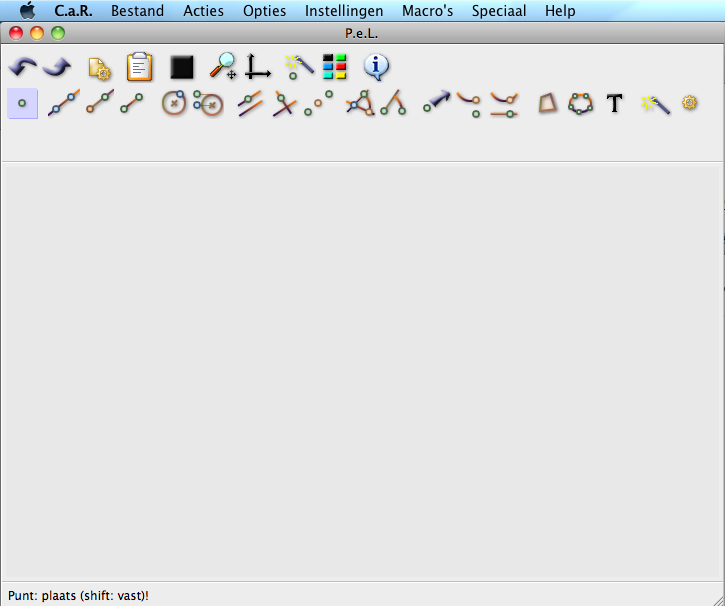
\includegraphics[width=\textwidth]{figuren/PeL/PeLscherm.png}
       \caption{Basisscherm van P.e.L.\ v9.5 met beperkte set werktuigiconen.}
    \label{fig:PeLscherm}
\end{figure}
Je kan vier delen onderscheiden (van boven naar onder\footnote{Het is ook mogelijk om de iconenbalk onder het tekenvenster te zetten. Deze instelling kies je via de opties.}):
\begin{enumerate}
\item Programmamenu's;
\item de iconenbalk;
\item het tekenvenster;
\item de statusbalk.
\end{enumerate}
We merken op dat de iconenbalk een \emph{beperkt aantal iconen} toont. Er zijn er zeker dubbel zoveel. We werken met de `beperkte set werktuigiconen' (aan te vinken in het programmamenu bij `Instellingen'). Je krijgt dan enkel de meest voorkomende iconen te zien. Het is een goed idee om eerst een tijdje te wennen aan de beperkte set iconen en deze dan verder aan te vullen (via `Instellingen') als je vertrouwd bent met het programma. Je kan trouwens alles in P.e.L.\ uitvoeren zonder iconen, via de gewone menu's of via  sneltoetsen (`shortcuts').

Het tekenvenster is de plaats waar de constructie vorm krijgt. Soms kan het nodig zijn om eerst te klikken in dit venster, zodat het \emph{in focus} komt.

De statusbalk is de plaats waar het programma aan de gebruiker laat weten wat het als invoer verwacht \footnote{In de zogenaamde \emph{beschrijvende modus} doet dit vak dienst als invoervak. Meer over deze (snelle) manier van werken vind je op http://wiskunde.khleuven.be}. 

\section{Een voorbeeld}
\subsection{Middelloodlijnen van een driehoek construeren}
We werken stapsgewijs volgende opgave uit: 
\begin{quote}
Construeer de middelloodlijnen van een willekeurige driehoek. 
\end{quote}
Als de constructie klaar is, gaan we op zoek naar een eigenschap van deze drie middelloodlijnen door \'{e}\'{e}n van de punten van de driehoek te verplaatsen.

We gebruiken dit voorbeeld om een aantal principes te illustreren. Een grafisch hoogstaand eindresultaat is iets minder onze bekommernis\footnote{Bij een `echte' constructie moet de grafische kwaliteit \emph{wel} een belangrijk streefdoel zijn. Lijndikte, kleur, benaming, puntsoorten,... kunnen allemaal bijdragen om de constructie zo duidelijk en aantrekkelijk mogelijk te maken.}.

\subsection{Constructie van drie punten}
Alle softwareprogramma's voor dynamische meetkunde hebben met elkaar gemeen dat je eerst een \emph{constructiewerktuig} moet selecteren. Het geselecteerde gereedschap verwacht dan bepaalde invoer van de gebruiker.

Ook punten moet je `construeren'. Kies het puntwerktuig\footnote{We gaan even uit van de veronderstelling dat dit werktuig niet het huidig geselecteerde werktuig is. Het geselecteerde werktuig heeft in de iconenbalk een donkergrijze achtergrond.}. Dat kan op drie manieren:
\begin{enumerate}
\item Klik op het icoon van het puntwerktuig;
\begin{figure}[htb]
    \centering
    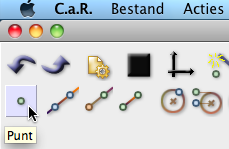
\includegraphics[]{figuren/PeL/Punticoon.png}
       \caption{Selectie via het icoon}
    \label{fig:punticoon}
\end{figure}
\item kies via het menu \texttt{Acties$\rightarrow$Punten$\rightarrow$Punt};
\begin{figure}[htb]
    \centering
    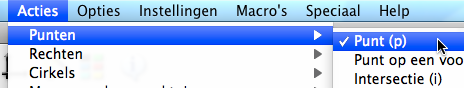
\includegraphics[scale=0.5]{figuren/PeL/Puntmenu.png}
       \caption{Selectie via het menu}
    \label{fig:puntmenu}
\end{figure}
\item De meeste werktuigen hebben een sneltoets. In het menu (zie puntje 2 hierboven) vind je als sneltoets de `p' voor punt\footnote{Meestal is de sneltoets de eerste letter van de Nederlandse benaming van het werktuig, bvb.\ `r' voor rechte, `l' voor lijnstuk, `i' voor intersectie,...}. 
\end{enumerate}
 
Na de selectie staat het icoontje van het puntwerktuig met een donkergrijze achtergrond in de iconenbalk. Het eerste wat je dan doet is de tekst in het statusvenster (onderaan) bekijken. Hier geeft P.e.L.\ aan wat er als invoer verwacht wordt. Bvb.\ in het geval van een punt, staat er `Punt: plaats (Shift: vast)!'. Deze cryptische omschrijving kan je vertalen als: ``Je hebt het puntwerktuig geselecteerd. Ik verwacht nu dat je ergens in het tekenvenster een punt plaatst met de muis. Als je de Shift-toets ingedrukt houdt terwijl je het punt plaatst, maak je een vast punt dat niet meer kan verplaatst worden''. 

Construeer nu drie verschillende punten.

\subsection{Lijnstukken}
Om een driehoek te maken, moet je de drie punten verbinden met lijnstukken. Hiervoor bestaat er een apart werktuig: het \emph{lijnstukwerktuig}. Net zoals bij het puntwerktuig zijn er drie manieren om het te selecteren:
\begin{enumerate}
\item Klik op het icoon van het lijnstukwerktuig;
\begin{figure}[htb]
    \centering
    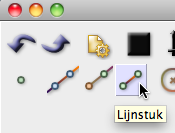
\includegraphics[]{figuren/PeL/Lijnstukicoon.png}
       \caption{Icoon voor lijnstukwerktuig}
    \label{fig:lijnstukicoon}
\end{figure}
\item kies via het menu \texttt{Acties$\rightarrow$Rechten$\rightarrow$Lijnstuk};
\item gebruik de sneltoets `l'. 
\end{enumerate}

Na de selectie van dit werktuig verandert de tekst in het statusvenster in `Lijnstuk: eerste punt?' P.e.L.\ verwacht dat je het eerste punt van het lijnstuk aanduidt. Ga naar \'{e}\'{e}n van de punten met de muis. Als je dicht genoeg in de buurt van het punt met de muisaanwijzer gaat staan, verandert het punt van kleur. Dit betekent dat P.e.L.\ dit punt herkent als een geldige kandidaat. Klik op het punt om het te selecteren. 

Je kan ook klikken op een \emph{vrije ruimte}. P.e.L.\ zal opmerken dat je niet in de buurt van een bestaand punt geklikt hebt en een nieuw punt aanmaken op de plaats waarop je klikte. Opgelet: dit een belangrijke bron van fouten! Meer dan eens gebeurt het dat je denkt op een bestaand punt geklikt te hebben, maar dat je in feite het punt net miste door het onnauwkeurig aan te wijzen.  P.e.L.\ plaatst dan een nieuw punt heel dichtbij het punt dat je eigenlijk wou aanwijzen. Daarom deze raad: \emph{wacht altijd tot het punt dat je wil aanduiden van kleur verandert}. Pas dan ben je zeker dat P.e.L.\ het herkent als een punt dat kan gekozen worden voor het huidige werktuig.

Als alles in orde is verandert de tekst in het statusvak nu in `Lijnstuk: tweede punt (Shift: vaste lengte)?' Vertaling in het Nederlands: ``We werken nog steeds met het lijnstukwerktuig. Duid nu een tweede punt aan als eindpunt voor het lijnstuk. Als je de Shift-toets ingedrukt houdt bij het selecteren van een tweede punt, krijg je een speciaal lijnstuk met vaste grootte''. Op deze voorwerpen met een vaste grootte komen we later terug.

Duid het tweede punt aan (wacht op kleurverandering) en klik met de muis. Het lijnstuk wordt geconstrueerd. Merk op dat de tekst in het statusvak terug verandert naar de tekst van daarnet (eerste punt). \emph{Zolang je geen ander werktuig kiest, blijft het huidige werktuig van kracht}. Construeer nu de andere lijnstukken, tot de driehoek af is.

\subsection{Eigenschappen van een werktuig}
Elk voorwerp dat je construeert wordt bewaard met een aantal standaardeigenschappen, zoals kleur, lijndikte, zichtbaarheid, benaming, grootte,\dots\  Er zijn twee manieren om die eigenschappen te veranderen:
\begin{enumerate}
\item Het gemakkelijkste is dat je \emph{op voorhand} (v\'{o}\'{o}r de constructie van het voorwerp) nadenkt over de gewenste kleur, lijndikte,... en die standaardwaarden aanpast. Deze manier van werken illustreren we in een volgend puntje.
\item Het is echter ook mogelijk om de eigenschappen van een reeds geconstrueerd voorwerp \emph{achteraf} te wijzigen. Ook dit kan op verschillende manieren:
\begin{enumerate}
\item Klik op het icoon van het `wijzigwerktuig' 
\includegraphics[width=0.75cm]{figuren/PeL/wijzigwerktuigicoon.png}. Opgelet: dit icoon krijg je niet te zien in de beperkte set werktuigiconen. Om ook dit icoon te kunnen kiezen, moet je deze instelling eerst uitschakelen. Dit kan via het menu: \\ \texttt{Instellingen$\rightarrow$beperkte set werktuigiconen}.
\item Kies via het menu \texttt{Acties$\rightarrow$Wijzig laatste voorwerp}. Zoals de omschrijving het aangeeft, kan je hiermee \emph{enkel het voorwerp dat je net construeerde}, wijzigen.
\item De snelste manier om de eigenschappen van een voorwerp te wijzigen is rechtsklikken\footnote{Op Mac wordt dat Command (appeltje-toets) + klikken als je maar over \'{e}\'{e}n muisknop beschikt.} op het voorwerp 
\end{enumerate}

\end{enumerate}

Laten we de eigenschappen van een punt bekijken. Klik met de rechtermuisknop op \'{e}\'{e}n van de punten. Er opent een venstertje met een aantal iconen en vakken waarin tekst of getallen ingevuld zijn. Figuur~\ref{fig:punteig} toont dit eigenschappendialoogvenster. Per voorwerp is dit venster licht verschillend (een rechte heeft bvb.\ een paar andere eigenschappen dan een cirkel), maar de basisstructuur is altijd hetzelfde. Daarom bekijken we dit voorbeeld meer in detail.

\begin{figure}[htb]
    \centering
    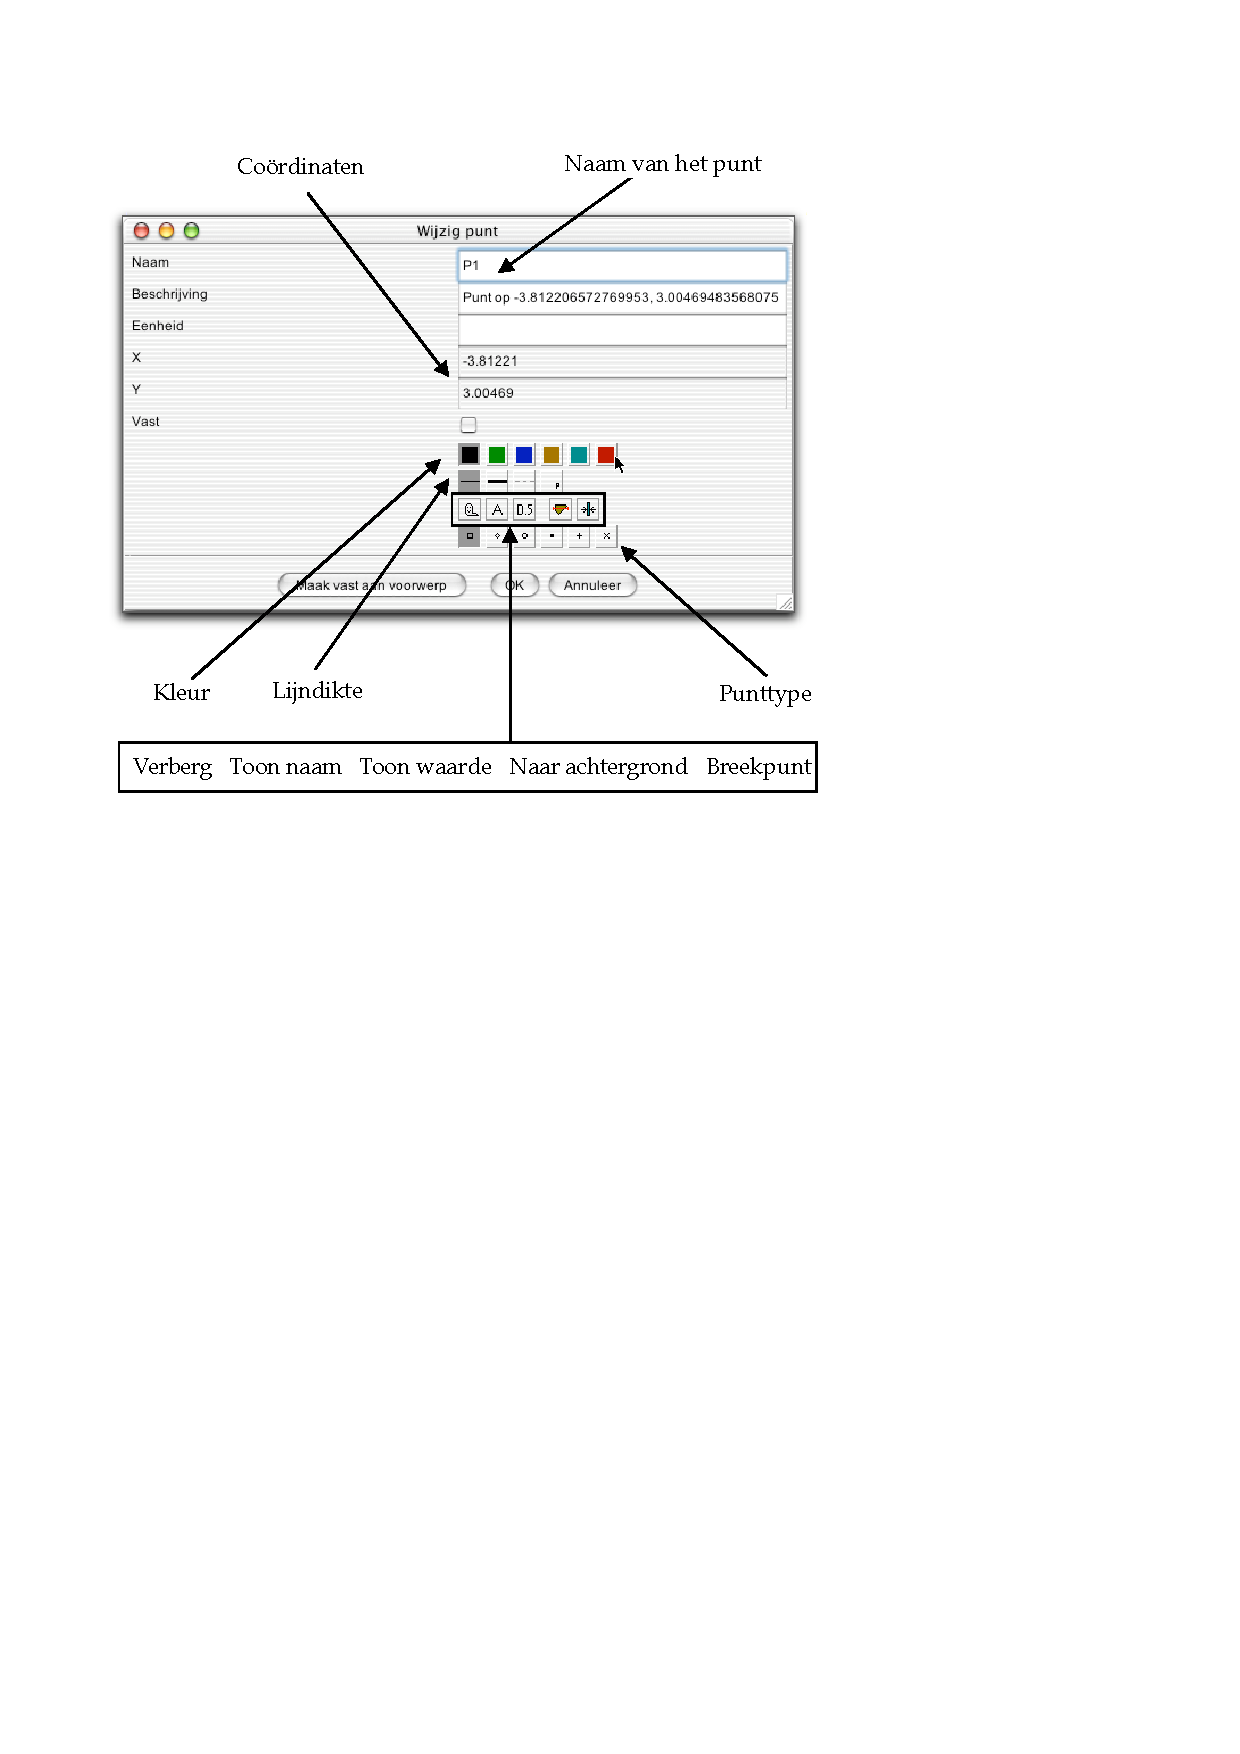
\includegraphics[bb= 42 450 450 780,clip]{figuren/PeL/punteigenschappen.pdf}
       \caption{Eigenschapen van een punt}
    \label{fig:punteig}
\end{figure}

\subsubsection{Benaming -- beschrijving}
P.e.L.\ geeft elk voorwerp een \emph{standaardnaam}. In ons voorbeeld merk je  in het eigenschappenvenster dat punten benoemd worden met een `P' gevolgd door een volgnummer. Bij lijnstukken is dat een `l' met een nummer, snijpunten (intersecties) krijgen  als naam een `I' met een nummer, enz. Voor veel voorwerpen is deze naamgeving prima en is er weinig reden om dat aan te passen.

Voor onze driehoek echter zou het aangenaam zijn als we de `normale' manier van werken zouden kunnen gebruiken: hoekpunten A, B en C. Via het eigenschappendialoogvenster is dat heel simpel. Je klikt in het vakje van de naam en vult de gewenste naam in. Herhaal dit voor de drie punten.

Dit is natuurlijk repetitief werk. Zeker als je de punten van een zeshoek moet benoemen wordt het eentonig. Daarom heeft P.e.L.\ een speciaal commando om dit proces te \emph{automatiseren}: \texttt{Acties$\rightarrow$Hernoem A,B,C} (wat is de sneltoets?).  Het icoon is  niet beschikbaar in de beperkte set werktuigiconen. Je moet deze optie dus uitvinken (\texttt{Instellingen$\rightarrow$Beperkte set werktuigiconen}).
\begin{figure}[htb]
    \centering
    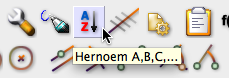
\includegraphics[]{figuren/PeL/herbenoemABC.png}
       \caption{Icoon voor herbenoemen}
    \label{fig:herbenoemicoon}
\end{figure}
Als je dit werktuig kiest, verwacht (zie statusvak!) P.e.L.\ dat je een voorwerp aanklikt. Als je op een punt klikt, zoekt het programma naar de eerste letter die nog niet benomen is, bvb.\ de `A'. Een ander punt aanklikken, levert `B' als benaming, enz. Bij lijnstukken krijg je a, b, c, \dots\ en voor hoeken levert dit $\alpha$, $\beta$, $\gamma$,\dots

Onder de benaming vind je in het dialoogvenster een vak `beschrijving'. Ook hierin komt eens standaardtekst die je kan vervangen door een willekeurige andere tekst. 

\subsubsection{Waarde}
P.e.L.\ laat je blijkbaar toe om vrij in een tekenvenster meetkundige figuren te construeren. Die figuren worden in het programma vertaald in getallen, vergelijkingen, co\"{o}rdinaten. We noemen dit de \emph{waarde} van een voorwerp. Ieder voorwerp heeft zijn specifiek waarde:
\begin{itemize}
\item de waarde van een punt zijn de co\"ordinaten
\item de waarde van een lijnstuk is de lengte
\item de waarde van een cirkel is de  straal
\item de waarde van een hoek is de grootte van de hoek (uitgedrukt in graden)
\end{itemize}
Deze waarde kan je gebruiken in wiskundige uitdrukkingen (\texttt{Acties$\rightarrow$Andere voorwerpen$\rightarrow$Wiskundige uitdrukking}).

 Als je werkt in de permanente instructieweergave (\texttt{Instellingen$\rightarrow$\\Permanente instructieweergave}) kan je de waarde van de voorwerpen gemakkelijk aflezen (zie figuur~\ref{fig:permanent}).
\begin{figure}[htb]
    \centering
    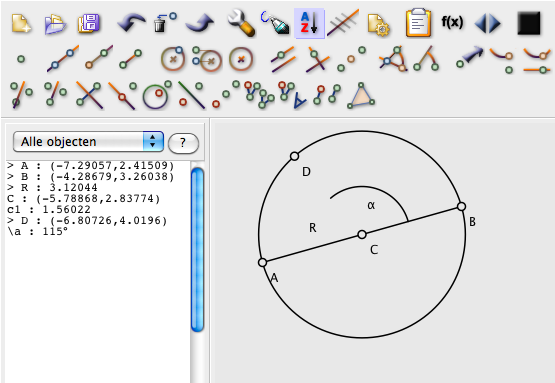
\includegraphics[width=\textwidth]{figuren/PeL/permanente_instructieweergave.png}
       \caption{De permanente instructieweergave}
    \label{fig:permanent}
\end{figure}



\subsubsection{Co\"{o}rdinaten}
Zoals eerder gezegd krijgt elk punt een set van co\"ordinaten. Vaak heb je geen nood aan dit inwendig co\"{o}rdinatensysteem. Voor sommige toepassingen is het wel zinvol dat je met exacte co\"{o}rdinaten werkt. Je kan het raster tonen via het menu \texttt{Opties$\rightarrow$Toon raster} (ga zelf op zoek naar de sneltoets en het bijhorend icoon). Je merkt dat het rastericoon een donkergrijze achtergrond krijgt (met andere woorden: geselecteerd is). Dit is een voorbeeld van een instelling die \emph{voor de hele figuur} van toepassing is (en niet alleen voor een welbepaald voorwerp). 

In het eigenschappenvenster kan je van elk punt de $x$- en de $y$-co\"{o}rdinaat zelf invoeren. Bevestig je keuze en het punt zal opnieuw getekend worden op de co\"{o}rdinaten die je invulde.

Als het raster `aan' staat doen de rasterlijnen dienst als \emph{magneten}. Als je een nieuw punt maakt, wordt dat altijd op een speciale plaats gezet. Experimenteer er maar eens mee. 
In onze constructie brengen de rasterlijnen weinig bij, dus we zetten ze uit. Vooraleer we dat doen, onderzoek je best nog even het effect van de pijltjestoetsen en van de `+' en de `-' toetsen. Soms is een figuur te klein of te groot, of valt ze een stuk buiten het venster. Met deze toetsen kan je de figuur verkleinen of vergroten en verschuiven\footnote{Eigenlijk is dat niet echt correct geformuleerd. De figuur blijft staan, maar het onderliggend co\"{o}rdinatensysteem wordt aangepast. Je kan het ook als volgt bekijken. De constructie wordt op een heel groot blad papier gemaakt. Jij krijgt enkel een klein stuk van dat tekenpapier te zien, door een venster. Dit venster kan je verschuiven over het tekenblad en je kan er een vergrootglas (of verkleinglas) voor zetten.}.

Maar ---\,zoals gezegd\,--- we zetten het rastersysteem af voor de rest van onze constructie.

\subsubsection{Visuele kenmerken}
We gaven het hiervoor al aan. Bepalend voor het eindresultaat is zeker en vast ook een \emph{oordeelkundig gebruik van kleur, puntsoort, lijndikte, naamgeving,...}

In het eigenschappenvenster kan je voor elk voorwerp apart deze eigenschappen instellen. Experimenteer met deze instellingen. Je kan eigenlijk niets fout doen en de meeste dingen zijn voor de hand liggend.

Alleen de `Verberg' optie vraagt een woordje uitleg. Deze mogelijkheid om voorwerpen niet te laten zien op het scherm ---\,ook al zijn ze wel nog aanwezig in de constructie\,--- is absoluut onmisbaar voor meer \emph{complexe constructies}. Tenzij je heel wat tussenstappen onzichtbaar maakt, zie je op den duur door de bomen het bos niet meer. 

Op zich is het een simpele optie. Je duidt bij een voorwerp bij de eigenschappen aan dat het verborgen mag worden. Als je je later zou bedenken, kan je het `verberg' icoontje `uit' zetten. Het probleem is natuurlijk dat je moeilijk een voorwerp kan selecteren (door er rechts op te klikken) dat je niet meer kan zien. De oplossing vind je in het menu: \texttt{Opties$\rightarrow$Toon verborgen voorwerpen} (zoek de sneltoets: bij langere constructies zal je die regelmatig nodig hebben). Net zoals bij het raster is dit ook een optie die voor heel de constructie geldig is, tot je ze uitzet. Verborgen voorwerpen worden in een lichte tint getekend. Je kan nu de eigenschappen van het verborgen voorwerp dat je weer wil tonen, wijzigen (bvb.\ door rechtsklikken). Zet in het eigenschappendialoogvenster de optie `verberg' uit. Je kan nu in het menu \texttt{Opties$\rightarrow$Toon verborgen voorwerpen} terug uitzetten.



\subsection{Midden van de drie zijden}
Na de (toch wel belangrijke) uitwijding hierboven keren we terug naar ons voorbeeld. We hebben al de driehoek getekend en de drie hoekpunten A, B en C genoemd. Deze namen zijn zichtbaar op de constructie. De namen van de lijnstukken worden niet getoond.

Volgende stap: middelloodlijnen tekenen. Er is weliswaar een `middelloodlijn' werktuig\footnote{Perpendicular Bisector 
\includegraphics[width=0.75cm]{figuren/PeL/middelloodlijnicoon.png}}, maar daar gaan we geen gebruik van maken. We werken daarom in twee stappen en zoeken eerst de middens van de zijden. 

Het verhaal ken je stilaan. Je selecteert het `midden' werktuig (via het menu, via een icoon of via een sneltoets) en werpt een blik op het statusvak linksonder. Als daarin de tekst `Middelpunt: eerste punt?' verschijnt, zit je goed. 

Dit keer proberen we slim te zijn. \emph{Vooraleer} de middens te construeren, denken we even na hoe we die getoond willen zien. Nemen we bvb.\ dat we ze in het rood, met een bolletje en voorzien van de standaardbenaming willen tonen. Hierboven zag je reeds hoe je na de constructie nog eigenschappen kan veranderen. Als je echter op voorhand weet wat je wil, is het effici\"{e}nter om het op voorhand te bepalen. 

In wat volgt werken we via het menu. Ook hier kan je de selectie via de iconen doen. Denk er wel aan dat deze instellingen blijven gelden voor alle voorwerpen die je vanaf nu construeert. Kies in het menu achtereenvolgens volgende instellingen:
\begin{itemize}
\item \texttt{Opties$\rightarrow$Standaard kleur$\rightarrow$rood}
\item \texttt{Opties$\rightarrow$Standaard punttype$\rightarrow$Cirkel}
\item \texttt{Opties$\rightarrow$Voorkeuren$\rightarrow$Toon voorwerpnamen}
\end{itemize}
De andere instellingen laten we zoals het is. Merk je in de iconenbalk wat er veranderd is? Construeer nu de middens van de drie zijden.

\subsection{Loodlijnen}
We willen de drie loodlijnen graag in een blauwe stippellijn tekenen. De namen willen we er liever niet bij. Pas de opties in die zin aan. Zoek zelf het loodlijn gereedschap. Kijk in de statusbalk wat P.e.L.\ van jou verwacht. De volgorde van de invoer is belangrijk: moet je eerst de rechte aanduiden en dan het punt of is het omgekeerd? 


\section{Opbouw van een constructie}
Het boeiende aan programma's zoals P.e.L.\ is dat je de zogenaamde \emph{vrije punten} van de constructie kan verplaatsen. De tekening past zich dan aan aan de nieuwe situatie. We noemen dit het \emph{dynamisch} of het \emph{interactief} karakter van dit soort van meetkundeprogramma's. 

In P.e.L.\ kan je \emph{enkel punten} verplaatsen. Het verschil tussen vrije en niet-vrije punten is in dit opzicht belangrijk. In ons voorbeeld zijn de drie hoekpunten van de driehoek vrije punten. Het zijn punten die we willekeurig ergens in het tekenvenster geplaatst hebben\footnote{Hadden we de Shift-toets ingedrukt gehouden bij het cre\"{e}ren van de punten, dan waren dit vaste punten geweest.}. Een vrij punt kan je met het `beweeg' werktuig verplaatsen. Dit werktuig kan je op de gebruikelijke manieren selecteren, bvb.\ via de sneltoets `b' (zoek zelf hoe je het doet met een icoon of via het menu!). Als je dit werktuig geselecteerd hebt, krijg je feedback van het programma via de statusbalk en via het tekenvenster. Alle vrije (beweegbare) punten worden immers \emph{rood gekleurd} en in het \emph{vet} weergegeven. Klik op zo'n punt, hou de muisknop ingedrukt en verplaats het punt. De hele constructie past zich aan. Tip: \emph{als je de Ctrl-toets ingedrukt houdt, blijf je de originele tekening zien}.

De middelpunten van de zijden zijn \emph{geen} vrije punten. Hun plaats ligt vast, want ze volgt uit een berekening waar twee vrije punten de invoerparameters zijn. 

Tijdens de constructie maak je onvermijdelijk ooit wel eens een \emph{fout}. Als je het laatst geconstrueerde voorwerp wil wissen is het vrij eenvoudig: \texttt{Acties$\rightarrow$ Wis laatste voorwerp}. Onthoud misschien best ook de sneltoets voor deze bewerking. Je zal immers regelmatig wel eens iets moeten wissen.

Als je \emph{pas na een aantal stappen} merkt dat je in het begin een fout maakte, wordt het iets moeiljker. Je gebruikt hiervoor \texttt{Acties$\rightarrow$Verwijder voorwerp en zijn kinderen}. De klemtoon bij deze actie ligt echt wel op `en zijn kinderen'. Als je in onze driehoek \'{e}\'{e}n van de hoekpunten verwijdert, valt een groot deel van de constructie mee weg (ga eens na wat er allemaal van dit ene punt afhangt). Kalm blijven is de boodschap! Denk eerst eens goed na of je wel het goede voorwerp wil wissen. Als het dan toch fout loopt (en je bent een groot deel van je constructie kwijt) is `\texttt{Acties$\rightarrow$Maak wissen ongedaan' (Ctrl-Z)} je bondgenoot. \emph{Voorwaarde is wel dat je na je fatale wisbewerking geen andere bewerkingen meer deed}. 

Zoals bij elk computerprogramma neem je natuurlijk je voorzorgen en bewaar je je werk regelmatig. 

\section{De omcirkel}
Hoe je ook de driehoek aanpast (door punten te verplaatsen), de middelloodlijnen op de drie zijden gaan altijd door \'{e}\'{e}n punt. Dit snijpunt ligt even ver van de drie hoekpunten verwijderd. We kunnen met andere woorden een cirkel tekenen die door de drie hoekpunten van de gegeven driehoek gaat, met als middelpunt het snijpunt van de middelloodlijnen.

\emph{Werken met snijpunten} is anders in dit soort van programma's dan bij een constructie op papier. Als je op papier twee snijdende rechten tekent met een potlood, heb je automatisch een snijpunt. Bij programma's voor dynamische meetkunde moet je dit snijpunt meestal expliciet aangeven, vooraleer je het kan gebruiken\footnote{Dit is een vereenvoudiging van hoe je in P.e.L.\ werkt. Het kan ook zonder dit punt expliciet te benoemen, maar we leggen hier de standaardmanier van werken uit}. Om snijpunten te construeren beschik je over een apart gereedschap: het `intersectie' werktuig.

Kies dit werktuig. In de statusbalk merk je dat er verschillende mogelijkheden zijn om het snijpunt te construeren:
\begin{enumerate}
\item Je kan de verschillende snijdende voorwerpen \'{e}\'{e}n voor \'{e}\'{e}n selecteren.
\item Je kan echter ook rechtstreeks op het snijpunt klikken. Soms is dit niet mogelijk omdat je bvb.\ \emph{alle} snijpunten wilt (bvb.\ tussen een rechte en een cirkel) of omdat het snijpunt heel dicht bij andere punten ligt.
\end{enumerate}
Hier kan je kiezen welke methode je gebruikt. Construeer het snijpunt.

Om een cirkel te construeren zijn er verschillende mogelijkheden:
\begin{itemize}
\item Cirkel met gegeven middelpunt en een punt op de cirkel;
\item cirkel met gegeven middelpunt  en nog twee andere punten die de straal bepalen;
\item cirkel met gegeven middelpunt en een in te voeren lengte als straal.
\end{itemize}
De keuze hangt af van de omstandigheden. Voor deze constructie ligt de eerste optie voor de hand. De statusbalk helpt je wel verder bij de juiste keuze van de punten (eerst het middelpunt selecteren, en dan \'{e}\'{e}n van de hoekpunten van de driehoek).


\section{Constructievoorbeelden stap voor stap}
\subsection{Vierkant}
\begin{quote}
Teken een vierkant $ABCD$ met een willekeurige zijde.
\end{quote}
\begin{figure}
\begin{center}
\setlength{\fboxrule}{0.4pt}
\setlength{\fboxsep}{0.1pt}
\framebox{
\setlength{\unitlength}{0.008466666666666667cm}
\begin{picture}(1181.0,708.0)
\put(0,0){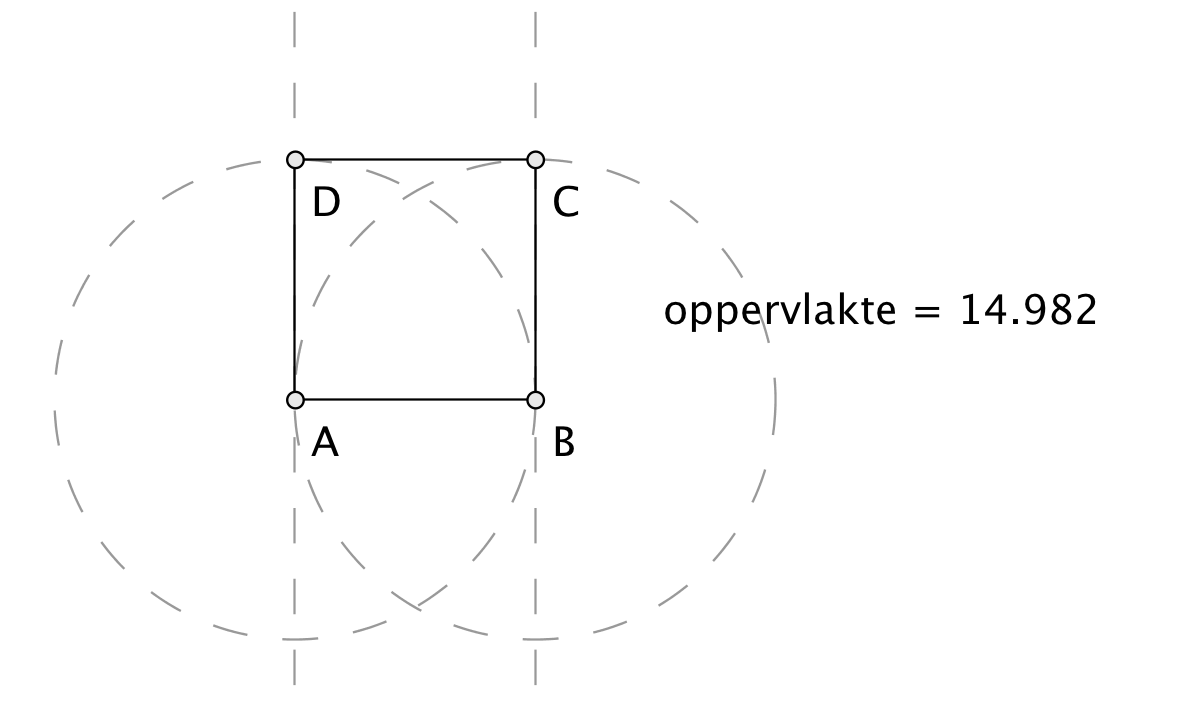
\includegraphics[width=9.999cm]{figuren/PeL/vierkant.png}}
\put(403.072,343.191){$a$}
\put(243.646,413.511){$d$}
\put(404.072,583.438){$c$}
\put(560.499,413.511){$b$}
\end{picture}
}
\end{center}
\caption{Constructie van een vierkant}
\label{fig:vierk}
\end{figure}
\begin{enumerate}
\item Teken de punten $A$ en $B$. Gebruik het werktuig \knop{Hernoem A,B,C} om de punten de correcte naam te geven.
\item Verbind beide punten met een lijnstuk. Benoem het lijnstuk $a$.
\item Construeer nu de rechteropstaande zijde als volgt:
\begin{enumerate}
\item Maak een loodrechte op $a$ door het punt $B$ in stippellijn.
\item Teken in stippellijn een cirkel met middelpunt $B$ en straal gelijk aan de lengte van $a$. Je gebruikt daarvoor het werktuig \knop{Cirkel met straal r en middelpunt M}. Volg de instructies van de instructiebalk nauwkeurig op. Het beginpunt van de straal is het punt $A$ en het eindpunt $B$.
\item Bepaal het snijpunt van de cirkel en de loodrechte met het werktuig \knop{Intersectie}. Verander eerst de lijndikte.
\item Benoem het bovenste snijpunt $C$ en verwijder het andere snijpunt met \knop{Verwijder voorwerp en zijn kinderen}.
\item Teken het lijnstuk $BC$. Benoem de zijde $b$.
\end{enumerate}
\item Construeer nu de linkeropstaande zijde $AD$ op dezelfde manier als $BC$ en benoem hem $d$.
\item Teken het lijnstuk $CD$ en noem het $c$.
\end{enumerate}

Je hebt nu het vierkant $ABCD$ getekend. Je kan de lengte van de zijde van het vierkant wijzigen door de punten $A$ of $B$ te slepen met het werktuig \knop{Beweeg punt}. Merk op dat de punten $C$ en $D$ niet vastgenomen (om ze te verslepen) kunnen worden. Zij zijn immers {\it vaste punten}: ze zijn het resultaat van een aantal bewerkingen.

De tekening wordt eleganter als je de hulplijnen verbergt (niet verwijderen!). Je kan ze op de achtergrond zichtbaar maken met \knop{Toon verborgen voorwerpen}.

Bewaar je afbeelding. Verwijder dan het punt $A$. Wat merk je? Zoek een verklaring.

Veronderstel dat we ook de oppervlakte van het vierkant willen tonen op het scherm. Daarvoor gebruiken we het  werktuig \knop{Wiskundige uitdrukking}. Als je op de knop klikt, krijg je het dialoogvenster zoals in figuur~\ref{fig:wisk_uitdr}.
\begin{figure}
\centering
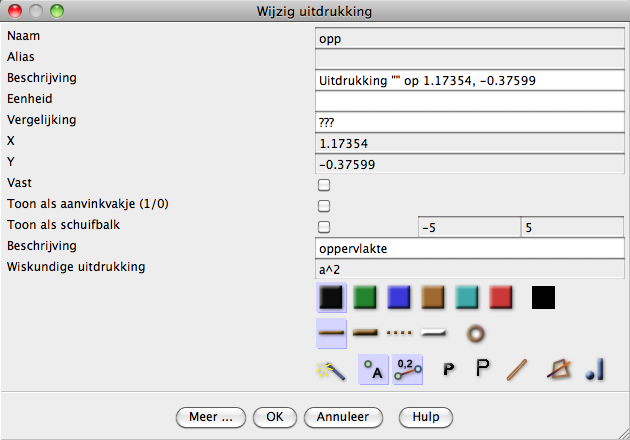
\includegraphics[width=\textwidth]{figuren/PeL/wisk_uitdrukking.png}
\caption{Dialoogvenster van het werktuig `Wiskundige uitdrukking'}
\label{fig:wisk_uitdr}
\end{figure}
\begin{enumerate}
\item Een wiskundige uitdrukking is een voorwerp, net zoals een cirkel, en heeft dus een naam en een waarde. Met de naam (hier `opp') kan je de waarde oproepen in een ander voorwerp (bijvoorbeeld bij een cirkel met vaste straal). 
\item Vul het onderste veld \knop{Beschrijving} in met \veld{oppervlakte}.  Deze tekst verschijnt bij de tekening (zie afbeelding~\ref{fig:vierk}). 
\item Bij \knop{Wiskundige uitdrukking} vul je de waarde in die je wil bekomen, namelijk het kwadraat van het lijnstuk $a$. Je kan dit doen op twee manieren: ofwel vul je gewoon \verb/a^2/ in (de waarde van het lijnstuk $a$ is immers zijn lengte), ofwel gebruik je de functie \veld{d(A,B)} waarbij je de afstand tussen de punten $A$ en $B$ berekent. \item Vink zowel \knop{Toon voorwerpnamen} als \knop{Toon voorwerpwaarden} aan.
\end{enumerate}
Met het werktuig \knop{Wiskundige uitdrukking} kan je ook een voorwerp maken waarvan de waarde bepaald wordt door middel van een schuifbalk. Je vult het veld `Wiskundige uitdrukking' niet in, maar je vinkt het vakje 'Toon als schuifbalk' aan. In de figuur verschijnt dan een schuifbalk. Door het punt op de schuifbalk te verschuiven, wijzig je de waarde van het voorwerp.

\subsection{Lindenmayer-fractaal}
De Lindenmayer-fractaal ziet er als volgt uit:
\begin{center}
\setlength{\fboxrule}{1.pt}
\setlength{\fboxsep}{0.1pt}
\scalebox{0.4}{\framebox{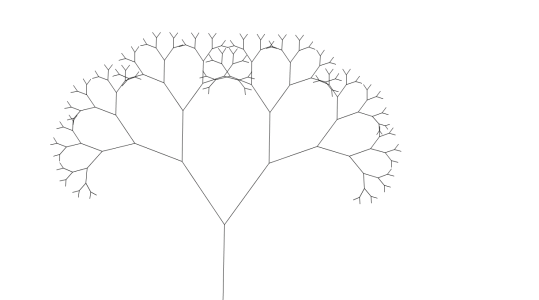
\includegraphics{figuren/PeL/lindmayer.png}}}
\end{center}

Ze wordt iteratief opgebouwd. Dit wil zeggen: je vertrekt van een stam en daar teken je twee takken op. Vervolgens beschouw je elk van deze takken opnieuw als stam en teken je telkens twee (kleinere) takken. De verhouding van de lengte tak - onderliggende tak moet telkens gelijk zijn.
\begin{center}
\setlength{\fboxrule}{1.pt}
\setlength{\fboxsep}{0.1pt}
\scalebox{0.5}
{\framebox{
\setlength{\unitlength}{0.008466666666666667cm}
\begin{picture}(1417.0,929.0)
\put(0,0){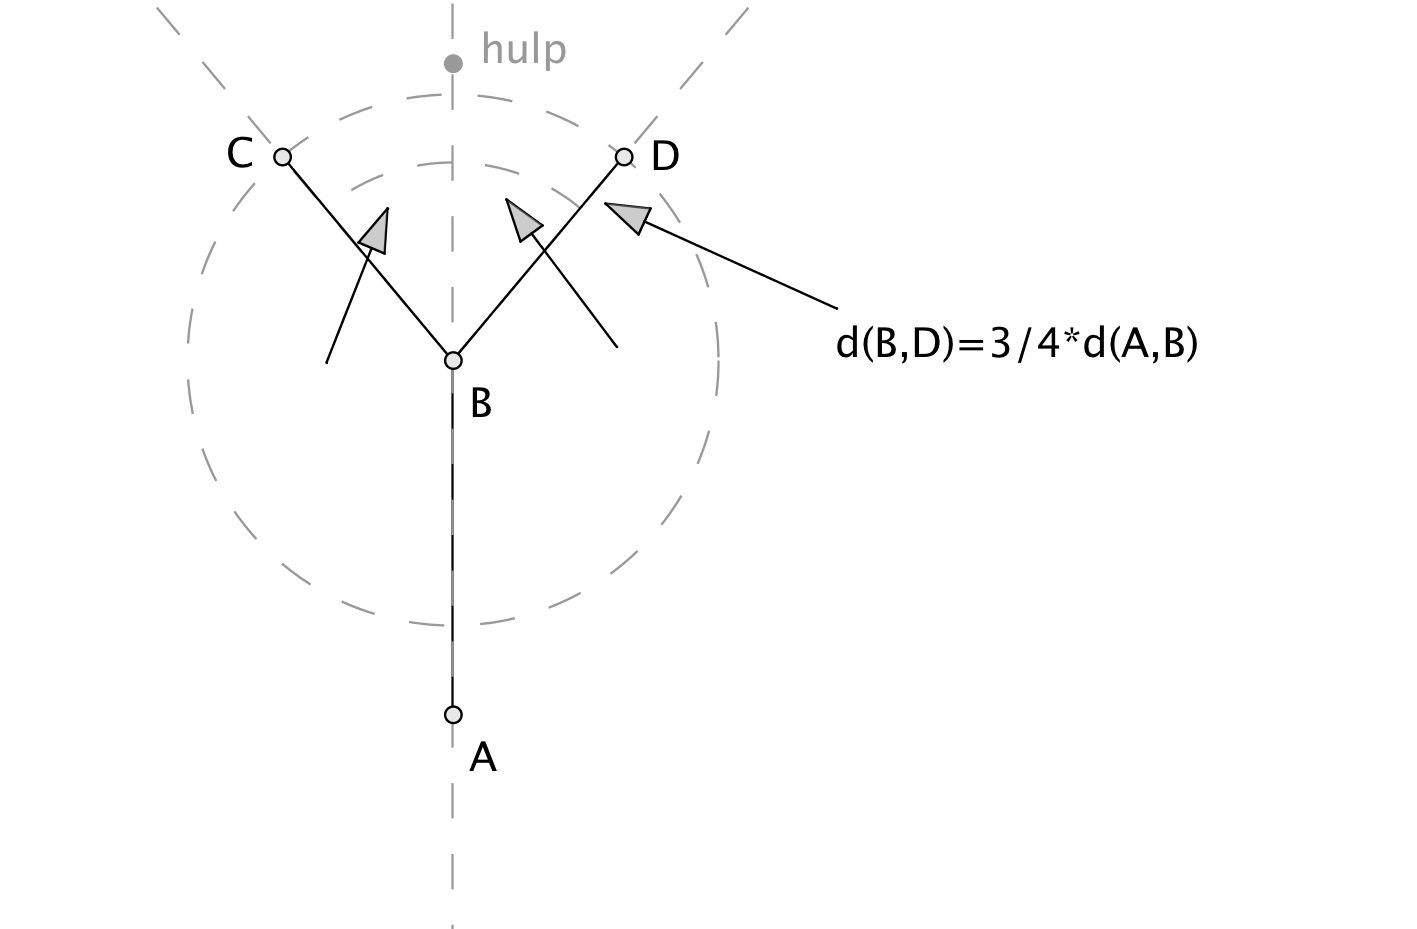
\includegraphics[width=11.997cm]{figuren/PeL/flower.png}}
\put(390.07,121.222){$r_1$}
\put(245.424,516.593){$\alpha=40^\circ$}
\put(576.436,527.929){$\beta=40^\circ$}
\end{picture}
}}
\end{center}
De constructie is wat moeilijker en maakt gebruik van macro's. We beginnen met het tekenen van een stam en zijn twee takken.

\begin{enumerate}
\item Construeer het \knop{lijnstuk} $a$ van $A$ tot $B$.
\item Maak in stippellijn de \knop{rechte} $r_1$ door $A$ en $B$.
\item Definieer een \knop{punt} \veld{hulp} op deze rechte, ten noorden van $B$.
\item Construeer de \knop{vaste hoeken} $\alpha$ en $\beta$ van $40^\circ$ met \knop{beginpunt} \veld{hulp} en \knop{basispunt} $B$\footnote{Let op de volgorde! Indien je straks problemen hebt bij de macro, kom dan terug naar deze stap.}. \label{voetnoot_lindmayer}
\item Construeer in stippellijn de \knop{cirkel} $c_1$ \knop{met vaste straal}  \veld{3/4*d(A,B)} en middelpunt $B$.
\item Bepaal de snijpunten $C$ en $D$ van deze cirkel met de hoeken $\alpha$ en $\beta$ respectievelijk.
\item Teken de lijnstukken $BC$ en $BD$. Deze lijnstukken zijn de takken op de stam $AB$.
\end{enumerate}

In feite heb je nu de eerste iteratie van de fractaal getekend. Een fractaal met \'e\'en iteratie is echter geen fractaal. Op {\it beide} takken die je getekend hebt, zou je nu opnieuw de ganse constructie moeten hernemen. Dit geeft vier (kleinere) takken, waarop je opnieuw takken moet maken \dots\ Het zal een werk van zeer lange adem zijn.

Het is bijgevolg beter een {\it macro} te maken. Een macro is in feite een samenraapsel van een aantal opeenvolgende constructies. Eens hij gedefinieerd is, volstaat het \'e\'en of meerdere beginpunten of -voorwerpen ({\knop{parametervoorwerpen}) aan te duiden. De macro zorgt er dan voor dat het eindresultaat (\knop{doelvoorwerpen}) getekend worden.

We maken nu de macro {\tt lindenmayer} die de stam $AB$ als {\knop{parametervoorwerp} heeft en de takken $BC$ en $BD$ als \knop{doelvoorwerpen}. We gebruiken hiertoe bovenstaande constructie.

\begin{enumerate}
\item Klik op de knop \knop{Macro parameters/doelen/definitie}.
\item P.e.L.\ vraagt \knop{Macro parameters: parametervoorwerpen?}. Dit zijn de gegevens waarop het uiteindelijke resultaat van je macro gebaseerd zijn. Hier heb je twee mogelijkheden: je zou de punten $A$ en $B$ kunnen aanklikken, maar ook het lijnstuk $AB$ (dat op deze punten gedefinieerd is). Wij kiezen voor de laatste mogelijkheid.
\item \label{lindmayer: stap 3} Klik opnieuw op de knop \knop{Macro parameters/doelen/definitie}. Merk op dat de knop verandert, en dat een deel van de constructie verdwijnt\footnote{Dit is niet abnormaal. Indien echter de takken $BC$ en $BD$ ook verdwijnen, heb je de constructie verkeerd gemaakt. Lees opnieuw de voetnoot op blz.~\pageref{voetnoot_lindmayer}.}. P.e.L.\ vraagt nu \knop{Macro doelen: doelvoorwerpen?}. Wat moet het resultaat zijn van je macro? Wij willen dat de macro twee takken op de stam $AB$ tekent, dus we klikken de lijnstukken $BC$ en $BD$ aan.
\item Klik een laatste keer op de knop \knop{Macro parameters/doelen/definitie}. P.e.L.\ vraagt je nu de \knop{naam} van de macro te specifi\"eren. Verder kan je de macro van commentaar voorzien en in het veld \knop{Vraag naar parameters} een zinvolle naam invullen (bijvoorbeeld \veld{stam} in plaats van het standaard voorziene $l_1$).
\item Klik op OK en je macro is klaar.
\end{enumerate}

Misschien lukte bovenstaande procedure niet omdat in stap~\ref{lindmayer: stap 3} je scherm opeens leeg was. De oorzaak hiervan ligt in een foute constructievolgorde. De doelvoorwerpen moeten {\it volledig} afhankelijk zijn van de parametervoorwerpen. Je mag bijvoorbeeld de hoek van $40^\circ$ niet defini\"eren op een rechte die niet door $A$ en $B$ gaat (maar wel door twee andere punten op het lijnstuk $AB$). Op zicht zal je dezelfde takken krijgen, maar voor P.e.L.\ maakt het een groot verschil: de takken zijn immers afhankelijk van de nieuwe punten, en niet van $A$ en $B$. V\'o\'or je een macro begint zou je de volgende test moeten doen: verwijder de parametervoorwerpen\footnote{Eerst constructie opslaan!}. Indien de doelvoorwerpen niet verdwijnen, is de constructievolgorde fout en zal je ook geen macro kunnen defini\"eren.

Nu je de macro gemaakt hebt, kan je hem gebruiken.
\begin{enumerate}
\item Klik rechts op het scherm en selecteer de macro.
\item P.e.L.\ vraagt je naar het parametervoorwerp \veld{stam}. Klik op een tak waar je zijtakken wil.
\item De zijtakken worden getekend.
\end{enumerate}
Het kan zijn dat je een foutief resultaat krijgt, bijvoorbeeld dat de nieuwe takken naar beneden wijzen in plaats van naar boven. Dit is opnieuw te wijten aan een foute constructievolgorde (bijvoorbeeld het lijnstuk $AB$ construeren van $B$ naar $A$ in plaats van $A$ naar $B$. Er is maar \'e\'en oplossing: opnieuw beginnen met de volledige constructie en nu de juiste volgorde aanhouden.


 
% 2012/09/10 [Greetje] Enkele opmerkingen toegevoegd nav versie 5.4; enkele oefeningen over grafieken toegevoegd
% 2012/09/06 [Greetje] label toegevoegd voor hoofdstuk
% 19/02/2012 [Jan]: Oefeningen hernummerd met begin{oef} enz. Tabellen iets opgefrist, fouten 
%verbeterd

\chapter{Beknopte handleiding Scilab}
\label{scilab}
\begin{quote}
     \textit{{\small `Ik heb de das gekregen', vervolgde Wiggel 
Waggel nadenkend, terwijl hij de ene knie over de andere sloeg en 
zijn handen eromheen vouwde, `ik heb hem gekregen ---als 
onverjaardagscadeau'}}

     \textit{{\small `Pardon?' zei Alice met een verbluft gezicht.}}

     \textit{{\small `Ik ben niet beledigd,' zei Wiggel Waggel.}}

     \textit{{\small `Ik bedoel, wat is een onverjaardagscadeau?'}}
     \textit{{\small `Een cadeau gegeven wanneer het niet je verjaardag is, natuurlijk.'}}
	\textit{{\small Alice dacht even na. `Ik hou het meest van verjaardagscadeaus,' zei ze tenslotte.}}
	
	
\textit{{\small `Je weet niet waar je het over hebt!' riep wiggel 
Waggel. `Hoeveel dagen zitten er in een jaar?'}}
	
	\textit{{\small 
`Driehonderdvijfenzestig,' zei Alice.}}
			
	\textit{{\small `En 
hoeveel verjaardagen heb je?'}}
	
	\textit{{\small `E\'{e}n.'}}
	
	
\textit{{\small `En als je \'{e}\'{e}n aftrekt van 
driehonderdvijfenzestig, wat blijft er dan over?'}}
	
	
\textit{{\small `Driehonderdvierenzestig natuurlijk.'}}
	
		
\textit{{\small Wiggel Waggel leek te weifelen. `Dat zie ik liever 
even op papier,' zei hij.}}
		
          Uit `Achter de spiegel' -- Lewis Carroll
\end{quote}

\newpage

\section{Inleiding}

Het (freeware-)pakket Scilab\footnote{Download en documentatie op www.scilab.org.} is geschikt om numerieke problemen op te lossen. Het beschikt daarvoor over een omvangrijke ingebouwde functieset. Je kan deze set uitbreiden en aanpassen aan je eigen behoeften door gebruik te maken van de programmeermogelijkheid die Scilab biedt.

De aangewezen  manier om te leren programmeren in Scilab is experimenteren en voorbeelden bekijken (\texttt{.sci} en \texttt{.sce} bestanden).

Op \url{http://www.scilab.org/support/documentation/} vind je volledige documentatie. In het bijzonder raden we de documentatie onder het item `Tutorials' aan.  Verder heeft Scilab een goed uitgebouwde helpfunctie. Typ \verb+help+ in de commandolijn en het helpvenster verschijnt.


\section{De werkomgeving}
De werkomgeving van Scilab (vanaf versie 5.2) bestaat uit verschillende vensters:
\begin{itemize}
\item de `console' waar je bewerkingen kan uitvoeren;
\item een `editor' waar je programma's kan schrijven;
\item grafische vensters waar grafieken getoond worden;
\item het help-venster.
\end{itemize}
In Scilab 5.4 komen er nog vensters bij:
\begin{itemize}
\item een `file browser' om gemakkelijk bestanden terug te vinden
\item een `variable browser' waar je kan aflezen welke veranderlijken je reeds definieerde
\item de `command history' waar de opeenvolgende commando's die je uitvoerde opgelijst worden.
\end{itemize}


\subsection{De console}
Als je Scilab opent, verschijnt het consolevenster (figuur \ref{fig:console}).

\begin{figure}[h!t]
   \begin{center}
    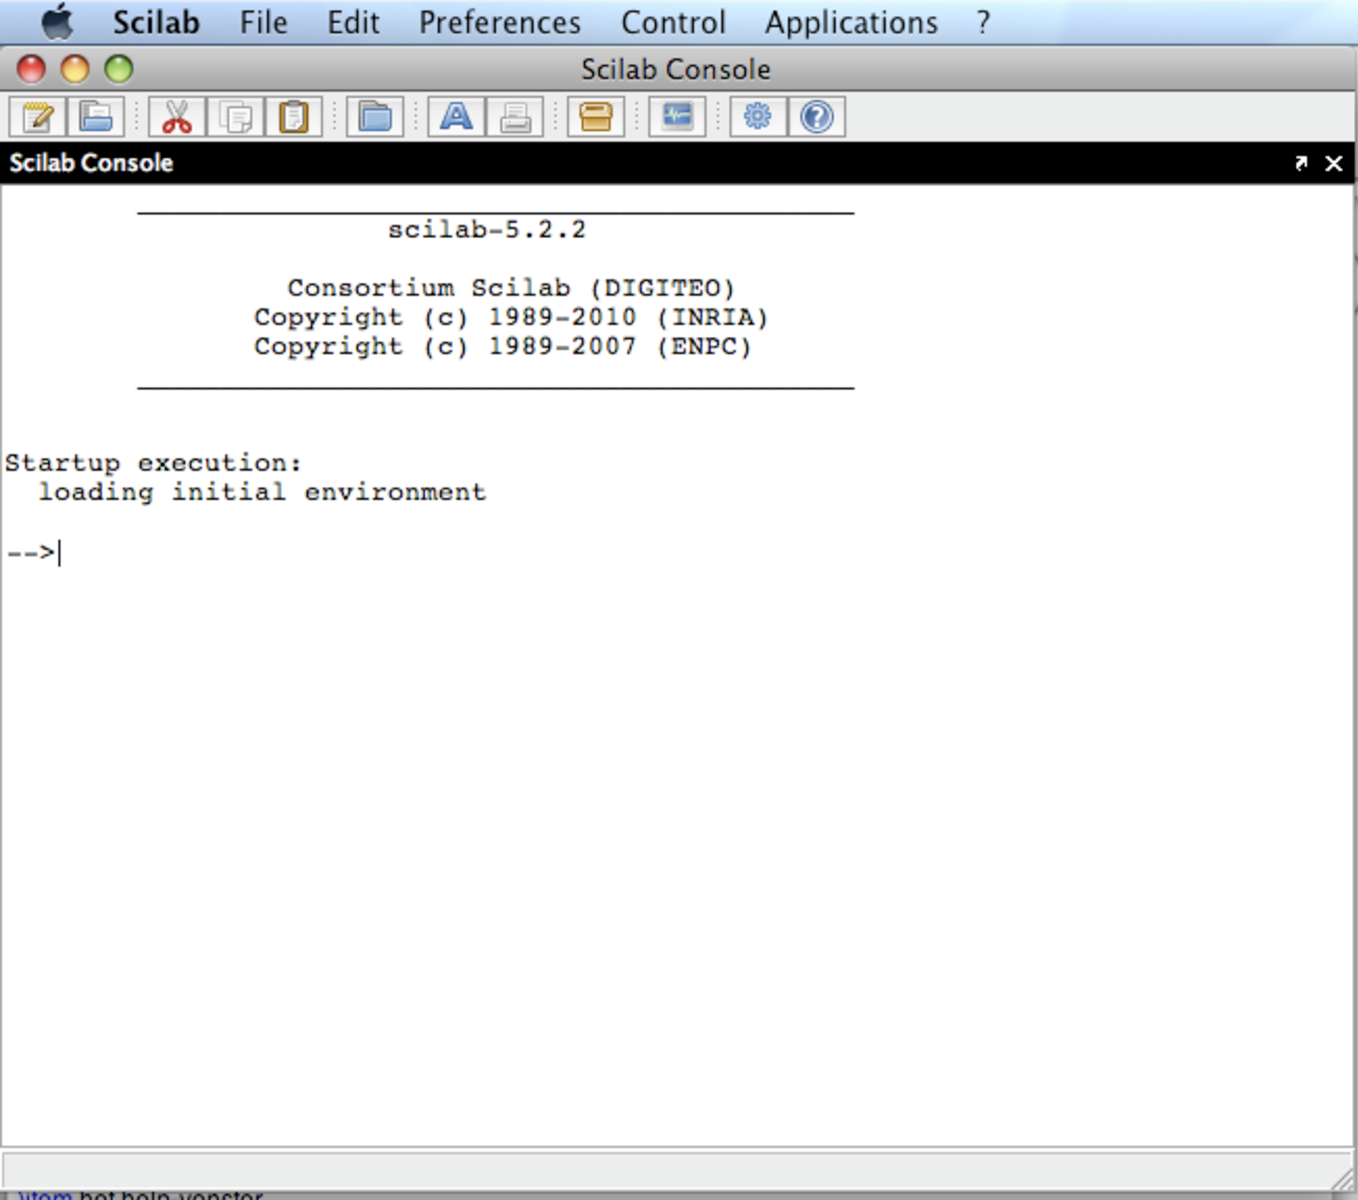
\includegraphics[width=\textwidth, trim= 0cm 10cm 0cm 0cm, clip]{figuren/scilab/01console}
  \caption{Console van Scilab}
	\label{fig:console}
	\end{center}
\end{figure}

Instructies worden ingevoerd na de prompt (\verb+-->+) via het toetsenbord en worden uitgevoerd door de return-toets in te drukken. Een vorige regel kan je laten uitvoeren door met de pijltjestoetsen te werken. Het console venster kan je leegmaken met de toets \verb+F2+.

\subsection{Rekenen met getallen}

Het programma kent de bewerkingen \verb0+0, \verb+-+, \verb+*+, \verb0/0 en voor de machtsverheffing \verb+^+. Als de exponent uit meerdere termen bestaat, dan plaatsen we die tussen haakjes.
Het decimaal punt wordt met een punt genoteerd (en geen komma).  Meerdere instructies worden van elkaar gescheiden d.m.v.\ een komma. Output wordt onderdrukt door gebruik te maken van de puntkomma ';'.


\begin{lstlisting}[caption={Eenvoudige bewerkingen}, label={eenvoudigebewerkingen}]
-->4+5.5
  ans =

     9.5

-->3*4^2-10,-1^2*3+7,(-1)^(2*3)+7
  ans =
	
     38.
  ans =

     4.
  ans =
     8.
-->sqrt(25)+6;
 
-->
\end{lstlisting}

Scilab is hoofdlettergevoelig. Bijvoorbeeld voor de vierkantswortel:


\begin{lstlisting}[caption={Vierkantswortel}, label={vierkantswortel}]
-->sqrt(25), sqrt(368)
 ans  =
 
    5.  
 ans  =
 
    19.183326
    
-->SQRT(9)
        !--error 4 
Undefined variable: SQRT     
\end{lstlisting}


Constanten zoals $\pi$, $e$, t (true) en f (false) worden voorafgegaan door \%.

\begin{lstlisting}[caption={Constanten}, label=constanten]
-->%pi,%e 
 %pi  =
 
    3.1415927  
 %e  =
 
    2.7182818  
 \end{lstlisting}


Scilab heeft een aantal ingebouwde functies zoals \verb+log()+, \verb+abs()+, \verb+ceil()+,\\ \verb+floor()+, \verb+modulo(n,m)+, \verb+sin()+, \verb+cos()+ \ldots\ Je kan de tab-toets gebruiken om de naam van een functie aan te vullen als je slechts de eerste letters van de functienaam weet (figuur \ref{fig:tabtoets}). Merk op dat --\,in tegenstelling tot de gangbare rekenmachines\,-- de functie \verb/log()/ de logaritmische functie is met grondtal \verb/e=2.7182818/ en niet met grondtal 10.

\begin{lstlisting}[caption={Enkele ingebouwde functies}, label=ingebouwdefuncties]
-->abs(-5),floor(6.3),log(30),modulo(25,3)
  ans =

     5.
   ans =

     6.
  ans =

     3.4011974
  ans =

     1.
\end{lstlisting}

\begin{figure}[h!t]
   \begin{center}
    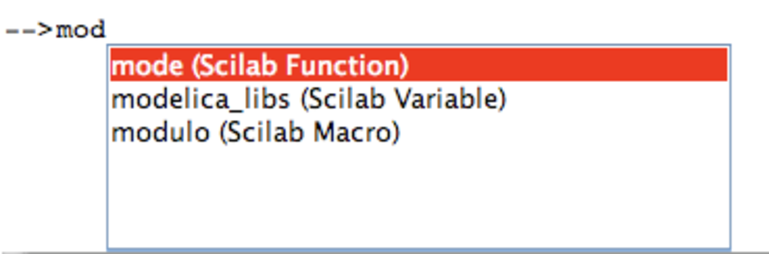
\includegraphics[width=0.8\textwidth]{figuren/scilab/02tabtoets}
  \caption{Gebruik de tabtoets als je een functienaam niet meer volledig weet.}
	\label{fig:tabtoets}
	\end{center}
\end{figure}

\newpage
\subsection{De editor}

Rechtstreeks werken in de console heeft een belangrijk aantal beperkingen: als je een bewerking over meerdere lijnen schrijft, kan je de vorige lijnen niet meer corrigeren. Vanaf versie 5.4 kan je weliswaar een sessie  opslaan(`save environment'), maar het is niet zo handig.  Het is daarom beter om de editor te gebruiken. Je opent het venster als je klikt op het eerste icoontje in de toolbar van de console of via de menubalk: Applications - SciNotes.

In de editor kan je meerdere bewerkingen op dezelfde lijn zetten. Je moet ze dan scheiden met een komma of puntkomma. Dit komt de leesbaarheid wel niet ten goede. Je kan de code documenteren door een lijn te beginnen met \verb+//+. 

\begin{figure}[h!t]
   \begin{center}
    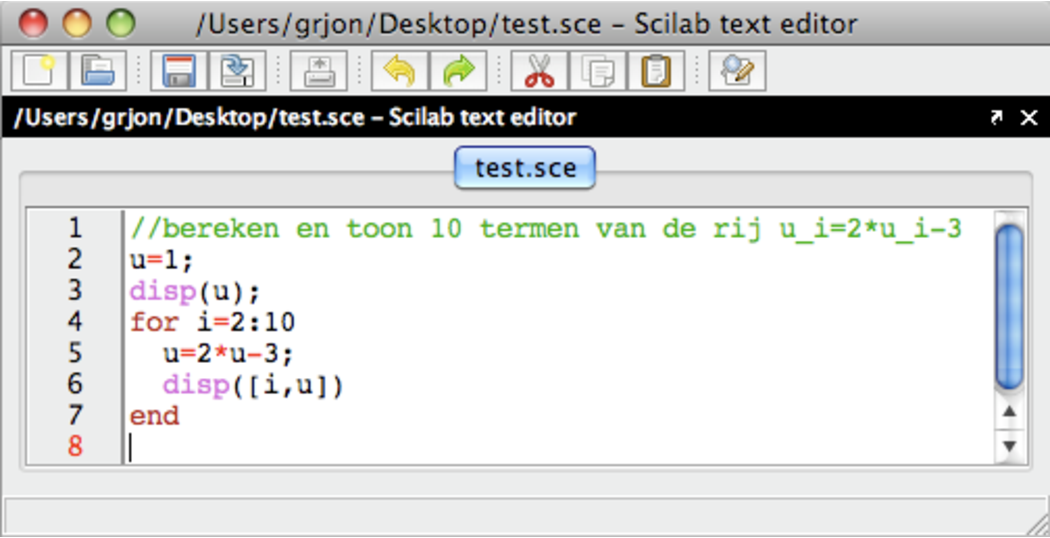
\includegraphics[width=\textwidth]{figuren/scilab/03editor}
  \caption{Schrijven in de editor}
	\label{fig:editor}
	\end{center}
\end{figure}

De code die je typt in de editor kan je opslaan in de editor als een bestand met extensie \verb+.sce+. Als het opgeslagen is, kan je het inladen en uitvoeren in de console via het menu-item Execute. Als je maar een gedeelte van het bestand wil laten uitvoeren, selecteer je het met de muis, klik je rechts en kies je `Evaluate Selection'.

Als je werkt met Mac OS X, moet je de line-endings veranderen naar het unix-formaat (Scilab- Preferences - SciNotes - Default end of line - Unix (LF)). Indien je dit niet doet, wordt slechts de eerste regel van het bestand uitgevoerd.

\subsection{Het grafisch venster}
Telkens je een functie of grafiek laat tekenen (zie sectie~\ref{sec:grafiek}) opent het grafisch venster. Een voorbeeld krijg je als je \verb+plot+ typt in de console.  Met het commando \verb/clf/ (\emph{clear figure}) wordt het grafisch venster opgeschoond. 

Het is mogelijk om verschillende grafische vensters tegelijk te openen (figuur ~\ref{fig:grafisch_venster}). Je opent een nieuw venster met het commando \verb+scf(n)+. Met datzelfde commando kan je van het ene naar het andere venster gaan om bijvoorbeeld een  nieuwe figuur te tekenen in het eerste venster. 
\begin{figure}[h!t]
   \begin{center}
    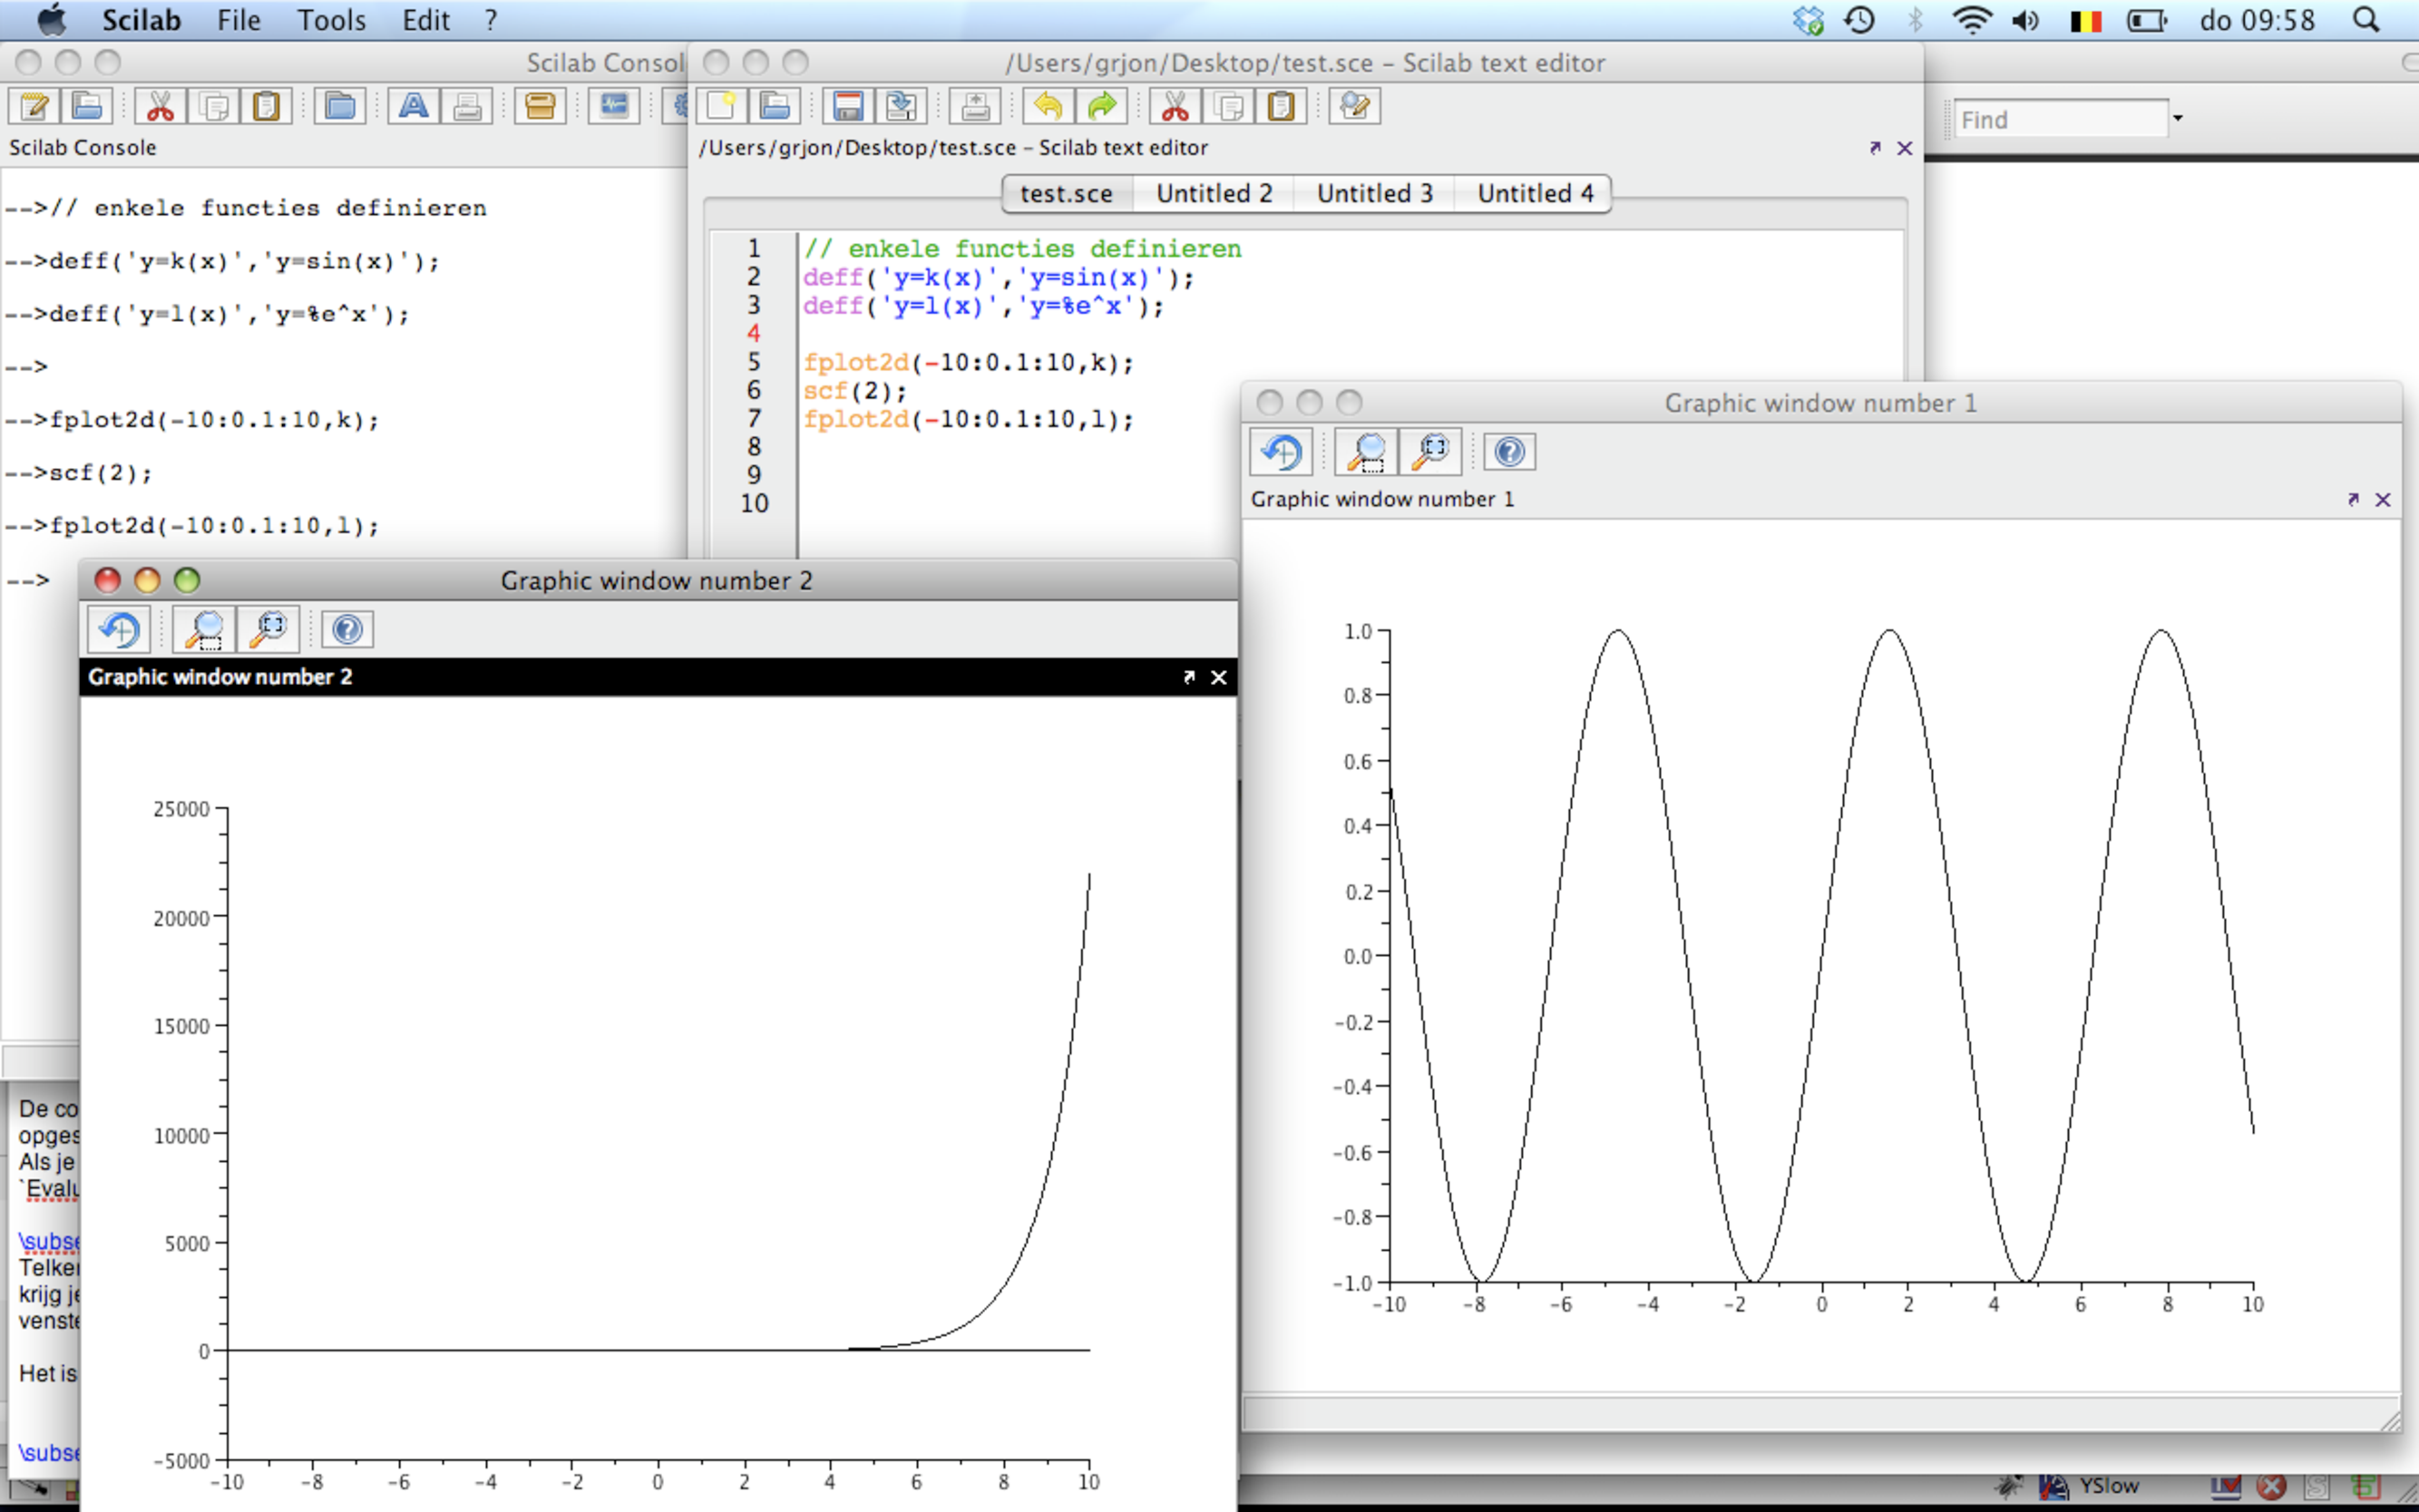
\includegraphics[width=\textwidth]{figuren/scilab/04grafisch_venster}
  \caption{Meerdere grafieken tonen}
	\label{fig:grafisch_venster}
	\end{center}
\end{figure}

\subsection{Het help venster}
Scilab beschikt over een uitgebreide helpfunctie. Als je op het vraagteken klikt of \verb+help+ typt in de console, opent een helpvenster met zoekfunctie (figuur \ref{fig:helpvenster}). Je kan ook specifieke informatie vragen over een functie door bijvoorbeeld in de console \verb+help functienaam+ in te typen. Ten slotte kan je in SciNotes een functie selecteren, rechts klikken en kiezen voor `help on selection' (zie figuur~\ref{fig:helpOnSelection}). Het help-venster opent zich en toont de info over de geselecteerde functie.

\begin{figure}[h!t]
   \begin{center}
    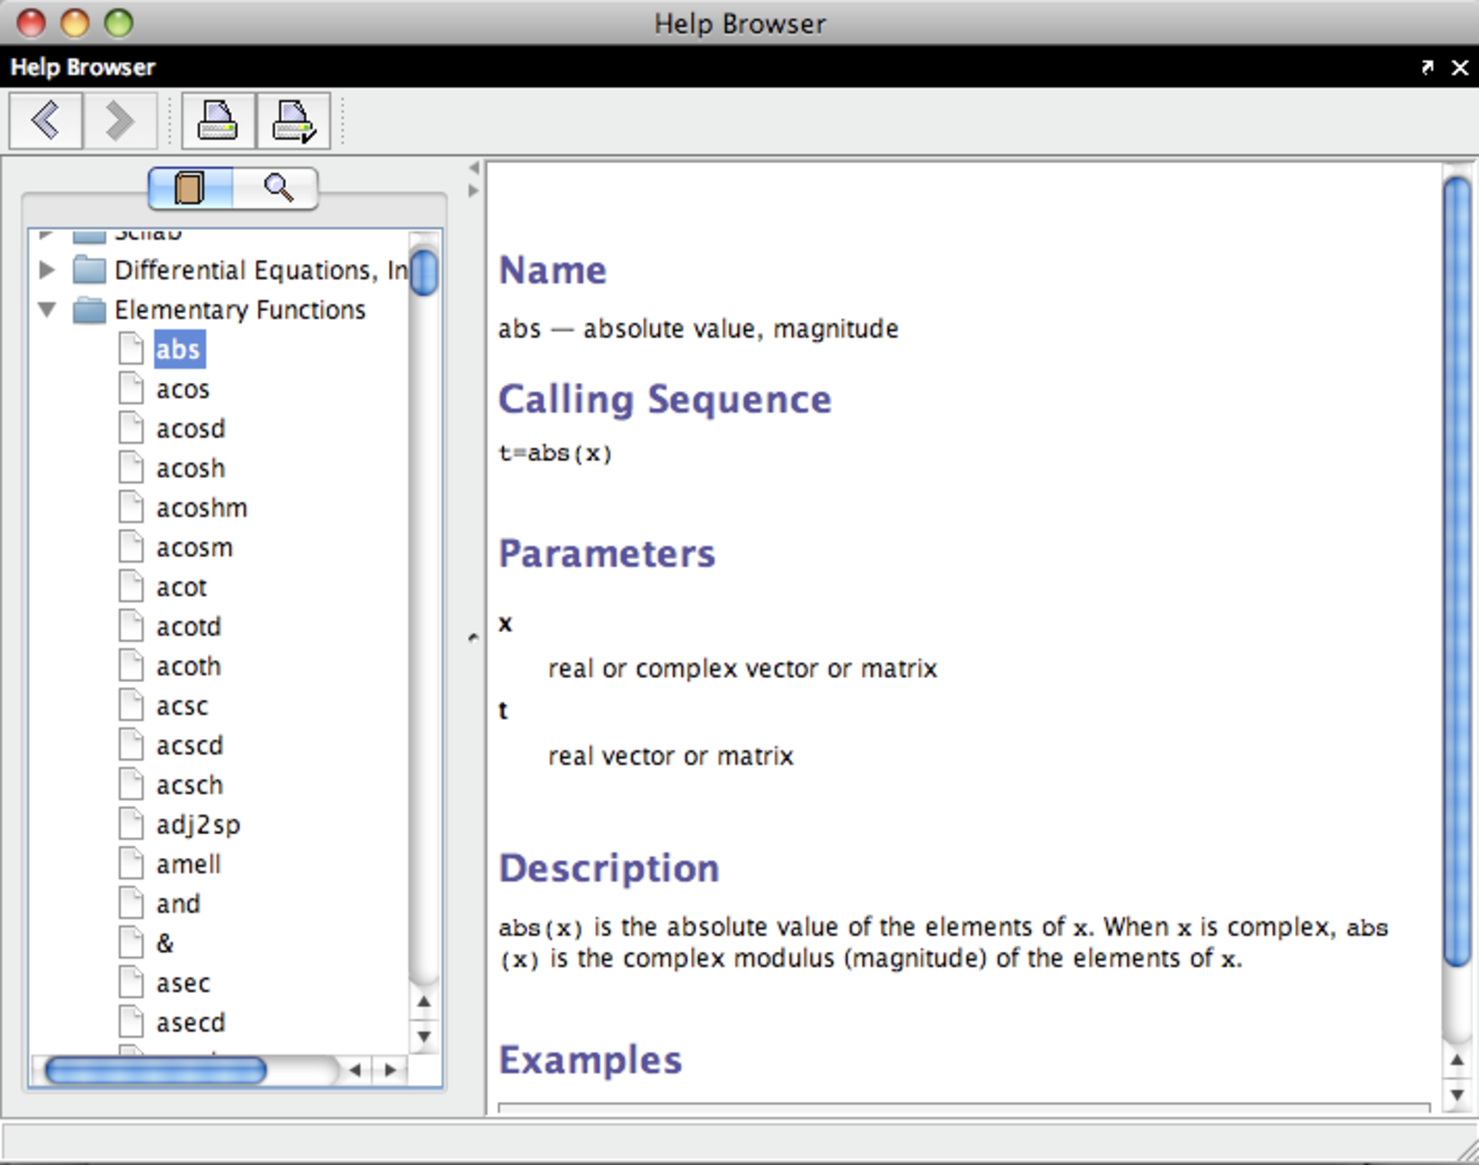
\includegraphics[width=\textwidth]{figuren/scilab/05helpvenster}
  \caption{Het helpvenster}
	\label{fig:helpvenster}
	\end{center}
\end{figure}

\begin{figure}[htbp]
\centering
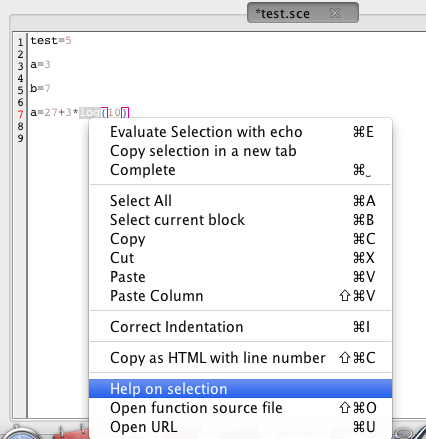
\includegraphics[width=0.7\textwidth]{figuren/scilab/05bhelp_in_scinotes}
\caption{`Help on selection' in SciNotes}
\label{fig:helpOnSelection}
\end{figure}

\subsection{Het scherm met veranderlijken}
Het scherm met veranderlijken (`variable window', figuur~\ref{fig:05cvariableWindow}) toont alle veranderlijken die je tot nog toe gedefinieerd hebt. Als je dubbelklikt op een naam, kan je de waarde aflezen. 
\begin{figure}[htbp]
\centering
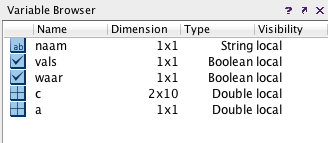
\includegraphics[width=0.7\textwidth]{figuren/scilab/05cvariableWindow}
\caption{Het scherm met veranderlijken}
\label{fig:05cvariableWindow}
\end{figure}

\subsection{Commando overzicht}
Het commando overzicht toont een chronologisch overzicht van de commando's die je tijdens de huidige sessie uitvoerde (`command history'). Als je op een commando dubbelklikt, wordt het opnieuw uitgevoerd. Je kan rechts klikken op een commando en dan kiezen dat je kopieert naar SciNotes.

\subsection{Verschillende vensters combineren}

Doordat je met verschillende vensters tegelijk werkt (console, editor, grafisch venster etc) wordt je scherm al snel een warboel. Je kan de verschillende kleine vensters ook combineren tot één groot venster (figuur~\ref{fig:verschillendevensters}). Neem een venster vast met de muis bij de \emph{blauwe} balk bovenaan en sleep het naar de gewenste positie in een ander venster. Als je het bronvenster laat samenvallen met het doelvenster, worden beide vensters over mekaar geplaatst en kan je van het ene venster naar het andere gaan door middel van de tabs. Als je verschillende vensters van de editor opent, verschijnen ook de tabs (zie figuur~\ref{fig:06bverschillendevensters}). 

\begin{figure}[h!t]
   \begin{center}
    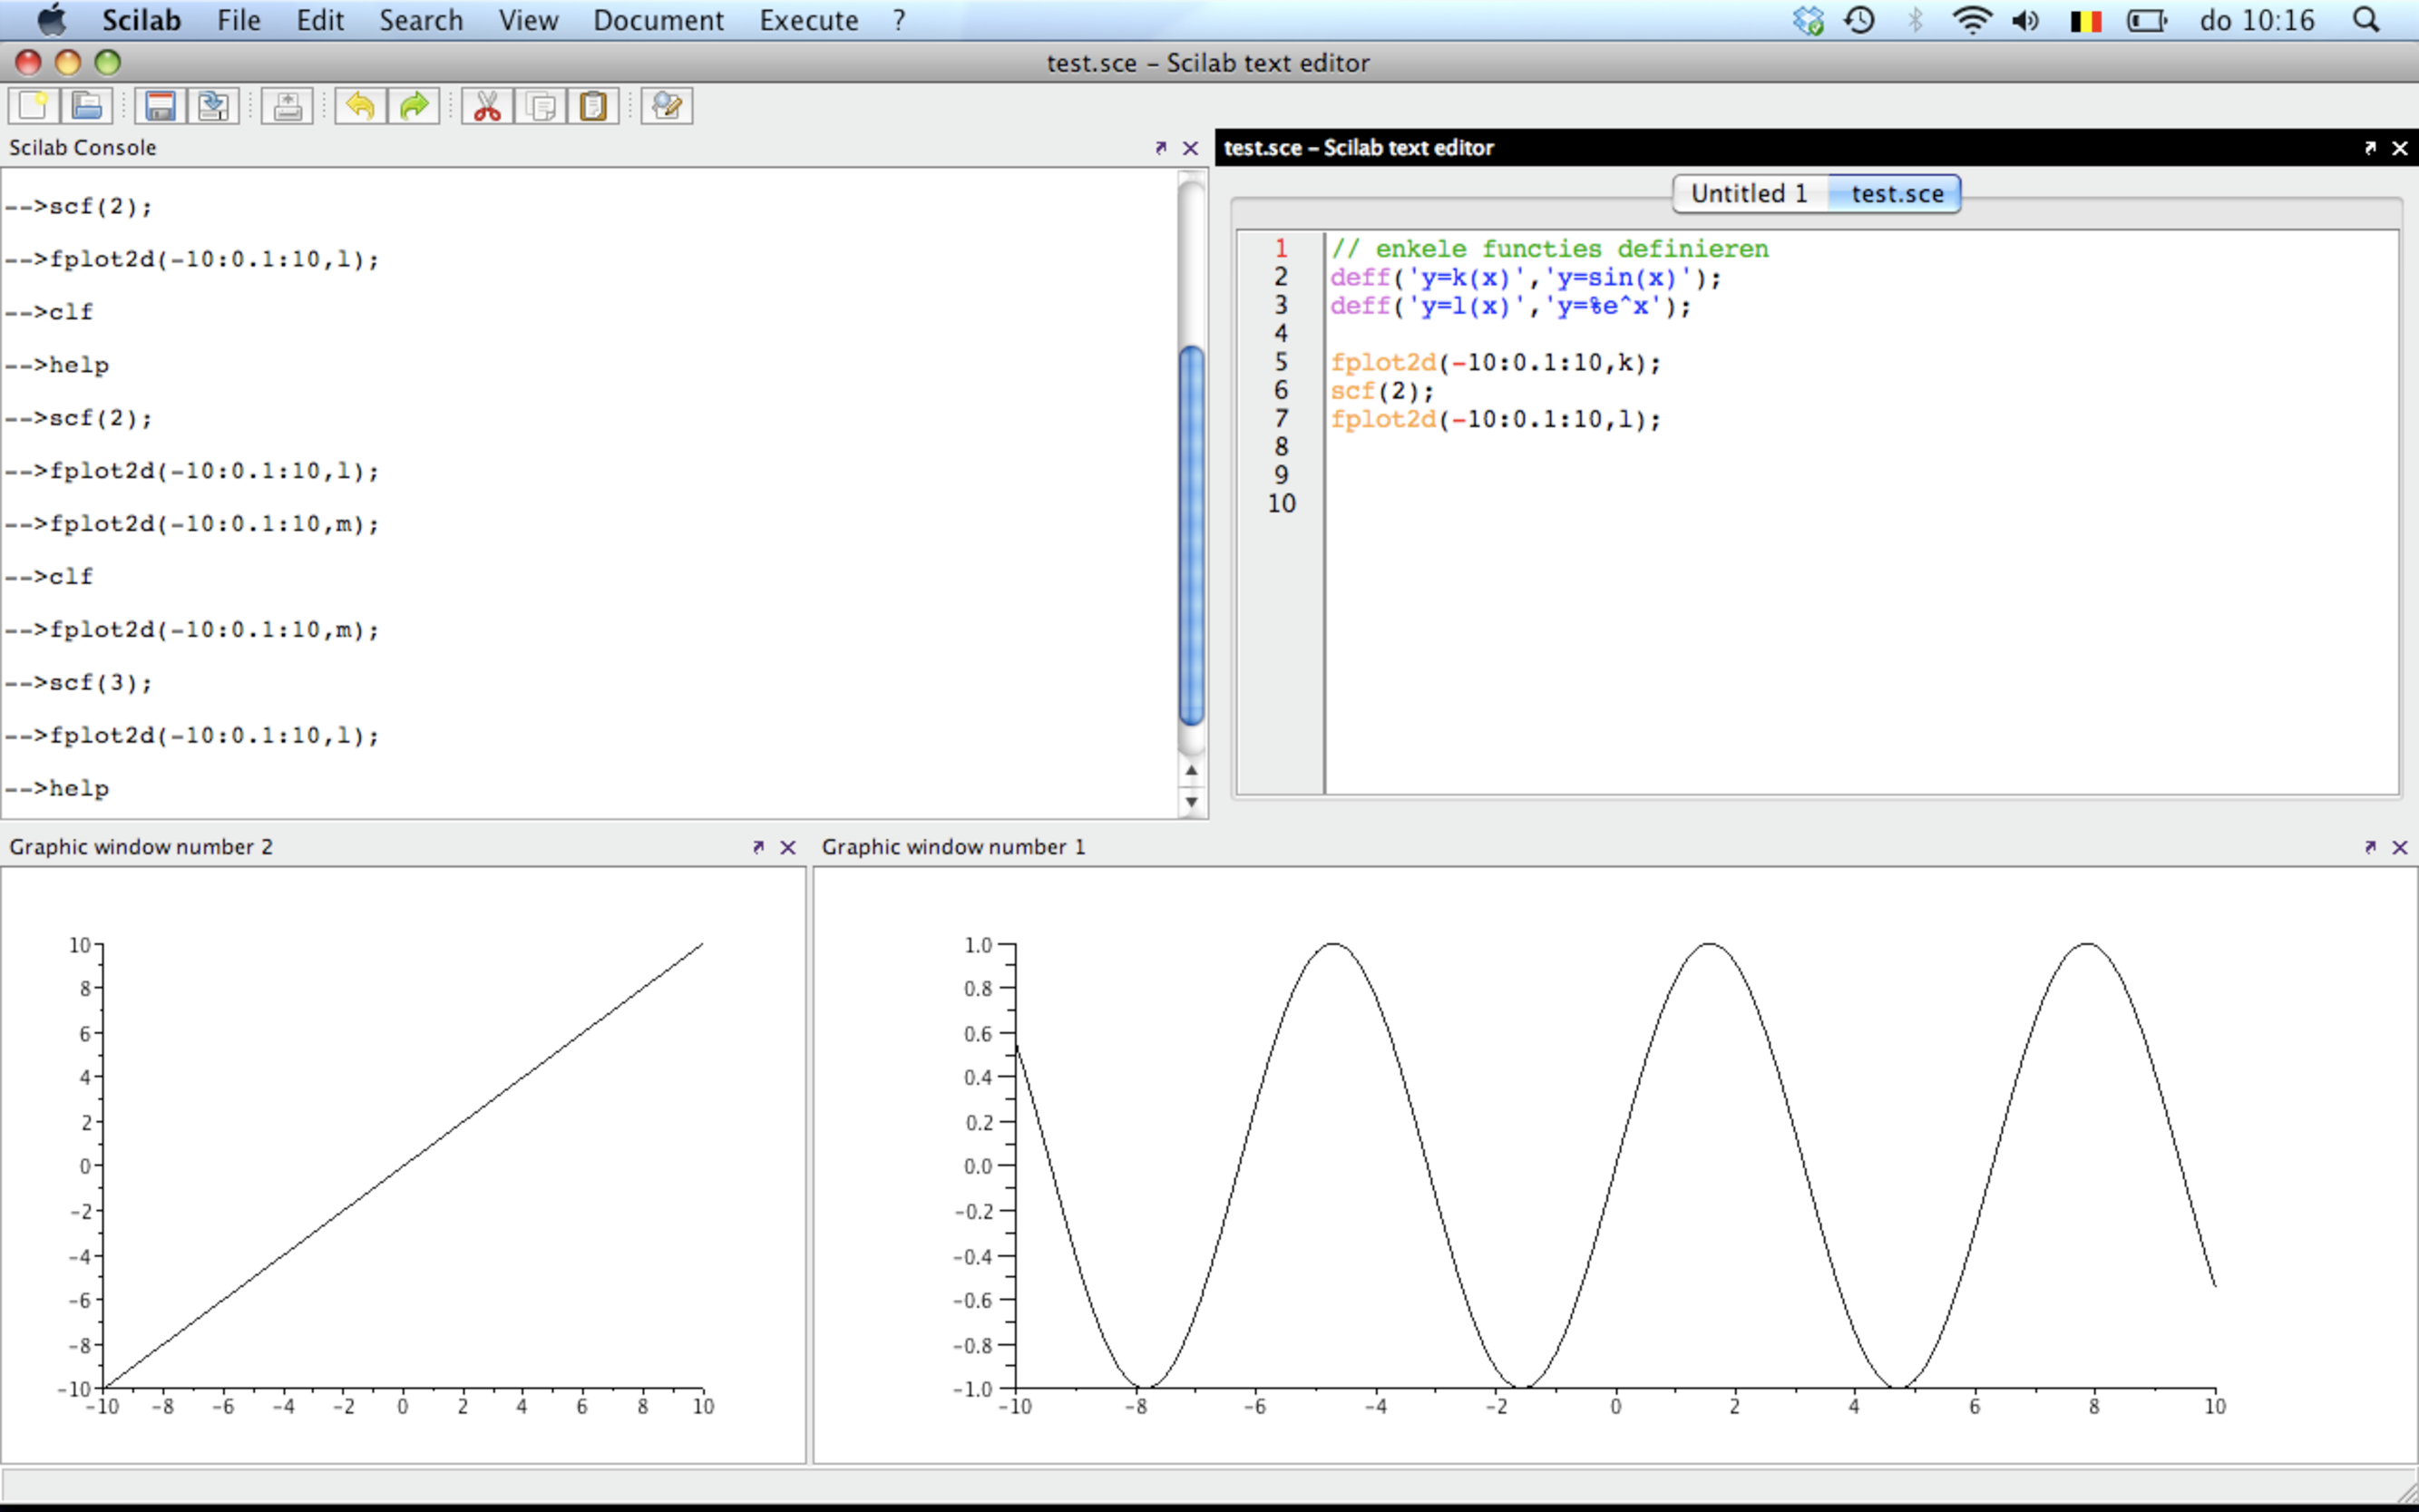
\includegraphics[width=\textwidth]{figuren/scilab/06verschillendevensters.pdf}
  \caption{Verschillende vensters gecombineerd in één venster}
	\label{fig:verschillendevensters}
	\end{center}
\end{figure}

\begin{figure}[htbp]
\centering
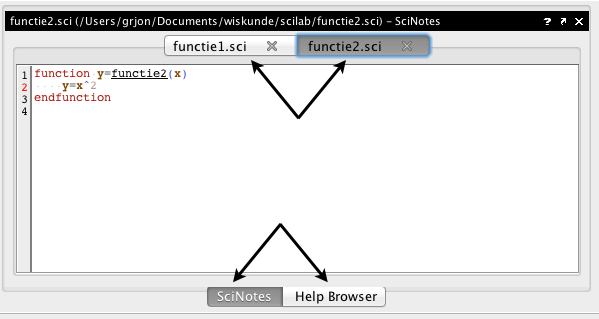
\includegraphics[width=\textwidth]{figuren/scilab/06bverschillendevensters}
\caption{Er verschijnen tabs als je verschillende vensters over mekaar plakt}
\label{fig:06bverschillendevensters}
\end{figure}

%\clearpage
\section{Werken met variabelen}
Variabelen hoeven in Scilab niet eerst gedeclareerd te worden. Een variabele is wel pas gekend als er een waarde aan toegekend is.

\begin{lstlisting}[caption={Foutmelding bij niet-gedefinieerde variabele}, label=Foutmelding bij niet-gedefinieerde variabele]
-->a
  !--error 4 
Undefined variable: a
\end{lstlisting}

Als er een waarde toegekend wordt aan \verb+a+ is er geen foutmelding meer.
\begin{lstlisting}[caption={De waarde van een variabele}, label=De waarde van een variabele]
-->a=%pi/4;
 
-->a
 a  =
 
    0.7853982  
\end{lstlisting}

De naam van een variabele kan bestaan uit meerdere karakters. Een waarde toekennen aan de variabele gebeurt d.m.v.\ `='. Als deze variabele nadien gebruikt wordt in wiskundige uitdrukkingen, dan wordt er gewerkt met de waarde van de variabele. 

\begin{lstlisting}[caption={Waarde van variabelen}, label=waardevanvariabelen]
-->x=-2,3*x^3-1
  x =
     
     -2.
  ans =
     
     -25.
\end{lstlisting}

Als er geen naam toegekend wordt aan een berekening, wordt de waarde automatisch toegekend aan de veranderlijke \verb+ans+.
\begin{lstlisting}[caption={De variabele ans}, label=ans]
-->257/3
 ans  =
 
    85.666667  
 
-->y=ans*3
 y  =
 
    257.  
\end{lstlisting}

Scilab kent verschillende datatypes. De belangrijkste in het kader van dit OPO zijn real, boolean, integer, string en matrices. Er zijn verschillende functies beschikbaar om het datatype van een veranderlijke te testen (bijvoorbeeld isnum, isletter). We merken op dat intern in het systeem alle veranderlijken opgeslagen worden als matrix (zie sectie~\ref{sec:scilabMatrices}). 

Als je het zou willen, zou je aan dezelfde variabele  achtereenvolgens een ander datatype kunnen toekennen. Dit wordt geïllustreerd in listing~\ref{datatype}.

\begin{lstlisting}[caption={Verschillend datatype toekennen aan dezelfde veranderlijke}, label=datatype]
-->x=1
 x  =
    1.  
-->x+1
 ans  =
    2.  
-->x='voor'
 x  =
 voor   
-->x+'deur'
 ans  =
 voordeur  
 \end{lstlisting}



\section{Vectoren en matrices}
\label{sec:scilabMatrices}
Een vector is een geordende verzameling van getallen. In programmeervakken noem je dit meestal een \emph{eendimensionale array}. Een voorbeeld:
\begin{displaymath}
V=[1,2,3,4,5]
\end{displaymath}
Een matrix is een rechthoekig schema getallen (\emph{tweedimensionale array}). 
\begin{displaymath}
M=\begin{bmatrix}
 1&2  &-3 &2 \\
 8& 5 &7 &5 \\
 -6& -4 &11&8
\end{bmatrix}\,.
\end{displaymath}

Bovenstaande matrix bijvoorbeeld bevat 3 rijen en 4 kolommen. In Scilab wordt een matrix  rij per rij genoteerd tussen vierkante haken `\verb+[,]+'. De kolommen worden gescheiden door `\verb+,+' en de rijen door `\verb+;+'. Het aantal rijen en kolommen wordt opgevraagd door de functie \verb+size()+. Merk op dat deze functie als antwoord een vector met twee elementen geeft.

\begin{lstlisting}[caption={Een matrix defini\"eren}, label=Matrixdef]
-->M=[1,2,-3,2;8,5,7,5;-6,-4,11,8]
 M  =
 
    1.    2.  - 3.     2.  
    8.    5.    7.     5.  
  - 6.  - 4.    11.    8.  
  
  -->size(M)
 ans  =
 
    3.    4.  
\end{lstlisting}

Als de vector bestaat uit een \emph{rij opeenvolgende getallen of een rekenkundige rij}, volstaat het om de korte notatie met `\verb+:+' te gebruiken (zie listing~\ref{korte_notatie}). Als het verschil gelijk is aan 1, hoeft het niet expliciet vermeld te worden (eerste voorbeeld). Als het verschil een ander getal is, moet het expliciet vermeld worden (tweede voorbeeld). Vierkante haken mogen, maar zijn niet nodig.
\begin{lstlisting}[caption={Een matrix defini\"eren: korte notatie}, label=korte_notatie]
-->B=[1:8]
 B  =
 
    1.    2.    3.    4.    5.    6.    7.    8.  
 
-->C=3:-0.5:0
 C  =
 
    3.    2.5    2.    1.5    1.    0.5    0.  
 
\end{lstlisting}


Een matrixelement wordt opgevraagd door de indices te geven, bvb.: \verb+M(1,2)+ (let op: hier ronde haakjes gebruiken). Dit is het element in de eerste rij, tweede kolom. In bovenstaand geval zou dit \verb+2+ opleveren. In tegenstelling tot programmeertalen als Java en PHP heeft het eerste element uit een rij index 1 en niet index 0. 
Een vector is niets meer dan een matrix bestaande uit 1 rij of 1 kolom. Om een element uit een vector te halen moet je slechts \'e\'en index meegeven.

Scilab kent heel wat ingebouwde functies voor matrices en vectoren. In tabel~\ref{tabel:matrices} sommen we er enkele op.

\begin{table}[h] \small
\centering
\caption{Enkele ingebouwde functies m.b.t.\ matrices}
\begin{tabular}{p{7.cm}p{4.cm}}
\toprule

definitie matrix    &   \verb+M=[1,2,3,4;5,6,7,8]+ \\

matrixelement       &   \verb+M(2,3)+\\

volledige rij van een matrix    & \verb+M(3,:)+\\

submatrix           & \verb+M(1:2,2:3)+\\

matrices samenvoegen: onder mekaar            & \verb+M=[A;B]+\\
matrices samenvoegen: langs mekaar            &\verb+M=[A,B]+\\
matrix transponeren (rijen$\leftrightarrow$kolommen) & M'\\

constante optellen bij elk element & \verb/M+3/ \\

elk element vermenigvuldigen met constante & \verb+M*3+ \\

matrixoptelling: element per element	& \verb/M+N/\\

matrixvermenigvuldiging 	& \verb/M*N/\\
$\qquad$(let op de dimensies!)&\\

matrixvermenigvuldiging: 	& \verb/M.*N/\\
$\qquad$element per element&\\

macht van een matrix	& \verb/M^2/\\
$\qquad$element per element&\\

matrix met $4$ rijen en $2$ kolommen,               & \verb+zeros(4,2)+ \\
$\qquad$ieder element gelijk aan $0$ &\\

idem, maar ieder element gelijk aan $1$ & \verb+ones(4,2)+ \\

idem, ieder element random tussen 0 en 1 & \verb+rand(4,2)+ \\
lengte van de vector $V$ & \texttt{length(V)} \\
aantal rijen en kolommen van de matrix $A$ & \texttt{size(A)} \\
elementen van $A$ sorteren&\texttt{gsort(A)}\\
elementen van $A$ kleiner dan 5, gelijk aan 3& \verb+find(A<5)+, \verb+find(A==3)+\\
\bottomrule
\end{tabular}
\label{tabel:matrices}
\end{table}

Zoek in de help van Scilab welke opties de functies \verb/gsort/ en \verb/find/ bieden. 


\section{Functies}

\subsection{Definitie van een functie}
\label{sec:werken_met_functies}
De definitie van een functie begint met \verb+function+ en eindigt met \verb+endfunction+. In listing~\ref{Functiedef} definiëren we de functie \verb+dollars+ die het bedrag \verb+e+ in euros omzet naar het bedrag \verb+d+ in dollars. De variabele \verb/t/ is de koerswissel, \verb/e/ en \verb+t+ zijn de \emph{variabelen}; \verb/d/ is het \emph{resultaat} (de return-waarde).
\begin{lstlisting}[caption={Functie defini\"eren}, label=Functiedef]
-->function d=dollars(e,t);
-->  d=e*t;
-->endfunction
 
-->dollars(200,1.2)
 ans  =
 
    240.  
\end{lstlisting}

Listing~\ref{Functiedef} toont een functiedefinitie in het consolevenster. \emph{Dat is niet de beste manier van werken}, maar het kan wel
voor functies die maar uit een paar regels tekst bestaan.

Voor een eenvoudige functie kan je ook  het commando \verb+deff+ gebruiken om een functie te defini\"eren in de commandolijn:
\begin{lstlisting}[caption={Functie defini\"eren met deff}, label=functiedeff]
-->deff('y=g(x)','y=x^2-1')

-->g(3)
 ans  =
 
    8.   
\end{lstlisting}

In de eerste string geef je mee dat je de functie \verb+g+ definieert die \verb+x+ als parameter heeft. In de tweede string (\verb+'y=x^2-1'+) zeg je hoe deze functie gedefinieerd is.

\subsection{Interactie met de gebruiker}

Soms verwacht een functie input van de gebruiker. Hiervoor kan je de functie \verb+input()+ gebruiken. Met dit commando wacht het programma op een waarde die via het toetsenbord wordt ingegeven. 

Met de functie \verb+disp+ kan je verzorgde output leveren. De functie \verb+string()+ verandert het datatype naar een string. Met het \verb/+/-teken plak je verschillende strings aan mekaar. Je kan ook de functie \verb/printf()/ gebruiken. Dit wordt geïllustreerd in figuur~\ref{fig:input}. Om output naar een bestand te schrijven gebruik je de functie \verb+fprintf()+. Zie de helpfunctie voor meer informatie.

\begin{figure}[h!t]
   \begin{center}
    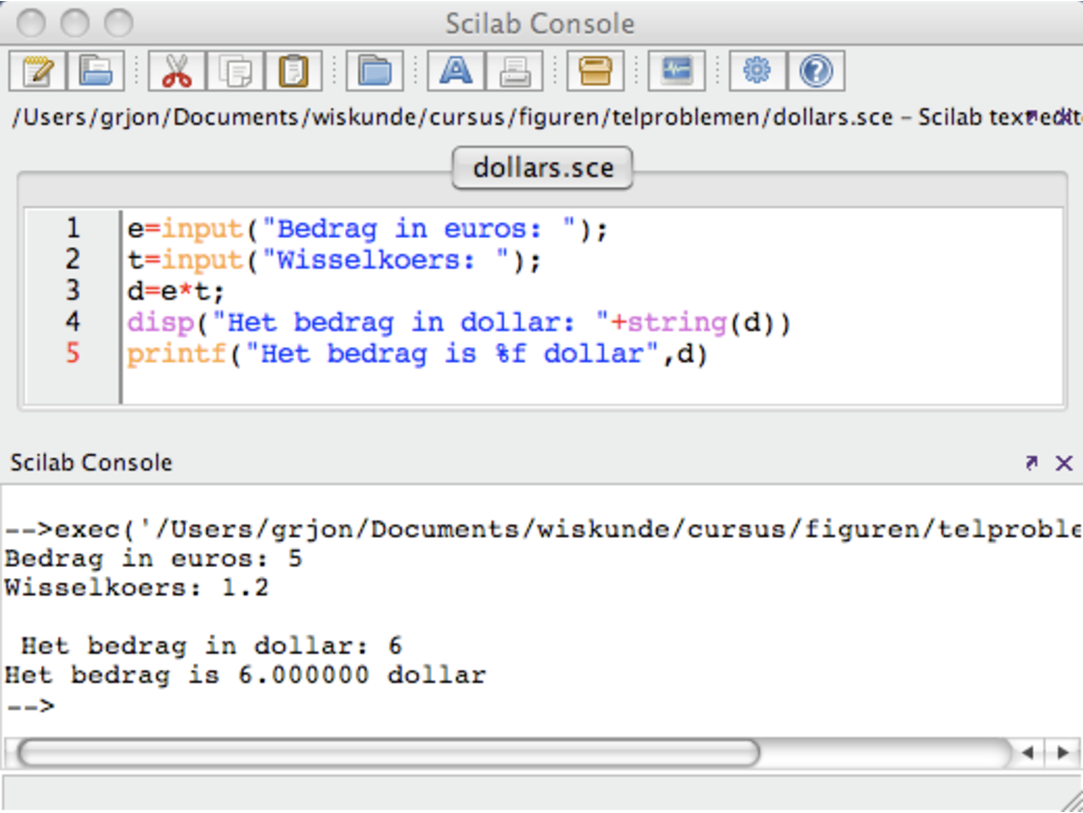
\includegraphics[width=\textwidth]{figuren/scilab/07input.pdf}
  \caption{Interactie met de gebruiker}
	\label{fig:input}
	\end{center}
\end{figure}

\subsection{Grafieken}
\label{sec:grafiek}
De grafiek van een functie is --\,naast de tabel en het functievoorschrift\,-- een handig middel om het verloop (nulpunten, stijgend en dalend, \dots) van de functie te beschrijven. De grafiek geeft een globaal beeld van de functie op een bepaald interval.

De ingebouwde functie \verb+plot(vec,function)+ genereert eenvoudig grafieken van functies.
De veranderlijke \verb+vec+ is een vector. Voor alle elementen van deze vector wordt de
functiewaarde berekend en in het grafisch venster geplot (zie figuur~\ref{figg:functie1}):

\begin{center}
\begin{minipage}{.95\linewidth}
\begin{lstlisting}[caption={Functiedefinitie en plot}, label={Functiedefinitieenplot1}]	
function y=f(x)
  y=(x^2+2*x)*exp(-x)
endfunction
x=-2:0.2:5;
plot(x,f)
\end{lstlisting}
\end{minipage}
\end{center}

\begin{figure}[h!t]
   \begin{center}
  \includegraphics[width=0.8\textwidth]{figuren/scilab/08grafiek.pdf}
  \caption{Grafieken tekenen: resultaat van listing~\ref{Functiedefinitieenplot1}}
	\label{figg:functie1}
	\end{center}
\end{figure}


Merk op dat, als je twee maal achter mekaar \verb+plot+ invoert, beide grafieken over mekaar getekend worden.
Het commando \verb+clf+ (clear figure) zorgt ervoor dat het grafisch venster `opgeschoond' wordt. 

Ten slotte kan je je grafiek opfleuren met een titel, gridlijnen en kleurtjes (zie figuur~\ref{figg:meerderf}). In Windows kan je eenvoudig de eigenschappen van de grafieken wijzigen met het menu-item edit - figure properties (zie figuur~\ref{fig:11bgrafiek}). 
\begin{figure}[htbp]
\centering
\includegraphics[width=\textwidth]{figuren/scilab/11bgrafiek}
\caption{De eigenschap van een grafiek veranderen met het venster voor eigenschappen}
\label{fig:11bgrafiek}
\end{figure}

Als je de eigenschappen van de grafiek niet via het menu kan wijzigen, kan je dat doen met behulp van de functie \verb+gda()+. Deze functie creëert een object met alle eigenschappen van de grafiek zoals kleuren, achtergrondvulling, al dan niet een titel etc. Voer het commando uit in de prompt om zijn waarde te kennen (zonder puntkomma!) en test zelf een aantal mogelijkheden uit.


\begin{lstlisting}[caption={Meerdere functies in \'e\'en grafiek}, label=meerderefunctiesplotten]	
function y=f(x)
  y=(x^2+2*x)*exp(-x)
endfunction
function y=g(x)
  y=sin(x/2)
endfunction
x=-2:0.1:5;
clf;
a=gda(); 
a.x_location="middle";
a.y_location="middle";
xtitle("De functies f(x) en g(x)");
xgrid(0); //het cijfer geeft de kleur aan
plot(x,f);
plot(x,g,'r');
\end{lstlisting}

\begin{figure}[h!t]
   \begin{center}
    \includegraphics[width=0.8\textwidth]{figuren/scilab/10grafiek.pdf}
  \caption{Grafieken tekenen: resultaat van listing~\ref{meerderefunctiesplotten}}
	\label{figg:meerderf}
	\end{center}
\end{figure}


 
Nog een voorbeeld vind je in figuur \ref{figg:vierkant} (vooral te gebruiken in 2Ti). We maken hier gebruik van de functie \verb+plot2d+ om meer opties te bekomen.
\begin{lstlisting}[caption={Vierkant tekenen}, label=plot2d]	
clf;
a=gda(); 
a.x_location="bottom";
a.y_location="left";
// er moet rekening gehouden worden met de data_bounds
a.tight_limits="on";
// definieer de x- en y-range van de assen
a.data_bounds=[0,5,0,5];
// Definieer een titel en zorg ervoor dat hij getoond wordt
a.title.text="Een rechthoek";
// toon gridlijnen
xgrid(0);
a.thickness=1;
a.font_size=0.5;
x=[2,2,4,4,2]; y=[0,2,2,0,0];
plot2d(x,y)    
 \end{lstlisting}
 
\begin{figure}[h!t]
   \begin{center}
    \includegraphics[width=0.8\textwidth]{figuren/scilab/11grafiek}
    \caption{Vierkant tekenen met plot2d}
	\label{figg:vierkant}
	\end{center}
\end{figure}

Scilab voorziet eindeloos veel mogelijkheden om figuren aan te passen en leesbaarder te maken met kleurtjes en titels. Typ bijvoorbeeld \verb+help plot2d+ of \verb+help gda+ in de prompt en bekijk de voorbeelden die de helpfunctie geeft.
 
 We vermelden ten slotte de functie \verb/xclick()/. Als je dit commando in de prompt ingeeft, kan je op een plaats in de grafiek klikken. Het resultaat bestaat uit drie getallen. Het eerste geeft aan met welke muisknop je geklikt hebt. De twee andere getallen geven de coördinaten aan van het punt waarop je geklikt hebt.

\section{Programmeren in Scilab}
\subsection{Functies}

We spreken over \emph{programma's}, maar eigenlijk is dat geen correcte term. In Scilab maak je nieuwe \emph{functies}. Het equivalent in Java is een \emph{methode}. 

Een functie heeft een \emph{functienaam}, een \emph{(aantal) argument(en)}, ook wel gekend als \emph{parameter(s)} en een \emph{functiedefinitie}. Elke functie heeft juist \'e\'en resultaat (zoals we later gaan zien kan dit resultaat wel bestaan uit meerdere getallen). In 
sectie~\ref{sec:werken_met_functies} vermeldden we reeds hoe je functies definieert en oproept in Scilab.


Het is belangrijk dat je de functies voldoende documenteert. Documentatie voer je in na \verb+//+. Tekst rechts hiervan wordt niet gelezen. 

\begin{lstlisting}[caption={Elke functie bevat enkele regels uitleg!}, label=Maal.sci]
function y=maal(a,b)
// deze functie berekent a*b
//
//Input Arguments:
//  a           een integer; de eerste factor
//  b           een integer; de tweede factor

y=a*b
endfunction
\end{lstlisting}

Als je een boodschap wil meegeven aan de gebruiker  kan dit met het \verb+disp+ commando. Het gebruik: \verb+disp("foutmelding")+. In listing~\ref{fac} vind je een voorbeeld. Met het commando \verb+abort+ beëindig je het programma. Je kan beide commando's samen ook vervangen door de functie \verb/error("message")/. Het programma toont de foutboodschap en keert terug naar de prompt. 


\subsection{Lussen: while en for}
De twee voornaamste lussoorten zijn 
\verb+while+ en \verb+for+. Met het sleutelwoord \verb+break+ ga je uit de lus, bijvoorbeeld wanneer je na een controle met een \verb+if+ het resultaat bekomen hebt dat je wou. Probeer het gebruik van \verb/break/ wel te vermijden, want dat geeft al snel aanleiding tot `spaghetticode'. Meestal kan het vervangen worden door een doordacht gebruik van een \verb/while/-lus.

\begin{lstlisting}[caption={Eenvoudig voorbeeld van een whilelus}, label=simpele while]
function y=testwhile(x)
  // toon de waarden van 1 t.e.m. x op het scherm
  // x moet groter of gelijk aan 1 zijn
  y=1;
  disp(y) 		// toon de waarde van y op het scherm
  while y<x
    y=y+1;
    disp(y)
  end
endfunction
\end{lstlisting}

Vorig voorbeeld is nogal eenvoudig maar het toont wel hoe een whilelus in elkaar zit. Je moet eerst de variabele $y$ initialiseren; je geeft de conditie aan van de lus. Binnen de lus geef je aan wat er moet gebeuren, en belangrijk, $y$ moet opgehoogd worden. Anders zit je met een \emph{oneindige lus}.

Een volgend voorbeeld gaat over de \verb+for+-lus.

\begin{lstlisting}[caption={Eenvoudig voorbeeld van een for-lus}, label=simpele for]
function y=testfor(x)
  // zelfde als hierboven, maar met for-lus
  
  for y=1:x
    disp(y)
  end
endfunction
\end{lstlisting}

Zoals je kan zien is een \verb+for+-lus gelijkaardig aan de \verb+while+-lus. Er zijn echter een aantal verschillen. Zo kan de variabele $y$ ge\"initialiseerd worden binnen de \verb+for+ zelf met \verb+y=1+. De conditie is ook anders dan in de while. In de for gebruik je `:' wat zo veel wil zeggen als `tot'. Je zegt dus eigenlijk dat $y$ gaat van 1 tot x. In de lus zelf mag $y$ niet opgehoogd worden: dit gebeurt door de \verb+for+-lus zelf.

\subsection{Controlestructuren}
Scilab kent het \verb+if+-statement. Een \verb+if+-statement wordt afgesloten d.m.v.\ een \verb+end+. If-statements kunnen ook genest worden. Het woordje \verb+then+ is optioneel. Als je het schrijft, moet het op dezelfde regel als de \verb+if+ staan.

\begin{lstlisting}[caption={Geneste if}, label=geneste if]
function y=verwerk(x)

if modulo(x,2) == 0
  if x==2
    y = 1
  elseif x == 4
    y = 2
  else
    y = 0
   
  end
  
elseif modulo(x,3) == 0
  y = 0
else
  y = -1
end

endfunction
\end{lstlisting}

Je merkt dat \verb+if+ afgesloten wordt met \verb+end+. Tussen
begin en einde kan je de nodige bewerkingen uitvoeren.

Er bestaan twee mogelijkheden om een alternatief te laten
uitvoeren. Als er maar \'e\'en alternatief is, gebruik je
\verb+else+. Indien er verschillende alternatieven zijn (bvb.\  $x>0$ en $x=0$), kan je \verb+elseif+ gebruiken.
Achter \verb+elseif+ typ je de te controleren voorwaarde en
vervolgens de bewerkingen indien aan de voorwaarde voldaan is.
Merk op dat \verb+elseif+ \emph{niet} afgesloten wordt met
\verb+end+.

In tabel~\ref{operatoren-scilab} vind je de belangrijkste logische
operatoren. De {\sc en}- en {\sc of}-operator heeft voorrang op de andere operatoren. Vergeet dus geen haakjes te plaatsen, bvb.\ \verb/(x>3)&(x<5)/. Let ook op het verschil tussen de \emph{toekenningsoperator} \verb+a=b+ en de \emph{logische operator} \verb+a==b+.

\begin{table}[htbp]
\centering
\caption{Logische operatoren in Scilab}
\begin{tabular}{ll}
\toprule

             & Scilab \\ 
\midrule
{\sc en, of, niet} &\verb/ &, |, ~/ \\ 
$\neq,~=$ & \verb/<>, ==/ \\ 
$<,~>,~\leq,~\geq$    & \verb/<, >, <=, >=/ \\ 
{\sc true, false}&\verb+%T, %F+\\ 
\bottomrule
\end{tabular}
 \label{operatoren-scilab}
\end{table}




\subsection{Programmeren met vectoren}

Binnen een lus kan je bewerkingen doen op ieder vectorelement. Eerst moet de vector gedefinieerd zijn. Dit kan met de functie \verb+zeros(1,n)+ waarbij \verb+n+ op voorhand moet ingevuld zijn. Onderstaand programma berekent de faculteit van de getallen 1 t.e.m. \verb+n+. Het resultaat is een vector $V_{i} = i!$.

\begin{lstlisting}[caption={Bereken faculteit van 1 t.e.m. x}, label=fac]
function V=facvector(x)
// bereken faculteit van 1 t.e.m. x
 
 if x<0; 
   disp("faculteit van negatief getal bestaat niet: 
   	de input is "+string(x))
    abort 
 // foutmelding
  else
    V=zeros(1,x); // vector definieren
    V(1)=1;       // fac(1)=1
    for i= 2 : x
      V(i)=V(i-1)*i;
    end
  end;
endfunction
\end{lstlisting}

Volgend programma berekent het grootste element van een vector:

\begin{lstlisting}[caption={Maximum van een vector}, label=maximum]
function y=maximum(V)
// berekent het grootste getal van de vector V
y=V(1);
for i=2 : length(V)
  if V(i)>y
    y=V(i)
  end
end
endfunction
\end{lstlisting}

In listing~\ref{fac} initialiseren we de vector $V$ met de functie \verb/zeros()/. Dat is enkel mogelijk als het aantal elementen van de resulterende vector gekend is. Als dat niet zo is, moet de vector $V$ geïnitialiseerd worden als een lege vector. Nadien worden de elementen één na één toegevoegd. Als voorbeeld schrijven we de functie \verb/cijfers(V)/. Input is de vector \verb+V+ van willekeurige lengte die de cijfers 0 tot en met 9 bevat. Output is een vector die alle cijfers die voorkomen in \verb/V/ juist één keer bevat van klein naar groot.
Dit wordt getoond in voorbeeld listing~\ref{lege_vector}.

\begin{lstlisting}[caption={Een vector aanmaken gedurende de functie}, label=lege_vector]
function W=cijfers(V)
  // output initialiseren
  W=[];
  // controleren of V enkel cijfers 0:9 bevat
  for i=1:length(V)
    if (V(i)<0)|(V(i)>9)
      disp('input mag enkel cijfers tussen 0 en 9 bevatten')
      abort // foute input, dus functie afbreken
    end
  end
  // cijfer per cijfer controleren of het voorkomt in V
  for i=0:9
    for j=1:length(V)
      if V(j)==i
        W=[W,i] // cijfer komt voor, dus plakken aan output-vector
        break // cijfer is gevonden, dus niet meer verder zoeken
        // voor dit cijfer
      end
    end
  end
endfunction
\end{lstlisting}

\subsection{Meerdere waarden als resultaat van een functie}
Een functie heeft steeds \'e\'en resultaat maar dit resultaat mag ook \emph samengesteld zijn uit verschillende getallen, zoals een vector. Een volgend voorbeeld zoekt zowel naar het kleinste als het grootste getal in een vector.

\begin{lstlisting}[caption={Minimum en maximum van een vector}, label=minenmax]
function [minim,maxim]=extrema(V)
// berekent het kleinste en het grootste getal 
// van de vector V
maxim=V(1);
minim=V(1);
for i=2 : length(V)
  if V(i)>maxim
    maxim=V(i);
  end;
  if V(i)<minim
    minim=V(i);
  end
end
endfunction
\end{lstlisting}

We laden de functie in in Scilab en bekijken het resultaat:

\begin{lstlisting}[caption={Het minimum en maximum in het console venster}, label=minenmaxinscilex]
-->V=[1,2,3,5,3,9,6];

-->[mi,ma] = extrema(V)
  ma =
     
     9.
  mi =

     1.
\end{lstlisting}

Aangezien de functie als resultaat een lijst met twee waarden geeft moet je de functieoproep gelijkstellen aan een lijst met twee variabelen (hier mi en ma). Er is echter nog een andere mogelijkheid om een resultaat van meerdere getallen te bekomen: een \emph{vector} of een \emph{matrix}. Dit wordt gedemonstreerd in een volgend voorbeeld.

\begin{lstlisting}[caption={Functie euro(x)}, label=euro]
function G=euro(x)
// berekent het aantal briefjes en stukken om een
// bedrag x in euro te vormen met zo weinig mogelijk
// briefjes of stukken
E=[500,200,100,50,20,10,5,2,1,0.50,0.20,0.10,0.05,0.02,0.01];
G=zeros(size(E));
for i=1 : length(E)
  G(i)=floor(x/E(i));
  x=x-G(i)*E(i);
  if G(i) ~= 0
    disp([E(i),G(i)]) // Uitvoer naar het scherm
  end
end
endfunction
\end{lstlisting}

Deze functie geeft soms echter fouten. Waarom denk je?

\section{Oefeningen}
\begin{oef}
Bereken volgende uitdrukkingen in SciLab: 
\begin{enumerate}
  \item  $\dfrac{4\cdot \pi-7}4 \cdot 2+10$
  \item $\dfrac{ -7^3}8 $
  \item $| - 4| $
  \item mod(7, 3), mod($ -15$, 4) 
  \item floor($-2.45$) 
  \item $500\cdot 1.05^\frac{12}2\cdot \dfrac{1-1.05^\frac{-13}2}{1-1.05^\frac{-1}2} $
\end{enumerate}
\begin{opl}
\begin{enumerate}
  \item 12.783185	
  \item -42.875
  \item 4
  \item 1, -3 
  \item -3
  \item 7555.9475
\end{enumerate}
\end{opl}
\end{oef}

\begin{oef}
Definieer de functie $opp(z)$ die de totale oppervlakte berekent 
van een kubus met zijde $z$. Bereken nu de oppervlakte 
als $z$ gelijk is aan \num{2.5} of \num{3.125}.
\begin{opl}
\code{oefeningen/oppervlakte.sci}
\end{opl}
\end{oef}



\begin{oef}
Een rol behangpapier is \SI{10}{\meter} lang. Stel de veranderlijke~$t$
gelijk aan de hoeveelheid behangpapier die je nodig hebt, uitgedrukt in meter.
Stel \verb/aantalrollen/ het aantal rollen dat je moet kopen om aan de
hoeveelheid $t$ te voldoen. Teken de grafiek van de functie \verb/aantalrollen/.
\begin{opl}
\code{oefeningen/aantalrollen.sci}
\end{opl}
\end{oef}


\begin{oef}
De studentenkring organiseert een voetbalwedstrijd. De materiaalmeester heeft \SI{100}{\meter} lint bij om het voetbalterrein af te spannen. 
\begin{enumerate}
\item Teken de grafiek van de functie \verb/breedte/ die de breedte $b$ van het terrein in functie van de lengte $l$ weergeeft.
\item Teken de grafiek van de functie \verb/opp/ die de oppervlakte $o$ van het terrein in functie van de lengte $l$ weergeeft. Voor welke lengte is de oppervlakte maximaal?
\end{enumerate}
\begin{opl}
\code{oefeningen/voetbal.sci}
Maximumoppervlakte bij \verb'l' = 25.
\end{opl}
\end{oef}


\begin{oef}
(Moeilijker) Er is een misdaad gebeurd. De politie moet twee oppervlakten afspannen. Ze gebruikt daarvoor \SI{60}{\meter} lint. De eerste oppervlakte is cirkelvormig. De tweede oppervlakte is een vierkante oppervlakte die langs \'e\'en zijde aan een muur grenst. Langs de muur hoeft geen lint gespannen te worden. 
\begin{enumerate}
\item Definieer de functie \verb/oppervlakte/ die de afgespannen oppervlakte $opp$ toont in functie van zijde $z$ van het vierkant.
\item Teken deze functie.
\item Wat zijn de afmetingen van cirkel en vierkant opdat de afgespannen oppervlakte minimaal is?
\end{enumerate}
\begin{opl}
\code{oefeningen/misdaad.sci}
Bij minimale oppervlakte: $z = 8.35$ en $r = 5.56$.
\end{opl}
\end{oef}


\begin{oef}
Teken de functies $y = 5^x$ en $y = \frac15^x$ op hetzelfde scherm. 
Zorg voor aangepast bereik van de co\"ordinaatassen. Verzorg ook de titel van de grafiek.
\end{oef} 


\begin{oef}
Herschrijf de functie van \cref{fac} waarbij je te werk gaat zoals in \cref{lege_vector}.
\end{oef}


\begin{oef}
Schrijf de functie  \verb/sommeetk(a,r,n)/, die de som berekent van opeenvolgende elementen van een meetkundige rij.
De veranderlijke $a$ is de eerste term van de som, $v$ is de reden van de meetkundige rij en de som 
bevat $n$ termen. Geef als output  de som en de laatste term van de som.
(meervoudige output). Gebruik eerst de \verb/for/-lus , daarna  de \verb/while/-lus.
\begin{opl}
\begin{samepage}
Met een {\tt for}-lus:
\code{oefeningen/sommeetk-for.sci}
\end{samepage}
\begin{samepage}
Met een {\tt while}-lus:
\code{oefeningen/sommeetk-while.sci}
\end{samepage}
\end{opl}
\end{oef}


\begin{oef}
Definieer in Scilab volgende matrices en vectoren:
\begin{enumerate}
  \item $\displaystyle A=\begin{bmatrix}1&2&3\\4&5&6\\7&8&9\end{bmatrix}$
  \item $B=\begin{bmatrix}1&2&3&4&\ldots&19&20\end{bmatrix}$
  \item $C=\begin{bmatrix}1\\2\\3\\ \ldots \\19\\20\end{bmatrix}$
  \item $D=\begin{bmatrix}2\\4\\6\\\ldots\\38\\40\end{bmatrix}$
\end{enumerate}
\begin{opl}
\code{oefeningen/matvec.sci}
\end{opl}
\end{oef}


\begin{oef}
Bepaal het element van $A$ op de tweede rij, derde kolom.
\begin{opl}
\code{oefeningen/sel.sci}
\end{opl}
\end{oef}

\begin{oef}
Definieer de submatrix $E$ die bestaat uit de eerste 5 kolommen van $B$.
\begin{opl}
\code{oefeningen/submat.sci}
\end{opl}
\end{oef}

\begin{oef}
Voeg de matrices $C$ en $D$ samen tot een matrix met 2 kolommen en 20 rijen.
\begin{opl}
\code{oefeningen/samenvoeg.sci}
\end{opl}
\end{oef}

\begin{oef}
Schrijf de functie \texttt{vermenigvuldigMatrix(M,a)} die elk element van de matrix $M$ vermenigvuldigt met $a$.
\begin{opl}
\code{oefeningen/vermenigvuldigMatrix.sci}
\end{opl}
\end{oef}

\begin{oef}
Schrijf de functie \texttt{kolomNaarRij(V)} die de kolomvector $V$ herschrijft tot een rijvector.
\begin{opl}
\code{oefeningen/kolomNaarRij.sci}
\end{opl}
\end{oef}

\begin{oef}
Schrijf de functie \texttt{keerOm(V)} die de rijvector $V$ ``omkeert'': eerste element wordt het laatste enz.
\begin{opl}
E\'en van de vele mogelijke oplossingen:
\code[caption={Een vector omkeren}, label=vectoromkeren]{oefeningen/keerOm.sci}
\end{opl}
\end{oef}

\begin{oef}
Schrijf de functie \texttt{maakMatrix(n)} die een vierkante matrix met $n$ elementen genereert.
Indien $n$ geen kwadraat is van een geheel getal, toont de functie een foutboodschap en geeft ze {\sc false} (\texttt{\%F}) terug.
\end{oef}
   
\begin{oef}
Schrijf de functie \func{aantal(K,r,T)}, die volgend probleem oplost:
\begin{quote}
Er staat nu \euro $K$  op een rekening met  rente $r$  per periode.
Elke periode wordt er \euro ${T}$ van de  rekening afgehaald. 
Na 1 periode haal je voor de eerste keer \euro ${T}$ af.
\begin{enumerate}
    \item Zoek hoeveel keren je het bedrag $T$ kan afhalen zonder dat de rekening in onder nul komt.
    \item Als output geef je het aantal keren dat je een bedrag 
          $T$ afhaalde en het bedrag dat nog op de rekening overblijft na 
          de laatste $T$ af te halen.
\end{enumerate}  
\end{quote}
\begin{opl}
\code{oefeningen/intrest.sci}
\end{opl}
\end{oef}

\begin{oef}
Schrijf de functie \func{posnegvector(n)} die een vector $V$ 
weergeeft met hoogstens $n$ elementen. In het programma wordt hoogstens $n$ keren 
een geheel getal opgevraagd (gebruik het commando \emph{a=input(`  \ldots')}):
indien dit getal positief is geef je  het element van de vector de waarde 1, 
indien het getal negatief is dan wordt het element van de vector gelijk aan -1.
De vector eindigt als de opgevraagde input =0.
\begin{opl}
\code{oefeningen/posnegvector.sci}
\end{opl}
\end{oef}


\begin{oef}
Definieer de samengestelde functie \func{g(x)} met
als voorschrift:
$g(x)=2*x-3$ als $x<2$ en $g(x)=(x-3)+2$ als $x>=2$. 
Teken die functie op het interval $[-5,5]$.
\begin{opl}
\code{oefeningen/samengestelde-functie.sci}
\end{opl}
\end{oef}

\begin{oef}
Schrijf de functie \func{zoekdelers(x,v),} met $x$ een 
geheel getal kleiner dan  $10000$, en $V$, een vector met een 
aantal priemgetallen. De output van de functie is een nieuwe 
vector $W$ die alleen die priemgetallen uit $V$ bevat die deler 
zijn van $x$.\\
\textbf{Uitbreiding} De output is nu een matrix met 2 rijen. De 
eerste rij is de vector $W$ zoals hierboven vermeld. De tweede 
rij geeft voor elke priemdeler uit $W$ aan, hoe dikwijls die voorkomt in 
de ontbinding van $x$.
\begin{opl}
\code{oefeningen/zoekdelers.sci}
\end{opl}
\end{oef}


\begin{oef}
Het algoritme van Euclides dient  om de grootste gemene delers van 2 gehele getallen
te vinden. Zoek het algoritme op op internet. Schrijf nu de functie 
\func{ggd(D,d)} die dit algoritme toepast en als output de grootste gemene deler van de gehele getallen \verb+D+ en \verb+d+ weergeeft.

\begin{opl}
\code{oefeningen/euclides.sci}
\end{opl}
\end{oef}

\begin{oef}
Schrijf de functie \func{reverse(V)}, met output de vector $W$ 
waarbij de elementen van $V$ in omgekeerde volgorde voorkomen.\\
\textbf{Uitbreiding  \func{reverse(V,n})}. De elementen van $V$ 
moeten niet alleen in omgekeerde volgorde voorkomen maar elk element 
moet $n$ keren herhaald worden.

\begin{opl}
\code{oefeningen/reverse.sci}
\end{opl}
\end{oef}

\begin{oef}
Schrijf drie verschillende functies die de matrix 
\begin{equation*}
\begin{bmatrix}
 1&2  &3  \\
 4& 5 &6 \\
 7& 8 &9
\end{bmatrix}
\end{equation*}
genereren. Input is de integer \verb+n+. Als \verb+n+ geen kwadraat is, genereert de functie een foutmelding.
\end{oef}

\begin{oef}
Kerstmis 2003 kochten we een kerstboom van \SI{1}{\meter}. Nadien plantten we hem in de tuin. Hij groeit jaarlijks \SI{30}{\centi\meter}. Met Kerstmis zetten we hem elk jaar weer binnen. Onze living is \SI{2,30}{\meter} hoog. Tot welk jaar kunnen wij onze kerstboom gebruiken zonder er een stukje af te moeten snijden? Schrijf de functie \verb/y=kerstboom()/ die volgende boodschap doet verschijnen op het scherm: ``Met kerstmis in het jaar y zult u een nieuwe kerstboom moeten kopen.'' Vervang \verb/y/ door het berekende jaartal.
\begin{opl}
\code{oefeningen/kerstboom.sci}
\end{opl}
\end{oef}


\begin{oef}
\begin{itemize}
  \item Schrijf de functie \verb/EuroNaarEurocent(V)/. Input is de vector \verb/V/ met twee elementen (aantal euro, aantal eurocent). Output is het totaal aantal eurocent.
  \item Schrijf de functie \verb/EurocentNaarEuro(x)/ die het omgekeerde doet van de vorige functie.
  \item Schrijf de functie \verb/GeefTerug(V,W)/. Input is het bedrag dat overhandigd werd, genoteerd door de vector \verb/V/ (euros en eurocenten), en het bedrag dat moet betaald worden, eveneens als vector.
\end{itemize}
\begin{opl}
\code{oefeningen/euros.sci}
\end{opl}
\end{oef}

\begin{oef}
Schrijf de functie \verb/MaxSom(V)/. Input is de vector \verb/V/. Output is de positie van de grootste som
van 3 opeenvolgende elementen (begin- en eindindex) \'en de waarde van die som. Test de functie ook met negatieve getallen!
\begin{opl}
\code{oefeningen/maxsom.sci}
\end{opl}
\end{oef}

\begin{oef}
\begin{itemize}
  \item Schrijf de functie \verb/gemiddelde(V)/: output is het gemiddelde van de vector \verb/V/.
  \item Schrijf de functie \verb/aantalElementenGroterDanGemiddelde(V)/: input vector \verb/V/, output aantal elementen van \verb/V/ die groter zijn dan het gemiddelde van de elementen van \verb/V/.
  \item Schrijf de functie \verb/elementenGroterDanGemiddelde(V)/. Output is de vector \verb/W/ die alle elementen bevat die groter zijn dan het gemiddelde van \verb/V/. Breid daarna uit naar een matrix.
\end{itemize}
\begin{opl}
\code{oefeningen/gemiddelde.sci}
\code{oefeningen/aantalElementenGroterDanGemiddeldegemiddelde.sci}
\code{oefeningen/elementenGroterDanGemiddelde.sci}
\end{opl}
\end{oef}

\begin{oef}
\begin{itemize}
  \item Schrijf de functie \verb/equals(V,W)/ die controleert of de vectoren \verb/V/ en \verb/W/ gelijk zijn aan mekaar.
  \item Schrijf de functie \verb/equalsMatrix(M,N)/ die controleert of de matrices \verb/M/ en \verb/N/ gelijk zijn aan mekaar.
\end{itemize}
\begin{opl}
\code{oefeningen/equalsMatrix.sci}
\code{oefeningen/equals.sci}
\end{opl}
\end{oef}


%%% Local Variables: 
%%% mode: latex
%%% TeX-master: "../cursusTW1"
%%% End: 




%%% Local Variables: 
%%% mode: latex
%%% TeX-master: "cursusTW1"
%%% End: 


\backmatter
\chapter{Oplossingen}
 \Closesolutionfile{ans}  
 \begin{Oplossing}{1.1}
\begin{enumerate}
\item Niet goed gedefinieerd: welk alfabet wordt er bedoeld? Zijn de hoofdletters ook element van de verzameling? Moet zijn: $\{\text{a},\text{b},\dots,\text{z},\text{A},\text{B},\dots,\text{Z}\}$
\item Niet goed gedefinieerd: wat is \emph{groot}? Moet zijn: verzameling van mensen groter dan \SI{1.80}{\meter}
\item Goed gedefinieerd
\item Goed gedefinieerd
\item Niet goed gedefinieerd: wat is \emph{goed}?
\end{enumerate}
\end{Oplossing}
\begin{Oplossing}{1.2}
\begin{enumerate}
\item waar
\item niet waar
\item waar
\item niet waar: $\{2\}\subset A$ of $2\in A$
\item niet waar: $A\subset \mathbb{N}$
\item niet waar: bijvoorbeeld $12\not \in A$. Zou wel waar zijn: $A=\{x\mid x\in \mathbb{N} \mathrm{~en~}x\text{~is~even en }x\leqslant 10\}$
\end{enumerate}
\end{Oplossing}
\begin{Oplossing}{1.3}
\begin{enumerate}
\item $\{ 4,33,\sqrt{9}\}$
\item $\{ 4,33,\sqrt{9},-5\}$
\item $\{ 4,33,\sqrt{9},-5,\frac 23,-2.5\}$
\item $\{\sqrt{2},\pi\}$
\end{enumerate}
\end{Oplossing}
\begin{Oplossing}{1.4}
\begin{enumerate}
\item niet waar: $\emptyset=\{ \}$ of  $0\in \{0\}$ of $\emptyset\subset\{0\}$
\item niet waar: $x\in \{x\}$ of $\{x\}\subset \{x\}$
\item niet waar: $\emptyset\in\{\emptyset\}$ of $\emptyset\subset\{\emptyset\}$
\item waar
\end{enumerate}
\end{Oplossing}
\begin{Oplossing}{1.5}
$\qquad$ \\
\begin{table}[h!tbp]
\centering
\caption{Oplossing van oefening~\ref{oef:venndiagramoef}}
\begin{tabular}{ccccc}
\toprule
$\subset A$? & $\subset B$? & $\subset C$? & Gebied & in symbolen \\
\midrule
N & N & N & 1  & $(A\cup B \cup C)^c$ \\
N & N & J & 8 & $C-(A\cup B)$  \\
N & J & N &  4 & $B-(A\cup C)$  \\
N & J & J &7   &$(B\cap C)-A$   \\
J & N & N &  2 & $A-(B\cup C)$  \\
J & N & J & 5  & $(A\cap C)-B$  \\
J & J & N & 3  & $(A\cap B)-C$  \\
J & J & J & 6  & $A\cap B\cap C$  \\
\bottomrule
\end{tabular}
\label{tab:venndiagram2}
\end{table}

\end{Oplossing}
\begin{Oplossing}{1.6}
Het Venndiagram van figuur \ref{fig:UPQ} op pagina \pageref{fig:UPQ} toont de oplossing.
\begin{figure}[htbp]
\centering
    \begin{tikzpicture}[scale=0.8,thick]
    \draw (-4,-2.7) rectangle (4,3.5) node [above] {$U$};
	\draw (0,0.4) ellipse [x radius=3.6cm,y radius=2.6cm];
	\draw (-1.2,0.2) ellipse [x radius=1.8cm,y radius=1.3cm];
	\draw (1.2,0.2) ellipse [x radius=1.8cm,y radius=1.3cm];
	\node at (2.7,2.5) {$Q$};
	\node at (-2.3,1.5) {$P$};
	\node at (2.3,1.5) {$R$};
	\draw[fill] (0,2) \bol node [above] {1};
	\draw[fill] (3,-2.4) \bol node [above] {2};
	\draw[fill] (0,0) \bol node [above] {3};
	\draw[fill] (1,0.6) \bol node [above] {4};
	\draw[fill] (0,-1.8) \bol node [above] {5};
	\draw[fill] (-1.4,0) \bol node [above] {6};
	\draw[fill] (-3,-2) \bol node [above] {7};
	\draw[fill] (2,-0.3) \bol node [above] {8};
    \end{tikzpicture}
\caption{Oplossing bij oefening~\ref{oef:oefvenn}}
\label{fig:UPQ}
\end{figure}
\end{Oplossing}
\begin{Oplossing}{1.7}
\item $\{2,7\}=Q^c$
\item $\{3\}=P\cap R$
\item $\{1,5\}=Q-(P\cup R)$ of $Q \cap (P \cup R)^c$
\item $\{1,5,3\}=(P\cap R)\cup (Q-(P\cup R))$
\item $\{1,5,2,7\}=(P\cup R)^c$
\item $\{6,4,8\}=(P\cup R)- (P \cap R)$
\end{Oplossing}
\begin{Oplossing}{1.8}
De drie Venndiagrammen van figuur~\ref{fig:Venn3} op pagina~\pageref{fig:Venn3} tonen de oplossingen.
\begin{figure}[h!tbp]
\centering
\subfloat[oef a]{    \begin{tikzpicture}[scale=0.6,thick]
    \draw (-4,-2.7) rectangle (4,3.5) node [above] {$U$};
	\draw (0,0.4) ellipse [x radius=3.6cm,y radius=2.6cm];
	\node at (3,2.5) {$B$};
	\draw (-1.2,0.2) ellipse [x radius=1.8cm,y radius=1.3cm];
	\node at (0.2,1.5) {$A$};
	\draw[fill] (-1,0) \bol node [above] {$x$};
    \end{tikzpicture}}\qquad
\subfloat[oef b]{    \begin{tikzpicture}[scale=0.6,thick]
    \draw (-4,-2.7) rectangle (4,3.5) node [above] {$U$};
	\draw (1.6,0.3) ellipse [x radius=1.5cm,y radius=2.6cm];
	\node at (3,2.5) {$B$};
	\draw (-2,0.2) ellipse [x radius=1.4cm,y radius=2.4cm];
	\node at (-0.6,2) {$A$};
	\draw[fill] (-2,0) \bol node [above] {$x$};
    \end{tikzpicture}}\qquad
\subfloat[oef c]{    \begin{tikzpicture}[scale=0.6,thick]
    \draw (-4,-2.7) rectangle (4,3.5) node [above] {$U$};
	\draw (0,0.4) ellipse [x radius=3.6cm,y radius=2.6cm];
	\node at (3,2.5) {$A$};
	\draw (-1.2,0.2) ellipse [x radius=1.8cm,y radius=1.3cm];
	\node at (0.2,1.5) {$B$};
	\draw[fill] (2,0) \bol node [above] {$x$};
    \end{tikzpicture}}
\caption{Oplossingen bij oefening~\ref{oef:venndiagram3} }
\label{fig:Venn3}
\end{figure}
\end{Oplossing}
\begin{Oplossing}{1.10}
\begin{enumerate}
\item niet waar: als $D \not \subset C^c$, is er  een element van $D$ dat geen element is van $C^c$, dus element is van $C$. Dan hebben we een element van $C$ gevonden dat tevens element is van $D$.
\item waar
\item waar
\end{enumerate}
\end{Oplossing}
\begin{Oplossing}{1.11}
\begin{enumerate}
\item $A=\{4,-1 \}$
\item $B=\{0,10,-10,20,-20,\dots \}$
\item $C=\{1,2,3,6 \}$
\item $U=\{(0,10),(1,12),(2,14),(3,16),(4,18),(5,20) \}$
\item  $V=\{(10,0),(11,1),\dots, (16,6\}$
\item $W=\{(0,0),(1,1),(4,2),(9,3) \}$
\end{enumerate}
\end{Oplossing}
\begin{Oplossing}{1.12}
\begin{enumerate}
\item $\left(\left(P\cup Q\right)-R\right)^c$
\item $\left(P\cup Q\right) \cap R$
\item $\left(\left(P\cap Q\right)-R\right)^c$
\item $(P\cap R)\cup Q$
\item $P-(Q\cup R)$
\item $(P\cap Q \cap R)^c$
\end{enumerate}
\end{Oplossing}
\begin{Oplossing}{1.13}
\begin{enumerate}
\item \begin{enumerate}
\item $\{x| x \text{ is een dag met zon en kou} \}$
\item $\{x| x \text{ is een dag met zon en regen maar zonder kou} \}$
\item $\{x| x \text{ is een dag met zon of regen maar zonder kou} \}$
\item $\{x| x \text{ is een dag zonder zon en zonder kou} \}$
\item $\{x| x \text{ is een dag zonder kou en met regen} \}$
\end{enumerate}
\item \begin{enumerate}
\item $\{\text{di},\text{wo},\text{za} \}$
\item $\{\text{vr} \}$
\item $\{ \text{zo}\}$
\item $\{ \text{di},\text{do},\text{vr},\text{za},\text{zo}\}$
\end{enumerate}
\end{enumerate}
\end{Oplossing}
\begin{Oplossing}{2.1}
\begin{enumerate}
\item $U=\{(1,2),(1,4),(1,6),(3,2),(3,4),(5,2) \}$
\item $V=\{(1,2),(1,4),(1,6),(1,8),(3,4),(3,6),(3,8),(5,6),(5,8),(7,8) \}$
\end{enumerate}
\end{Oplossing}
\begin{Oplossing}{2.2}
\begin{enumerate}
\item $\text{dom}(U)=\{1,3,5 \}$; $\text{ber}(U)=\{2,4,6 \}$; relatie, geen injectie (want bvb. in het element 2 komen drie pijlen toe) of surjectie (want in het element 8 komt geen pijl toe). De relatie is geen functie want er zijn elementen met meer dan één beeld (bvb. het element 1 heeft drie beelden).
\item $\text{dom}(V)=\{1,3,5,7 \}$; $\text{ber}(V)=\{2,4,6,8 \}$; surjectieve relatie
\end{enumerate}
\end{Oplossing}
\begin{Oplossing}{2.3}
\begin{enumerate}
\item $X\times Y=\{(a,c),(a,d),(a,e),(a,f),(b,c),(b,d),(b,e),(b,f) \}$
\item $Y\times X=\{(c,a),(c,b),(d,a),(d,b),(e,a),(e,b),(f,a),(f,b) \}$
\item $X^2=\{(a,a),(a,b),(b,a),(b,b) \}$
\end{enumerate}
\end{Oplossing}
\begin{Oplossing}{2.4}
$A=\{\text{strings bestaande uit a-zA-Z,.,0-9} \}$\\
$B=\{\text{strings bestaande uit a-zA-Z,.} \}$\\
$C=\{ \text{strings uit de lijst met goedgekeurde TLD's (Top Level Domain names}\}$\\
$A\times B\times C$
\end{Oplossing}
\begin{Oplossing}{2.5}
\begin{enumerate}

\item Klant heeft contactmoment: $A$=$\{\text{klanten van het bedrijf}\}$; \\
$B=\{\text{mogelijke contactmomenten voor manager}\}$;
één klant kan meerdere contactmomenten hebben, maar is er niet toe verplicht;
niet alle mogelijke contactmomenten moeten ingevuld worden, maar nooit meer dan één klant per contactmoment: injectieve relatie

\item Klant heeft id: $A$=$\{\text{klanten van het bedrijf}\}$; \\
$B=\{\text{id's die de software toegekend heeft}\}$
iedere klant heeft juist één id: bijectie (afbeelding die bijectief is)

\item Persoon woont op adres: $A=\{\text{mensen met een geregistreerd adres}\}$; \\
$B=\{\text{geregistreerde adressen}\}$; iedere persoon woont op één adres; op één adres kunnen meerdere personen wonen: surjectie (afbeelding die surjectief is); als $A$ ook daklozen bevat: surjectieve functie

\item Student heeft telefoonnummer: $A=\{\text{studenten KHLeuven}\}$; \\
$B=\{$telefoonnummers die in het studentenregistratiesysteem opgenomen zijn$\}$.  Iedere student heeft nul, één of meerdere telefoonnummers; ieder telefoonnummer heeft één eigenaar: bijectieve relatie.
Als je broers en zussen toelaat als student: surjectieve relatie want telefoonnummer kan horen bij verschillende studenten.

\item Student krijgt rapport: $A=\{\text{leerlingen van KHLeuven}\}$; \\
$B=\{\text{afgedrukte rapporten op het einde van een examenperiode}\}$ voor elke student is er juist één rapport: bijectie (afbeelding die bijectief is)

\item Student volgt OPO: $A=\{\text{studenten van KHLeuven}\}$; \\
$B=\{\text{OPO's die de KHLeuven inricht}\}$ student volgt meerdere OPO's en elk OPO wordt door meerdere studenten gevolgd: surjectieve relatie, tenzij er OPO's zijn die door geen enkele student gevolgd worden (dat zou kunnen gebeuren bij keuzeOPO's bvb). In dat geval is het een gewone relatie.
\end{enumerate}

\end{Oplossing}
\begin{Oplossing}{2.6}
\begin{enumerate}
\item
\begin{enumerate}
\item bron- en beeldverzameling: $\mathbb{R}^+$
\item $U=\{(x,y)|x,y\in \mathbb{R}^+\text{ en } y=\sqrt{x} \}$
\item zie figuur~\ref{oef:opl26}
\begin{figure}[htbp]
\centering
\begin{tikzpicture}[x=1cm,y=1cm]
\draw[help lines] (-1,-1) grid (9,4);
\draw[->] (-1.5,0) -- (9.5,0) node[right] {$x$};
\draw[->] (0,-1.5) -- (0,4.5) node[above] {$y$};
\foreach \x in {-1,1,2,...,9}
	\draw[shift={(\x,0)}] (0pt,2pt) -- (0pt,-2pt) node[below] {\footnotesize $\x$};
\foreach \y in {-1,1,2,...,4}
	\draw[shift={(0,\y)},color=black] (2pt,0pt) -- (-2pt,0pt) node[left] {\footnotesize $\y$};
\draw [domain=0:9,samples=200,thick] plot(\x,{sqrt(\x)});
\node [below left] at (0,0) {\footnotesize 0};
\end{tikzpicture}
%\includegraphics[width=0.5\textwidth]{figuren/verzamelingen_relaties/opl_oef26}
\caption{Oplossing van oefening~\ref{oef:26} }
\label{oef:opl26}
\end{figure}
\end{enumerate}


\item
\begin{enumerate}
\item bron- en beeldverzameling is  $\mathbb{R}^+$
\item $U=\{(x,y)|x,y\in \mathbb{R}^+\text{ en } y=8,48175\cdot x/100\}$
\end{enumerate}
\item
\begin{enumerate}
\item bron- en beeldverzameling is  $\mathbb{R}^+$
\item $U=\left\lbrace(x,y)|x,y\in \mathbb{R}^+\text{ en } y=
\begin{cases}
0,9155\cdot x&\text{ als }x<2000\\
0,8887\cdot x&\text{ anders }
\end{cases} \qquad
\right\rbrace$
\end{enumerate}

\end{enumerate}
\end{Oplossing}
\begin{Oplossing}{2.7}
\item \{(7,1),(10,2),(9,3) \}
\item
\begin{tabular}{c|cccccc}
$y$ & 2 & 4 & 6 & 8 & 10 & 12 \\
\midrule
$x$ & \num{0.1} & \num{0.2} & \num{0.3} & \num{0.4} & \num{0.5} & \num{0.6} \\
\end{tabular}
\item $f^{-1}: \mathbb{R}\rightarrow\mathbb{R}:x\mapsto  y=\dfrac{x-10}{2} $
\item $f^{-1}: \mathbb{R}^+\rightarrow\mathbb{R}^+:x\mapsto y=x^2$
\end{Oplossing}
\begin{Oplossing}{2.8}
\begin{enumerate}
\item $y=-\frac52 x +10$; inverse functie: $y=-\frac25 x +4$
\item $y=2x-5$; inverse functie: $y=\frac12 x+\frac52$
\item $y=-\frac25x-2$; inverse functie: $y=-\frac52x-5$
\end{enumerate}
\end{Oplossing}
\begin{Oplossing}{3.1}
\begin{enumerate}
\item $f(x)=-3x+11$, nulpunt $(\frac{11}{3}, 0)$ en snijpunt met de $y$-as: $(0,11)$
\item $f(x)=-4$, dus een constante functie. Deze functie heeft geen nulpunt en het snijpunt met de $y$-as is $(0,-4)$.
\item Deze rechte heeft als vergelijking $x=3$. Het is een verticale rechte en dus geen functie. Het heeft dan ook geen zin om te spreken over nulpunt en snijpunt met de $y$-as.
\end{enumerate}
     
\end{Oplossing}
\begin{Oplossing}{3.2}
 Enkel rechte $d$ is geen functie \\
$a\leftrightarrow y=-\frac{1}{2}x$\\
$b \leftrightarrow y=-4 $\\
$c \leftrightarrow y=x+3$\\
$d \leftrightarrow x=3$
\end{Oplossing}
\begin{Oplossing}{3.3}
Tot een maandelijkse beltijd van 37,5 minuten is Base het goedkoopst. Tussen 37,5 en 120 minuten kan je best Mobistarklant worden. Voor wie meer belt dan twee uur per maand is Proximus het goedkoopst.
Voor 10 belminuten kies je dus Base met een kostprijs van $10\cdot 0,40=4$ euro. Als je 100 minuten per maand belt, ben je goedkoopst bij Mobistar. Dat kost je dan \euros{25}. Wie 1000 minuten belt, hoeft niet te twijfelen: kies Proximus en dus kost het je \euros{30}.
\end{Oplossing}
\begin{Oplossing}{3.4}
Eerst en vooral: de aanname van rechtevenredigheid is niet te verdedigen. Als je naar de geciteerde URL in de opgave gaat kijken, merk je dat men niet anders kan dan ook het verbruik (koeling, \ldots) in aanmerking nemen en proberen dit zo laag mogelijk te houden. Als we dan toch de evenredigheid volgen, bekomen we het antwoord dat getoond wordt in figuur~\ref{fig:rekensnelheidvermogen}.
\begin{figure}[htbp]
    \centering
\begin{tikzpicture}[x=0.08cm,y=0.15cm]
%\draw[help lines] (-5,-5) grid  (5,5);
\draw[->] (-2,0) -- (105,0) node[right] {1000 TFlops};
\draw[->] (0,-1) -- (0,52) node[above] {\si{\mega\watt}};
\foreach \x in {10,20,...,100}
	\draw[shift={(\x,0)}] (0pt,2pt) -- (0pt,-2pt) node[below] {\footnotesize $\x$};
\foreach \y in {10,20,...,50}
	\draw[shift={(0,\y)},color=black] (2pt,0pt) -- (-2pt,0pt) node[left] {\footnotesize $\y$};
\node [below left] at (0,0) {\footnotesize 0};
\draw[thick] (0,0) -- (110,53.17);
\draw[dashed] (16.324,0) |- (0,7.89);
\filldraw [red] (16.324,7.89) circle (2pt) node[below right] {$(16,324;7,89)$};
\draw[dashed] (100,0) |- (0,48.33);
\filldraw [red] (100,48.33) circle (2pt) node[below right] {$(100;48,33)$};
\end{tikzpicture}
\caption{Verband tussen vermogen en rekensnelheid}
    \label{fig:rekensnelheidvermogen}
\end{figure}
\end{Oplossing}
\begin{Oplossing}{3.5}
Stel de vergelijking van de rechte door de punten $(500,60)$ en $(2000,130)$. Vul dan in deze vergelijking $x=1500$ in en je bekomt \euros{106,67}. Bij 5 TB spreken we over extrapolatie en dat is meestal vrij gevaarlijk. Hoe meer data op een harde schijf, des te groter wordt de technische uitdaging en des te kleiner worden componenten, sporen enz. Een lineair verband zal dan zeker geen goede benadering zijn!
\end{Oplossing}
\begin{Oplossing}{3.6}
\begin{enumerate}
\item Veranderlijken benoemen: $x$ is verbruikte hoeveelheid drinkwater; $B$ is het te betalen bedrag
\item $B(x)=47+(2+0,9+1,3)\cdot x=47+4,2x$
\item $B_2(x)=47+2\cdot (x-15)+(0,9+1,3)\cdot x=17+4,2\cdot x$ \\
$B_2(45)=206$. De gemiddelde Vlaming betaalt \euros{206} per jaar.
\end{enumerate}
\end{Oplossing}
\begin{Oplossing}{3.7}
$\qquad$ \\
\begin{lstlisting}[caption={Drinkwaterverbruik in Vlaanderen en in Brussel}]
function y=vlaanderen(x)
    if x<0 then
        error("verbruik moet positief zijn")
    end
    if x<15 then
        y=2.2*x
    else
        y=2.2*x+2*(x-15)
    end
endfunction

function y=brussel(x)
    if x<0 then
        error("verbruik moet positief zijn")
    end
    if x<15 then
        y=1.88*x
    elseif x<30
        y=1.88*15+3.38*(x-15)
    elseif x<60
        y=1.88*15+3.38*15+4*(x-30)
    else
        y=1.88*15+3.38*15+4*30+7.33*(x-60)
    end
endfunction

clf
x=0:80
xgrid
plot(x,vlaanderen)
plot(x,brussel,"r")

function y=drinkwater(x,regio)
    if regio<>"vlaanderen"&regio<>"brussel" then
        error("je geeft geen geldige regio")
    end
    if regio=="vlaanderen" then
        y=vlaanderen(x)
    else
        y=brussel(x)
    end
endfunction

function [prijs,regio]=goedkoopste(x)
    if x<0 then
        error("verbruik moet positief zijn")
    end
    vlndr=vlaanderen(x)
    brsl=brussel(x)
    if vlndr<brsl then
        prijs=vlndr
        regio="vlaanderen"
    else
        prijs=brsl
        regio="brussel"
    end
endfunction


[p,r]=goedkoopste(20)
printf("Bij verbruik van 20 eenheden is regio %s het goedkoopst.\n
		De prijs bedraag %f.",r,p)
\end{lstlisting}
\end{Oplossing}
\begin{Oplossing}{3.8}
$\qquad$ \\
\begin{lstlisting}[caption={Likes - controle}]
function y=like(x)
    if x<0 then
        error("het aantal likes moet positief zijn")
    end
    if x<=1000 then
        y=x
    elseif x<=5000
        y=1000+0.80*(x-1000)
    else
        y=1000+0.80*4000+1.20*(x-5000)
    end
endfunction

clf
x=0:7000
xgrid
plot(x,like)

like(4320)
\end{lstlisting}

Bij 4320 likes stort het bedrijf \euros 3656.
\end{Oplossing}
\begin{Oplossing}{4.1}
     De goedkoopste oplossing (figuur~\ref{fig:oplrijstsoja}) die aan alle beperkingen voldoet is drie kopjes rijst en twee kopjes sojascheuten, met een kostprijs van \euros{1,40}.
     \begin{figure}[hbtp]
\centering
\includegraphics[width=0.8\textwidth]{oefeningen/FigurenLP/OefRijstSoja.pdf}
\caption{Optimaal punt is drie kopjes rijst en twee kopjes soja}
\label{fig:oplrijstsoja}
\end{figure}

     
\end{Oplossing}
\begin{Oplossing}{4.2}
     Vier kasten van type A en acht kasten van type  B leveren de goedkoopste prijs van \euros{3000} en voldoen aan alle voorwaarden (figuur~\ref{fig:kastenAB}).
          \begin{figure}[hbtp]
\centering
\includegraphics[width=0.8\textwidth]{oefeningen/FigurenLP/OefkastenAB.pdf}
\caption{Optimaal punt is vier kasten A en acht kasten B}
\label{fig:kastenAB}
\end{figure}
     
\end{Oplossing}
\begin{Oplossing}{4.3}
    Tien Fokkers en vijf Boeings leveren de goedkoopste transportoplossing (figuur~\ref{fig:deptjaar}) met een kostprijs van \euros{700\,000}.
              \begin{figure}[hbtp]
\centering
\includegraphics[width=0.8\textwidth]{oefeningen/FigurenLP/OefDepvhjaar.pdf}
\caption{Optimaal punt is 10 Fokkers en 5 Boeings}
\label{fig:deptjaar}
\end{figure}
    \clearpage
    
\end{Oplossing}
\begin{Oplossing}{4.4}
     Met 2000 tenten en 6000 dekens kunnen in totaal 16\,000 mensen geholpen worden (figuur~\ref{fig:AZG}).
                   \begin{figure}[hbtp]
\centering
\includegraphics[width=0.7\textwidth]{oefeningen/FigurenLP/OefAZG.pdf}
\caption{Optimaal punt is 2000 tenten en 6000 dekens}
\label{fig:AZG}
\end{figure}
     
\end{Oplossing}
\begin{Oplossing}{4.6}
     20 ha ma\"is, 18 ha aardappelen
     
\end{Oplossing}
\begin{Oplossing}{4.7}
        10 tafels en 15 stoelen (figuur~\ref{fig:tafelstoelen}) leveren de grootste winst, nl \euros{2375}.
        \begin{figure}[hbtp]
\centering
\includegraphics[width=0.8\textwidth]{oefeningen/FigurenLP/Oef7.pdf}
\caption{10 tafels en 15 stoelen leveren de grootste winst}
\label{fig:tafelstoelen}
\end{figure}
\clearpage
        
\end{Oplossing}
\begin{Oplossing}{4.8}
    De maximale winst (\euros{102\,000}) wordt bereikt bij de productie van 36 containers van type A en 12 containers van type B (figuur~\ref{fig:containersAB}).
            \begin{figure}[hbtp]
\centering
\includegraphics[width=0.8\textwidth]{oefeningen/FigurenLP/OefcontainersAB.pdf}
\caption{De grootste winst is bij 36 containers A en 12 containers B}
\label{fig:containersAB}
\end{figure}
    
\end{Oplossing}
\begin{Oplossing}{4.9}
     Een maandproductie van 20 ton platen en 30 ton buizen (figuur~\ref{fig:platenbuizen}) levert de maximale winst van \euros{110\,000}.
                 \begin{figure}[hbtp]
\centering
\includegraphics[width=0.8\textwidth]{oefeningen/FigurenLP/OefPlatenBuizen.pdf}
\caption{Maximale winst bij 20 ton platen en 30 ton buizen}
\label{fig:platenbuizen}
\end{figure}
\clearpage
     
\end{Oplossing}
\begin{Oplossing}{4.10}
     15 voorstellingen van elke film
     
\end{Oplossing}
\begin{Oplossing}{4.11}
Als de parking dagelijks 45 auto's en 10 bussen ontvangt (figuur~\ref{fig:autobussen}), is de opbrengst maximaal (\euros{330}).
                 \begin{figure}[hbtp]
\centering
\includegraphics[width=0.8\textwidth]{oefeningen/FigurenLP/Oefautosbussen.pdf}
\caption{Maximale parkingopbrengst bij 45 auto's en 10 bussen}
\label{fig:autobussen}
\end{figure}
\end{Oplossing}
\begin{Oplossing}{4.12}
Als Anne 30 potjes vanille- en 10 potjes chocoladepudding maakt en verkoopt (figuur~\ref{fig:pudding}) heeft ze een maximale opbrengst van \euros{38}.
\begin{figure}[hbtp]
\centering
\includegraphics[width=0.8\textwidth]{oefeningen/FigurenLP/Oefpudding.pdf}
\caption{Maximale winst bij 30 potjes vanille- en 10 chocoladepudding}
\label{fig:pudding}
\end{figure}
\end{Oplossing}
\begin{Oplossing}{4.13}
15 vogelkers, 30 eiken
\end{Oplossing}
\begin{Oplossing}{4.14}
50 lofts en 22 appartementen (eigenlijk 22,5 appartementen, maar je kan geen half appartement bouwen)
\begin{figure}[htb]
\centering
\includegraphics[width=0.8\textwidth]{oefeningen/FigurenLP/lofts}
\end{figure}
\end{Oplossing}
\begin{Oplossing}{5.1}
      \begin{itemize}
      \item $f$: lineair groeiproces met toename gelijk aan 7
      \item $g$: geen exponentiële en geen lineaire groei
      \item $h$: exponentieel groeiproces met groeifactor gelijk aan 1,1
      \item $k$: exponentieel groeiproces met groeifactor gelijk aan $\frac13$
      \item $m$: exponentieel groeiproces met groeifactor gelijk aan 5
      \item $w$: lineair groeiproces met toename gelijk aan $-2,6$
      \end{itemize}
      
\end{Oplossing}
\begin{Oplossing}{5.2}
     \begin{enumerate}
     \item $g_6=2$; $g_d=2^4=16$; $g_u=2^\frac{1}{6}=1,122462$
     \item (i) 12u; (ii) 12 uur geleden; (iii) tussen 18 en 24u
     \item $g_6(t)=100\cdot 2^t$; $g_d(t)=100\cdot 16^t$; $g_u(t)=100\cdot \left(2^\frac16 \right)^t$
     \end{enumerate}
     
\end{Oplossing}
\begin{Oplossing}{5.3}
      \begin{enumerate}
      \item $g_j=1,011$; $g_d=1,011^{10}$; $g_s=1,011^\frac{1}{2}$
      \item $M(t)=7\cdot 1,011^t$ in miljard aantal en $t$ het aantal jaren verstreken sinds 2011
      \item $M(39)=7\cdot 1,011^{39}=10,724896$
      \end{enumerate}
      
\end{Oplossing}
\begin{Oplossing}{5.4}
\begin{enumerate}
\item
$T_1(t)=10+\frac{t}{32}$ met $t$ het aantal meter grond dieper dan \SI{25}{\meter} onder de grond
\begin{enumerate}
\item Zoek $t$ zodat $T_1(t)=15$: op diepte van \SI{185}{\meter} onder de grond bedraagt de temperatuur \SI{15}{\celsius}.
\item $T_1(960)=40$, dus \SI{40}{\celsius}
\end{enumerate}
\item $T_2(t)=-5+\frac{t}{32}$ met $t$ het aantal meter onder de grond
\begin{enumerate}
\item Zoek $t$ zodat $T_2(t)=0$ geeft $t=160$, dus \SI{160}{meter} onder de grond bedraagt de temperatuur \SI{0}{\celsius}
\item $T_2(800)=20$, dus \SI{800}{meter} onder de grond is het \SI{20}{\celsius}
\end{enumerate}
\end{enumerate}
\end{Oplossing}
\begin{Oplossing}{5.5}
\begin{enumerate}
\item groeifactor per 1656 jaar: $\frac12$; groeifactor per jaar: $\left(\frac{1}{2}\right)^\frac{1}{1656}=0,9995815$ zodat de procentuele afname gelijk is aan \SI{0,0418480}{\percent}.
\item $R(t)=y_0\cdot \left(\frac{1}{2}^\frac{1}{1656}\right)^t$
\item $R(20)=\left(\frac{1}{2}^\frac{1}{1656}\right)^{20}=0,9916636$, dus er blijft \SI{0.9916636}{\gram} over.
\end{enumerate}
\end{Oplossing}
\begin{Oplossing}{5.6}
\begin{enumerate}
\item Na 2 jaar: \SI{67}{\percent}; na 3 jaar: \SI{55}{\percent}; na 6 jaar: \SI{30}{\percent}; na 10 jaar: \SI{14}{\percent}.
\item $12~500\cdot\frac{30}{100}=3800$
\end{enumerate}
\end{Oplossing}
\begin{Oplossing}{5.7}
  Groeifunctie: $B(t)=1,05^t$: bedrag in eurocent, $t$ jaar na 1830\\
  Nu is het 2012, dus bereken $B(182)=7185,42$\\
  In 2012 zou je \euros{71,85} ontvangen.
  
\end{Oplossing}
\begin{Oplossing}{6.2}
     Dikte van geplooide papier: $D(t)=2^t$.\\
     Zoek $t$ zodat $D(t)=20$. Dit geeft $t=\log20/\log 2=4,32$.\\
     Antwoord: na vijf keer plooien is dikte meer dan 2 cm.
     
\end{Oplossing}
\begin{Oplossing}{6.3}
      \begin{enumerate}
      \item $g_{10}=3$; $g_m=3^\frac{1}{10}$
      \item Waarde van aandeel in functie van de tijd: $B(t)=B(0)\cdot 3^\frac{t}{10}$ \\
      Zoek $t$ zodat $B(t)=5B(0)$. Dat geeft $t=\log5/\log3^\frac{1}{10}=14,65$, dus na 14,65 maanden.
      \end{enumerate}
      
\end{Oplossing}
\begin{Oplossing}{6.4}
      $J(t)=3355\cdot J_0\cdot \left( \frac12\right)^\frac{t}{8}$\\
      Zoek $t$ zodat $J(t)=J_0$\\
      $t=8\frac{\log \frac{1}{3355}}{\log\frac12}=93,70$, dus na 93,70 dagen.
      
\end{Oplossing}
\begin{Oplossing}{6.5}
    $C(t)=0,20\cdot C_0\cdot 0,9988^t$\\
    Zoek $t$ zodat $C(t)=C_0$\\
    $t=\frac{\log5}{\log0,9988}=-13411$, dus 13411 jaar geleden.
    
\end{Oplossing}
\begin{Oplossing}{6.6}
Groeifunctie van spaarboekje 1: $S_1(t)=1900\cdot 1,05^t$; \\Groeifunctie van spaarboekje 2: $S_2(t)=1000\cdot 2^\frac{t}{25}$\\
Zoek $t$ zodat $S_1(t)=2\cdot S_2(t)$, wat geeft $t=\frac{\log(19/20)}{\log(2^{1/25}/1,05)}=2,435$.\\
Antwoord: na 2,435 jaar is het bedrag van het spaarboekje dubbel zo groot als het bedrag op de rekening.
\end{Oplossing}
\begin{Oplossing}{6.7}
         De waarde van de Rembrandt: $R(t)=300000\cdot 1,20^{t/10}$\\
         De waarde van de Picasso: $P(t)=225000\cdot 1,05^t$\\
         Zoek $t$ zodat $P(t)=R(t)$, wat geeft $t=\log(300/225)/\log(1,05/1,20^{1/10})=9,41$.\\
         Antwoord: na 9,41 jaar zijn beide schilderijen evenveel waard.
      
\end{Oplossing}
\begin{Oplossing}{6.8}
	$A(t)=80\cdot 2^{t/20}$; $B(t)=100\cdot 1,023^t$;\\
	Zoek $t$ zodat $A(t)=B(t)$, wat geeft $t=\log(8/10)/\log(1,023/2^{1/20})=18,72$\\
	Antwoord: na 18,72 jaar zal het aantal inwoners gelijk zijn.
      
\end{Oplossing}
\begin{Oplossing}{6.9}
  		Groeifunctie die het gespaarde bedrag $t$ jaar na de zevende verjaardag weergeeft: $B(t)=400\cdot 1,07^t$\\
  		\begin{enumerate}
  		\item bedrag op rekening bij twaalfde verjaardag: $B(5)=561,02$
  		\item Zoek $t$ zodat $B(t)=800$, wat geeft $t=\log2/\log1,07=10,24$, dus als Wim 17,24 jaar is, heeft hij 800\euros op zijn rekening staan.
  		\end{enumerate}
      
\end{Oplossing}
\begin{Oplossing}{6.10}
Bedrag op rekening van kind 1: $B_1(t)=B_1\cdot 1,07^t$ met $t$ het aantal jaren sinds `nu'.\\
Bedrag op rekening van kind 2: $B_2(t)=B_2\cdot 1,07^t$ met $B_1+B_2=\num{10000}$; \\
Zoek $B_1$ en $B_2$ zodat $B_1(11)=B_2(6,5)$. Omdat $B_1+B_2=\num{10000}$, moeten we $B_1$ zoeken zodat
$B_1\cdot 1,07^{11}=(10000-B_1)\cdot 1,07^{6,5}$, wat geeft $B_1=4244$. \\
Antwoord: Nu wordt \euros{4244} en \euros{5755} belegd.\\
Op zijn  \'{e}\'{e}nentwintigste verjaardag zal het kind beschikken over \euros{8934}.
\end{Oplossing}
\begin{Oplossing}{6.11}
Eerst zoeken we de groeifactor uit de vergelijking:\\
$3000\cdot g^{8} = 4432,37$\\
Hieruit vinden we dat $g$ gelijk is aan $1,05$. Het kapitaal groeit dus met \SI{5}{\percent} per jaar.\\
Nu kunnen we berekenen wanneer het kapitaal aangegroeid is tot \euros{5000}\\
$3000\cdot 1,05^{t} = 5000$\\
$t = \log(5/3)/\log(1,05)$\\
$t = 10,46$\\
Hieruit vinden we dat het kapitaal $11$ jaar op de bank moet blijven staan vooraleer het is aangegroeid tot \euros{5000}.

   
\end{Oplossing}
\begin{Oplossing}{6.12}
$B(t)=\num{1124000}\cdot 0,9^{t/10}$ en $L(t)=\num{95500}\cdot 2^{t/8}$ met $t$ uitgedrukt in jaren. Na \SI{25,37} jaren telt Leuven evenveel inwoners als Brussel.
\end{Oplossing}
\begin{Oplossing}{7.1}
Je vindt enkele opgeloste oefeningen in tabellen~\ref{tab:logica1} tot en met \ref{tab:logica3}.
\begin{table}[htbp]\footnotesize
\centering
\caption{Oefening 7.1 - 1}
\begin{tabular}{cccccccc}
\toprule
$p$ & $q$ & $r$ & $q\en r$ & $p\of (q\en r)$ & $q\of r$ & $p\en (q\of r)$ & $(p\of (q\en r))\en \niet(p\en (q\of r))$ \\
\midrule
0 & 0 & 0 & 0 & 0 & 0 & 0 & 0 \\
0 & 0 & 1 & 0 & 0 & 1 & 0 & 0 \\
0 & 1 & 0 & 0 & 0 & 1 & 0 & 0 \\
0 & 1 & 1 & 1 & 1 & 1 & 0 & 1 \\
1 & 0 & 0 & 0 & 1 & 0 & 0 & 1 \\
1 & 0 & 1 & 0 & 1 & 1 & 1 & 0 \\
1 & 1 & 0 & 0 & 1 & 1 & 1 & 0 \\
1 & 1 & 1 & 1 & 1 & 1 & 1 & 0 \\
\bottomrule
\end{tabular}
\label{tab:logica1}
\end{table}

\begin{table}[htbp]\footnotesize
\centering
\caption{Oefening 7.1 - 2: contradictie}
\begin{tabular}{cccccc}
\toprule
$p$ & $q$ & $p\of q$ & $\niet(p\of q)$ & $p\en q$ & $\niet(p\of q)\en(p\en q)$ \\
\midrule
0 & 0 & 0 & 1 & 0 & 0 \\
0 & 1 & 1 & 0 & 0 & 0 \\
1 & 0 & 1 & 0 & 0 & 0 \\
1 & 1 & 1 & 0 & 1 & 0 \\
\bottomrule
\end{tabular}
\label{tab:logica2}
\end{table}

\begin{table}[htbp]\footnotesize
\centering
\caption{Oefening 7.1 - 3: tautologie}
\begin{tabular}{ccccc}
\toprule
$p$ & $q$ & $p\en \niet q$ & $\niet p \of q$ & $(p\en \niet q)\of (\niet p \of q)$ \\
\midrule
0 & 0 & 0 & 1 & 1 \\
0 & 1 & 0 & 1 & 1 \\
1 & 0 & 1 & 0 & 1 \\
1 & 1 & 0 & 1 & 1 \\
\bottomrule
\end{tabular}
\label{tab:logica3}
\end{table}
\end{Oplossing}
\begin{Oplossing}{7.8}
\begin{enumerate}
\item \verb+if (a<>3 & a<>4)| (b<=a)+
\item $p$: \texttt{a==3}; $q$: \texttt{a==4}; $r$: \texttt{b<=a}
\item $(\niet p \en \niet q)\of r$, of korter: $\niet(p \of q) \of r$
\item $(p\of q)\en \niet r$
\end{enumerate}
\end{Oplossing}
\begin{Oplossing}{7.9}
\begin{enumerate}
\item \verb/modulo(i+j,4)==0 & (modulo(i,2)<>0 & modulo (j,2)<>0)/
\item $p$: \verb/modulo(i+j,4)==0 /; $q$: \verb/modulo(i,2)==0 /; $r$: \verb/modulo (j,2)==0/
\item $p \en (\niet q \en \niet r)=p\en \niet (q \of r)$
\item $\niet p \of (q \of r)$
\end{enumerate}
\end{Oplossing}
\begin{Oplossing}{7.14}
\begin{enumerate}
\item
$a$: student heeft één punt verschil met linkerbuur\\
$b$: student heeft één punt verschil met rechterbuur\\
$c$: student heeft zelfde punt als linkerbuur\\
$d$: student heeft zelfde punt  als linkerbuur
\item \begin{enumerate}
\item $a \of b$
\item $\niet (a \of b)$
\item $c \of d$
\item $\niet (c \of d) $
\item $(a\of b)\of (c\of d)$
\item $(a\of b)\en \niet (c\of d)$
\item $\niet (a\of b)\en \niet (c\of d)$
\end{enumerate}
\end{enumerate}
\end{Oplossing}
\begin{Oplossing}{9.1}
\begin{enumerate}
\item  12.783185
\item - 42.875
\item 4
\item 1, -3
\item -3
\item 7555.9475
\end{enumerate}
   
\end{Oplossing}
\begin{Oplossing}{9.15}
Eén van de vele mogelijke oplossingen:
\begin{lstlisting}[caption={Een vector omkeren}, label=vectoromkeren]
function W=keerom(V)
  // schrijft vector V in omgekeerde volgorde
  W=V
  l=length(V)
  for i=1:l
    W(l+1-i)=V(i)
  end
endfunction
\end{lstlisting}
\end{Oplossing}


\printindex


\end{document}
